%........................................
\documentclass{article}
\usepackage{graphicx} % Required for inserting images
\usepackage{tabularx}
\usepackage{blindtext}
%\userpackage{parskip}
\usepackage[a4paper, total={7.5in, 10in}]{geometry}
\usepackage{comment}
\usepackage{caption}
\usepackage{subcaption}
\usepackage{amsfonts}
\usepackage{hyperref}  % Add this package in the preamble
\usepackage{geometry}
\usepackage{multirow}
\usepackage{titlesec}
\setcounter{secnumdepth}{5}
\usepackage{amsmath}
\usepackage[utf8]{inputenc}
\usepackage{rotating}
\usepackage{multirow}
\usepackage{stackengine}
\usepackage{url}
\usepackage{mathrsfs}
\usepackage{subfig}
\usepackage{afterpage}
\usepackage{wasysym}
\usepackage{listings} % for code snippets
\usepackage{color} % for defining colors
% Define colors for syntax highlighting
\definecolor{codegreen}{rgb}{0,0.6,0}
\definecolor{codegray}{rgb}{0.5,0.5,0.5}
\definecolor{codepurple}{rgb}{0.58,0,0.82}
\definecolor{backcolour}{rgb}{0.95,0.95,0.92}

% Define style for Python code
\lstdefinestyle{mystyle}{
    backgroundcolor=\color{backcolour},   
    commentstyle=\color{codegreen},
    keywordstyle=\color{blue},
    numberstyle=\tiny\color{codegray},
    stringstyle=\color{codepurple},
    basicstyle=\ttfamily\small,
    breakatwhitespace=false,         
    breaklines=true,                 
    captionpos=b,                    
    keepspaces=true,                 
    numbers=left,                    
    numbersep=5pt,                  
    showspaces=false,                
    showstringspaces=false,
    showtabs=false,                  
    tabsize=2
}

% Apply style
\lstset{style=mystyle}
%\usepackage{hyperref}
%\usepackage{xurl}
%\usepackage{unicode-math}

%\title{What Makes Saturn Ring? \\[3ex] \large A Quest to Quantify the Amplitudes of Saturn's Planetary Normal-mode Oscillations using Ring Seismology (I)}

%\author{Victor Afigbo \\[3ex] \large University of Idaho, Moscow Campus}


%Author(s):
%\begin{enumerate}
%  \item Victor M. Afigbo\textsuperscript{1}  Prof. Matthew M. Hedman\textsuperscript{1} Prof. Philip D. Nicholson\textsuperscript{2}
 % \item Department of Physics, University of Idaho, Department of Astronomy, Cornell University
%\end{enumerate}

\title{Unveiling What Makes Saturn Ring \\[0.5ex] \large A Quest to Quantify the Amplitudes of Saturn's Planetary Normal-mode Oscillations using Ring Seismology (I)}

\author{Victor M. Afigbo\textsuperscript{1}, Prof. Matthew M. Hedman\textsuperscript{1}, Prof. Philip D. Nicholson\textsuperscript{2}, \\
Prof. Richard G. French\textsuperscript{3}, Prof. Chris R. Mankovich\textsuperscript{4}\\
\small\textsuperscript{1}Department of Physics, University of Idaho \\
\small\textsuperscript{2}Department of Astronomy, Cornell University\\
\small\textsuperscript{3}Department of Astronomy, Wellesley College\\
\small\textsuperscript{4}NASA Jet Propulsion Laboratory}

\begin{document}

%\end{document}
%........................................
\maketitle

\begin{abstract}
This study explores the possibility that Saturn's rings function as seismographs, recording gravitational signals resulting from the acoustic oscillation modes of the planet. Certain spiral density waves in Saturn's rings are generated through resonances with planetary normal modes, making them valuable probes of Saturn's internal structure. Previous research has primarily focused on the rotation rates of these waves, which yield precise measurements of Saturn's oscillation frequencies. However, other characteristics of these waves also contain valuable information about the planet's interior. In this work, we investigate the amplitudes of the ring waves across the C ring by analyzing high signal-to-noise profiles obtained from Cassini's Visual and Infrared Mapping Spectrometer (VIMS) occultations. By fitting these profiles, we have successfully determined the amplitudes of the perturbing potentials responsible for generating numerous waves. Furthermore, we have estimated the corresponding non-zonal gravitational spherical harmonic coefficients that generate approximately a dozen of these spiral density waves. The observed spectrum primarily consists of the fundamental mode (f-mode) oscillations with relatively low spherical harmonic degrees. Analyzing these oscillations provides insights into the excitation mechanisms of such oscillations within Saturn's interior. By combining these findings with the precise measurements of oscillation frequencies from the rotation rates, we can gain a comprehensive understanding of Saturn's internal structure and dynamics.

\vspace{0.3cm}

\textbf{Keywords:} Saturn, rings, asteroseismology, seismographs, acoustic oscillation modes, spiral density waves, planetary normal modes, oscillation frequencies, spherical harmonic coefficients, Cassini, VIMS, occultations, internal structure, f-mode oscillations.

\end{abstract}

%...........................................................................................................

\section{Introduction}
Saturn's general oscillation modes are particularly intriguing phenomena, considering the fluid nature of its interior: these oscillations are characterized by the periodic variations in the speeds and positions of the jet streams that encircle the planet at different latitudes and longitudes, as well as notable gravitational perturbations arising from its internal density anomalies. Such phenomena are best described using the principle of spherical harmonics. The interaction between Saturn's rapid rotation and its internal dynamics, such as convection and differential rotation, drives these oscillations. They play a significant role in shaping the planet's atmospheric circulation patterns and determining the distribution of clouds and weather systems.

Internal gravity waves also contribute to Saturn's oscillatory behavior. These waves are vertical oscillations that propagate through both the planet's atmosphere and its interior. They arise from buoyancy forces resulting from temperature and density variations within Saturn. The gravity waves exhibit different modes, including acoustic (sound) waves and inertial waves influenced by Saturn's rotation. They contribute to the overall dynamics of Saturn's atmosphere, influencing its circulation patterns and driving vertical motions.Saturn's gravitational interactions with its moons give rise to tidal oscillations within and without the planet. The gravitational forces exerted by the moons induce deformations in Saturn's shape and generate tidal oscillations in its structure, as well as across its rings. These oscillations extend beyond the interior and affect the planet's exterior as well.

On the exterior, Saturn's rings are a fascinating and complex system of particles that exhibit a wide range of phenomena. These phenomena include density waves, shepherding moons, and the Cassini division, among others. Density waves are particularly interesting because they represent a mechanism by which the rings can exchange angular momentum with each other and with Saturn's moons. Spiral density waves are a special type of density wave that arise from the interaction between the rings and a perturbing moon. These waves have been observed in several locations in the ring system, including the A, B, and C rings. The amplitude of spiral density waves is an important parameter that can provide insights into the underlying physics of the system.Fourier transforms, on the other hand, are a powerful tool for analyzing periodic phenomena such as these waves, and are widely used in signal processing and data analysis. By decomposing the signal into its constituent frequencies, we can gain insights into the amplitude, phase, and wavelength of the waves. In this project, we will apply Fourier transforms to data from the Cassini spacecraft to investigate the characteristics of the spiral density waves in different locations in Saturn's rings.

The understanding of Saturn's rings has developed since their discovery by Galileo Galilei in 1610 \cite{2009sfch.book..375C}. Huygens recognized that the rings are a disk in 1656, and with each advance in observations, new structures have been revealed \cite{2009sfch.book..375C}\cite{FRENCH2019599}\cite{2014MNRAS.444.1369H}. The rings have distinct characteristics on different scales, and moons play a crucial role in shaping their structure. The A and B rings' outer edges are shepherded and sculpted by resonances with co-orbitals and Mimas, respectively, and the majority of large-scale features in the A ring are caused by density waves at the locations of orbital resonances with nearby and embedded moons. The C ring's strategic location with respect to Saturn's gravitational perturbations is a topic of interest, leading to unique and dynamic features.

It is worthy of note to state that, the key motivational factors for embarking on this research are given in the following statements. Excitation of planetary normal-modes, especially within gas giants like Saturn, is not fully known by planetary seismologist. 

From \cite{Marley1993PlanetaryAM}, a plot of density variations created during planetary oscillation, versus depth of the planet, simply shows that normal-mode oscillations with very low angular degrees, $l$, tend to have more depth and higher density variations attached to them, as opposed to normal-mode oscillations with higher values of angular degrees, $l$. The latter set of normal-mode oscillations tend to become more shallower as they increase in angular degrees, $l$. It will be very interesting to know whether Saturn's normal-mode oscillation trends are in line with the predictions from \cite{Marley1993PlanetaryAM}. 
\textbf{Note:} By "depth" can be used synonymously with the center-to-surface distance of the planet.
\begin{figure}[h] 
\centering
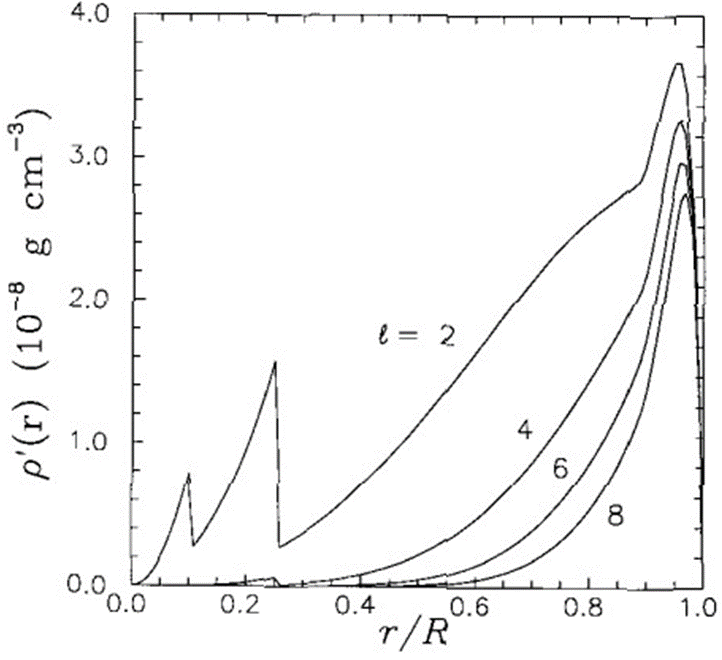
\includegraphics[width=0.5\textwidth]{marley_and_porco.png}
\caption{Density variation (perturbation) $\rho^{'}(r)$ versus scaled radial distance from the center to the surface of the planet \cite{Marley1993PlanetaryAM}.} \label{fig:my_label}
\end{figure}


Many gas giant models assume that amplitudes are smooth functions of frequencies, $l$ and $m$, as given in \cite{PMID:36042221}. This paper does an analysis of potential normal mode signals in Jupiter’s gravitational field, which could be comparable to the amplitudes of Saturnian normal-mode oscillations. In particular, for the figure extracted, the points marked $“f”$ on those plots are some of the same fundamental modes we are looking at in Saturn’s rings. Note the figure gives these signals in terms of zonal harmonic coefficients, which was gotten from potential amplitudes, through Juno spacecraft gravity measurements. Based on the results in \cite{PMID:36042221}, it is clearly evident that the normal-mode amplitudes for Jupiter varies increasingly, and smoothly, with decreasing angular degrees, $l$. Having a similar result for Saturn, and what such trends might look like, will pave the way for more understanding about its interior dynamics.
\begin{figure}[h] 
\centering
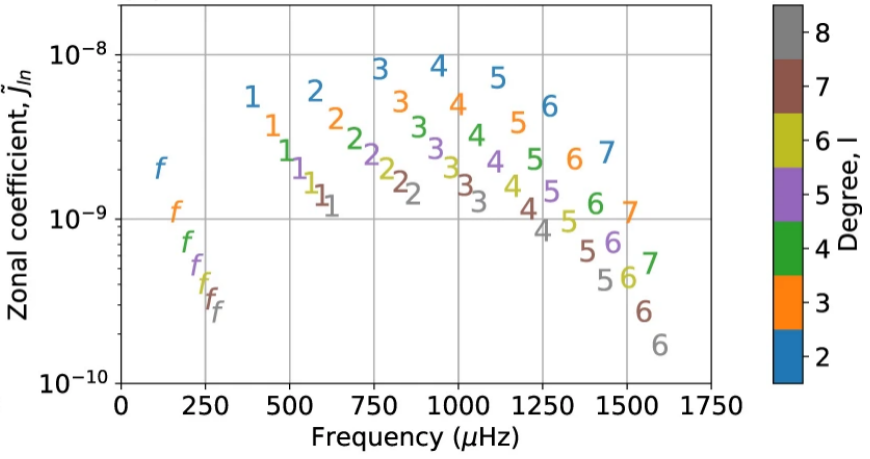
\includegraphics[width=0.6\textwidth]{durante.png}
\caption{The letters f and the numbers indicate, f-modes and the radial order of p-modes (up to n = 7) \cite{PMID:36042221}.} \label{fig:my_label}
\end{figure}

Finally, there are not yet measurements of individual planetary normal-mode amplitudes for Saturn. A catalogue of such measurements will assist with an accurate description of different excitation sources that could produce different signals at different values of oscillation frequencies, $l$ and $m$.

%from \cite{Marley1993PlanetaryAM},  similar research has been done at Jupiter, and the results show that, normal (fill in the blanks and attach diagrams/figures)...likewise, from \

Starting from the planet, and further out within the stretch of the C-ring, we aim to discuss the nature of Saturn's oscillatory phenomenon and how it initiates its effect across the particles located along the ring plane. We shall also lay the theoretical framework that explains the most profound phenomenon across the C-ring, the spiral density wave, as well as the corresponding normal-mode amplitudes responsible for the aforesaid phenomenon, which could serve as a link towards knowing what makes the planet ring (acoustically). However, before delving into these complexities, let us embark on an intriguing journey through seismological phenomena on a galactic scale, ultimately returning to Saturn and its remarkable rings.

%..............................................................................................
\section{Background: From Galaxy To Rings}

At the largest scales, galaxies exhibit oscillatory behavior in the form of density waves. Spiral galaxies, for example, often display prominent spiral arms that result from the propagation of density waves through their disk. These waves cause regions of higher density to compress, leading to star formation, while other regions experience lower density, resulting in relative voids. The dynamics of density waves in galaxies are described by equations such as the Toomre instability criterion given by\cite{2008gady.book.....B, 2002MNRAS.336..785S, 1964ApJ...139.1217T}:
\begin{equation}
Q = \frac{\kappa \cdot \sigma}{\pi \cdot G \cdot \Sigma},
\end{equation}
where \(Q\) is the Toomre parameter, \(\kappa\) is the epicyclic frequency, representing the frequency of radial oscillations in a rotating disk; \(\sigma\) is the velocity dispersion (random motion of particles) in the disk, \(G\) is the gravitational constant, \(\pi\) is the mathematical constant pi, \(\Sigma\) is the surface density of the disk.
This criterion helps determine whether a galactic disk is stable against axisymmetric gravitational instabilities and internal motions. If \(Q\) is greater than a critical value (typically around 1.5 to 2), the disk is considered stable. If \(Q\) falls below this critical value, the disk may become prone to the formation of spiral arms or other non-axisymmetric structures.

Moving to the scale of individual stars within galaxies, asteroseismology becomes a powerful tool for understanding their internal structure and evolution. Asteroseismology, the study of stellar oscillations, provides invaluable insights into the internal structure, composition, and evolution of stars. These oscillations, akin to seismic waves on Earth, are driven by the interplay of gravity, pressure, and nuclear reactions within stellar interiors. The frequencies and modes of oscillation carry crucial information about a star's properties, including its mass, radius, temperature, and chemical composition. One key aspect of asteroseismology is the distinction between different types of oscillations, such as radial, non-radial, and global modes, each revealing distinct features of a star's structure.

Radial oscillations involve expansion and contraction of a star's entire structure, similar to pulsations, about its equilibrium position. They are characterized by changes in radius without significant changes in shape. The periods of radial oscillations are determined by the star's density profile and can be described by the pulsation equation:
\begin{equation}
P_{e} = 2\pi \sqrt{\frac{R^3}{GM}}
\end{equation}
where $P_{e}$ is the period, \(R\) is the star's radius, \(G\) is the gravitational constant, and \(M\) is the star's mass.

Non-radial oscillations, on the other hand, involve changes in the star's shape without significant variations in its overall size. These oscillations manifest as surface waves or internal gravity waves, revealing information about the star's internal structure and rotation. Non-radial modes are characterized by spherical harmonic functions and can be described by equations such as the Laplace tidal equations. The radial oscillation could be seen as a special case of the nonradial oscillations, charaterized by the spherical harmonic index, $\ell = 0$.

Global oscillations encompass a wide range of frequencies and modes, reflecting the entire spectrum of oscillatory behavior within a star. By analyzing the frequencies and amplitudes of these oscillations, the star's internal conditions can be probed, such as the presence of convective zones, chemical gradients, and magnetic fields. These observations provide constraints for theoretical models of stellar structure and evolution.

In addition to the pulsation equation mentioned earlier, another important equation in asteroseismology is the Brunt-Väisälä frequency (\(N\)), which characterizes the stability of a stratified fluid medium such as a star's interior. This equation is particularly relevant for understanding the propagation of internal gravity waves and their influence on stellar oscillations\cite{unno1989nonradial}:
\begin{equation}
    N^{2} = g \left( \frac{1}{\Gamma_1} \frac{d\ln p_{0}}{dr} - \frac{d\ln\rho_{0}}{dr} \right),
\end{equation}
where \(N\) is the Brunt-Väisälä frequency, representing the natural frequency of oscillation of a fluid element in a stable environment, \(g\) is the local gravitational acceleration, which varies with radial distance within the star. \(\Gamma_1\) is the adiabatic exponent, which describes the relationship between pressure and density changes in an adiabatic process; mathematically it is given as $\Gamma_{1} = (d\ln p/d\ln \rho)_{ad}$. $p_{0}$ is the pressure within the star, and $\rho_{0}$ is the density. Both pressure and density vary with radial distance (\(r\)) within the star. \(d\ln P/dr\) and \(d\rho/dr\) represent the logarithmic derivatives of pressure and density with respect to the radial coordinate, respectively.

This equation highlights the role of buoyancy forces (\(N^2 > 0\)) in stabilizing or destabilizing a fluid element as it moves vertically within the star. Regions where \(N^2\) is positive are stable against vertical displacements, while regions with negative \(N^2\) are unstable, potentially leading to oscillatory motion.

Additionally, the equations governing the behavior of non-radial oscillations, such as the Laplace tidal equations, involve spherical harmonic functions and can be quite complex. These equations describe the propagation of waves within the star's interior, taking into account factors such as rotation, magnetic fields, and internal structure.

Generally, achieving the equilibrium configuration of stars requires three essential types of stability: dynamical stability, which includes vibrational stability, and thermal stability. Dynamical stability ensures the balanced interaction between the pressure gradient and gravitational forces within the star. For example, a slight contraction of a star increases the pressure gradient, which can counteract the gravitational force, thereby restoring the equilibrium state of the stellar system. Dynamical stability also encompasses considerations of angular momentum and the overall dynamics of the stellar system. Vibrational stability, a subset of dynamical stability, pertains to the oscillations of the star in response to perturbations. A dynamically stable system will undergo oscillations upon being perturbed by an arbitrary influence. These oscillations may not always be immediately visible, but they are indicative of the system's stability. If oscillations grow over time, the system is considered unstable. Thermal stability ensures that the star maintains a stable internal temperature distribution. This stability is crucial for maintaining the balance between the energy generated by nuclear fusion processes in the stellar core and the energy radiated away from the surface\cite{unno1989nonradial}.

\paragraph{Non-adiabatic Nonradial Oscillations:}

Nonradial oscillations, also known as non-spherical or non-radial pulsations, occur in stars when the equilibrium between inward gravitational forces and outward pressure forces is disturbed, causing the star to undergo periodic changes in shape and size. These oscillations are complex phenomena and are classified into various types, including p-modes (pressure modes), g-modes (gravity modes), and mixed modes, depending on the restoring force dominating the oscillation. 

Non-adiabatic nonradial oscillations in stars refer to pulsations where the assumption of adiabaticity, meaning that the heat exchange within the star is negligible during the pulsation cycle, does not hold. In these oscillations, energy exchange through radiation or convection significantly affects the behavior of the pulsations.These sorts of pulsations occur when the timescale of the pulsation is comparable to or shorter than the timescale of energy transfer processes such as radiation diffusion or convective mixing. As a result, the temperature and pressure within the star can change dynamically during the pulsation cycle.

When both non-adiabatic effects and nonradial oscillations are present, the behavior of the pulsations becomes even more intricate, as the energy exchange mechanisms interact with the spatial variations in the pulsation modes. This interaction can lead to phenomena such as mode coupling (explained below), where one type of oscillation affects the behavior of another, and mode switching, where the dominant pulsation mode changes over time. Understanding non-adiabatic nonradial oscillations is crucial for accurately modeling and interpreting the observed variability in stars, as they provide valuable insights into the internal structure, composition, and evolution of stellar objects. Here, we will focus on providing an overview of the wave equations and concepts involved in describing nonadiabatic nonradial oscillations, for the case of rotating stars.

To start with, we present the corresponding expressions describing the aforesaid oscillations, for the case of a rotating star. The first two expressions are those of the flux perturbation, $\textbf{F}^{'}$, given in terms of the radial gradient as\cite{unno1989nonradial}:
\begin{equation}
    F^{'}_{r} = - K\frac{\partial T^{'}}{\partial r} - K^{'}\frac{\partial T}{\partial r}
\end{equation}
and 
\begin{equation}
    \mathbf{F}^{'}_{\perp} = - K\nabla_{\perp}T^{'}.
\end{equation}

The thermodynamic relation between the perturbations of the pressure, temperature and entropy is given as\cite{hansen2004stellar, unno1989nonradial}:
\begin{equation}
    \frac{\delta T}{T} = \frac{\Gamma_{2}-1}{\Gamma_{2}}\frac{\delta p}{p} + \frac{\delta S}{c_{p}},
\end{equation}
where 
\begin{equation}
\frac{\Gamma_{2}-1}{\Gamma_{2}} \equiv \left( \frac{\partial \ln T}{\partial \ln p} \right)_{S} \quad \text{and} \quad c_{p} \equiv T \left( \frac{\partial S}{\partial T} \right)_{p}.
\end{equation}

Additionally, the linearized mass-conservation and energy equations can be given as \cite{aerts2010asteroseismology, hansen2004stellar, pedlosky2013geophysical, unno1989nonradial}:
\begin{equation}
    \left( \frac{\partial}{\partial t} + \mathbf{\Omega} \frac{\partial}{\partial \phi} \right)\rho' + \nabla\cdot(\rho_{0}\mathbf{v'}) = 0,
\end{equation}
and
\begin{equation}
    \rho_{0}T_{0}\left[\left( \frac{\partial}{\partial t} + \mathbf{\Omega} \frac{\partial}{\partial \phi} \right)\mathbf{S'} + (\mathbf{v}\cdot \nabla)\mathbf{S_{0}} \right] = (\rho\varepsilon_{N})' - \nabla \cdot \mathbf{F'_{R}}.
\end{equation}
The operator $\left( \frac{\partial}{\partial t} + \mathbf{\Omega} \frac{\partial}{\partial \phi} \right)$ is the temporal derivative specific to a local rotating frame having the angular velocity $\mathbf{\Omega}$.

To finalize the equations of motion, we can combine the time derivative of the velocity specific to a local rotating frame (first term) with the Coriolis force (second term), as well as the influence of differential rotation, as described in the equation\cite{aerts2010asteroseismology, hansen2004stellar, pedlosky2013geophysical, unno1989nonradial}:
\begin{equation}
     \left[\left( \frac{\partial}{\partial t} + \mathbf{\Omega} \frac{\partial}{\partial \phi} \right)\nu'_{i}\right]\mathbf{e_{i}} + 2\mathbf{\Omega\times v'} + \mathbf{(v'\cdot\nabla\Omega)}r\sin\theta \mathbf{e_{\phi}} = -\frac{1}{\rho_{0}}\nabla p' - \nabla \Phi' + \frac{\rho'}{\rho_{0}^{2}}\nabla p_{0},
\end{equation}
where the $\mathbf{v'}$ is the Eulerian velocity perturbation, and is related to the Lagrangian displacement $\mathbf{\xi}$, by the equation:
\begin{equation}
    \mathbf{v'} =  \left[\left( \frac{\partial}{\partial t} + \mathbf{\Omega} \frac{\partial}{\partial \phi} \right)\xi_{i}\right]\mathbf{e_{i}} - \mathbf{(\xi \cdot\nabla\Omega)}r\sin\theta \mathbf{e_{\phi}}
\end{equation}

The Poisson's Equation applicable for this case, is also given as\cite{Carroll_Ostlie_2017, unno1989nonradial}:
\begin{equation}
\nabla^2 \Phi = 4\pi G \rho.
\end{equation}
This equation relates the gravitational potential (\(\Phi\)) to the mass density (\(\rho\)), where \(\nabla^2\) is the Laplacian operator. Another equation of interest is the entropy perturbation written in terms of the Eulerian density and pressure perturbations\cite{1983psen.book.....C, unno1989nonradial}:
\begin{equation}
    \left( \frac{\partial}{\partial t} + \mathbf{\Omega} \frac{\partial}{\partial \phi} \right)\left( \frac{\rho'}{\rho_{0}} - \frac{p'}{\Gamma_{1}p_{0}} \right) + {\mathbf{v'}} \cdot \left( \nabla \ln \rho_{0} - \frac{1}{\Gamma_{1}} \nabla \ln p_{0} \right) = -\frac{\nu_{T}}{c_{p}}\left( \frac{\partial}{\partial t} + \mathbf{\Omega} \frac{\partial}{\partial \phi} \right) \delta S.
\end{equation}
%............................................................................................
\paragraph{Mode Classification:}

In the case of stars and planets, nonradial oscillations can be further subdivided into three main categories: p-modes, g-modes, and f-modes. \textbf{Pressure modes (p-modes)} are characterized by restoring forces related to pressure fluctuations. They dominate in the outer regions of the star where the pressure gradient is the main restorative force. \textbf{Gravity modes (g-modes)} are characterized by buoyancy as the dominant restoring force. They are prevalent in the deep interior of the star where gravity is the main restoring force. \textbf{Mixed modes} are hybrid modes that exhibit characteristics of both p-modes and g-modes. They often occur in intermediate regions of the star\cite{unno1989nonradial}. Examples of such modes are the f-modes, also known as the fundamental mode; they represent the fundamental oscillation mode observed in either p-modes or g-modes.

The principles of asteroseismology can also be extended to other celestial objects, such as planets like Saturn. While the scales and mechanisms differ, Saturn's oscillations, observed through atmospheric waves and internal dynamics, share similarities with stellar oscillations. For instance, the analysis of Saturn's oscillations provides insights into its atmospheric composition, internal structure, and gravitational interactions. By studying the frequencies and modes of oscillation in Saturn's atmosphere and interior, scientists can deepen their understanding of planetary dynamics and evolution. In summary, asteroseismology offers a powerful tool for investigating the internal properties of stars through the analysis of their oscillations. By extending these principles to other celestial bodies like Saturn, researchers can broaden their understanding of planetary dynamics and evolution, furthering our knowledge of the universe's diverse phenomena.

\subsection{The Saturnian Oscillations}
Saturnian oscillations, which are characterized by their fluid nature, are classified based on the types of displacements that occur during their propagation \cite{Marley1993PlanetaryAM}. 
%..............................................................................................................
%The Saturnian oscillations, being fluidic in nature, are classified in terms of radial and nonradial displacements produced during propagation \cite{Marley1993PlanetaryAM}. Typically for stars and planets, there are basic subclasses of nonradial oscillations responsible for nonradial displacements during propagation: the p-modes, the g-modes, and the f-modes. The p-modes are synonymous with resonant acoustic disturbances whose dominant restoring force is pressure. Likewise, the g-modes are synonymous with resonant internal gravitational disturbances, with their dominant restoring force as gravity. The f-modes, an acronym for fundamental mode, is the basic mode of either the aforesaid p-mode or the g-mode.
%..............................................................................................................

Considering the largest perturbations to external gravitational field \cite{article, Mankovich_2019, Marley1993PlanetaryAM}, a Saturnian oscillation mode creates a density perturbation inside the planet, which in turn creates a time-dependent Eulerian perturbation to its bulk property (the mass density corresponding
to the $lmn$ normal mode in the planet) is expressed in terms of surface spherical harmonics, $Y_{l}^{m}(\theta,\phi)$ as: 
\begin{equation}
    \rho_{lmn}^{'}(r,\theta,\phi,t) =   \rho_{lmn}^{'}(r)Y_{l}^{m}(\theta,\phi)e^{-i\sigma_{lmn}t},
\end{equation}
$\sigma_{lmn}$ is the mode oscillation frequency in the corotating frame with the planet. $r$ is the radius, $\theta$ is the colatitude, and $\phi$ is the azimuth angle respectively. The surface spherical harmonics, $Y_{l}^{m}(\theta,\phi)$, is given in terms of the associated Legendre polynomials as: 
\begin{equation}
     Y_{l}^{m}(\theta,\phi) = (-1)^{(m+|m|)/2} \sqrt{\frac{(2l+1)}{4\pi}\frac{(l-|m|)!}{(l+|m|)!}}P^{m}_{l} (\cos\theta)e^{im\phi}
\end{equation}
$\forall$  $l \in [0, \infty)$ and $m \in [-l,+l]$.

Alternatively, we can express other properties of the planetary oscillations using similar description, for example the pressure, P, or the gravitational potential, $\Phi$, in place of the density, $\rho_{lmn}^{'}(r,\theta,\phi,t)$.

In the field of seismology, we generally describe an oscillation-mode in terms of three integers, namely l, m, and n. Projecting these integers on a spherical surface, the angular degree, $l$, measures the number of circles bounding the regions of positive and negative perturbations. The oscillation's azimuthal order, $|m|$ $(m = -l, -l+1, ..., 0,..., l-1, l)$, accounts for the number of great circles passing through the polar axis that form longitudinal boundaries. The quantity, $l-|m|$, accounts for the number of latitudinal circles forming latitudinal boundaries, while $2|m|$ accounts for zero crossings in the longitudinal direction. 

Furthermore, we can visualize the planetary oscillations using few simple properties of the spherical harmonic functions. When the angular order $m$ is zero, the harmonics are called zonal and oscillate only in the latitudinal direction. When $l=|m|$ the harmononic are called sectoral and oscillate only in the longitudinal direction.  For other values of $m$ the harmonics are called tesseral and oscillate in both the longitudinal and latitudinal directions. The equivalent Cartesian wavelength for a spherical harmonic function of degree $l$ is approximately given as, $\lambda = 2\pi R/\sqrt{l(l+1)}$. R is the radius of the sphere, and this result is known as the Jeans relation \cite{https://doi.org/10.1029/2018GC007529}.


Interestingly, when $l-m$ is even, such modes are symmetric about the equator and tend to produce periodic radial gravitational perturbations in the equatorial plane, which are responsible for driving spiral density waves in the rings. But when $l-m$ is odd, such modes are anti-symmetric and are located about the equator. They produce periodic vertical perturbations in the equatorial plane, and are responsible for driving bending waves in the rings. The third integer, n, accounts for the number of radial nodes in the mode's density profile, between the center of the planet and its surface \cite{FRENCH2021114660}. When $n=0$, the mode is referred to as the fundamental-mode (f-mode). Also, when $m>0$, these modes rotate in the same direction as the planet (prograde), while $m<0$ modes rotate in opposite direction to the planet (retrograde). 

So far, the detected signals used in this work involve mostly modes with $l\geq 2$, and no $l=0$ modes, since they are not liable to generate noticeable external gravitational perturbations. A similar case holds for the dipolar f-modes ($l=1$), that are liable to generate fictitious oscillation in Saturn's center of mass \cite{FRENCH2021114660}.






From \cite{FRENCH2021114660, Marley1993PlanetaryAM}, suggestions have been made that the internal oscillations most likely to be responsible for driving density waves in the rings would be f-modes with $l=|m|$, the sectoral modes. These suggestions have been found to be true, following reported OLD-type density waves in the C-ring, with results consistent within the expectation values \cite{Hedman_2013, 10.1093/mnras/stu1503}. Another side to the previous results is the table showing the values for the mass estimates from the gravitational potentials, responsible for the spiral density wave amplitudes. The table clearly shows that none of these waves were excited by one or more of Saturn's moons, this implies that, most likely, the waves detected are as a result of planetary normal-mode oscillations (remember to add a diagram here).
\begin{figure}[h] 
\centering
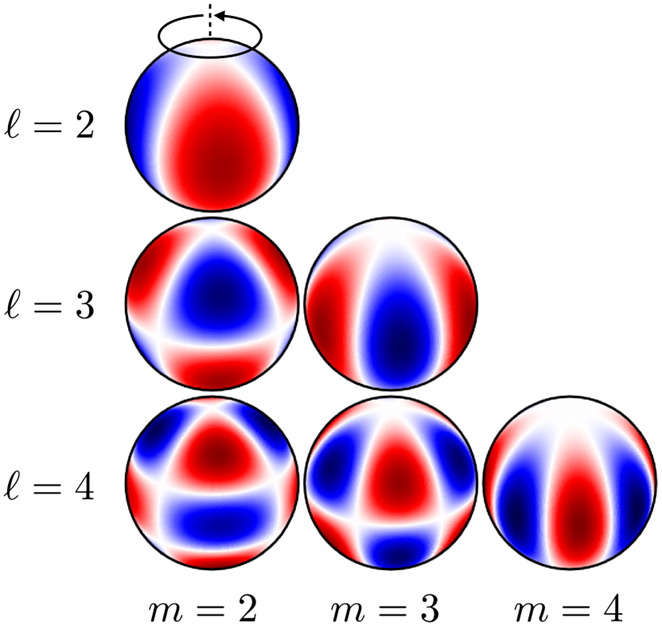
\includegraphics[width=0.5\textwidth]{mankovitch2.png}
\caption{A visual of some of the spherical harmonics relevant for Saturn ring seismology. $l$ denotes angular degree, while $m$ denotes azimuthal order \cite{Mankovich_2019}.  The color map corresponds to the magnitude of the density and gravity field perturbations, arising from oscillation. There is a downward trend of angular
degree ($l$) increase, and rightward increase in azimuthal order ($m$).} \label{fig:my_label}
\end{figure}

Understanding the aforesaid modes of oscillations help to clearly decipher the dynamics of this magnificent gas giant. Through the combination of observational data (Voyager and Cassini mostly) , theoretical models, and computer simulations, planetary scientists have been able to gain valuable insights into Saturn's internal structure, its atmospheric circulation, and the intricacies between its moons and the planet itself.

%So far, we are aware that the wave signals detected are not as a result of either one or more of Saturn's rings, based on measurements of mass estimates arising from the gravitational potentials of the wave signals detected, but as a result of the gravitational perturbations from Saturn (please see table below) .

%......Explain the process and attach equations where necessary...

%.............Add diagrams of different spherical harmonics for a sphere and use it to describe the acoustic oscillations of Saturn......



\subsection{Overview of Planetary Ring Seismology}

Planetary ring seismology is a field of study that uses the analysis of waves and vibrations within planetary rings to better understand their physical characteristics and formation history. By studying the way in which these waves propagate, researchers can gain insight into the density and composition of the particles within the rings, as well as the gravitational and tidal forces that influence their behavior.

On the other hand, planetary ring dynamics involves the study of the motion and behavior of particles within planetary rings. This could include the understanding of the gravitational, collisional, and electromagnetic forces that act on the particles, as well as the formation and evolution of the rings themselves.

By analyzing the distribution and behavior of the particles in a planetary ring, both areas of research can help provide researchers with more insight into the history and evolution of the planet and its moons. For example, the distribution of particles in Saturn's rings can provide information about the formation and evolution of Saturn's moon system. Also both fields could have implications for our understanding of planet formation and the evolution of planetary systems more broadly.


\subsection{The Ringmaster's Crown: Unveiling the Wonders of Saturn's Ring System}

Gazing skyward, few celestial objects capture our imagination quite like Saturn. Adorned with its iconic rings, this gas giant boasts the "most extensive and complex ring system" in our solar system. But what exactly are these rings made of, how did they form, and what secrets do they hold? Contrary to popular belief, Saturn's rings are not solid bands of ice. Instead, they consist of an estimated trillion individual ice particles, ranging in size from microscopic dust to massive boulders, stretching up to a kilometer across. Imagine a sprawling celestial city, not of buildings, but of countless icy moons, all orbiting the planet within a vast, flat disc. The main rings stretch from 7,000 Km to 280,000 Km away from Saturn's equator, while some fainter rings like the E-Ring extend much further, reaching all the way to the orbit of Saturn's moon, Titan \cite{enwiki:1201721965}.

These icy particles are primarily made of water ice, leftover from Saturn's formation billions of years ago, with traces of rocky materials and organic compounds called tholins\cite{NASA_Saturn}. These tholins contribute to the rings' intriguing color variations. The innermost rings appear dustier and somewhat reddish due to the presence of these complex molecules, while the outer rings gleam with a brighter, whiter hue dominated by water ice\cite{Britannica_Saturn}. Despite their icy composition, the rings are far from uniform. They are divided into thousands of individual rings and gaps, with seven prominent ones most easily visible. The A, B, and C rings are the densest and brightest, readily observable from Earth-based telescopes\cite{NASA_Saturn}. The Cassini Division, a dramatic gap between the B and A rings, hints at the complex forces shaping the system. Fainter rings like D, E, F, and G lie beyond, each with unique characteristics\cite{Britannica_Saturn}.

The exact formation of Saturn's rings remains a subject of ongoing research and debate. One leading theory suggests they originated from debris left over from the planet's formation\cite{enwiki:1201721965}. Another posits that they are the shattered remains of moons that strayed too close to Saturn's powerful gravity\cite{Britannica_Saturn}. Recent data from the Cassini mission, however, suggests a younger age for the rings, adding another layer of intrigue to the puzzle, leading to further investigation.

Saturn's rings are not static structures. The particles within them constantly interact, colliding, clumping, and even raining down onto the planet\cite{NASA_Saturn}. Spacecraft missions like Cassini have provided invaluable insights into the rings' secrets. Cassini spent 13 years orbiting Saturn, capturing stunning images and data that revolutionized our understanding of this magnificent system\cite{JPL_Cassini}. The future holds promise for further exploration, with missions like Dragonfly planned to land on one of Saturn's icy moons and potentially shed light on the rings' origins\cite{NASA_Dragonfly}.

Saturn's rings are more than just a beautiful adornment; they are a window into the planet's past, present, and even future. From their icy composition to their dynamic nature, these rings hold great potential for a better understanding not only of Saturn but also of the processes that shaped our solar system.


\subsection{Saturn’s C Ring}
Saturn's C ring is one of the most fascinating features of the sixth planet from the sun, spanning from about 74,658 km to 92,000 km from the planet's center, lying between the brighter B ring and the more diffuse D ring. The C Ring is made up of small particles ranging in size from micrometers to centimeters, and it is unique in that it has a peculiar wave-like pattern \cite{2009sfch.book..375C}\cite{Hedman_2018}\cite{Nicholson1990AnAR}. The waves across the C Ring were first observed by the Voyager spacecraft in the early 1980s. These waves are caused by gravitational interactions between the ring particles and Saturn's moons. As the moons pass by the ring, they create a gravitational disturbance that propagates through the ring in the form of a wave\cite{Hedman_2013}\cite{2014MNRAS.444.1369H}\cite{Hedman_2018}\cite{Marley1993PlanetaryAM}\cite{Nicholson1990AnAR}. These waves in the C Ring are incredibly precise, with wavelengths ranging from 30 to 180 kilometers. They are also very consistent, with the same patterns appearing year after year. The cause of this consistency is still not fully understood, but it is believed to be related to the structure of the ring particles themselves \cite{Hedman_2013}\cite{2014MNRAS.444.1369H}\cite{Hedman_2018}.

\begin{figure}[h] 
\centering
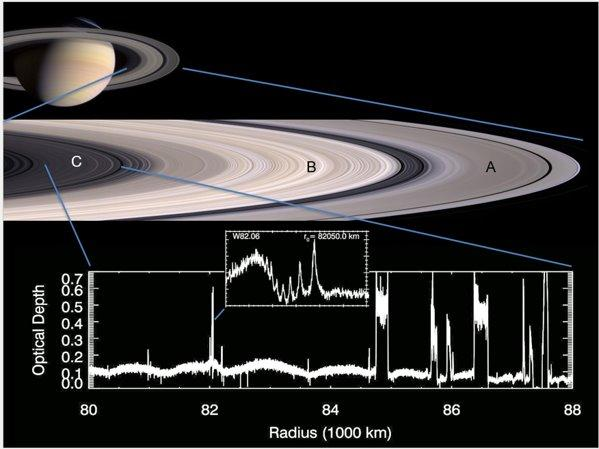
\includegraphics[width=0.7\textwidth]{Ring_Picture_Hedman_2018.jpg}
\caption{A picture of the A, B and C(Zoomed in) rings \cite{Hedman_2018}. An optical depth profile zoomed in on one of the waves (W82.06).} \label{fig:my_label}
\end{figure}



\subsection{Density Waves}
Spiral density and bending waves are well-researched and understood phenomena in the rings of Saturn, and they have provided valuable information about the surface mass density and viscosity of the main ring regions \cite{2009sfch.book..375C}\cite{Hedman_2013}\cite{2020AGUA....100142M}. The majority of these waves are caused by resonances with external satellites, especially in the A and B rings. However, another set of waves has been discovered in recent times, primarily in the C ring, which are not caused by satellites but by irregularities in Saturn's own gravitational field \cite{Hedman_2013}\cite{2014MNRAS.444.1369H}\cite{Hedman_2018}.Our focus is on studying the waves that are generated in Saturn's rings by the planetary normal modes. Specifically, we are exploring the inner C ring which has not been extensively researched before \cite{FRENCH2019599}\cite{Hedman_2013}. The waves in this area have very short wavelengths, which has posed a challenge for previous studies as they relied on precise calculations of wave phases to identify them \cite{FRENCH2019599}\cite{Hedman_2013}\cite{Hedman_2018}\cite{Tiscareno_2007}.In the next section, we aim to outline the basics of Fourier analysis and device an efficient algorithm for Fourier transformations, to use in processing Cassini's VIMS (Visual and Infrared Mapping Spectrograph) data, since other tested algorithms have resulted to an inefficient result. Thereafter, we will apply the new algorithm to our data and present the results achieved using this technique.




%\begin{figure}[h] 
%\centering
%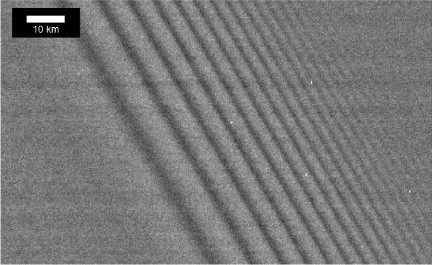
\includegraphics[width=0.7\textwidth]{Main_Wave_Web capture_3-4-2023_183537_reader.elsevier.com.jpeg}
%\caption{A portion of Cassini image N1467345975, showing the nearly-arche-typal Prometheus 9:8 [spiral] density wave \cite{Tiscareno_2007}.} \label{fig:my_label}
%\end{figure}
%................................................................................................................

\subsubsection{The Theory of Spiral Density Waves: Linear Density Wave Model}
In this section, we outline the concept of spiral density waves, how it is formed across Saturn's C ring and the mathematical representation of such phenomenon.
Basically, when normal-mode oscillations take place within gaseous planets, like Saturn, they do so in terms of vibrations, and these vibrations in turn give rise to variations in density within the planet, causing disturbances to be generated within the planet, and these disturbances in turn propagate towards the exterior of Saturn. Saturn's gravitational field simply couples these disturbances to the plane of the rings, and these disturbances travel across the stretch of the ring in form of density waves, spiral density and spiral bending waves. Our main focus is on the spiral density waves since their main cause are as a result of normal mode excitation within Saturn.


For a better understanding of this work on the spiral density wave analysis, we need to outline the theory behind the algorithms used in the subsequent sections.
Here, we are utilizing the density wave model to produce anticipated wave profiles \cite{Nicholson1990AnAR}. The specific model we are using is the linear, damped model which was originally derived and elaborately introduced by Shu in 1984 \cite{article}. To provide the essential details for our project, we will give a concise explanation of the model equations as well as the model parameters. This will help us to understand the workings of the model better and enable us to use it more effectively in our project. The linear, damped model is a well-established method that has been utilized in many scientific studies to describe a variety of astronomical phenomena.

%   EDITED SECTION NOVEMBER 2023. 
%   FULL DERIVATION FOR LINEAR DENSITY WAVEMODEL

Usually, when these waves are propagated across the ring, they are displayed as fluctuations in the density of the ring's surface, which affects its optical properties. This fluctuation has an m-fold symmetry and rotates with respect to the fixed reference frame at a rate of $\Omega_{p}$. The altered surface density distribution, normalized to the background density in areas outside the waves' region, $\sigma_{0}$, is represented by the expression \cite{Nicholson1990AnAR}:

\vspace{2pt}

\begin{equation}
\Delta \sigma(r,\lambda,t) = 1 + \Re\{-iA_{L}[\pi^{-1/2}-2i\xi H(\xi)]e^{i\phi}\}e^{-(\xi /\xi_{D})^{3}},
\end{equation}
The wave phase, $\phi$, and dimensionless distance from the resonance location, $\xi$, are clearly defined in the equations below, alongside $\xi_{D}$, which denotes the characteristic damping length of the wave. 

\vspace{2pt}
Simplifying the previous equation using Euler's identify, we have the variant below:
\begin{equation}
\Delta \sigma(r,\lambda,t) = 1 + \Re\{A_{L}e^{i(\phi-\pi/2)}[\pi^{-1/2}+2\xi e^{-i\pi/2}H(\xi)]\}e^{-(\xi/\xi_{D})^{3}}
\end{equation}

\vspace{2pt}

The function $H(\xi) = \pi^{-1/2}e^{-i\xi^{2}}\int_{-\infty}^{\xi}e^{i\eta^{2}}d\eta$. $H(\xi)$ includes the Standard Fresnel integral. Let $H(\xi) = \pi^{-1/2}e^{-i\xi^{2}}\gamma(\xi)$, so that the Standard Fresnel integral, $\gamma(\xi)$, is excluded from the function, $H(\xi)$. Thus we have the expression below:
\begin{equation}
    \gamma(\xi) = \int_{-\infty}^{\xi}e^{i\eta^{2}}d\eta
\end{equation}


Far into the region of wave propagation, $\xi$ is considered large and positive  \cite{Nicholson1990AnAR} \cite{1984prin.conf..513S}. Also considering the notion that the complex-Gaussian expression is exponentially convergent, we can simply separate the aforesaid integral for easy analysis resulting to the expression,
\begin{equation}
    \gamma(\xi) = \int_{-\infty}^{+ \infty}e^{i\eta^{2}}d\eta - \int_{\xi}^{\infty}e^{i\eta^{2}}d\eta = \gamma_{1} + \gamma_{2}
\end{equation}

\textbf{First Part of Integral:}
Here in this section, we are going to resolve the first part of the expanded integral for $\gamma(\xi)$, using contour integration. Let $\gamma_{1} = \int_{-\infty}^{+ \infty}e^{i\eta^{2}}d\eta$ and $\gamma_{2} = - \int_{\xi}^{\infty}e^{i\eta^{2}}d\eta$.

Considering $\gamma_{1}$, and since it is similar to the real Gaussian function, we devise a technique along the lines of Contour integration to bring it closer to the real Gaussian expression for easy analysis. Let,
\begin{equation}
    \gamma_{1} = \int_{-\infty}^{+ \infty}e^{i\eta^{2}}d\eta = 2\int_{0}^{+ \infty}e^{-(-i\eta^{2})}d\eta.
\end{equation}
Using polar coordinate expression for the arguments of $\gamma_{1}$, we have this as:
\begin{equation}
    \gamma_{1} = 2\int_{0}^{+ \infty}e^{-(e^{-i\pi/2} \eta^{2})}d\eta.
\end{equation}
We go on to factorize the previous equation and this results to, 
\begin{equation}
    \gamma_{1} = 2\int_{0}^{+ \infty}e^{-(e^{-i\pi/4} \eta)^{2}}d\eta.
\end{equation}
By substituting a variable for the exponential argument, we let $\rho = e^{-i\pi/4} \eta$ \cite{video}. Reshuffling the limits of our integral, we have: 
\begin{equation}
    \gamma_{1} = 2 e^{i\pi/4} \lim_{{R \to \infty}} \int_{0}^{Re^{-i\pi/4}} e^{-(\rho)^{2}} \, d\rho
\end{equation}

Let $\gamma_{1}^{'}$ represent the coefficient of 2 and the Euler argument in the main expression for $\gamma_{1}$, we have this as: $\gamma_{1}^{'} = \lim_{{R \to \infty}} \int_{0}^{Re^{-i\pi/4}} e^{-(\rho)^{2}} \, d\rho$, hence $\gamma_{1} = 2 e^{i\pi/4} \gamma_{1}^{'}$.

%............................................
\begin{figure}[h] 
\centering
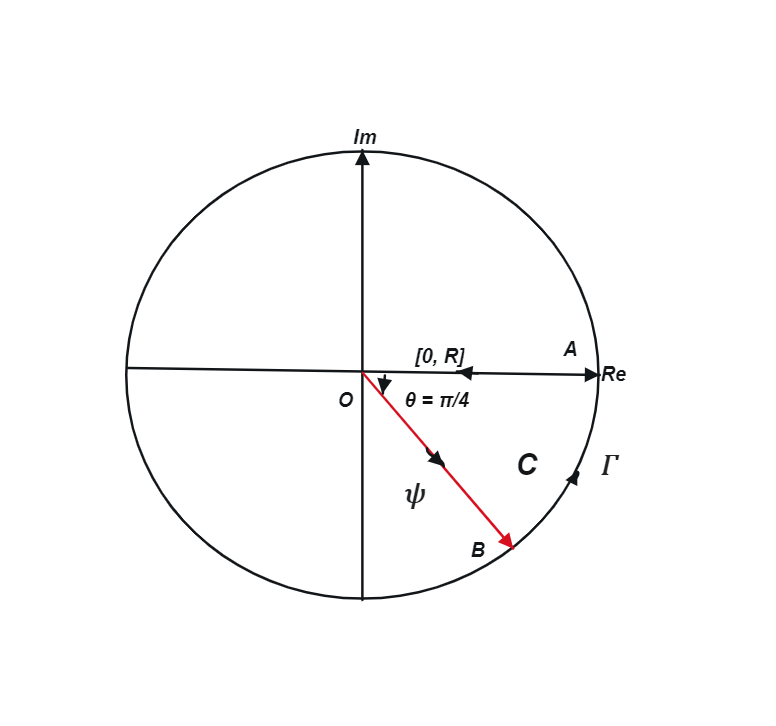
\includegraphics[width=0.6\textwidth]{COUNTOUR_INTEGRATION_DIAGRAM.png}
\caption{ Description of a pizza-shaped contour, consisting of the real (horizontal) and imaginary (vertical) axis.} \label{fig:my_label}
\end{figure}
%............................................

Considering the closed contour, as given in the diagram, for a pizza-shaped type of contour slice at an angle of $\pi/4$ radian (this angle also buttresses the asymptotic nature of $\xi$ \cite{Tiscareno_2007}), we can parametrize the previous expression and go on to evaluate the exact value of the Fresnel integral. This simply allows us to decomposed our contour integration according to the three sections present in our defined contour using complex analysis notations,
\begin{equation}
    \oint_{C} e^{-(z)^{2}} \, dz = \int_{\Psi} e^{-(z)^{2}} \, dz + \int_{\Gamma} e^{-(z)^{2}} \, dz + \int_{R}^{0} e^{-(z)^{2}} \, dz.
\end{equation}


Using Cauchy-Riemann's theorem, $\oint_{C} e^{-(z)^{2}} \, dz = 0$ (on the left hand side of the equation), since it is holomorphic inside and on $C$. Next, we consider the three sections of the given contour.

Given the conditions, $C = \left\{ z = x : 0 \leq x \leq R \right\} \cup \left\{ z : z = Re^{i\theta}, -\frac{\pi}{4} \leq \theta \leq 0 \right\} \cup \left\{ z : z = r,  0 \leq r \leq Re^{-i\frac{\pi}{4}}\right\}$, we can start with the line segment OB, $\Psi$. Here, 
\begin{equation}
    \int_{\Psi} e^{-(z)^{2}} \, dz = \int_{0}^{Re^{-i\frac{\pi}{4}}} e^{-(r)^{2}} \, dr.
\end{equation}
As $R \rightarrow \infty$, the integral along $\Psi$ assumes the format of a typical Gaussian integral, hence $\int_{0}^{\infty} e^{-(r)^{2}}\, dr = \frac{\sqrt{\pi}}{2}$.

Considering the arc BA, corresponding to the section $\Gamma$ of our contour integration,
\begin{equation}
    \int_{\Gamma} e^{-(z)^{2}} \, dz = \int_{-\frac{\pi}{4}}^{0} e^{-(z)^{2}} \, dz, \hspace{3pt} dz = iRe^{i\theta} d \theta. 
\end{equation}
By substitution we have the form for $\Gamma$ as,
\begin{equation}
    \int_{\Gamma} e^{-(z)^{2}} \, dz = \int_{-\frac{\pi}{4}}^{0} e^{-R^{2}e^{2i\theta}} iRe^{i\theta} d\theta. 
\end{equation}
Considering the absolute value of the given integral along the arc, $\Gamma$, this can be written as:
\begin{equation}
   \left| \int_{\Gamma} \right| \leq \int_{-\frac{\pi}{4}}^{0} \left|e^{-R^{2}e^{2i\theta}} iRe^{i\theta}\right| d\theta = R\int_{-\frac{\pi}{4}}^{0} \left|e^{-R^{2}e^{2i\theta}}\right| d\theta = R\int_{-\frac{\pi}{4}}^{0} \left|e^{-R^{2}[{\cos{(2\theta)} + i\sin{(2\theta)}}]}\right| d\theta.
\end{equation}
Using Euler's indentity, we reduce the expression to its real part only,
\begin{equation}
   \left| \int_{\Gamma} \right| \leq R\int_{-\frac{\pi}{4}}^{0}e^{-R^{2}\cos(2\theta)}d\theta.
\end{equation}
Intuitively, an integral like the one above with such property, vanishes as R becomes large. We are going to validate this claim analytically. A plot of $\cos(2\theta)$ $\forall \theta \in [-\frac{\pi}{4}, 0]$ simply shows that it has its minimum point at $-\frac{\pi}{4}$ and maximum point at $0$. We actually need a function within the same bound that best maximizes the $\cos(2\theta)$ within the exponential argument, to help validate our claim. An optimized function for this operation is $f(\theta) = \frac{4\theta}{\pi}+1$. This implies that, $\cos(2\theta) \geq f(\theta), \forall \theta \in [-\frac{\pi}{4}, 0]$.
Therefore, $e^{-R^{2}\cos(2\theta)} \leq e^{-R^{2}(\frac{4\theta}{\pi}+1)}$. Applying this to the previous case, 
\begin{equation}
   \left| \int_{\Gamma} \right| \leq R\int_{-\frac{\pi}{4}}^{0}e^{-R^{2}(\frac{4\theta}{\pi}+1)}d\theta = \frac{\pi}{4R}(1 - e^{-R^{2}})
\end{equation}
So we establish that, 
\begin{equation}
\lim_{{R \to \infty}} \left| \int_{\Gamma} \right| = \lim_{{R \to \infty}} \frac{\pi}{4R}(1 - e^{-R^{2}}) \leq 0.
\end{equation}

Next, we consider line segment OA, the real part of the contour. Redirecting the integral expression for that section, we have:
\begin{equation}
 \lim_{{R \to \infty}} \int_{R}^{0} e^{-(z)^{2}} \, dz = \lim_{{R \to \infty}} - \int_{0}^{R} e^{-(x)^{2}} \, dx = - \int_{0}^{\infty} e^{-(x)^{2}} \, dx = -\frac{\sqrt{\pi}}{2}.
\end{equation}

Recall, $\oint_{C} e^{-(z)^{2}} \, dz = \int_{\Psi} e^{-(z)^{2}} \, dz + \int_{\Gamma} e^{-(z)^{2}} \, dz + \int_{R}^{0} e^{-(z)^{2}} \, dz.$ Using the answers to each integral, $0 = \frac{\sqrt{\pi}}{2} + 0 - \frac{\sqrt{\pi}}{2}$, which is \textbf{true}. This shows that, $\gamma_{1}^{'} = \frac{\sqrt{\pi}}{2}$ and $\gamma_{1} = \sqrt{\pi}e^{i\pi/4}$.

\vspace{3pt}

\textbf{Second Part of Integral:}
For the case of $\gamma_{1}$, we could decompose it into a standard Fresnel integral and an integral that behaves like a Fresnel function as its argument approaches infinity. Here,
\begin{equation}
\gamma_{2} = - \int_{\xi}^{\infty}e^{i\eta^{2}}d\eta = -\int_{0}^{\infty}e^{i\eta^{2}}d\eta + \int_{0}^{\xi}e^{i\eta^{2}}d\eta = -\frac{\sqrt{\pi}}{2}e^{i\frac{\pi}{4}} + \int_{0}^{\xi}e^{i\eta^{2}}d\eta.
\end{equation}
Using the de Moivre's theorem, $\int_{0}^{\xi}e^{i\eta^{2}}d\eta = \int_{0}^{\xi}[cos(\eta^{2}) + isin(\eta^{2})]d\eta$. Let $C(\xi) = \int_{0}^{\xi}\cos(\eta^{2})d\eta$ and $S(\xi) =  \int_{0}^{\xi}\sin(\eta^{2})d\eta$ assume the real and imaginary parts of the asymptotic Fresnel expressions, respectively, so that $\int_{0}^{\xi}e^{i\eta^{2}}d\eta = C(\xi) + iS(\xi)$.

\vspace{5pt}

We can express the asymptotic behaviour of the aforesaid Fresnel integrals using the given forms as \cite{abramowitz1968handbook}\cite{enwiki:1181389148}\cite{wolfram-alpha-notebook}: 
\begin{equation}
    C(\xi) = \sqrt{\frac{\pi}{8}}\,\text{sgn}(\xi) + \left[1 + \mathcal{O}\left(\xi^{-4}\right)\right]\left(\sin(\xi^2)\left(\frac{1}{2\xi}\right) + \cos(\xi^2)\left(-\frac{1}{4}\,\mathcal{O}\left(\xi^{-3}\right)\right)\right)
\end{equation}
and
\begin{equation}
   S(\xi) = \sqrt{\frac{\pi}{8}}\,\text{sgn}(\xi) - \left[1 + \mathcal{O}\left(\xi^{-4}\right)\right]\left(\cos(\xi^2)\left(\frac{1}{2\xi}\right) + \sin(\xi^2)\left(\frac{1}{4}\,\mathcal{O}\left(\xi^{-3}\right)\right)\right).
\end{equation}


In the case of our model, we assume a moderate propagation of the density waves, which implies that as $\xi \rightarrow \infty$, $\mathcal{O}(\xi^{-n}) \rightarrow 0$ $\forall$ $n>1$. The moderated expression for the Fresnel integrals becomes, 
\begin{equation}
\int_{0}^{\xi}e^{i\eta^{2}}d\eta = \sqrt{\frac{\pi}{8}}\,\text{sgn}(\xi) + \frac{\sin(\xi^2)}{2\xi} + i\left(\sqrt{\frac{\pi}{8}}\,\text{sgn}(\xi) - \frac{\cos(\xi^2)}{2\xi}\right) = \frac{1}{2}\left[\sqrt{\pi}e^{i\frac{\pi}{4}}\,\text{sgn}(\xi) - \frac{i}{\xi}e^{i\xi^{2}}\right].
\end{equation}
Therefore, 
\begin{equation}
\gamma_{2} = \frac{\sqrt{\pi}}{2}e^{i\frac{\pi}{4}}\left[\,\text{sgn}(\xi) - 1\right] + \frac{e^{i(\xi^{2} - \pi/2)}}{2\xi},
\end{equation}
so that $\gamma(\xi) = \frac{\sqrt{\pi}}{2}e^{i\frac{\pi}{4}}\left[\,\text{sgn}(\xi) + 1\right] + \frac{e^{i(\xi^{2} - \pi/2)}}{2\xi}$.

Now, we re-express  $H(\xi)$ as follows, 
\begin{equation}
    H(\xi) = \frac{e^{i(\frac{\pi}{4} - \xi^{2})}}{2}\left[\,\text{sgn}(\xi) + 1\right] + \frac{e^{i(-\pi/2)}}{2\xi \sqrt{\pi}}
\end{equation}

Considering the linear density wave equation, $\Delta \sigma(r,\lambda,t)$, this becomes:
\begin{equation}
 \Delta \sigma(r,\lambda,t) = 1 + \Re\{A_{L}e^{i(\phi-\pi/2)}[\pi^{-1/2} + \xi e^{-i{(\pi/4 + \xi^{2})}}\left[\,\text{sgn}(\xi) + 1\right] + \pi^{-1/2}e^{-i\pi}]\} e^{-(\xi/\xi_{D})^{3}}
\end{equation}

\begin{equation}
\Delta \sigma(r,\lambda,t) = 1 + \Re\{A_{L}e^{i(\phi-\pi/2)}[\xi e^{-i{(\pi/4 + \xi^{2})}}\left[\,\text{sgn}(\xi) + 1\right]]\} e^{-(\xi/\xi_{D})^{3}}
\end{equation}


\begin{equation}
\Delta \sigma(r,\lambda,t) = 1 + \Re\{A_{L}[\xi e^{i{(\phi - 3\pi/4 - \xi^{2})}}\left[\,\text{sgn}(\xi) + 1\right]]\} e^{-(\xi/\xi_{D})^{3}}
\end{equation}

Using the de Moivre's theorem as well as the real part of the linear density wave equation, this expression becomes as:
\begin{equation}
\Delta \sigma(r,\lambda,t) = 1 + {\{A_{L}\xi\left[\,\text{sgn}(\xi) + 1\right]\cos{(\phi - 3\pi/4 - \xi^{2})}}\}e^{-(\xi/\xi_{D})^{3}}
\end{equation}


Removing the "unit" vertical translation, and considering both directions of wave propagations, this results to the given expression: 
\begin{equation}
   \Delta \sigma(r,\lambda,t) = A_{L}\xi\\e^{-\left(\frac{\xi_{*}}{\xi_{D}}\right)^3}\cos\left(\phi-\frac{3\pi}{4}-\xi^2\right)\zeta(\xi_{*})
\end{equation}

Where $\zeta(\xi_{*})$ encompases a generalized signum function, $\zeta(\xi_{*}) = [1 + \mathrm{sgn}(m)\mathrm{sgn}(\xi)]$  and $ \mathrm{sgn}(\xi) = \left\{ \begin{array}{rcl}
1 & \forall
& \xi>0 \\ 0 & \forall & \xi=0 \\ -1 & \forall & \xi<0 \\
\end{array}\right\}$.

\vspace{3pt}

Here, $\sigma(r,\lambda,t)$ is the perturbed surface density distribution of the ring section, $r$ is the distance (in kilometers) away from the center of the planet, $\lambda$ and $t$ are the longitude and time of observation, respectively. $A_{L}$ is the dimensionless amplitude factor, it is dependent on the mass of the perturbing moon, inducing the wave \cite{Tiscareno_2007}. $\phi = m(\lambda_{s}(0)+\Omega_{s}t-\lambda$) is the wave phase; $\lambda_{s}(0)$ is the mean longitude of the satellite at $t=0$ and $\Omega_{s}$ is the orbital mean motion of the satellite. $\xi_{D}$ is the dimensionless damping parameter, which depicts the location at which the wave's amplitude ceases to grow and begins to decay. It is also sensitive to the viscosity of the ring \cite{Tiscareno_2007}.
From \cite{Nicholson1990AnAR} \cite{1984prin.conf..513S}, $\xi$ is a dimensionless quantity that specifies the distance from the resonant radius, $r_{L}$, and it is given as:
\begin{equation}
\xi = \left[\frac{3|m-1|\Omega_{L}^{2}r_{L}}{4\pi G \sigma_{0}}\right]^{\frac{1}{2}}\left(\frac{r-r_{L}}{r_{L}}\right), 
\end{equation}
and $\xi_{*} = \xi \mathrm{sgn}(r - r_{L})$.

\vspace{3pt}

The resonant radius, $r_{L}$, fixes the wave against translation in the radial direction \cite{Tiscareno_2007}. Similarly, the background surface density, $\sigma_{0}$, controls the rate at which the wavenumber increases with respect to the wave's distance from its resonant location \cite{Tiscareno_2007}. $G$ is the Newtonian gravitational constant equivalent, in SI units, to $6.674 \times 10^{-11} \, \mathrm{m^3 \, kg^{-1} \, s^{-2}}$.

\textbf{Note:} $\zeta(\xi)$ is the general parameter used to account for spiral density waves with both positive and negative azimuthal orders, and such cases determine whether the sign of $\xi$ will either be positive or negative. We explain this in the wave-fitting routine.

\begin{figure}[h] 
\centering 
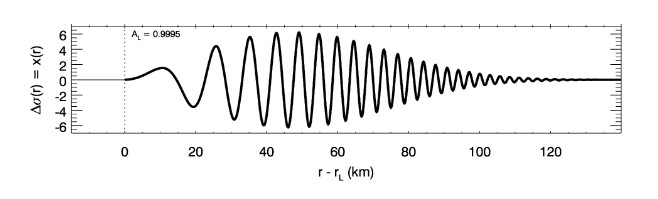
\includegraphics[width=1.0\textwidth]{Linear_Density_WM.jpg}
\caption{Synthetic density-wave radial profile generated by Equation (1) for a case of $m>0$ (prograde) \cite{Tiscareno_2007}.} \label{fig:my_label}
\end{figure}
%................................................................

%Usually, when these waves are propagated across the ring, they are displayed as fluctuations in the density of the ring's surface, which affects its optical properties. This fluctuation has an m-fold symmetry and rotates with respect to the fixed reference frame at a rate of $\Omega_{p}$. The altered surface density distribution, normalized to the background density in areas outside the waves' region, $\sigma_{0}$, is represented by the expression \cite{Nicholson1990AnAR}:

%\vspace{2}

%\begin{equation}
%\Delta \sigma(r,\lambda,t) = 1 + \Re\{A_{L}e^{i(\phi-\pi/2)}[\pi^{-1/2}+2\xi e^{-i\pi/2}H(\xi)]\}e^{-(\xi_{*} /\xi_{D})^{3}}
%\end{equation}

%\vspace{2}

%The function $H(\xi) = \pi^{-1/2}e^{-i\xi^{2}}\int_{-\infty}^{\xi}e^{i\eta^{2}}d\eta$. $H(\xi)$ includes the Standard Fresnel integral. Let $H(\xi) = \pi^{-\pi/2}e^{-i\xi^{2}}\gamma(\xi)$, so that $\gamma(\xi) = \int_{-\infty}^{\xi}e^{i\eta^{2}}d\eta$. Far into the region of wave propagation, $\xi$ is considered large and positive \cite{article}, resulting to the expression,
%\begin{equation}
 %   \gamma(\xi) = \int_{-\infty}^{+ \infty}e^{i\eta^{2}}d\eta - \int_{-\xi}^{\infty}e^{i\eta^{2}}d\eta = \frac{\sqrt{\pi}}{2}e^{i\pi/4} + \int_{0}^{\xi}e^{i\eta^{2}}d\eta.
%\end{equation}
%The first term was estimated using Cauchy-Riemann's integral formula alongside Jordan's Lemma, specifically for a pizza-shaped type of contour slice at an angle of $\pi/4$ radian (this angle also buttresses the asymptotic nature of $\xi$ \cite{Tiscareno_2007}). 

%\vspace{5}

%From \cite{abramowitz1968handbook}, $\int_{0}^{\xi}e^{i\eta^{2}}d\eta = \int_{0}^{\xi}\cos(\eta^{2})d\eta + i \int_{0}^{\xi}\sin(\eta^{2})d\eta = C(\xi) + i  S(\xi)$. $C(\xi)$ and $S(\xi)$ are the Fresnel integrals. As $\xi \rightarrow \infty$, $\mathcal{O}(\xi^{-n}) \rightarrow 0$ $\forall$ $n>1$. Thus: 
%$C(\xi) = \sqrt{\frac{\pi}{8}}sgn(\xi) + \frac{\sin(\xi^{2})}{2\xi}$ and $S(\xi) = \sqrt{\frac{\pi}{8}}sgn(\xi) - \frac{\cos(\xi^{2})}{2\xi}$. By substituting into the Fresnel integral and simplifying for a general case of positive azimuthal orders of the spiral density waves: 
%\begin{equation}
%\gamma(\xi) \approx \frac{\sqrt{\pi}}{2}[1 + sgn(\xi)]e^{i \pi/4} + \frac{e^{i(\xi^{2} - \pi/2)}}{2\xi}
%\end{equation}

%Finally, we put $H(\xi)$ into equation (1), and take the real part of the expression (neglecting the vertical translation). This results to the given expression: 
%\begin{equation}
 %   \Delta \sigma(r,\lambda,t) = A_{L}\xi\\e^{-\left(\frac{\xi_{*}}{\xi_{D}}\right)^3}\cos\left[\phi-\frac{3\pi}{4}-\xi^2\right]\zeta(\xi)
%\end{equation}

%Where $\zeta(\xi)$ encompases a generalized signum function, $\zeta(\xi) = [1 + \mathrm{sgn}(\xi)]$  and $ \mathrm{sgn}(\xi) = \left\{ \begin{array}{rcl}
%1 & \forall
%& \xi>0 \\ 0 & \forall & \xi=0 \\ -1 & \forall & \xi<0 \\
%\end{array}\right\}$.

%\vspace{3}

%Here, $\sigma(r,\lambda,t)$ is the perturbed surface density distribution of the ring section, $r$ is the distance (in kilometers) away from the center of the planet, $\lambda$ and $t$ are the longitude and time of observation, respectively. $A_{L}$ is the dimensionless amplitude factor, it is dependent on the mass of the perturbing moon, inducing the wave \cite{Tiscareno_2007}. $\phi = m(\lambda_{s}(0)+\Omega_{s}t-\lambda$) is the wave phase; $\lambda_{s}(0)$ is the mean longitude of the satellite at $t=0$ and $\Omega_{s}$ is the orbital mean motion of the satellite. $\xi_{D}$ is the dimensionless damping parameter, which depicts the location at which the wave's amplitude ceases to grow and begins to decay. It is also sensitive to the viscosity of the ring \cite{Tiscareno_2007}.
%From \cite{Nicholson1990AnAR} \cite{1984prin.conf..513S}, $\xi$ is a dimensionless quantity that specifies the distance from the resonant radius, $r_{L}$, and it is given as:
%\begin{equation}
%\xi = \left[\frac{3|m-1|\Omega_{L}^{2}r_{L}}{4\pi G \sigma_{0}}\right]^{\frac{1}{2}}\left(\frac{r-r_{L}}{r_{L}}\right), 
%\end{equation}
%and $\xi_{*} = \xi \mathrm{sgn}(r - r_{L})$.

%\vspace{3}

%The resonant radius, $r_{L}$, fixes the wave against translation in the radial direction \cite{Tiscareno_2007}. Similarly, the background surface density, $\sigma_{0}$, controls the rate at which the wavenumber increases with respect to the wave's distance from its resonant location \cite{Tiscareno_2007}. G is the Newtonian gravitational constant equivalent, in SI units, to $6.674 \times 10^{-11} m^{3}⋅kg^{-1}⋅s^{-2}$.
%\textbf{Note:} $\zeta(\xi)$ is the general parameter used to account for spiral density waves with both positive and negative azimuthal orders, and such cases determine whether the sign of $\xi$ will either be positive or negative. We explain this in the wave-fitting routine.

%\begin{figure}[h] 
%\centering 
%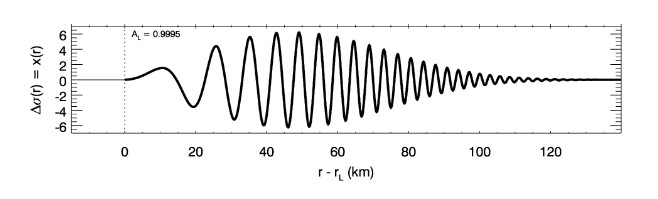
\includegraphics[width=1.0\textwidth]{Linear_Density_WM.jpg}
%\caption{Synthetic density-wave radial profile generated by Equation (1) for a case of $m>0$ (prograde) \cite{Tiscareno_2007}.} \label{fig:my_label}
%\end{figure}

%.................................................................
%.................................................................

\section{Methodology}
Having established the fundamental theoretical foundation for planetary oscillations and the associated effects across Saturn's (C)-ring(s), spiral density waves, our subsequent aim is to reinforce the mathematical tools employed in computing the necessary amplitudes of normal modes for Saturnian oscillations. The components of this toolbox are crucial in facilitating a precise and rigorous examination of the complex dynamics exhibited by spiral density waves, encompassing their periodic structures and frequencies.

\subsection{Wavelet Analysis}
 The method of Fourier transform provides us with valuable insights into the underlying physical properties of waves, which can be essential for understanding their behavior and predicting their future evolution. Ultimately, our application and interpretation of Fourier transform algorithms will help to shed light on the complex nature of spiral density waves and how they are excited from Saturn's interior.
 
Wavelet analysis is a method of time-frequency analysis that is scale independent and can provide more detailed information about the dominant frequencies present in a signal than traditional Fourier analysis. This is because wavelets can adapt to the local features of the signal at different scales, allowing for a more accurate representation of the signal's frequency content. In contrast, traditional Fourier analysis assumes a fixed window size, which can lead to inaccuracies in the frequency estimation of signals with non-stationary or time-varying properties. Thus, for signals with a wide range of dominant frequencies or non-stationary properties, wavelet analysis is often a more appropriate method of analysis \cite{APracticalGuidetoWaveletAnalysis}.

\subsubsection{Continous Wavelet Transform}
Assuming our unprocessed wave signal is given as $x(t)$. From \cite{mertins1999signal}\cite{pereyra2012harmonic}, we use a normalized wavelet $\psi \in L^2(\mathbb{R})$, having zero average, with shifting and rescaling parameters $b$ and $a$, respectively:
\begin{equation} 
\psi_{a,b}(t) = \frac{1}{\sqrt{|a|}} \psi\left(\frac{t-b}{a}\right)
\end{equation}
The Continous Wavelet Transformation derivable from our signal, $x(t)$, is given as:
\begin{equation} 
X_{w}(a,b) = \langle x, \psi_{a,b} \rangle =\int_{-\infty}^{+\infty} x(t) \psi_{a,b}^{*}(t) \, dt
\end{equation}
Here, $\psi_{a,b}^{*}(t)$ is the complex conjugate of $\psi_{a,b}(t)$. We can rewrite equation 4 as: $X_{w}(a,b) = \frac{1}{\sqrt{|a|}}\int_{-\infty}^{+\infty} x(t) \bar{\psi}\left(\frac{t-b}{a}\right) dt$ and let $\tilde{X}_{w}(a,b)=\int_{-\infty}^{+\infty} x(t) \bar{\psi}\left(\frac{t-b}{a}\right) dt$. Then our new equation 4 becomes: $X_{w}(a,b)=\frac{1}{\sqrt{|a|}}\tilde{X}_{w}(a,b)$. 
Here, the prefactor $\frac{1}{\sqrt{|a|}}$ is introduced in order to ensure that all scaled functions with $a\in\mathbb{R}$ have the same energy \cite{mertins1999signal}\cite{Roy_2022}\cite{APracticalGuidetoWaveletAnalysis}. Note also that $b\in\mathbb{R}$.







\subsubsection{Choice of Wavelet Function}
An efficient example of a normalized wavelet function that is “admissible”, has zero mean and is localized in both time and frequency space is the Morlet wavelet, comprising a plane wave modulated by a Gaussian \cite{doi:10.1146/annurev.fl.24.010192.002143}\cite{mertins1999signal}\cite{APracticalGuidetoWaveletAnalysis} and give as:
\begin{equation} 
\psi(t)= \pi^{-1/4}e^{i\omega_{0}t}e^{-t^2/2}
\end{equation}
where $\omega_{0}=6$, a dimensionless frequency which satisfies the admissibility condition \cite{doi:10.1146/annurev.fl.24.010192.002143}\cite{mertins1999signal}\cite{APracticalGuidetoWaveletAnalysis}.

\begin{figure}[h] 
\centering
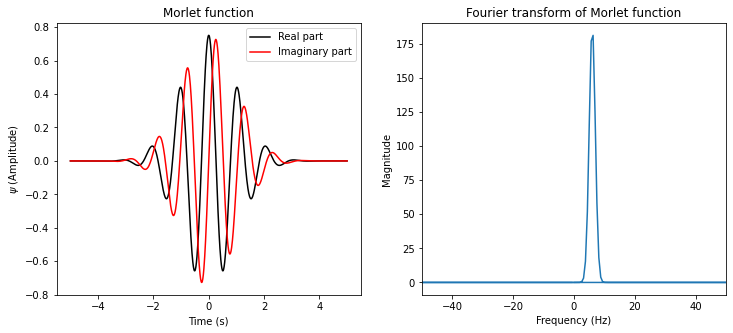
\includegraphics[width=0.8\textwidth]{Morlet_Plot_Python.png}
\caption{ Morlet function in time (real and imaginary) and frequency space.} \label{fig:my_label}
\end{figure}

It is worthy of note that, the Morlet wavelet does not have compact support but has exponential decay. This means that the wavelet function does not go to zero outside a certain range of values, but instead decays exponentially. Regarding the differentiability of the Morlet wavelet, it is not infinitely differentiable. No wavelet with finite support can be infinitely differentiable. This is because, for a wavelet to have compact support, it must be zero outside a certain interval. However, if a function is zero outside an interval, then it cannot have nonzero derivatives of all orders.

Finally, the Morlet wavelet does not come from an MRA (multiresolution analysis). This means that the Morlet wavelet cannot be generated by a series of dilations and translations of a single wavelet function, which is a key feature of MRAs. However, the Morlet wavelet can still be used in wavelet analysis for certain applications, like in our case.



\subsubsection{Phase-Correction in Fourier Space}
After transforming our signal profile into the required wavelet, we can assume a resulting complex wavelet profile in Fourier space as \cite{Hedman_2018}, 
\begin{equation}
    \tilde{X}_{w,i}(a,b) = \Gamma_{i}e^{i\Phi_{i}},
\end{equation}
where $\tilde{X}_{w,i}(a,b)$ is the complex phase-dependent wavelet transformation, $\Gamma_{i}$ is the complex amplitude, $\Phi_{i}$ is the wavelet phase which could be expressed as, $\Phi_{i} = \phi_{r}(r) + |m|(\lambda - \Omega_{p}t) + \phi_{0}$. $\phi_{r}(r)$ is the radiallly dependent portion of the wave-sphase, and for large distances from the resonant radius we can express it as \cite{1984prin.conf..513S},
\begin{equation}
    \phi_{r}(r) = \frac{3|m-1|M_{P}(r - r_{L})^{2}}{4\pi\sigma_{0}r^{4}_{L}}.
\end{equation}
All other parameters maintaining their usual meanings.   

For discrete observations of the longitude $\lambda_{i}$ and epoch time $t_{i}$, the phase parameter can be estmated using the discrete interpretation, $\phi_{i} = |m|[\lambda_{i} - \Omega_{p}t_{i}]$, given specific values of $|m|$ and $\Omega_{p}$. Given a specific wave with defined parameters, the required phase difference becomes $\Phi_{i} - \phi_{i} = \phi_{r}(r) + \phi_{0}$ for all occultations present. Now, the previous steps enables us to redefine the phase corrected wavelet as:
\begin{equation}
    \tilde{X}_{w,\phi,i}(a,b) = \tilde{X}_{w,i}(a,b)e^{i\Phi_{i}} = \Gamma_{i}e^{i(\Phi_{i} - \phi_{i})}.
\end{equation}

Given particular signals with m and $\Omega_{p}$ values, by implication of the phase correction, there will be the same phase for all the occulation profiles present, leading to an average non-zero phase-corrected wavelet:
\begin{equation}
    \langle\tilde{X}_{w,\phi}(a,b)\rangle = \frac{1}{N} \sum_{i=1}^{N}\tilde{X}_{w,\phi,i}(a,b).
\end{equation}

Any signal without similar phase attributes will average to zero, leaving the desired signal in the power of the average phase-corrected wavelet, expressed as,
\begin{equation}
    \mathcal{P}_{\phi}(r,k) = |\langle\tilde{X}_{w,\phi}(a,b)\rangle|^{2} = \left|\frac{1}{N} \sum_{i=1}^{N}\tilde{X}_{w,\phi,i}(a,b)\right|^{2}.
\end{equation}
On the other hand, all other signals will be captured in the average wavelet power,
\begin{equation}
     \bar{\mathcal{P}}(r,k) = \langle|\tilde{X}_{w,\phi}(a,b)|^{2}\rangle = \frac{1}{N} \sum_{i=1}^{N}|\tilde{X}_{w,\phi,i}(a,b)|^{2}.
\end{equation}

To guage how much of the signal is consistent with the assumed m and $\Omega_{p}$, we take the ratio \cite{Hedman_2013}:  $\mathcal{T}_{\phi}(r,k) = \frac{\mathcal{P}_{\phi}(r,k)}{\bar{\mathcal{P}}(r,k)}$ $\forall$ $\mathcal{T}_{\phi}(r,k) \in (0,1)$.








\subsubsection{Wavelet Reconstruction Formula}
For proper reconstruction, we use the average phase-corrected wavelet to create a reconstructed profile with given m, and pattern speed. 

We start by assuming $x_{\phi}\in L^2(\mathbb{R})$, we can reconstruct our signal using the famous Calderon's technique \cite{Caldern1964IntermediateSA}\cite{pereyra2012harmonic}\cite{Roy_2022}\cite{APracticalGuidetoWaveletAnalysis}:
\begin{equation}
x_{\phi}(t) = \frac{1}{C_{\psi}} \int_{0}^{\infty} \int_{-\infty}^{\infty} X_{w,\phi}(a,b) \frac{1}{|a|^{1/2}} \psi\left(\frac{t-b}{a}\right) \frac{db \, da}{a^{2}},
\end{equation}
provided $\psi(t)$ satisfies Calderón's admissibility condition \cite{Caldern1964IntermediateSA}: $C_{\psi} := \int_{-\infty}^{\infty} \frac{|\tilde{\psi}(\xi)|^2}{|\xi|} d\xi < \infty$ and must have a finite energy\cite{Roy_2022}\cite{APracticalGuidetoWaveletAnalysis}: $E_{\psi} = \int_{-\infty}^{\infty} |\psi(t)|^2 dt < \infty$. Here, $\tilde\psi(\omega)$ is the Fourier transform of $\psi(t)$, $\omega = 2\pi \mathcal{\beta}$ is the angular frequency, and $C_{\psi}$ is the admissibility constant. The above condition implies that $\tilde\psi(\omega)$ approaches zero faster than $\omega$ and must not have zero frequency component, $\tilde\psi(0)=0$ \cite{Roy_2022}.






\subsubsection{Alternative Wavelet function}
Recall, $X_{w,\phi}(a,b)=\frac{1}{\sqrt{|a|}}\tilde{X}_{w,\phi}(a,b)$. By direct substitution into equation 5, we have:
\begin{equation} 
x_{\phi}(t) = \frac{1}{C_{\psi}} \int_{0}^{\infty} \int_{-\infty}^{\infty}\frac{\tilde{X}_{w,\phi}(a,b)}{|a|} \psi\left(\frac{t-b}{a}\right) \frac{db \, da}{a^{2}}.
\end{equation}


We can also choose a completely different wavelet function, Morlet's technique, like the Dirac-delta function $\delta\left(\frac{b-t}{a}\right)$, instead of the analysing wavelet \cite{doi:10.1146/annurev.fl.24.010192.002143,Roy_2022}. Here: 
\begin{equation}
    x_{\phi}(t) = \frac{1}{C_{\psi}} \int_{0}^{\infty}\frac{1}{|a|} \left(\int_{-\infty}^{\infty} \tilde{X}_{w,\phi}(a,b)\delta\left(\frac{t-b}{a}\right)db\right)\frac{da}{a^2}
\end{equation}


Recall for a Delta function, $\delta(-x)=\delta(x)$ and $\int_{-\infty}^{\infty}\delta(x-d)f(x) dx=f(d)$.

Using $b=ay$, and working through the double-integral, we have: $\int_{-\infty}^{\infty} \tilde{X}_{w,\phi}(a,b)\delta\left(\frac{t-b}{a}\right)db = a\tilde{X}_{w,\phi}(a,t)$.

By direct substitution into equation 5, we arrive at a simplified single integral for our wavelet reconstruction given as \cite{doi:10.1146/annurev.fl.24.010192.002143,Roy_2022,APracticalGuidetoWaveletAnalysis}:
\begin{equation}
     x_{\phi}(t) = \frac{1}{C_{\delta}} \int_{0}^{\infty}\frac{\tilde{X}_{w,\phi}(a,t)}{|a|}\frac{da}{a}.
\end{equation}
Note: $C_{\psi}=C_{\delta}$, since we reconstructed the Fourier transforms using a Dirac delta function \cite{APracticalGuidetoWaveletAnalysis}.

\subsubsection{Choice of Scale: From Dyadic to Linear Scale}
Since we are working with nonorthogonal wavelet analysis, it is recommendable to use an arbitrary set of scale to build a more complete wavelet reconstruction formula for previous step above \cite{APracticalGuidetoWaveletAnalysis}. To enable us succeed in this case, we assume a variant of the dyadic scales given in \cite{pereyra2012harmonic,APracticalGuidetoWaveletAnalysis}: 
\begin{equation}
    a_{j} =a_{0}2^{j\delta_{j}},
\end{equation}
where, $j=0,1,2,...,J$; $a_{0}$ is the smallest resolvable scale, assumed to be constant for our data. 

Consider the term, $\delta_{j}$, signifying the scaled range of wavelength measurement, intricately linked to the non-dimensional frequency, $\omega_{0}$. We represent this relationship as: 
\begin{equation}
    \delta_{j} = \tilde{\epsilon}\Delta{a}.
\end{equation}
Here, $\delta_{j}$ encapsulates the scaled range, and its dependency on the non-dimensional frequency. This formulation precisely articulates the nuanced connection between $\delta_{j}$ and $\omega_{0}$, contingent upon the boundary condition required for an optimized result, $\tilde{\epsilon} = \sup\{\tilde{\phi} \in \mathbb{R}: 0 < \tilde{\phi} \leq \omega_0\}$, and $\Delta{a}=[a(j),a(j+1)]$, assumed to be constant for our specific signal data. 

First, to linearize the dyadic scale, we take the natural logarithm of equation (45): $\ln a_{j} = \ln a_{0} + j\delta_{j} \ln2$. Now, differentiating the previous equation with respect to the variable, $j$, simply produces the result: $\frac{da_j}{a_j} = \delta_{j} \ln2$. Note here that, $dj = (j+1)-j= 1$ for discrete case. 

Finally, we substitute the result of the latest differential equation into the equation (44), and express the total results discretely, it results to the following:
\begin{equation}
x_{\phi}(t) = \frac{\tilde{\epsilon}\Delta a\ln 2}{C_{\delta}} \sum_{j=0}^{J} \frac{\tilde{X}_{w,\phi}(a_{j},t)}{|a_{j}|}
\end{equation}

Practically, our reconstructed time series can be taken as the sum
of the real part of the wavelet transform over all scales \cite{APracticalGuidetoWaveletAnalysis}. To ensure optimal computational efficiency, we meticulously normalize and fine-tune the aforementioned reconstruction. Our final expression for achieving peak performance and accuracy becomes: 
\begin{equation}
 x_{\alpha,\phi}(t) = \tilde{\epsilon}\Delta a\lfloor \alpha \rfloor\sum_{j=0}^{J} \frac{\Re (\tilde{X}_{w,\phi}(a_{j},t))}{|a_{j}|}
\end{equation}
where $\alpha=\frac{ln2}{C_{\delta}\psi(0)}$, $C_{\delta}= 0.776$ \cite{APracticalGuidetoWaveletAnalysis}; $\psi(0)=\pi^{-1/4}$ \cite{APracticalGuidetoWaveletAnalysis}.
$x_{\alpha,\phi}(t)$ is the final, reconstructed phase-corrected form of $x(t)$. We will use this expression in our Python computational analysis in the section below. 

\subsubsection{Sample Reconstruction}
In a bid to verify the authenticity of our customized wavelet reconstruction formula, we assume a noisy signal given by the equation:
\begin{equation}
   x(t) = 5\sin\left(\frac{2\pi t}{0.02} + 10\right) + 3\sin\left(\frac{2 \pi t}{0.05}\right)
\end{equation}
where $t = \texttt{np.linspace(0, 1, nrx=1000)}$ in Python computations, $\Delta a=1$, $\tilde{\epsilon}=\tilde{\phi} = 6.0$, and other constants having the same value as defined previously.

%We are going to compare our plot with that obtained using the PyWavelet Python library, below.

\begin{figure}[h]
\centering 
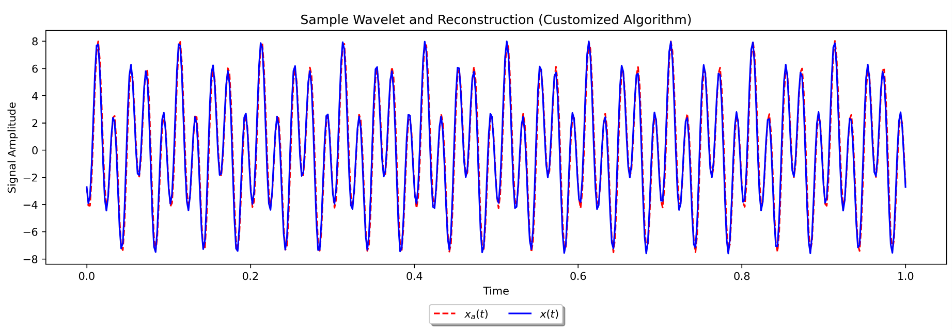
\includegraphics[width=0.8\textwidth]{Python_Wavelet_Transform_Plot_Combined.png} 
\caption{Sample Wavelet Plots (Main and Reconstructed Signals)} \label{fig:my_label}
\end{figure}


%\begin{table}[h]
%\centering
%\begin{tabularx}{0.8\textwidth} { 
 % | >{\raggedright\arraybackslash}X 
  %| >{\centering\arraybackslash}X 
  %| >{\raggedleft\arraybackslash}X | }
 %\hline
 %Method & Correction Factor & Flexibility \\
 %\hline
 %Customized Algorithm  & 1.0130  & High  \\
%\hline
%PyWavelet Package  & 1.0155  & Limited  \\
%\hline
%Scipy.signal Package  & ---  & No Algorithm  \\
%\hline
%\end{tabularx}
%\caption{Comparison of correction factor and flexibility between different methods (Figure 5).}
%\label{table:comparison}
%\end{table}

\begin{table}[h]
\centering
\begin{tabularx}{0.8\textwidth} { 
  | >{\raggedright\arraybackslash}X 
  | >{\centering\arraybackslash}X 
  | >{\raggedleft\arraybackslash}X | }
 \hline
 Method & Correction Factor & Flexibility \\
 \hline
 Customized Algorithm  & 1.0130  & High  \\
\hline
\end{tabularx}
\caption{Outline of properties for Customized algorithm (Figure 7).}
\label{table:comparison}
\end{table}

From the plots and table, the customized algorithm has the lowest correction factor and a high flexibility in terms of varying the parameters for accurate results. This factor represents how much the wavelet transform has modified the original signal in terms of relative magnitude. Specifically, a factor greater than 1 means that the modified signal has larger amplitude than the original signal, while a factor less than 1 means that the modified signal has smaller amplitude than the original signal. The next section discusses the main results of using our customized codes on real wavelet data from the recent Cassini missions (2004 to 2017).  

%......................................................................................
\subsection{Implementation Routine}
\subsubsection{Data acquisition}
To analyze the amplitude of spiral density waves in Saturn's C ring, we first obtained VIMS(Visual and Infrared Mapping Spectrometer) data on the C-ring structure, using Fourier analysis to break down the ring structure in terms of its individual frequency (wavelength) components. Specifically, we used data from the Cassini spacecraft, with epoch of 1o years, to obtain measurements of the density waves in the rings. The data consists of images of the rings taken by the spacecraft.
\subsubsection{Image processing}
To apply Fourier transforms to the spiral density waves in Saturn's rings, we will first need to convert the set of images of the visual infrared and mapping spectrograph occultations for the ring structure, into a set of brightness values with higher values corresponding to regions of higher particle density, and vice-versa. The processed images contain information about the density waves, such as the location and shape of the waves in the images, as well as their amplitudes.
\subsubsection{Fourier transform}
We will first use the Continuous Wavelet Transform (CWT) algorithm to transform the time series of the amplitude measurements into the frequency domain. This will allow us to also perform phase correction of the distorted signals, owing to blockage or distortion by the planetary body.
\subsubsection{Phase-Correction Algorithm In Fourier Space}
In general, phase-correction is commonly used in signal processing to correct for phase distortions or misalignments that may have occurred during data acquisition or processing. In the context of planetary science or planetary seismology, phase correction may be used to correct for phase shifts or time delays in seismic signals caused by the propagation of seismic waves through a planetary body with a complex internal structure, like Saturn. For example, in the case of an occultation geometry, where a spacecraft passes behind a planet or moon and its signal is blocked or distorted by the planetary body, the seismic signals received by the spacecraft may be affected by the planet's internal structure, which can introduce phase shifts or time delays. By applying phase correction to the wavelet transform of the seismic signal, it may be possible to remove or mitigate some of these phase shifts or time delays, allowing for more accurate analysis and interpretation of the seismic data.
\subsubsection{Signal Reconstruction}
Here, we average the resulting signals present in the whole wave occultation, after the phase-corrected has been performed. We will utilize our customized algorithm in Python computing language to recover our signals.
%\subsection{Analysis}
%We will analyse the results of the reconstructed Fourier transform to gain insights into the underlying physics of the system. This will involve comparing the results from different locations in the ring system and identifying any patterns or correlations with Saturn's interior dynamics.

\subsection{Main Signal Versus Reconstructed Signal}
Following the required implementations for the wavelet algorithms in Python, and using the Morlet wavelet as the required mother wavelet, the following plots show the comparisms for a particular case using a sample Satellite resonance spiral density wave, \textbf{Atlas 2:1}, as a case-study. 


\textbf{A. Average Wavelet Power:}
The average wavelet power is a measure of the energy or power of a signal at different scales and positions in both time and frequency domains. In this context, it is calculated by taking the square root of the sum of the squares of both components of our data arrays along a specified axis. This could be a representation of the overall power of the sample wavelet signal. The image plot visualizes the distribution of wavelet power across spatial wavelengths and radii. The x-axis typically represents spatial wavelengths (1/km), and the y-axis represents radii (typically in 1000 km units).

\textbf{B. Power of Average Phase-Corrected Wavelet:}
This variable represents the power of the average phase-corrected wavelet. Phase-corrected wavelets are often used to enhance specific features or remove noise in a signal, as explained previously. This represents the power after applying phase correction. The image plot displays the distribution of power for the phase-corrected wavelet, similar to the first plot.

\textbf{C. Power Ratio:}
This variable represents the power ratio, which is calculated by dividing Power of Average Phase-Corrected Wavelet by Average Wavelet Power. It indicates how the power of the phase-corrected wavelet compares to the overall wavelet power. The image plot provides a visual representation of this power ratio, showing areas where the phase correction enhances or reduces the power relative to the average wavelet power.

These plots help visualize and analyze the distribution of power and the impact of phase correction in the context of wavelet analysis. They can be valuable for identifying patterns or features in the data and understanding the effectiveness of phase correction techniques in signal processing (more to come below).

\vspace{0.5pt}

\textbf{Note:}
The \textbf{'plt.imshow'} function is used to create these image plots. The \textbf{'vmin'} and \textbf{'vmax'} parameters control the color scale, and the \textbf{'extent'} parameter specifies the range of values for the x and y axes. The \textbf{'plt.xlabel'} and \textbf{'plt.ylabel'} functions set labels for the x and y axes of each plot.

\begin{figure}[h]
\centering 
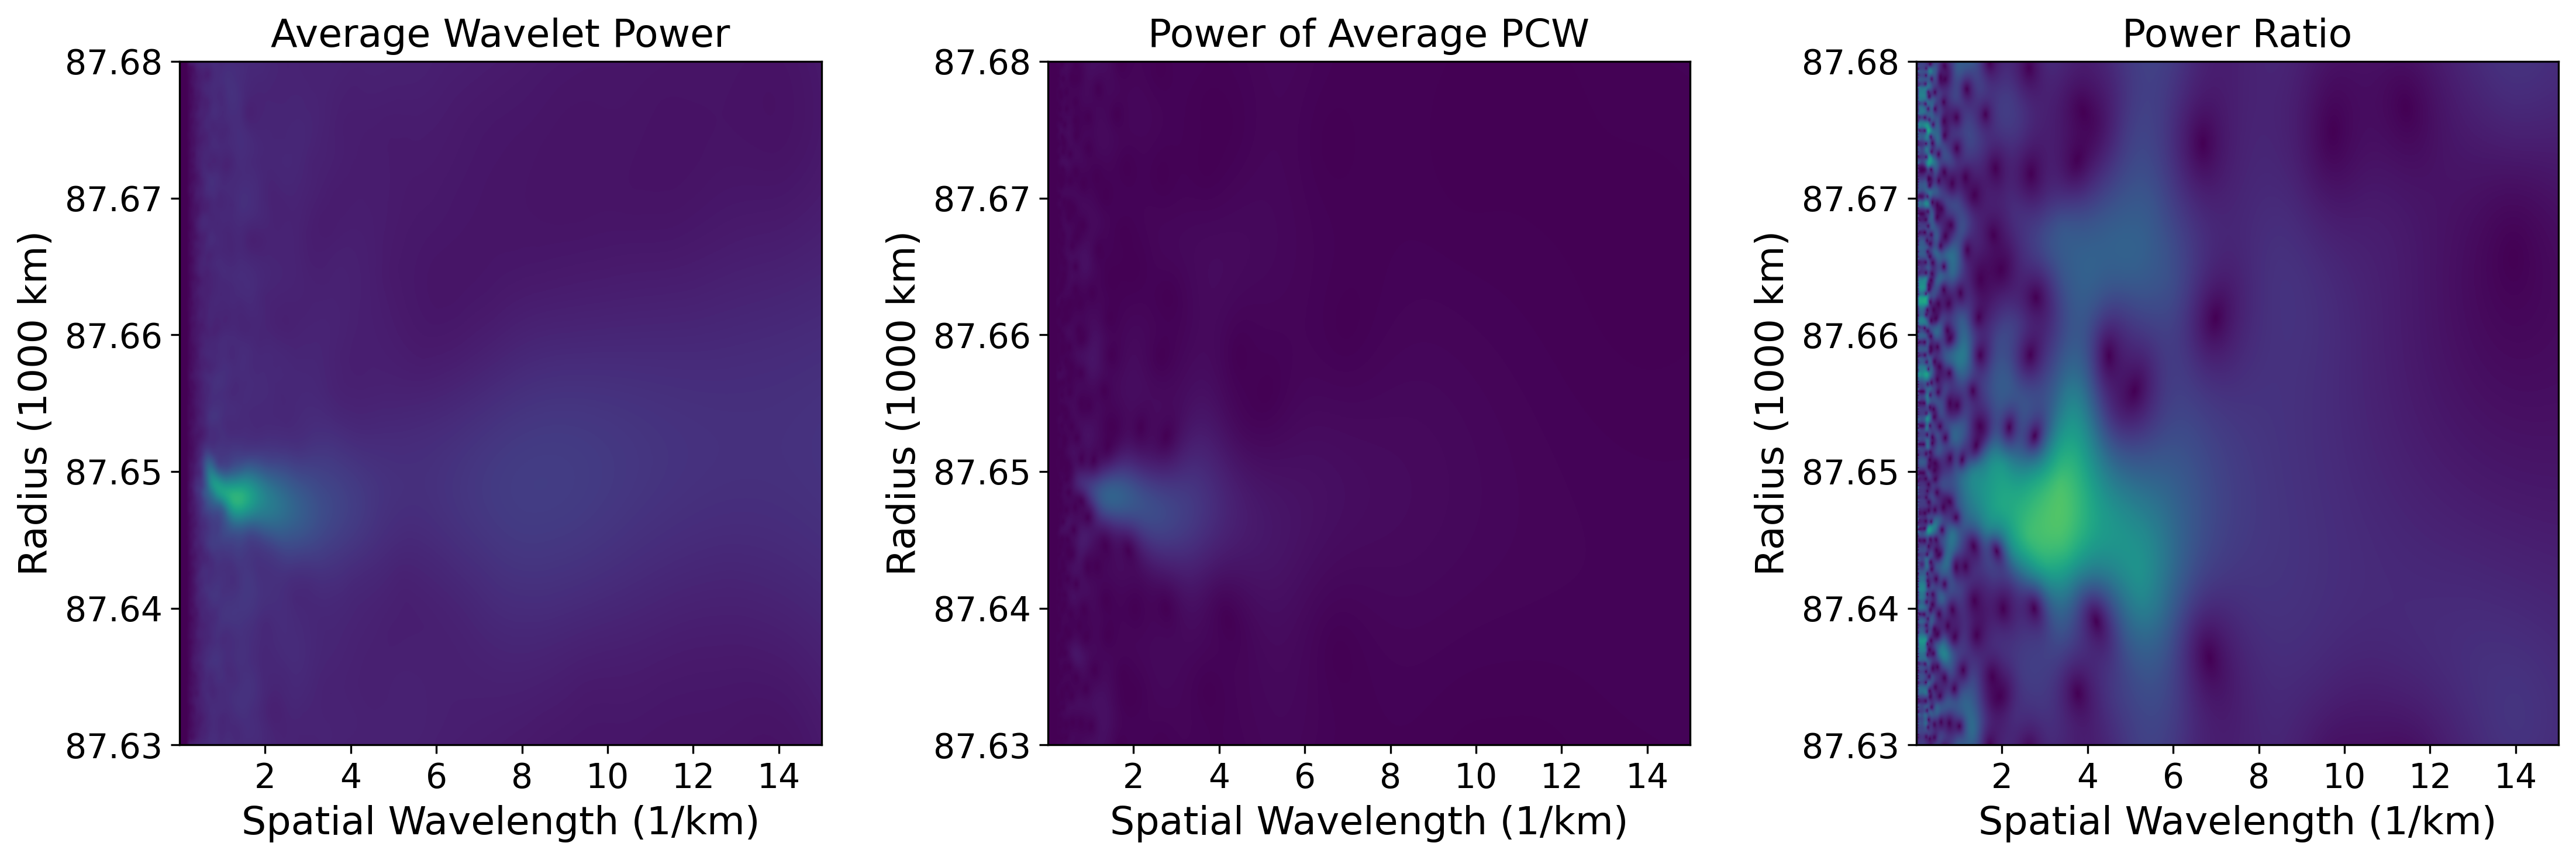
\includegraphics[width=1.0\textwidth]{power_ratio_plotw87.png} 
\caption{Plots for the Power Spectrum of the Satellite resonance wavelet signal, \textbf{Atlas 2:1}, reveal that it falls within the radial range of 87.64 - 87.65 (in units of 1000 kilometers) and exhibits a spatial wavelength between approximately 1 and 9 (per kilometer).} \label{fig:my_label}
\end{figure}


A final comparison is presented in Figure 9, showcasing reconstructed occultation profiles for this specific wavelet. The top plot (orange legend) represents the average background density variations associated with the signal. The initial reconstructed average wavelet (blue legend) is a cumulative representation of the occultation profiles contained within the wavelet data. The second reconstructed wavelet plot (green legend) is the first reconstructed average wavelet, which has been normalized to the background surface density in the region of Saturn's C-ring. It is evident that the wavelet reconstruction techniques perform exceptionally well in this particular case.

\begin{figure}
\centering 
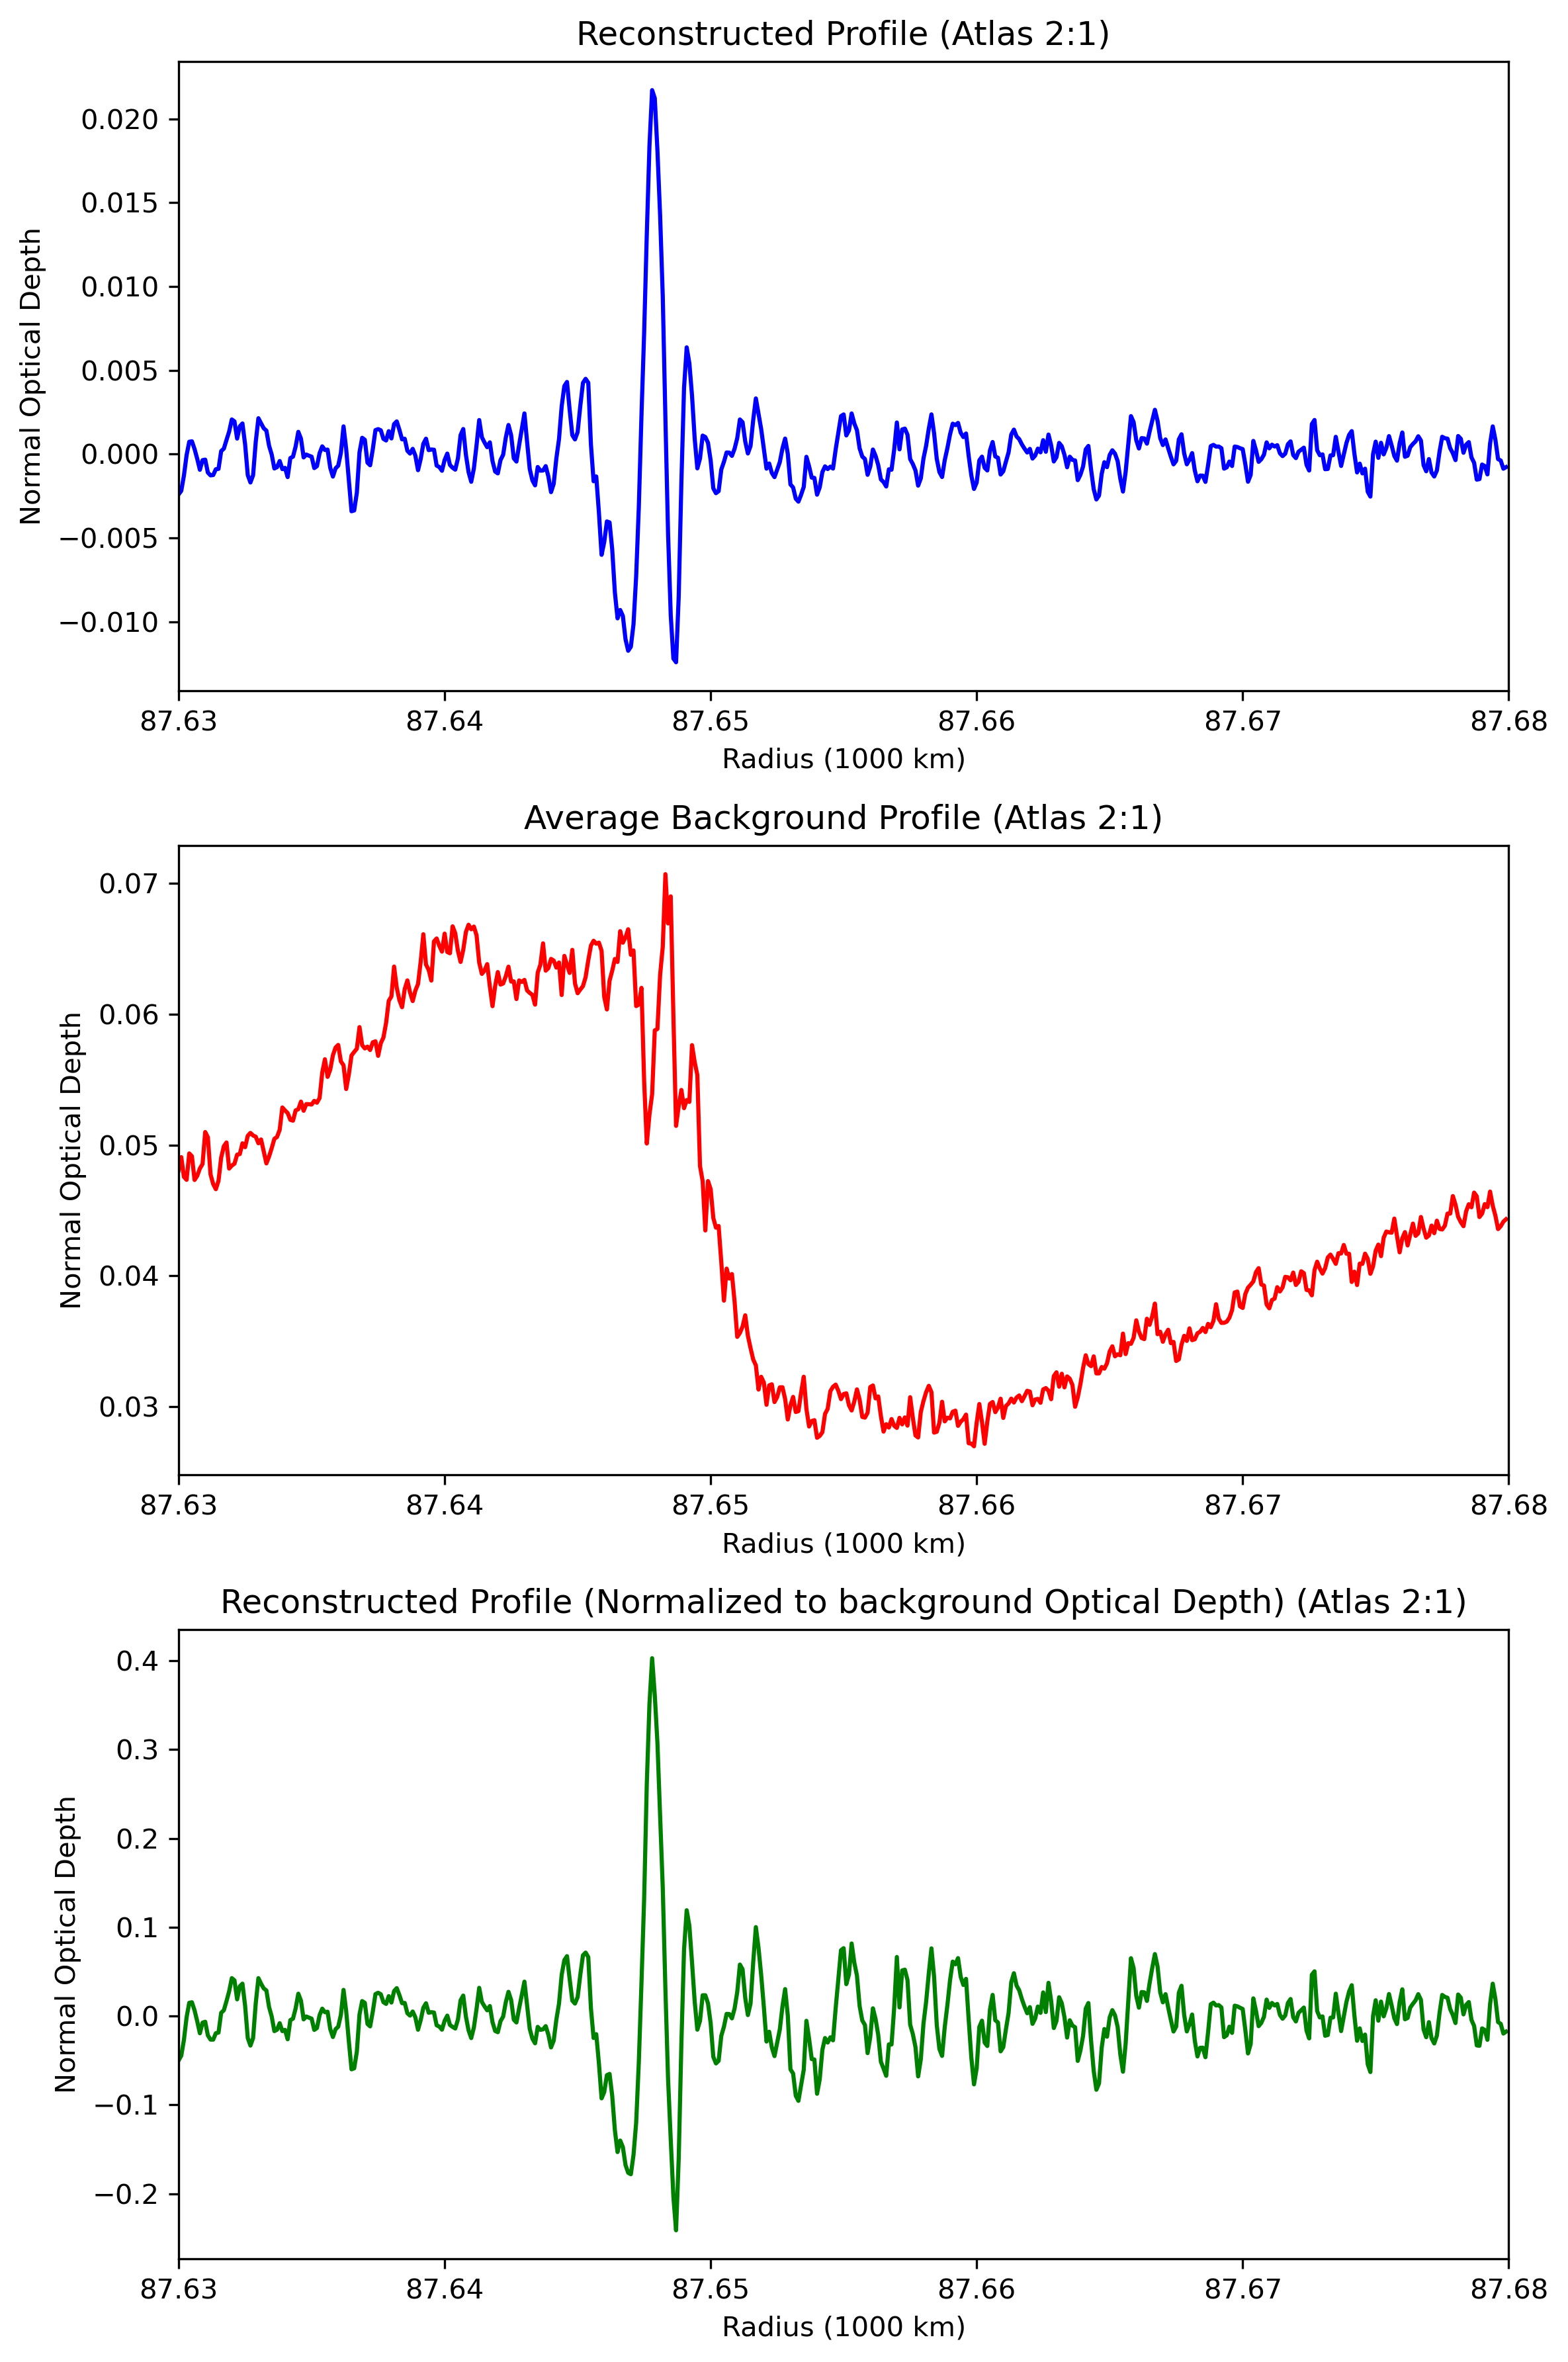
\includegraphics[width=0.8\textwidth]{combinedprofiles_atlas21.png}
\caption{A combined profiles for wavelet occultations for the Atlas 2:1 Satellite resonance.} \label{fig:my_label}
\end{figure}


%...............................................................................

\textbf{Final Note:}
The phase-correction algorithm applies phase shifts to the wavelet transform and then computes the average phase-corrected wavelets for each pattern speed. The captions describe two wave profile plots. In the first plot, the Normal Optical Depth is shown with a vertical offset, without phase correction. This plot highlights noisy wave profiles that are not properly aligned with expected results. In the second plot, the Normal Optical Depth is again displayed with a vertical offset, but this time with phase correction. Here, the wave profiles are less noisy and exhibit better alignment, as expected.

%The explained algorithm has led to significant findings regarding the behavior of waves in Saturn's rings. In particular, the wave analysed has proven to be strongly impacted by the planet's internal structure, including its rotation rate and density distribution, and not by any of Saturn's moons \cite{FRENCH2019599}\cite{Hedman_2018}. The study also discovered new information about the properties of these waves, such as the slightly changing positions of their amplitudes and some dips located along the regions of the detected waves, as evidenced in the plots of their optical depth profiles versus the radial distance \cite{BORDERIES1986522}. 

%\begin{figure}[h]
%\centering
%\begin{subfigure}[b]{1.1\textwidth}
 %  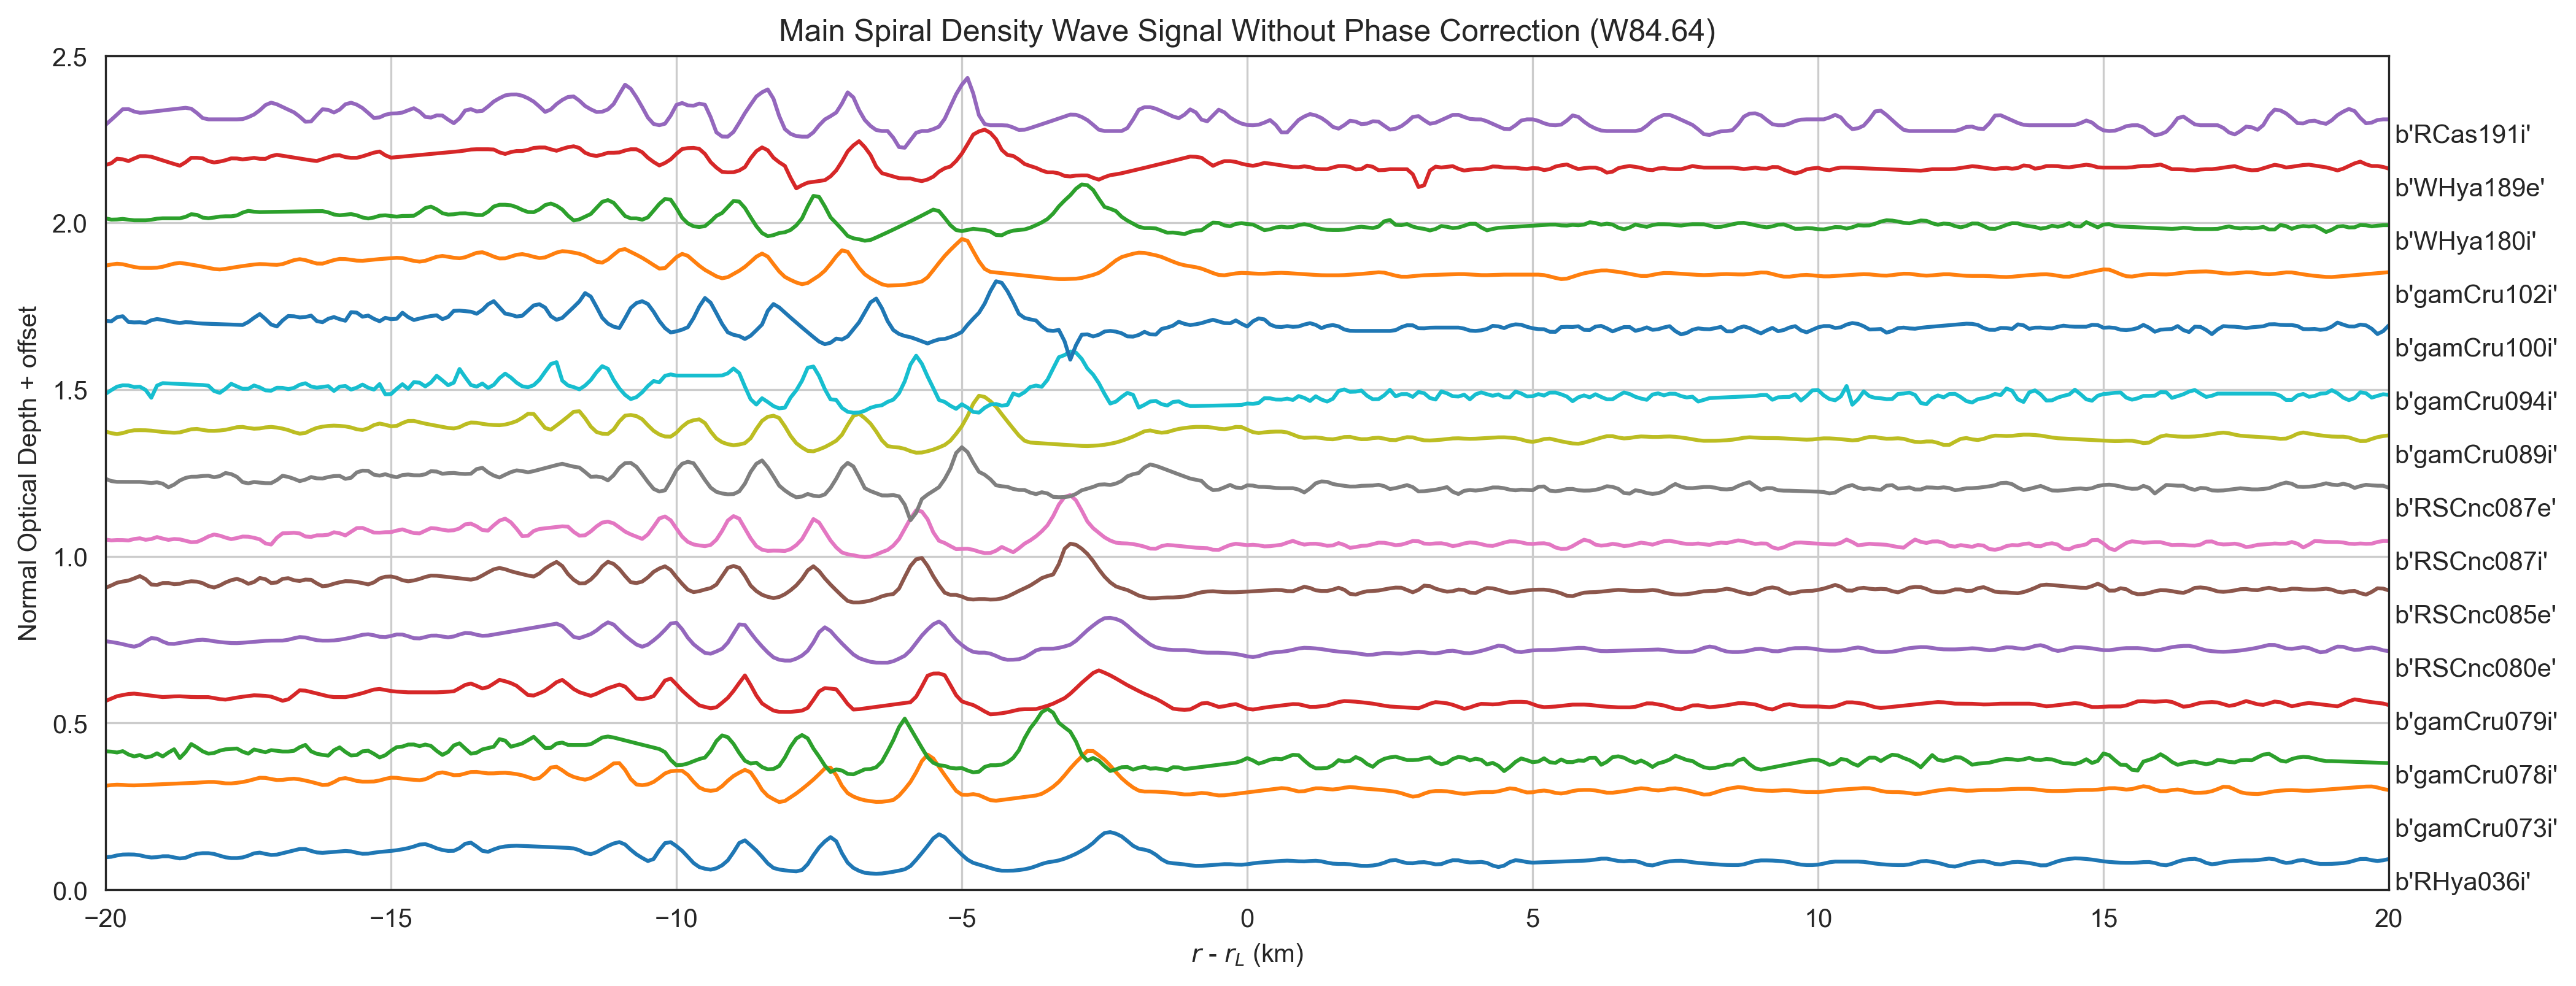
\includegraphics[width=0.9\linewidth]{Main_Main.png}
 %  \caption{}
  % \label{fig:Ng1} 
%\end{subfigure}
%\begin{subfigure}[b]{1.1\textwidth}
 %  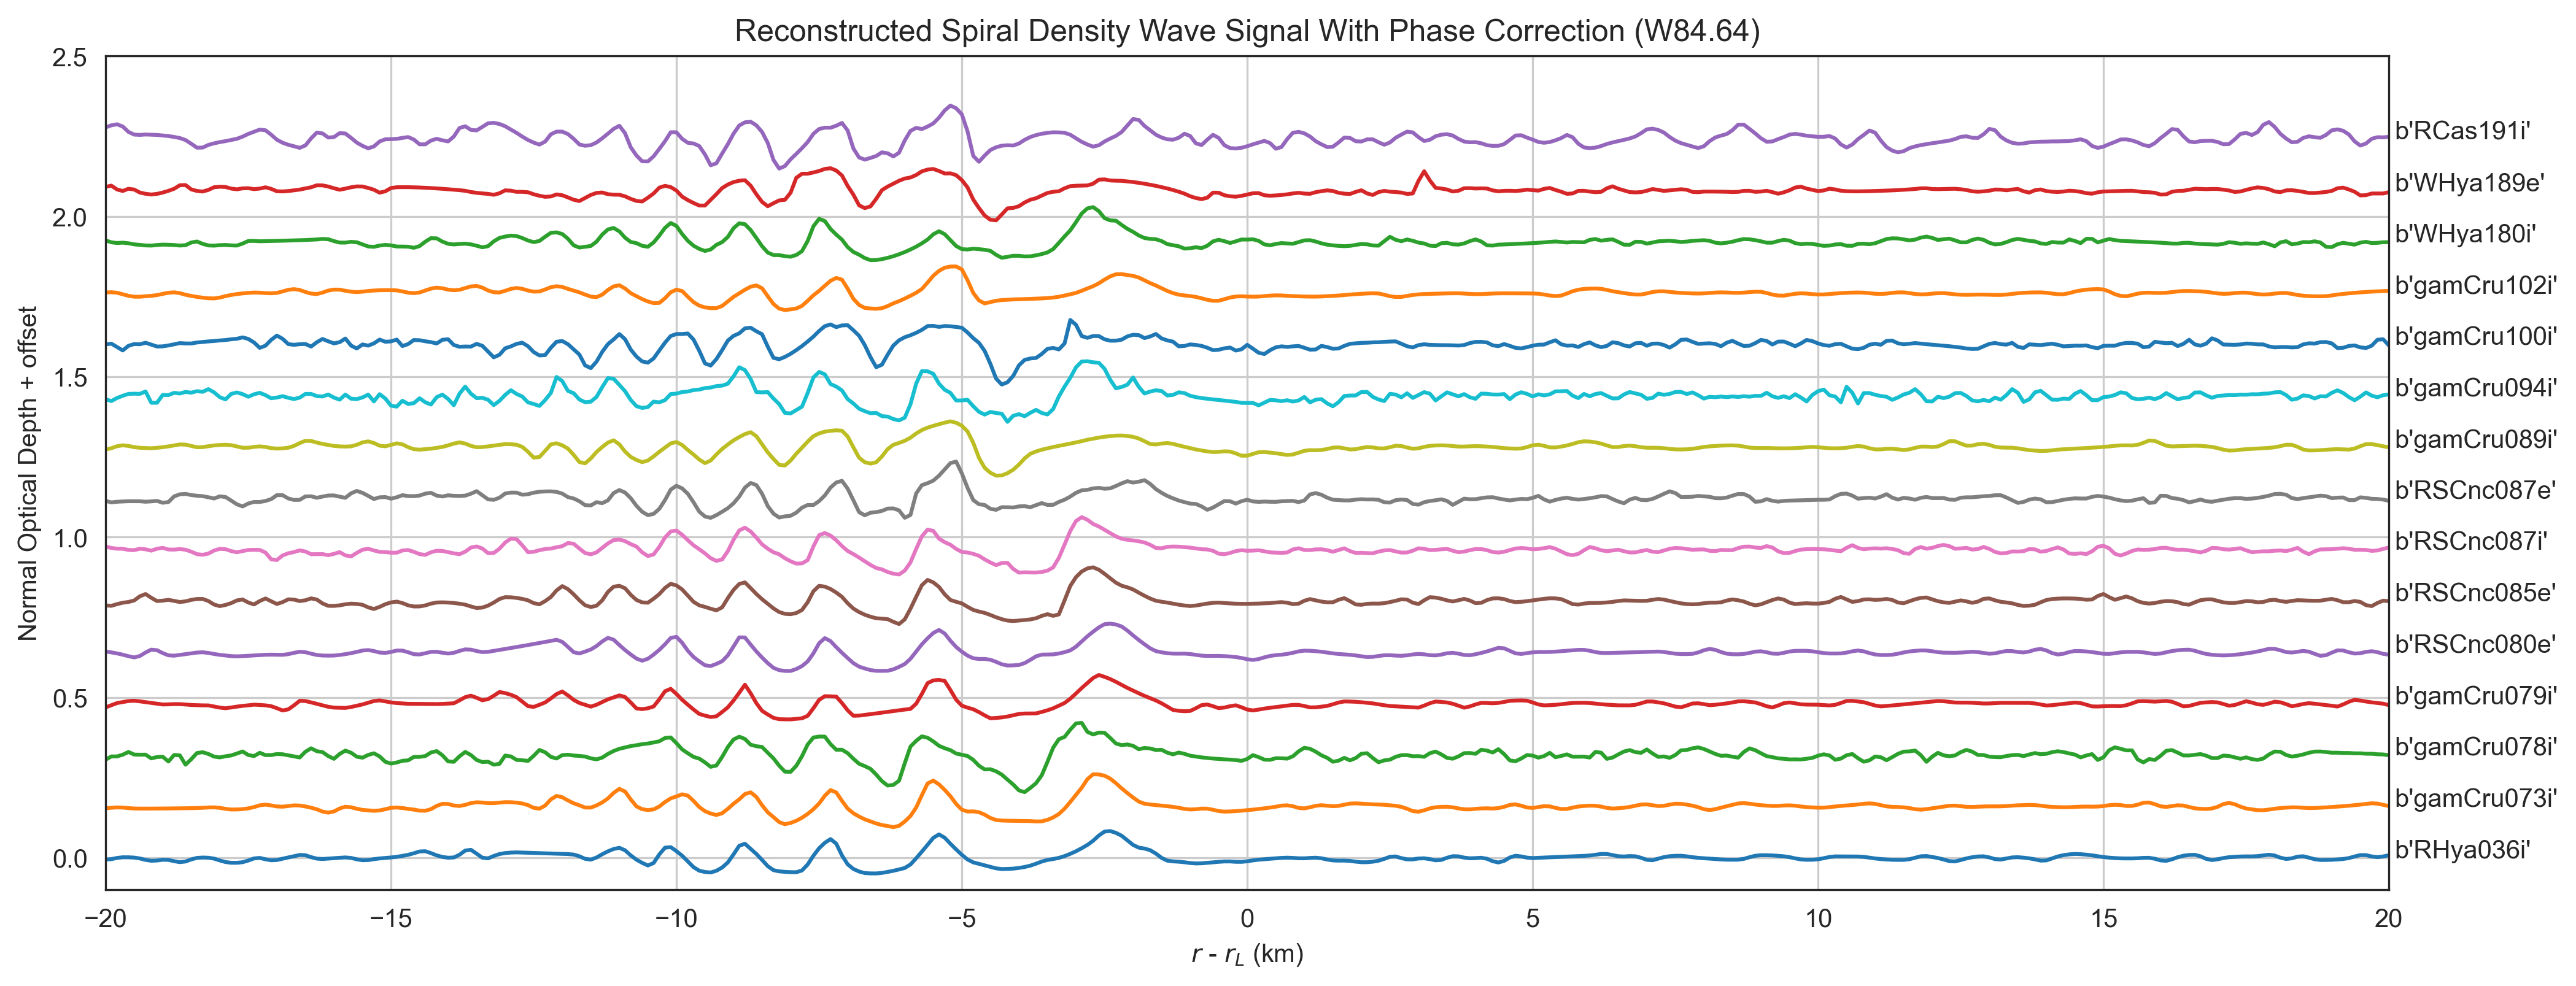
\includegraphics[width=0.9\linewidth]{Reconstructed_Main.png}
  % \caption{}
  % \label{fig:Ng2}
%\end{subfigure}
%\caption[Caption for Two Wave Profile Plots]{(a) Plot of the Normal Optical Depth (with vertical offset) for the wave profile (without phase correction). In this plot, the wave profiles exhibit noise and lack proper alignment. (b) Plot of the Normal Optical Depth (with vertical offset) for the wave profile (with phase correction). Here, the profiles appear less noisy and are mostly well-aligned.}
%\end{figure}


\begin{figure}[h]
    \centering
    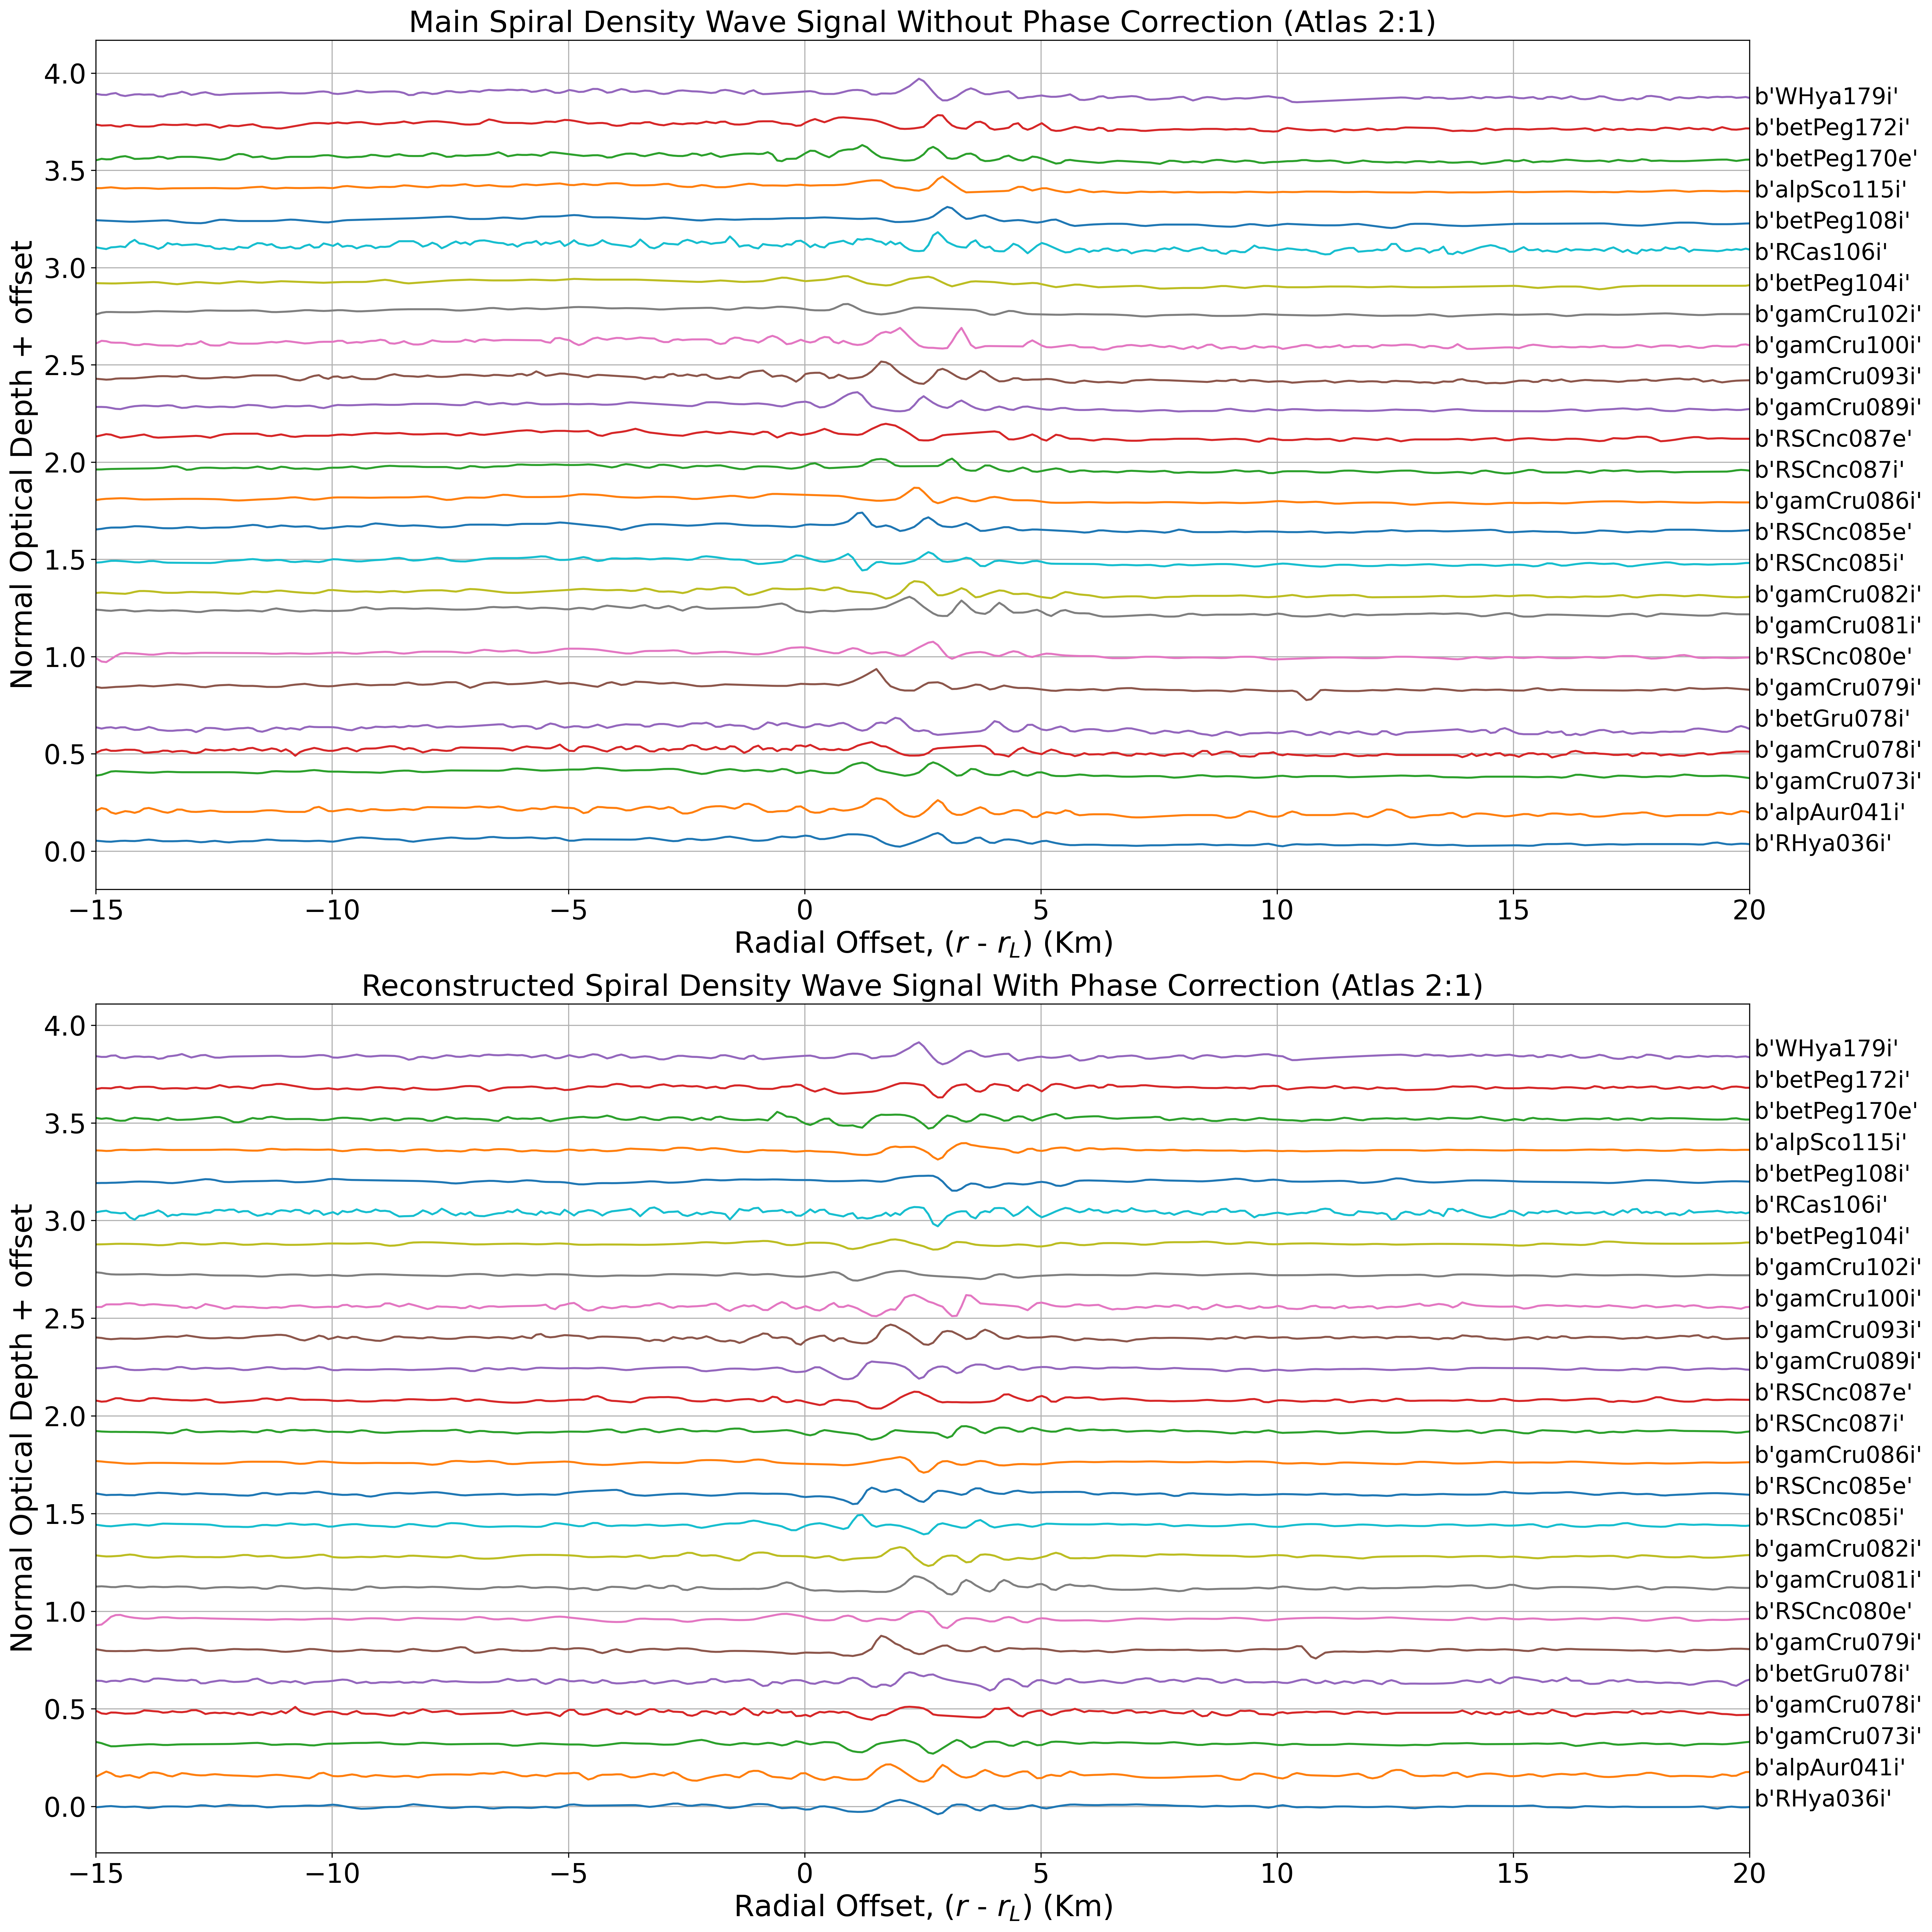
\includegraphics[width=0.5\linewidth]{main_reconstructed_atlas21.png}
    \caption{[Upper Panel]: Plot of the Normal Optical Depth (with vertical offset) for the wave profile occultations (without phase correction). In this plot, the wave profiles exhibit noise and lack proper alignment in phase. [Lower Panel]: Plot of the Normal Optical Depth (with vertical offset) for the wave profile occultations (with phase correction). Here, the profiles appear less noisy and are mostly well-aligned in phase.}
    \label{fig:enter-label}
\end{figure}


\subsection{Wave-Fitting Routine}
In the process of gleaning the required information from the reconstructed signals, some pertinent parameters come to mind. 

Firstly, the surface mass density, $\sigma_{0}$, which represents the mass distribution across the section of the ring, around the region of the detected wave. It is a measure of the density of matter present in the wave. The wave-fitting process can be best achieved by determining the value of $\sigma_{0}$ that best fits the observed data. Secondly, viscosity, $\nu$, is associated with the region of the ring where the spiral density wave is located. It measures the resistance to the flow of matter within that region of the ring. Thirdly, the normal-mode amplitude coefficient, $C^{'}_{lmn}$, simply represents the spherical harmonic coefficient for Saturn's gravitational field, which could be interpreted as the amplitude of the planetary oscillation responsible for exciting spiral density waves across Saturn's (C)-ring(s). Thus, when considering the case where $n=0$, the amplitude coefficient simplifies to $C^{'}_{lmn}$, which also means the modes are fundamental in nature (as described above). In subsequent sections below, we present our steps for the wave-fitting routine.

\subsubsection{Surface Mass Density, $\sigma_{0}$}
Recall equation (6), $\xi = \left[\frac{3|m-1|\Omega_{L}^{2}r_{L}}{4\pi G \sigma_{0}}\right]^{\frac{1}{2}}\left(\frac{r-r_{L}}{r_{L}}\right)$. Let the coefficients of $(r-r_{L})$ be $\frac{1}{x_{f}}$. This implies:
\begin{equation}
 \frac{1}{x_{f}} = \left[\frac{3|m-1|\Omega_{L}^{2}r_{L}}{4\pi G \sigma_{0}}\right]^{\frac{1}{2}}\left(\frac{1}{r_{L}}\right),
\end{equation}
where $\Omega_{L}^{2} = \frac{G M_{P}}{r_{L}^{3}}$. When we substitute for $\Omega_{L}$, square both sides of the equation and perform further simplification, we could express $\sigma_{0}$ in terms of other parameters as:
\begin{equation}
 \sigma_{0} = \frac{3 |m-1| M_{P}x_{f}^{2}}{4\pi r_{L}^{4}}
\end{equation}

Here, $m$ is the azimuthal order of the wave signal. $x_{f}$ is the winding parameter from the Python Wave-fitting routine, measured in $Km$.  $r_{L}$ is the resonant radius of the wave-signal.  $M_{P}$ is the mass of Saturn ($5.6846 \times 10^{26}$ Kg). \textbf{Note:} The S.I. Unit of $\sigma_{0}$ corresponds with the standard measurement in $Kgm^{-2}$.


\subsubsection{Mass Extinction Coefficient, $\kappa$}

We can estimate the value of $\kappa$ by utilizing the surface mass density $\sigma_{0}$ and the average value of the optical depth profiles for the wave signals, denoted as $\tau_{av}$, following the formulation provided in the equation below:

\begin{equation}
    \kappa_{av} = \frac{\tau_{av}}{\sigma_{0}}.
\end{equation}

Typically, the normal optical depth is determined based on the slant angle, $B$, of the observed beam of light concerning the plane of the planetary ring. This computation is detailed on page 378 of Chapter 13 in Dougherty's work \cite{Dougherty2009SaturnFC}:

\begin{equation}
    \tau_{n} = \mu_{n} \ln\left(\frac{I_{0}}{I - b^{*}}\right),
\end{equation}

where $I$ represents the measured intensity of the occulted beam, $I_{0}$ stands for the unocculted intensity, $b^{*}$ accounts for any background signal, and $\mu_{n} = |\sin(B)|$. This formulation assumes negligible effects from self-gravity wakes while offering a consistent methodology for presenting occultation profiles. According to studies \cite{2011Icar..216..292B, ctx2241679689740001851}, the mass extinction coefficient for a differential particle size distribution, defined as $n(a^{*}) = n_{0}(\frac{a_{0}}{a^{*}})^{q}$ with $a^{*} \in [a_{min},a_{max}]$, can be represented as follows:

\begin{equation}
    \kappa = \frac{3(4 - q)}{4(3 - q)}\left(\frac{a_{max}^{3-q} - a_{min}^{3-q}}{a_{max}^{4-q} - a_{min}^{4-q}}\right)\frac{1}{\rho},
\end{equation}

where $\rho$ denotes the particle mass density. The estimation of the mass extinction coefficient at $q\approx3.1$ for the C-ring suggests an inverse relationship with the upper limit for the particle dimension \cite{2011Icar..216..292B}. Assuming uniform particles along the plane of the ring with a radius $R$ and density $\rho$, the mass extinction coefficient can be expressed as:

\begin{equation}
    \kappa = \frac{3}{4\rho R},
\end{equation}

consistent with initial observations indicating that larger opacities are associated with a higher proportion of smaller particles \cite{SHU1983185}.


\subsubsection{Viscosity, $\nu$}
Assuming the damping phenomenon is insufficient to allow several wavecycles, we can estimate the ring section's kinematic viscosity, $\nu$, as in the case \cite{GOLDREICH1978240,1984prin.conf..513S,Tiscareno_2007}:
\begin{equation}
    \nu = \frac{9}{7\Omega_{L}\xi_{D}^{3}}\left(\frac{r_{L}}{\mathcal{D}_{L}}\right)^{1/2}(2\pi G \sigma_{0})^{3/2}
\end{equation}
 
 Where $\mathcal{D}_{L}$ = $3|m-1|\Omega_{L}^{2} + J_{2}(\frac{r_{s}}{r_{L}})^{2}[\frac{21}{2}-\frac{9}{2}|m-1|]\Omega_{L}^{2}$. The second term is only applicable as a correction factor for cases when $m \neq 1$.

Making substitutions for $\Omega_{L}$ and simplifying this equation, the viscosity becomes: 
\begin{equation}
    \nu = \frac{9}{7 x_{D}^{3}}(\frac{Gr_{L}^{7}}{M_{P}^{2}d_{L}})^{\frac{1}{2}}(2\pi\sigma_{0})^{\frac{3}{2}}
\end{equation}
 Where $d_{L}$ = $3|m-1| + J_{2}(\frac{r_{s}}{r_{L}})^{2}[\frac{21}{2}-\frac{9}{2}|m-1|]$. $x_{D}$ is the same as $\xi_{D}$, the dimensionless damping Parameter. The new term is required for the wave-fitting routine, as we shall see in subsequent procedures. $G = 6.674 \times 10^{-11}m^{3} Kg^{-1} s^{-2}$. $r_{s} = 60330$Km (Equatorial radius for Saturn). $J_{2} = 0.01629$ (For Saturn). \textbf{Note:} The S.I. Unit of $\nu$ corresponds with measurements in $m^{2}s^{-1}$.


\subsubsection{Saturn's Normal-mode Amplitude Calculations, $C_{lm0}^{'}$}
From \cite{Marley1993PlanetaryAM} and \cite{Zharkov1985ThePO}, we express the total gravitational potential of a planet as: \begin{equation}
    \Phi = \Phi_{0} + \Phi{'}
\end{equation}
Here, $\Phi_{0}$ = Unperturbed gravitational potential, given as: 
\begin{equation}
\Phi_{0} = \frac{GM}{r}\left\{1 - \sum_{l=1}^{\infty}\left(\frac{a}{r}\right)^{l}J_{l}P_{l}(\cos \theta) + \sum_{l=1}^{\infty}\sum_{m=1}^{l}\left(\frac{a}{r}\right)^{l}P_{l}^{m}(\cos \theta)[C_{lm}(\cos m\phi) + S_{lm}(\sin m\phi)]\right\}
\end{equation}

From \cite{Marley1993PlanetaryAM}, Saturn is a fluid planet in hydrostatic equilibrium, and hence there should be no permanent non-axisymmetric terms in the potential. This implies that $C_{lm}$ and $S_{lm}$ are presumed zero for Saturn.

By reason of the above-mentioned statement, we use $\Phi{'}$ = $\Phi{'}(t)$, time variable gravitational potential (caused by the time-variable density perturbations within Saturn). 

From \cite{Marley1993PlanetaryAM} \cite{Zharkov1985ThePO}, we have:
\begin{equation}
\Phi{'}(t) = \frac{GM}{r}\sum_{n=0}^{\infty}\left\{ - \sum_{l=2}^{\infty}\left(\frac{a}{r}\right)^{l}J_{ln}^{'}P_{l}(\cos \theta) + \sum_{l=2}^{\infty}\sum_{m=-l}^{l}\left(\frac{a}{r}\right)^{l}P_{l}^{m}(\cos \theta)[C_{lmn}^{'}(\cos m\phi) + S_{lmn}^{'}(\sin m\phi)]\right\}
\end{equation}
Note: $l$ = Angular degrees of the wave signals. $a$ = Equatorial radius of Saturn. $n$ = The mode of a particular wave signal (f-mode, $n$ = 0). 


Using the choice of phase, $\phi$ = 0 (is the azimuthal angle \cite{A’Hearn_2022}), $\cos m\phi$ = 1, and $\sin m\phi$ = 0, the equation becomes:
\begin{equation}
\Phi{'}(t) = \frac{GM}{r}\sum_{n=0}^{\infty}\left\{ - \sum_{l=2}^{\infty}\left(\frac{a}{r}\right)^{l}J_{ln}^{'}P_{l}(\cos \theta) + \sum_{l=2}^{\infty}\sum_{m=-l}^{l}\left(\frac{a}{r}\right)^{l}P_{l}^{m}(\cos \theta)C_{lmn}^{'}\right\}
\end{equation}

Since the wave signals have certain numbers of spiral arms, associated with the azimuthal orders of the corresponding planetary oscillations (that is, $m \neq 0$ for the case of non-axisymmetric oscillations), the $J_{ln}^{'}$ component is assumed negligible ($J_{ln}^{'}\approx 0$). The new expression becomes: 
\begin{equation}
\Phi{'}(t) = \frac{GM}{r}\sum_{n=0}^{\infty}\left\{\sum_{l=2}^{\infty}\sum_{m=-l}^{l}\left(\frac{a}{r}\right)^{l}P_{l}^{m}(\cos \theta)C_{lmn}^{'}\right\}
\end{equation}

Recall, we are considering wave signals that are assumed to mostly be from fundamental modes ($n$=0): 
\begin{equation}
\Phi{'}(t) = \frac{GM}{r}\left\{\sum_{l=2}^{\infty}\sum_{m=-l}^{l}\left(\frac{a}{r}\right)^{l}P_{l}^{m}(\cos \theta)C_{lm0}^{'}\right\}
\end{equation}


For understanding the angles, $\theta$ (the colatitude), we are evaluating the potential in the rings, which are at the planet’s equator plane, and taken to be at $90^{o}$ to the (imaginary) vertical axis passing through the center of the planet, Saturn [M. Hedman and V. Afigbo, personal discussions (June, 2022), additional information from \cite{Mankovich_2019}]. We take $\mu = \cos\theta = 0$, and the new equation becomes: 

\begin{equation}
\Phi{'}(t) = \frac{GM}{r}\left\{\sum_{l=2}^{\infty}\sum_{m=-l}^{l}\left(\frac{a}{r}\right)^{l}P_{l}^{m}(\mu)C_{lm0}^{'}\right\},
\end{equation}
where r is the radius \cite{A’Hearn_2022}.

Since we are considering fully normalized gravitational harmonic coefficients, we need to use the fully normalized Associated Legendre Polynomial functions. Considering the orthonormalized harmonics that are commonly used in
the seismology community \cite{Jekeli2007PotentialTA}\cite{2015JASS...32..247S}\cite{https://doi.org/10.1029/2018GC007529}, and using only $|m| \neq 0$ cases, this implies, $P_{l}^{|m|} (\mu) \rightarrow \bar{P}_{l}^{|m|} (\mu)$, where:

\begin{equation}
    \bar{P}_{l}^{|m|} (\mu) = \sqrt{\frac{{(2-\delta_{0,|m|})(2l+1)(l-|m|)!}}{{4\pi (l+|m|)!}}} P^{|m|}_{l} (\mu)
\end{equation}

Here, $\delta_{0,|m|}$ = Kronecker delta function ( $\delta_{0,|m|}$ = 0, $ \forall  |m| \neq 0$). $\bar{P}_{l}^{|m|} (\mu)$ is the Normalized Associated Legendre Function. $P^{|m|}_{l} (\mu)$ is the Unnormalized Associated Legendre Polynomial function derived from the standard Legendre polynomials using the relations below:
\begin{equation}
    P^{|m|}_{l}(\mu) = (-1)^{|m|}(1-\mu^{2})^{\frac{|m|}{2}}\frac{d^{|m|}}{d\mu^{|m|}}P_{l}(\mu)
\end{equation}

and 
\begin{equation}
    P_{l}(\mu) = \frac{1}{2^{l}l!} \frac{d^{l}}{d\mu^{l}}(\mu^{2} - 1)^{l}
\end{equation}



\textbf{Note:} 

1. The $(-1)^{|m|}$ factor in equation (11) is known as the Condon–Shortley phase. It is mostly employed in the physics and seismology communities (e.g., Dahlen \& Tromp, 1998; Varshalovich et al., 1988 \cite{https://doi.org/10.1029/2018GC007529}).
$\href{https://en.wikipedia.org/wiki/Associated_Legendre_polynomials}{https://en.wikipedia.org/wiki/Associated_Legendre_polynomials}$



2. The unnormalized form of the aforesaid harmonics are widely used when only the lowest few degrees are of importance. But, in reality, we are considering signals with both low and high harmonic degrees, hence the need to use the normalized format of the equation(s) \cite{https://doi.org/10.1029/2018GC007529}. 

3. Please see the link attached for more details regarding the computations: 

\href{https://docs.scipy.org/doc/scipy/reference/generated/scipy.special.lpmv.html}{https://docs.scipy.org/doc/scipy/reference/generated/scipy.special.lpmv.html}.

\vspace{3pt}

\textbf{Rearrangement of Equations:}

\vspace{3pt}

From equation (61) above, let $k_{\alpha} = \sqrt{\frac{{(2-\delta_{0,|m|})(2l+1)(l-|m|)!}}{{4\pi (l+|m|)!}}}$, so that we have, 

\begin{equation}
    \bar{P}_{l}^{|m|} (\mu) = k_{\alpha} P^{|m|}_{l} (\mu).
\end{equation}

We also need to rewrite equation (60) in its new (normalized) form, using the procedures outlined below.

Recall that,
\begin{equation}
\Phi{'}(t) = \frac{GM}{r}\left\{\sum_{l=2}^{\infty}\sum_{m=-l}^{l}\left(\frac{a}{r}\right)^{l}P_{l}^{|m|}(\mu)C_{l|m|0}^{'}\right\}.
\end{equation}

Let $(\frac{a}{r})^{l} = a_{r}^{l}$, we have: 
\begin{equation}
\Phi{'}(t) = \frac{GM}{r}\left\{\sum_{l=2}^{\infty}\sum_{m=-l}^{l}a_{r}^{l}P_{l}^{|m|}(\mu)C_{l|m|0}^{'}\right\}.
\end{equation}

By change of subject formula and further simplification, this gives us: 
\begin{equation}
\sum_{l=2}^{\infty}\sum_{m=-l}^{l}C_{l|m|0}^{'} =\frac{r}{GM} \sum_{l=2}^{\infty}\sum_{m=-l}^{l}\frac{\Phi{'}(t)}{(a_{r}^{l})(P_{l}^{|m|}(\mu))}.
\end{equation}

At this juncture, we take into consideration the need for normalization, which changes our equation to:
\begin{equation}
\sum_{l=2}^{\infty}\sum_{m=-l}^{l}\bar{C}_{l|m|0}^{'} =\frac{r}{GM} \sum_{l=2}^{\infty}\sum_{m=-l}^{l}\frac{\Phi{'}(t)}{(a_{r}^{l})(\bar{P}_{l}^{|m|}(\mu))},
\end{equation}
where $\bar{P}_{l}^{|m|} (\mu) = k_{\alpha} P^{|m|}_{l} (\mu)$ has been defined previously in equation (64). 

Further simplification shows that,
\begin{equation}
\sum_{l=2}^{\infty}\sum_{m=-l}^{l}\bar{C}_{l|m|0}^{'} = \frac{r}{GM} \sum_{l=2}^{\infty}\sum_{m=-l}^{l}\frac{1}{k_{\alpha}} \left(\frac{\Phi{'}(t)}{(a_{r}^{l})(P_{l}^{|m|}(\mu))}\right),
\end{equation}
and finally,
\begin{equation}
\sum_{l=2}^{\infty}\sum_{m=-l}^{l}\bar{C}_{l|m|0}^{'} = \sum_{l=2}^{\infty}\sum_{m=-l}^{l}\frac{C_{l|m|0}^{'}}{k_{\alpha}}.
\end{equation}

Planetary normal-mode oscillations refer to the natural vibrational modes of a planet. These modes arise due to the body's internal structure and rotation. In these oscillations, different parts of the planet move in a coordinated manner at specific frequencies, forming standing waves. The amplitudes of these normal modes can be either positive or negative, depending on the specific mode and its associated motion. For example, in a normal mode, regions of the planet may move outward (positive amplitude) or inward (negative amplitude) relative to their equilibrium positions. A more laconic expression can be employed to account for the resultant normal-mode amplitude, which is usually positive, using the steps below\cite{Zharkov1985ThePO}.

Say, 
\begin{equation}
\bar{C}_{l|m|0}^{'}\cos m\phi + \bar{S}_{l|m|0}^{'}\sin m\phi = \bar{A}_{l|m|0}^{'}\cos m(\phi-\phi_{l|m|0}). 
\end{equation}
Here, $\bar{C}_{l|m|0}^{'} = \bar{A}_{l|m|0}^{'}\cos m\phi_{l|m|0}$ and $\bar{S}_{l|m|0}^{'} = \bar{A}_{l|m|0}^{'}\sin m\phi_{l|m|0}$, so that
\begin{equation}
\bar{A}_{l|m|0}^{'} = \sqrt{(\bar{C}_{l|m|0}^{'})^{2} + (\bar{S}_{l|m|0}^{'})^{2}},
\end{equation}
based on the condition that $\forall \phi \neq \phi_{l|m|0} : (\phi - \phi_{l|m|0} \rightarrow 0) \land (\bar{A}_{l|m|0}^{'} \approx \bar{C}_{l|m|0}^{'}) \land (0 < \bar{A}_{l|m|0}^{'} \ll 1)$.

Here, $\mathscr{\bar{A}'}_{l|m|0} = \sum_{l=2}^{\infty}\sum_{m=-l}^{l}\bar{A}_{l|m|0}^{'}$, the normalized form of the normal-mode amplitude for Saturn. We intentionally left $\Phi{'}(t)$ at the numerator, and after the summation symbols, because this parameter is a function of $l$ and $m$, as we shall see in the next section. 

\vspace{3pt}

\paragraph{Link With Wave-Fit Amplitude:}

\vspace{3pt}

To succinctly link the wave-fit amplitude to the gravitational potential for the planetary normal-mode oscillation, we solve for a self-consistent solution for the perturbed gravitational potential of the disk \cite{1984prin.conf..513S}, $\Phi_{D}(r,\lambda,t) = \Phi_{D}(r)e^{i(\omega t - m \lambda)}$; where $\Phi_{D}(r)$ is of the form $A(r)exp[i\int k dr]$. The surface density perturbation is obtained from the derivative of the disk potential, using equation (34) in \cite{1984prin.conf..513S}:
\begin{equation}
    S(r) = - \frac{|k(r)|A(r)}{2\pi G},
\end{equation}
where $k(r)$ is the radial wavenumber. The final result for a density wave driven at an ILR or an OLR has a radial dependence given by:
\begin{equation}
    \Phi_{D}(r) = A_{L}H_{q}(\xi),
\end{equation}
where the complex function $H_{q}(\xi)$ is specified in equation (47) of \cite{1984prin.conf..513S} and plotted in figure 5 therein. A variant of it has been solved previously on here as well. Far from resonance, $H_{q}(\xi)$ oscillates about zero with a constant amplitude of $\pm1$. The amplitude factor, $A_{L}$, is determined by the amplitude of the driving term in the satellite potential $\Phi_{m}^{'}$ and the background surface mass density $\sigma_{0}$ through the the equation:
\begin{equation}
    A_{L} = \mp\sqrt{2\pi|\epsilon|}\Psi_{m}^{'},
\end{equation}
where the dimensionless parameter $\epsilon$ is defined as in \cite{1984prin.conf..513S} equation (45b) as:
\begin{equation}
    \epsilon = \frac{2\pi G \sigma_{0}}{r_{L}^{2}(dD/dr)_{L}} = \mp \frac{2\pi G \sigma_{0}}{3(m\pm1)n^{2}r_{L}},
\end{equation}

which is applicable near resonance, for $m \neq 1$. Using Kepler's third law and rewriting the mean motion $n$ in terms of Saturn's mass, we observe that $\epsilon \sim \mathcal{O} \left({m_{\text{ring}}}/{M_{\text{Saturn}}}\right) \simeq 10^{-8}$. Near a Lindblad resonance, the dispersion relation can be rewritten in terms of the small parameter $\epsilon$, as:

\begin{equation}
    |k(r)| \simeq \frac{r - r_{L}}{\epsilon r_{L}^{2}}.
\end{equation}

Since $k(r) \propto (r - r_{L})$ in the neighborhood of a Lindblad resonance, the surface density perturbation is predicted to grow linearly with distance from the resonance location. As $A_{L} \propto \sigma_{0}^{1/2}$ while $k(r) \propto \sigma_{0}^{-1}$, the absolute amplitude of the density wave driven at a Lindblad resonance is expected to scale as $\sigma_{0}^{-1/2}$, at a given distance from the resonance location. Here, the fractional amplitude of the wave $S(r)/\sigma_{0}$ should scale as $\sigma_{0}^{-3/2} (\cite{1984prin.conf..513S}, Nicholson's Memo.)$:
\begin{equation}
    \frac{S(r)}{\sigma_{0}} = - \sqrt{\frac{2\pi}{\epsilon^{3}}} \frac{(r - r_{L})}{3(m \pm 1) n^{2} r_{L}^{3}} \Psi_{m}^{'}.
\end{equation}

In practice, there are some notable effects regarding the aforesaid description for density waves and their evolution in the planetary rings:

\textbf{1. Nonlinear Behavior:} The wave amplitudes observed in planetary rings become nonlinear within the first few wavelengths from the resonance. Nonlinear behavior in waves means that the relationship between the wave's amplitude and its driving force is not proportional.

\textbf{2. Limit on Amplitude:} The nonlinearity in waves imposes a limit on their maximum amplitudes. This suggests that as the waves propagate, their amplitudes cannot keep growing without bounds.

\textbf{3. Dissipation within the Disk:} Eventually, the wave amplitudes damp due to dissipation within the disk. Dissipation refers to the process of energy loss in the system. In this context, it's occurring within the planetary ring's disk.

\textbf{4. Causes of Dissipation:} The dissipation is attributed largely to inelastic collisions within the disk. Inelastic collisions involve a loss of kinetic energy, and this process contributes to the damping of wave amplitudes. The amplitude decays as $exp[-(|r - r_{L})/r_{D}|)^{3}]$, where $r_{D}$ is a damping length set by the disk's viscosity (\cite{1984prin.conf..513S}, equations (62) and (63)). By employing a streamlined approach, we can sidestep the intricacies associated with estimating ring viscosity. Instead, we opt for an approximate determination of the density wave's maximum amplitude. This is achieved by computing the anticipated amplitude at a consistent number of radial wavelengths from the resonance point, aligning with a fixed value of the radial phase, say $\phi(r) = \phi_{0}$. This method allows for a more straightforward assessment of the density wave characteristics, offering a practical alternative to the complex task of directly estimating ring viscosity. Note that, 
\begin{equation}
    \phi(r) = \int_{r_{L}}^{r} k(r) dr,
\end{equation}
and substituting for $k(r)$ from equation (73), we have:
\begin{equation}
    \phi(r) = s \frac{(r - r_{L})^2}{2 \epsilon r_{L}^{2}},
\end{equation}
noting that $\epsilon$ is negative for an OLR. The corresponding distance from the boundary condition, $\phi(r) = \phi_{0}$, is given as:
\begin{equation}
    r_{0} - r_{L} = \mp \sqrt{2 s \epsilon \phi_{0}} r_{L},
\end{equation}
noting again that $s = \mathrm{sgn}(k)$. At this location, the radial wavenumber is given as: 
\begin{equation}
    |k_{0}(r)| = \sqrt{\frac{2s\phi_{0}}{\epsilon}}\left(\frac{1}{r_{L}}\right),
\end{equation}
causing it to scale as $\sigma_{0}^{-1/2}$. The expression for the wave amplitude at $r_{0}$ becomes:
\begin{equation}
    S(r_{0}) = \pm \frac{\Psi_{m}^{'}}{G r_{L}} \sqrt{\frac{s \phi_{0}}{\pi}} = \pm \frac{\Psi_{m}^{'}}{G r_{L} \sqrt{2\pi\epsilon}}\frac{(r_{0} - r_{L})}{r_{L}}.
\end{equation}

Recall that $\epsilon = \mp \frac{2\pi G \sigma_{0}}{3(m\pm1)n^{2}r_{L}}$ and $n^{2} = G M_{P}/r_{L}^{3}$. Substituting into the equation (79), we have the result as:
\begin{equation}
    S(r_{0}) = \pm \frac{\Psi_{m}^{'}}{G r_{L}} \sqrt{\frac{3(m\pm1)M_{P}}{4\pi^{2} \sigma_{0}r_{L}^{2}}}   \frac{(r_{0} - r_{L})}{r_{L}}.
\end{equation}

In its fractional form, with respect to the background surface mass density $\sigma_{0}$, the generalized form of the factor-ed amplitude becomes:
\begin{equation}
   \frac{S(r)}{\sigma_{0}} = \pm \frac{\Psi_{m}^{'}}{\sqrt{\pi}G\sigma_{0} r_{L}} \sqrt{\frac{3|m - 1|M_{P}}{4 \pi \sigma_{0}r_{L}^{2}}} \frac{(r - r_{L})}{r_{L}}.
\end{equation}

Ultimately, we can say that:
\begin{equation}
  A_{\sigma_{0}}(r) = \pm \frac{\Psi_{m}^{'}}{\sqrt{\pi}G\sigma_{0} r_{L}} \sqrt{\frac{3|m - 1|M_{P}}{4 \pi \sigma_{0}r_{L}^{2}}} \frac{(r - r_{L})}{r_{L}}e^{-(|(r - r_{L})/r_{D}|)^{3}},
\end{equation}
where $\xi = \sqrt{\frac{3|m - 1|M_{P}}{4 \pi \sigma_{0}r_{L}^{2}}}\frac{(r - r_{L})}{r_{L}}$ holds the same meaning as equation (10) from \cite{Nicholson1990AnAR}. Exploring density wave signals within the context of normalized background surface density and optical depth fluctuations is essential for a comprehensive understanding of its dynamics. In this analysis, it becomes imperative to articulate the amplitude of the wave in terms of its fractional form. By doing so, we delve into an examination of the interplay between density variations and optical depth, unraveling deeper insights into the underlying dynamics. This approach not only enhances the precision of our observations but also paves the way for a more thorough exploration of the patterns and behaviors exhibited by these density waves.


From the Python Wave-Fitting routine, the wave profile is given as a variant of equation (30):
\begin{equation}
    y(x) = a(\frac{x-x_{r}}{x_{f}})e^{-\left(\frac{|x-x_{r}|}{x_{d}x_{f}}\right)^{3}}\cos\left(\phi_{0} - \frac{3\pi}{4} - \frac{{(x-x_{r})^2}}{{x_{f}^{2}}}\right)\zeta(\frac{x-x_{r}}{x_{f}}), 
\end{equation}
where,  $\zeta(\frac{x-x_{r}}{x_{f}})$ is similar to  $\zeta(\xi)$, but it has been customized to account for waves with differing azimuthal orders, m.            

\begin{equation}
\zeta(\frac{x-x_{r}}{x_{f}}) = [1 + \mathrm{sgn}(m) \mathrm{sgn}(\frac{x-x_{r}}{x_{f}})],
\end{equation}

and $\mathrm{sgn}(m) \mathrm{sgn}(\frac{x-x_{r}}{x_{f}}) = \left\{ \begin{array}{rcl}
+1 & \forall & m, (\frac{x-x_{r}}{x_{f}}) >0;  m, (\frac{x-x_{r}}{x_{f}}) <0  \\ 0 & \forall & m =0; (\frac{x-x_{r}}{x_{f}}) = 0 \\ -1 & \forall & m<0, (\frac{x-x_{r}}{x_{f}}) >0; m>0, (\frac{x-x_{r}}{x_{f}}) <0 \\ 
\end{array} \right\}$

\vspace{5pt}

Let the direct amplitude of the Wave-fit routine be given as:
\begin{equation}
    a(x) = a(\frac{x-x_{r}}{x_{f}})e^{-\left(\frac{|x-x_{r}|}{x_{d}x_{f}}\right)^{3}}[1 + \mathrm{sgn}(m) \mathrm{sgn}(\frac{x-x_{r}}{x_{f}})]
\end{equation}

The component, $\zeta(\frac{x-x_{r}}{x_{f}})$ is only relevant in the wave-fitting procedure. Since the wave signals are usually detected at particular resonance locations, for both the retrograde ($m<0$) and prograde ($m>0$) cases, this implies that $\zeta(\frac{x-x_{r}}{x_{f}}) \rightarrow 2, \forall  x \in (-\infty,+\infty)$ respectively.

Hence,
\begin{equation}
    a(x) = 2a(\frac{x-x_{r}}{x_{f}})e^{-\left(\frac{|x-x_{r}|}{x_{d}x_{f}}\right)^{3}}
\end{equation}

Here, we treat both non-exponential terms for equations (82) and (86) on the basis that $a(x) = A_{\sigma_{0}}(r) \rightarrow r-r_{L} = x-x_{r}$:
\begin{equation}
    \frac{2a}{x_{f}} = \frac{\Psi^{'}_{m}}{\sqrt{\pi} G\sigma_{0}r_{L}^{2}}\sqrt{\frac{3|m-1|M_{P}}{4\pi\sigma_{0}r_{L}^{2}}}
\end{equation}
Assuming $a = a_{fit}$, the dimensionless amplitude derived from the wave-fitting routine, we can reshuffle the equation (87) to become:
\begin{equation}
   \Psi^{'}_{m} = \ 2a_{\text{fit}} \frac{\sqrt{4\pi^{2}\sigma_{0}^{3}G^{2}r_{L}^{6}}}{\sqrt{3|m-1|M_{P} x_{f}^{2}}}
\end{equation}


Recall, from \cite{Marley1993PlanetaryAM}, equation (19), we provide the link between the planetary perturbation potential and that from the density wave oscillations across the ring as:
\begin{equation}
    \Psi^{'}_{m} = r \frac{{d \Phi}{'}(t)}{dr} \pm 2m\Phi{'}(t).
\end{equation}

The given equation is a first-order linear partial differential equation. It involves a partial derivative with respect to $r$ and describes a relationship between the functional perturbation potentials, $\Psi^{'}_{m}$ and $\Phi{'}(t)$ (for the density wave across the ring surface and the planet, respectively) and $r$. The presence of the partial derivative indicates that the equation involves more than one independent variable. Resolution of the differential equation results to the general solution, say $\Phi{'}(t) = \Phi{'}_{lm0}$:
\begin{equation}
   \Psi^{'}_{m} = (2m +l+1)\Phi{'}_{l|m|0}.
\end{equation}

This is a standard planetary model of degree $l$ and azimuthal wavenumber, $m$. $\Phi{'}_{lm0}$ is the relevant component of the planet’s gravitational potential due to that normal-mode oscillation. 

For our case, we have: $\Phi{'}_{l|m|0} = \frac{\Psi^{'}_{m}}{(2|m| + l + 1)}$. Recall, equation (68): $\sum_{l=2}^{\infty}\sum_{m=-l}^{l}\bar{A}_{l|m|0}^{'} =\frac{r}{GM} \sum_{l=2}^{\infty}\sum_{m=-l}^{l}\frac{{\Phi}{'}(t)}{(a_{r}^{l})(\bar{P}_{l}^{|m|}(\mu))}$. 

Let $\Phi{'}_{l|m|0} = \Phi{'}(t)$. This is the component of the time varying gravitational potential required to estimate the normal-mode amplitudes for Saturn, considering the wave signals detected. 

The new equation (68) becomes: 
\begin{equation}
    \sum_{l=2}^{\infty}\sum_{m=-l}^{l}\bar{A}_{l|m|0}^{'} =\frac{r}{GM} \sum_{l=2}^{\infty}\sum_{m=-l}^{l}\frac{{\Phi}^{'}_{l|m|0}}{(a_{r}^{l})(\bar{P}_{l}^{|m|}(\mu))},
\end{equation}

where $\mathscr{\bar{A}'}_{l|m|0} = \sum_{l=2}^{\infty}\sum_{m=-l}^{l}\bar{A}_{l|m|0}^{'}$, which symbolizes the estimated model for Saturn's \textbf{normal-mode amplitude}.

\paragraph{Alternative Expression for $\Psi^{'}_{m}$:}
%From \cite{Nicholson1990AnAR}, we recall that the amplitude factor, $A_{L}$, may be calculated in terms of the perturbing satellite’s mass, $\mathcal{M}_{s}$, the orbital distance, $a_{s}$, and the background surface mass density of the ring(s), $\sigma_{0}$, as:

In accordance with the insights from \cite{Nicholson1990AnAR}, it is pertinent to revisit the computation of the amplitude factor, denoted as $A_{L}$. This crucial parameter can be effectively determined by considering key variables, namely the mass of the perturbing satellite denoted as $\mathcal{M}_{s}$, the orbital distance represented by $a_{s}$, and the background surface mass density characterizing the respective ring(s), denoted as $\sigma_{0}$.

The amplitude factor, $A_{L}$, serves as a fundamental metric in understanding the dynamic interactions within the celestial environment. Its calculation involves a nuanced interplay of variables, reflecting the intricate relationship between the perturbing satellite's mass, the orbital distance it maintains, and the background density of the surrounding ring structures.

Expressed mathematically, the relationship governing the determination of $A_{L}$ can be articulated as a function involving $\mathcal{M}_{s}$, $a_{s}$, and $\sigma_{0}$: 
\begin{equation}
    A_{L} = \frac{\mathcal{M}_{s}}{2\sqrt{\pi}a_{s}r_{L}\sigma_{0}}\left[\alpha \frac{d b_{1/2}^{m}}{d \alpha} + 2mb_{1/2}^{m}\right],
\end{equation}
where $\alpha = a/a_{s}$, a dimensionless ratio that is dependent on the orbital distance and $b_{1/2}^{m}(\alpha)$ is a Laplace coefficient given as\cite{1961mcm..book.....B}\cite{murray_dermott_2000}\cite{1984prin.conf..513S}\cite{articleTisHar}:
\begin{equation}
    b_{1/2}^{m}(\alpha) = \frac{2}{\pi} \int_{0}^{\pi} \frac{\cos(m \theta)}{\sqrt{1 - 2 \alpha \cos(\theta) + \alpha^2}} \, d\theta.
\end{equation}
Let $\Upsilon (m, \alpha) = \left[\alpha \frac{d b_{1/2}^{m}}{d \alpha} + 2mb_{1/2}^{m}\right]$, we can rephrase equation (92) as:
\begin{equation}
    A_{L} = \frac{\mathcal{M}_{s}}{2\sqrt{\pi}a_{s}r_{L}\sigma_{0}}\Upsilon (m,\alpha).
\end{equation}

From equation(82), let $A_{L} = \frac{\Psi_{m}^{'}}{\sqrt{\pi}G\sigma_{0} r_{L}}$, and solving with respect to equation (94), we have:
\begin{equation}
  \Psi_{m}^{'} =  \frac{G \mathcal{M}_{s}}{2a_{s}} \left[\alpha \frac{d b_{1/2}^{m}}{d \alpha} + 2mb_{1/2}^{m}\right].
\end{equation}

%\Upsilon(m,\alpha) 

In exploring the relationship between the parameter $\Psi_{m}^{'}$, characterized by $\Upsilon(m,\alpha)$, and the specific values of $m$ and $\alpha$, a numerical approach proves essential. The parameter $\Psi_{m}^{'}$ can be most effectively estimated by considering discrete values of $m$ and $\alpha$, given that $\Upsilon(m,\alpha)$ is inherently dependent on these variables.

To gain a comprehensive understanding of the interplay between $m$ and $\alpha$ and their influence on the outcomes of $\Psi_{m}^{'}$, a scatter plot showing the results is presented in the figure . This graphical representation offers a clear depiction of the variations in $\Upsilon(m,\alpha)$ along the vertical axis against the spectrum of $m$ values on the horizontal axis. The scatter plot is constructed for given values of $\alpha$, $\forall \alpha \in (0,1)$, allowing for a detailed examination of how changes in $m$ and $\alpha$ contribute to the observed variations in $\Psi_{m}^{'}$. 

%Generally, there is a trend of increase in $\Upsilon(m,\alpha) = \Upsilon(0,\alpha)$, from a region of $\Upsilon(0,\alpha) \in (0,1)$ to $\Upsilon(0,\alpha) \approx 5$, $\forall \alpha \in [0.5,0.9]$. As the values of $m$ increase for each given value of $\alpha$, each curve achieves a certain peak value in $\Upsilon(m,\alpha)$. For increasing $m$ values that are extremely large, each curve experiences a sharp descent; this sharp descent simply plateaus out for extremely large values of $m$. A direct similar effect on $\Phi_{m}^{'}$ simply holds for all values of $m$ and $\alpha$, and this might suggest that the gravitational potential for such values are negligible for extremely large $m$.

In general, there is an observed trend of initial sudden increase in $\Upsilon(m,\alpha)$, for each given $\alpha$ and corresponding $m$ values, specifically from $\Upsilon(0,\alpha)$. This increase is noticeable within the first few range of $m$ values, for each value of $\alpha$. When the values of $m$ increase continuously beyond those few values, for a given $\alpha$, each corresponding curve reaches a distinct peak in $\Upsilon(m,\alpha)$. As $m$ values increase significantly, each curve undergoes a rapid descent, and this descent stabilizes into a plateau for extremely large $m$ values. A similar effect is observed directly on $\Psi_{m}^{'}$ across all values of $m$ and $\alpha$. This observation suggests that the gravitational potential for these values becomes negligible as $m$ becomes extremely large. Considering figure 12, we can clearly determine the behaviour of the Laplace coefficients as the value of $m$ increases. With respect to the aforesaid coefficients and the variants in the scatter plot, the trend shows that,
\begin{equation}
    b_{1/2}^{m}(\alpha) \rightarrow \frac{2\alpha^{|m|}}{\sqrt{|m|\pi(1 - \alpha^{2})}}, \forall \alpha \in [0,1) \land m \rightarrow \infty,
\end{equation}
which is a clear case of an exponential decay that could be modeled as $\frac{e^{(|m|\log\alpha)}}{\sqrt{|m|}}$, $\forall |m| \rightarrow \infty$ \cite{tremaine2023dynamics}.

\begin{figure}
    \centering
    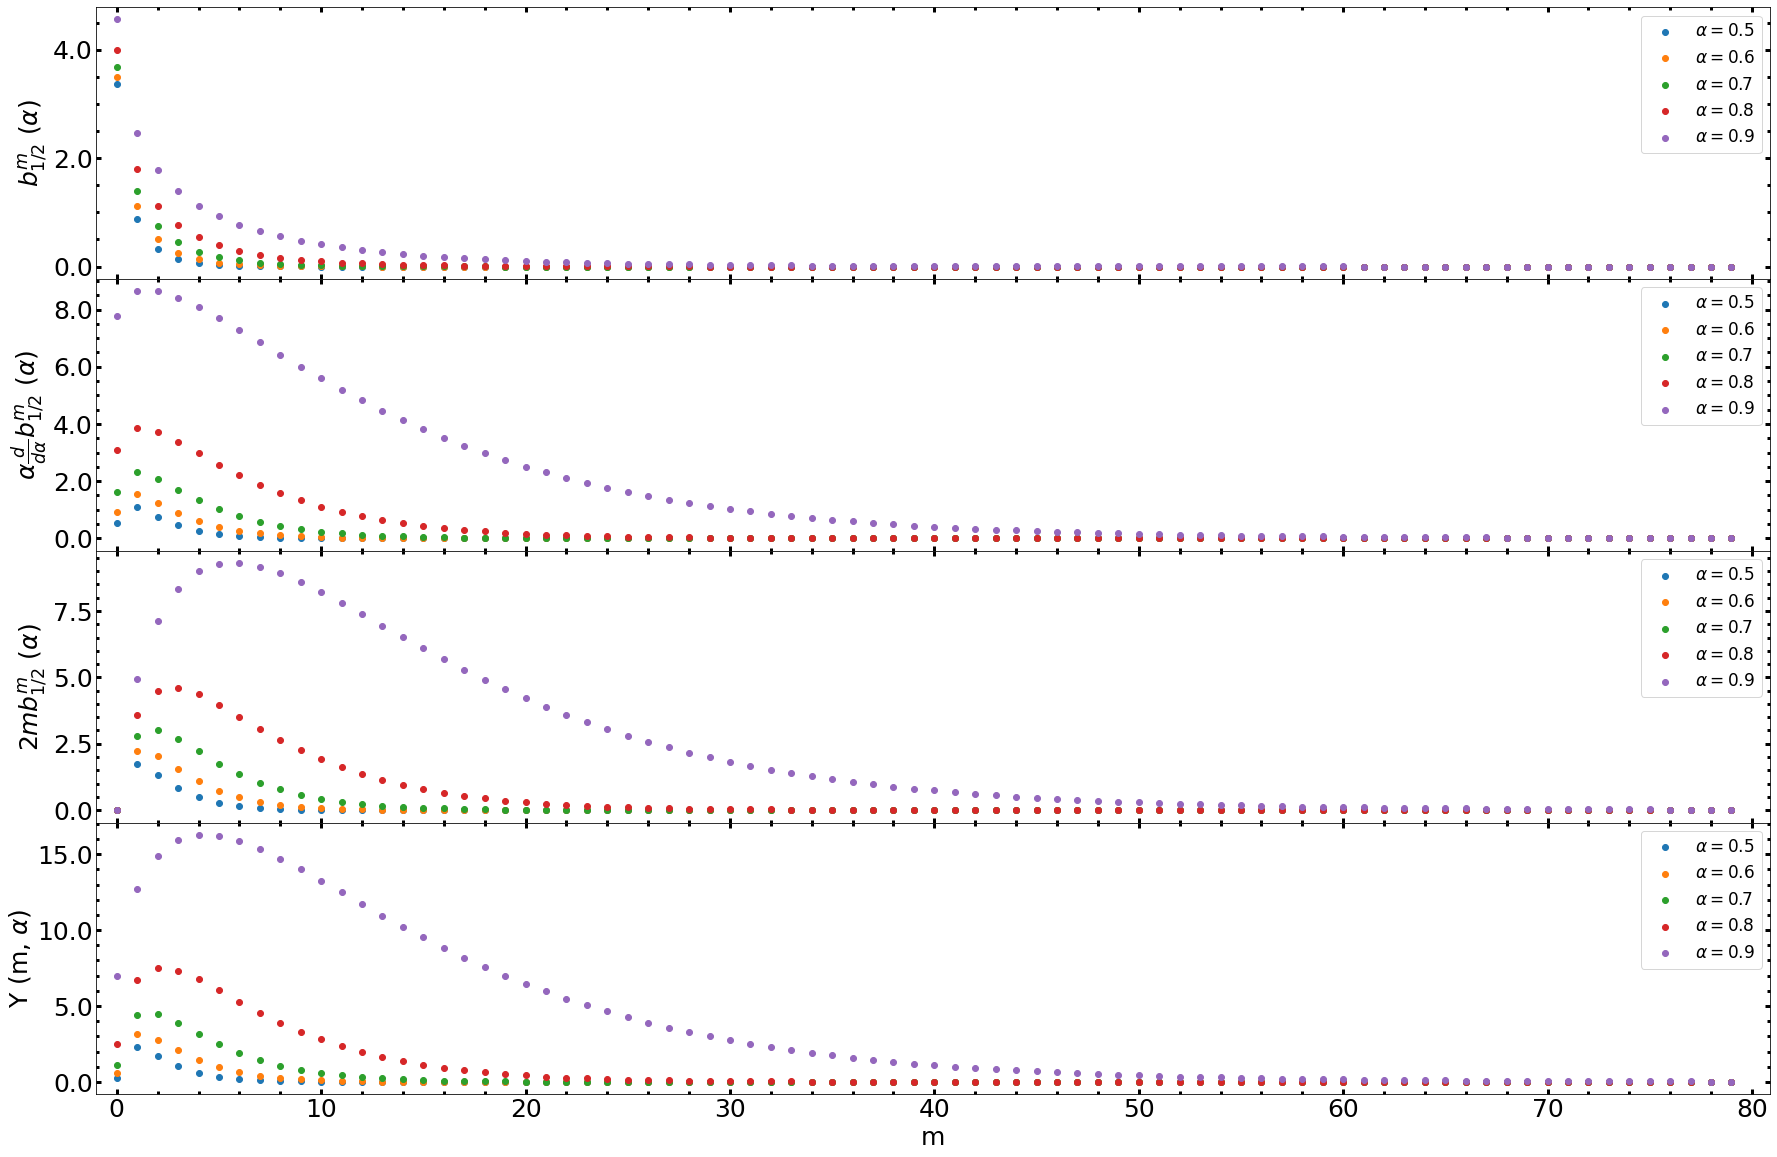
\includegraphics[width=1\linewidth]{laplace_plot_A.png}
    \caption{A numerical plot showing trends for Laplace Coefficient versus $m$, for varying values of $\alpha$.}
    \label{fig:enter-label}
\end{figure}


The trend of behavior of the function $\Upsilon(m,\alpha)$ versus given $\alpha$ values, for varying $m$ values, is characterized by a gradual increase from $\alpha =0.5$, where the values of $\Upsilon(m,\alpha)$  grow as $\alpha$ increases in the interval \([0.5, 1)\). However, a notable shift occurs as the function approaches \(\alpha=1\), signaling the presence of a vertical asymptote around that region. At this point, the function does not simply continue to increase; rather, it starts to increase towards infinity. Mathematically, this behavior is expressed through limits: $\lim_{{\alpha \to 1}} \Upsilon(m,\alpha) = \infty$, implying that the function would exhibit a steep upward slope as $\alpha$ approaches 1, without actually crossing the vertical line $\alpha=1$. The unbounded growth of the function near $\alpha=1$ suggests that the output of the function become arbitrarily large as $\alpha$ gets arbitrarily close to 1, highlighting a characteristic behavior often observed in functions with vertical asymptotes, particularly in cases where the denominator approaches zero as $\alpha$ approaches the location of the asymptote. From figure 13, the limiting case simply shows that for values of $m$ that are fixed and nonzero, 
\begin{equation}
b_{1/2}^{m}(\alpha) \rightarrow \frac{2}{\pi}\left( - \gamma^{*} - \log\left[\frac{1}{2}|m(1-\alpha)|\right] + \mathcal{O}\left(|m(1-\alpha)|^{2}\log|m(1-\alpha)|\right) \right), \quad \forall \alpha \rightarrow 1,
\end{equation}
which shows a clear case of divergence for the Laplace coefficients and its variants, as given on page 245 by \cite{tremaine2023dynamics}. Numerically, the $\gamma^{*}$ is equivalent to $0.577216...$, which is the Euler's constant.


\begin{figure}
    \centering
    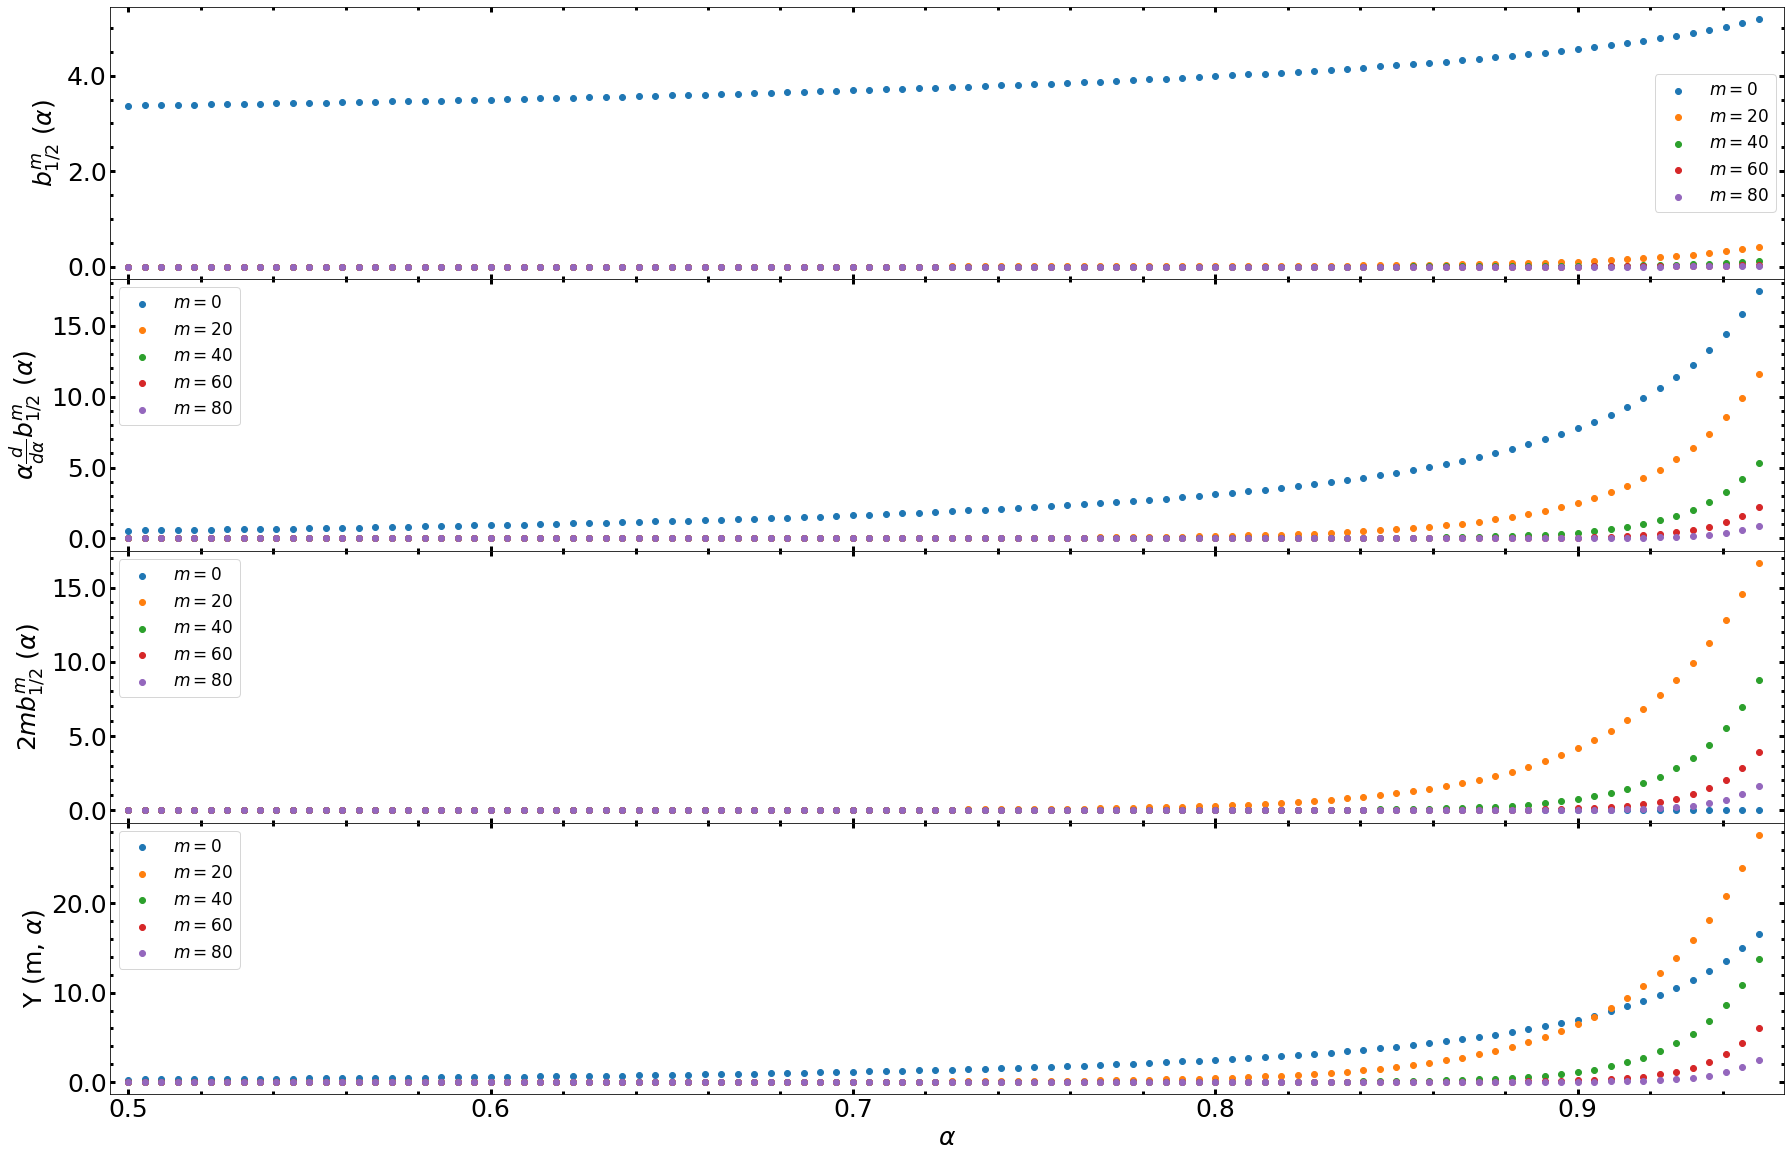
\includegraphics[width=1\linewidth]{laplace_plot_B.png}
    \caption{A numerical plot showing trends for Laplace Coefficient versus $\alpha$, for varying values of $m$.}
    \label{fig:enter-label}
\end{figure}

%.................................%.....................................%......................................

\subsubsection{Sample Wave-fitting Routine and Parameters}

In regard to the wave-fitting routine, we recall our model for the wave-fitting routine, 
\begin{equation}
    y(x) = a(\frac{x-x_{r}}{x_{f}})e^{-\left(\frac{|x-x_{r}|}{x_{d}x_{f}}\right)^{3}}\cos\left(\phi_{0} - \frac{3\pi}{4} - \frac{{(x-x_{r})^2}}{{x_{f}^{2}}}\right)\zeta(\frac{x-x_{r}}{x_{f}}), 
\end{equation}
which when implemented, the aforesaid operation simply produces $a$, $x_{d}$, $\phi_{0}$, $x_{r}$ and $x_{f}$ as the wave-fit parameters.

\vspace{3pt}

\textbf{Note:}

\vspace{3pt}
\textbf{$a$} = Dimensionless amplitude for the density wave-fit.

\vspace{3pt}
\textbf{$x_{d}$} = Damping parameter for the specific density wave.

\vspace{3pt}
\textbf{$\phi_{0}$} = Initial phase value from the wave-fit routine (in radian).

\vspace{3pt}
\textbf{$x_{r}$} = Wave-fit for the resonant radius of the wave (in Kilometer).

\vspace{3pt}
\textbf{$x_{f}$} = Winding parameter (in Kilometer).

\vspace{10pt}
The attached figure illustrates the juxtaposition of two plots: one for the actual dataset from Cassini VIMS (indicated by the blue legend), and the other for the linear density wave-fitting model mentioned earlier (designated by the black legend). The vertical axis corresponds to the normalized optical depth for the section of the ring where the spiral density wave was detected by Cassini VIMS, while the horizontal axis represents the radial offset in relation to the planet's center.
The necessary dimensionless parameters, including amplitude, damping, and winding, are extracted. Initially, we calculate the surface mass density using the winding parameter and subsequently derive the required viscosity. Finally, we convert the dimensionless amplitude of the spiral density wave into the necessary amplitude for the normal-mode oscillation within Saturn's interior that induced such a wave in that specific segment of Saturn's C-ring.
The errors in these measurements for all wave signals are estimated through the conventional bootstrapping technique, which we will describe in the following section.


\begin{figure}[h]
\centering 
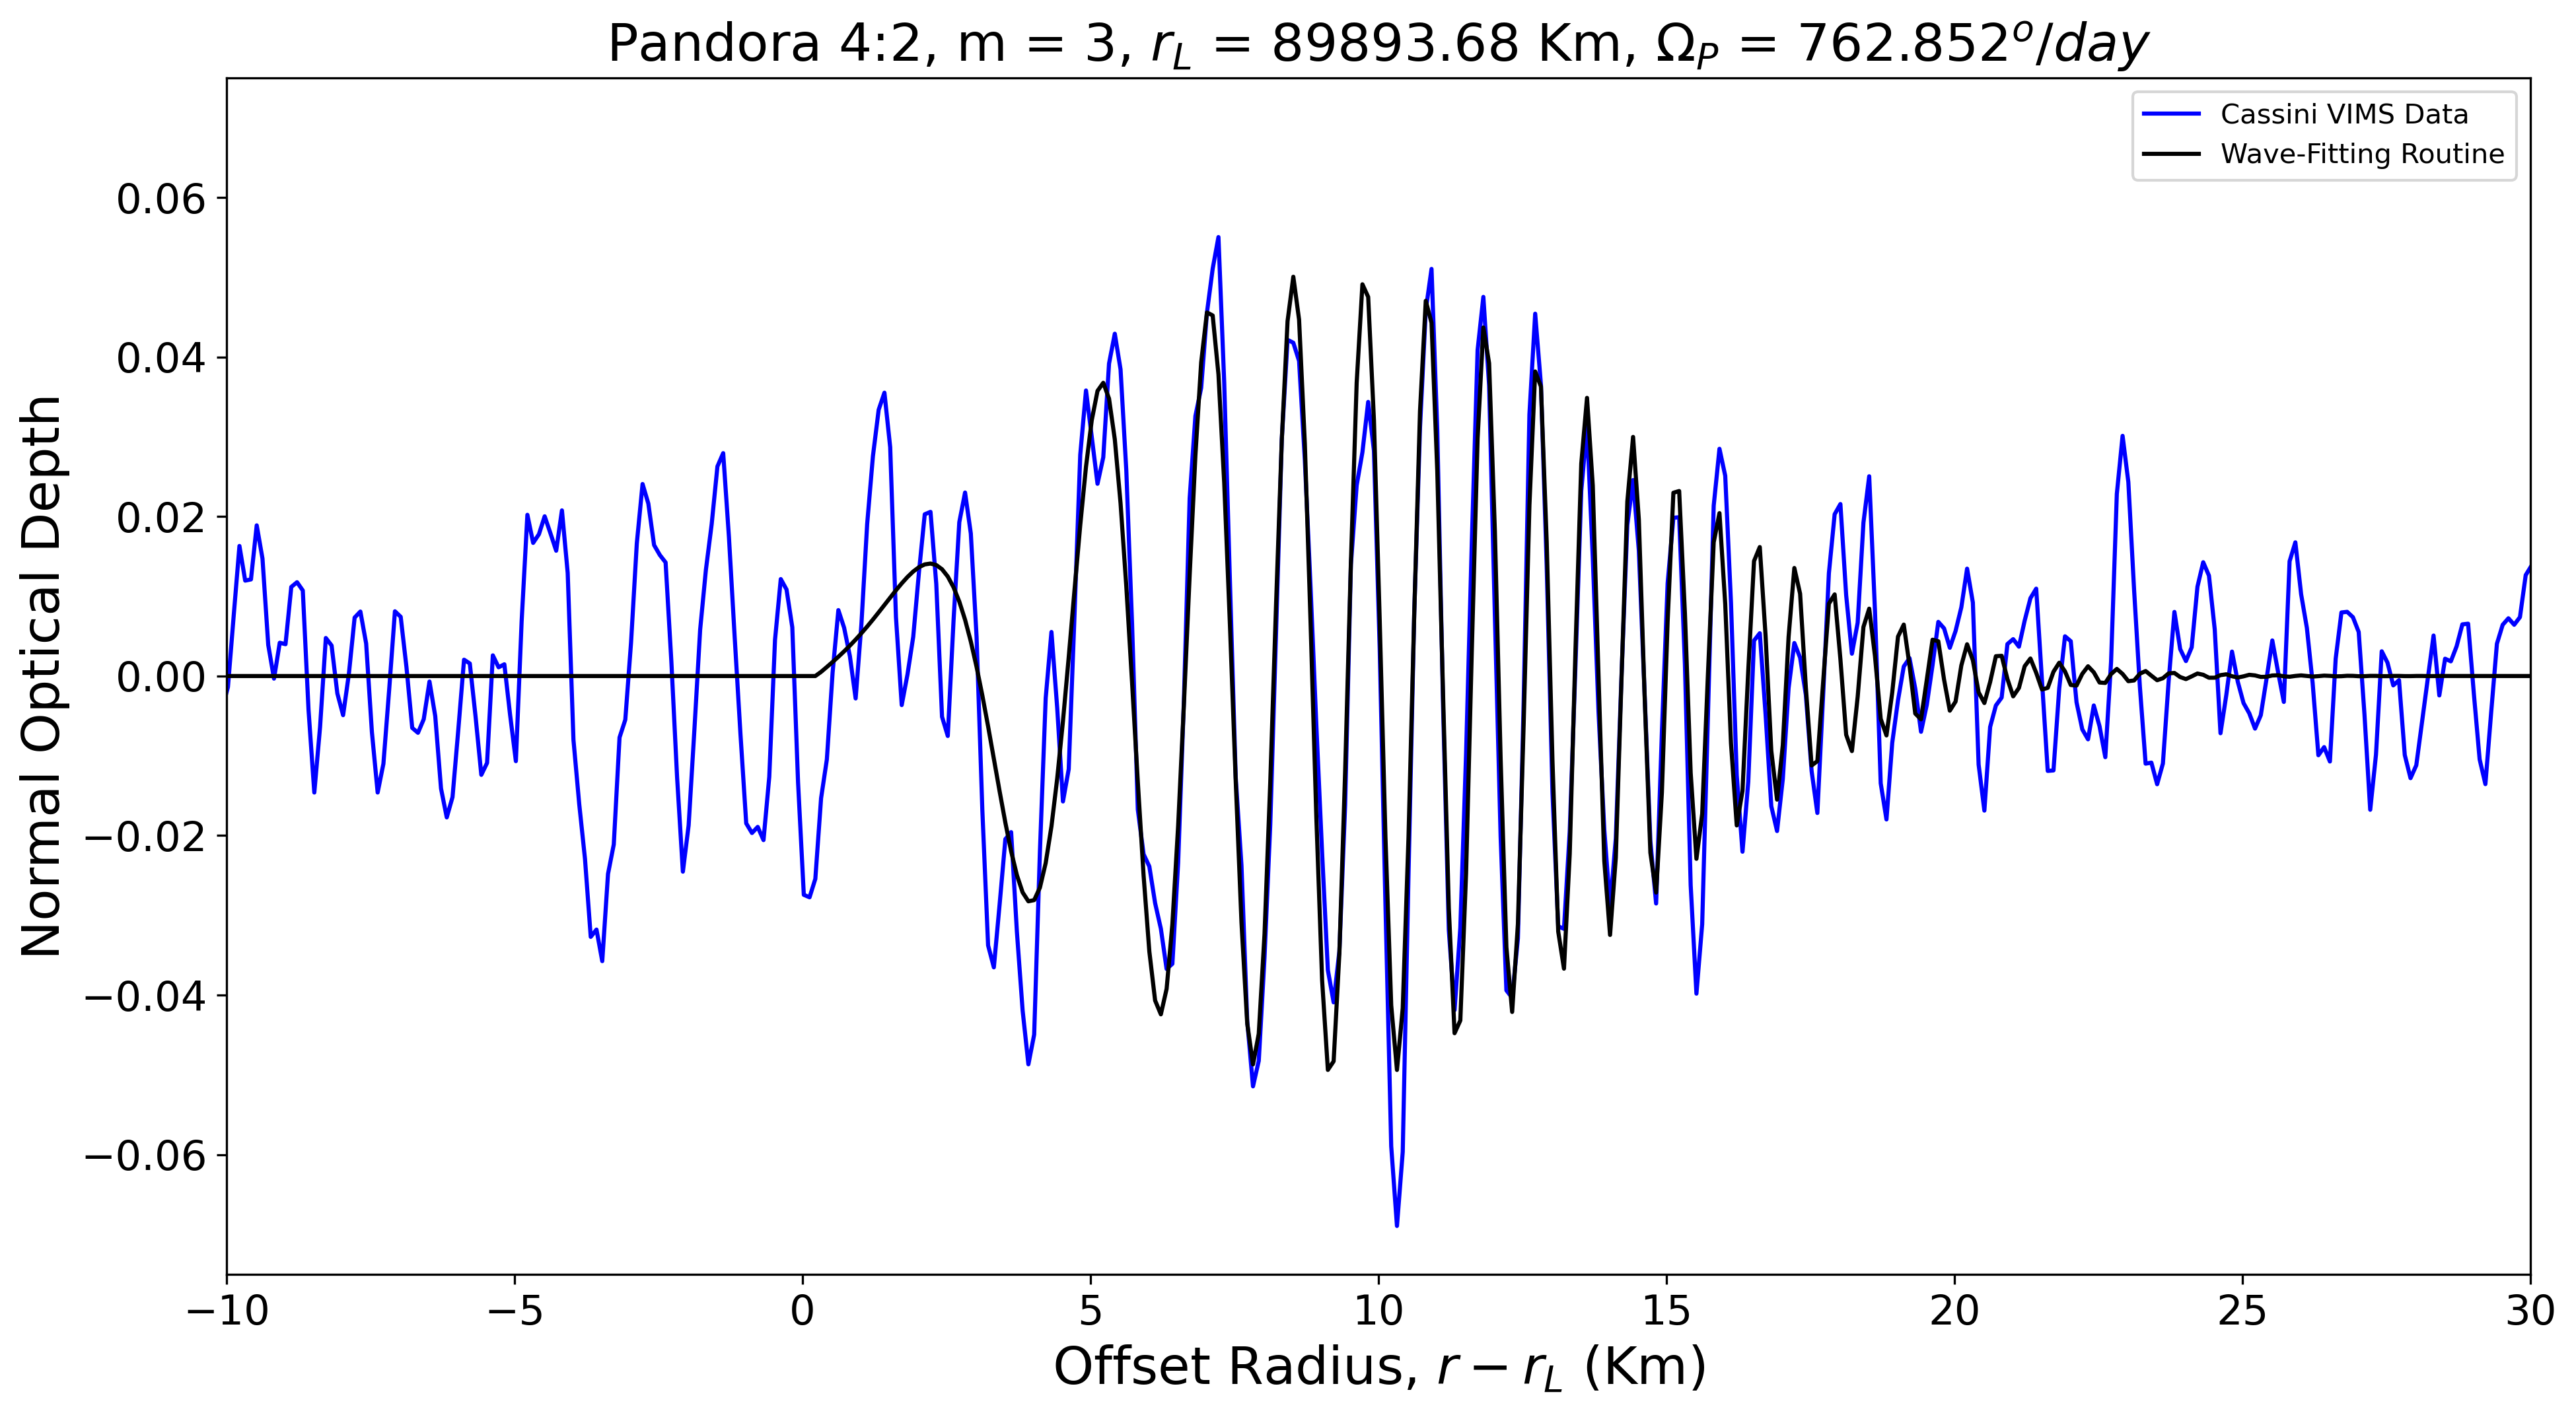
\includegraphics[width=0.7\textwidth]{pandora42.png} 
\caption{A wave-fitting routine for the Pandora 4:2 Satellite resonance.} \label{fig:my_label}
\end{figure}

\begin{table}
\centering
\begin{tabular}{|c|c|c|}
\hline
\textbf{Nomenclature} & \textbf{Symbol} & \textbf{Value} \\
\hline
Resonance label & $m$ & 3 \\
\hline
Resonance location & $r_{L}$ & 89893.68 Km \\
\hline
Pattern speed & $\Omega_{p}$ & 762.852 $^{o}/day$ \\
\hline
Amplitude & a & 0.1829 \\
\hline
Damping Length & $x_{d}$ & 3.9257 \\
\hline
Initial Phase & $\phi_{0}$ & 1.2049 rad \\
\hline
Resonance Offset & $x_{r}$ & 0.3505 Km \\
\hline
Winding Parameter & $x_{f}$ & 2.0115 Km \\
\hline
\end{tabular}
\caption{Parameter values for wave-fitting routine for W84.64}
\end{table}



%are extracted from the routine, as  ( $a$, $x_{d}$, $x_{f}$ and $\sigma_{0}$). These parameters are then used in the required expressions above, to generate the given plots in the next section. 

%......................................................................................
\subsubsection{Robust Data Processing Strategies for Addressing Outliers in Optical Depth Profiles of Saturn's Spiral Density Waves}
In the process of conducting wave-fitting procedures for background optical depth profiles associated with specified spiral density waves excited by Saturn, we encountered data glitches or outliers within the dataset. To address these anomalies during the data preprocessing phase, we followed a systematic approach tailored to the nature of the data and the specific requirements of the linear density wave model. Initially, we identified and confirmed outliers by pinpointing radial regions with significantly elevated data points compared to the rest of the optical depth profiles. Subsequently, we delved into understanding the context of these outliers, consulting domain experts to discern whether they were genuine data points or indicative of errors or anomalies. Visualization techniques, such as box plots or scatter plots, were employed to grasp the distribution of values across different regions of the optical depth profiles, offering a visual representation of outliers. Imputation procedures were then implemented, involving the replacement of anomalous values with calculated estimates. Simple imputation methods, such as using the mean, were applied to mitigate the impact of extreme values and enhance the symmetry of the distribution. It is crucial to exercise caution when considering the removal of outliers, as this decision can significantly influence the analysis, requiring a solid understanding of the data. Finally, data validation and cleaning were carried out, incorporating comparable plots to ensure the consistency of the repaired dataset with expectations. Collaboration with domain experts played a vital role in making informed decisions about handling inconsistent datasets for each optical depth profile. This comprehensive approach ensured the accuracy and reliability of the wave-fitting procedures in the face of data anomalies. The planetary density wave signals adversely affected by the anomalies were \textbf{W74.51} and \textbf{W76.46} respectively. 
%......................................................................................
\subsubsection{Error Analysis for Independent Parameters: Bootstrap Resampling}

Since each density wave profile comprises a series of occultations, there is a requirement for a precise yet efficient method to quantify uncertainties or variations in the (independent) parameters resulting from the wave-fitting routine for each wave signal. Therefore, there is a necessity for bootstrap resampling.

Bootstrap resampling is a powerful statistical technique that involves drawing multiple samples, in this case without replacement, from the observed data to simulate a distribution of parameter values or estimate the uncertainty or variability in a parameter without relying on assumptions about the underlying population distribution\cite{Chernick2007BootstrapMA,davison_hinkley_1997}. By repetitively resampling the data, we can generate a range of potential parameter sets, allowing us to assess the robustness and reliability of the fitted wave profiles. That way we tend to capture the inherent variability in the data and provide a more comprehensive understanding of the uncertainties associated with the density wave parameters\cite{Efron1994AnIT,article}. This method is particularly useful for error analysis in measurements. The following steps outline the process along with relevant equations.

\paragraph{Generate Resampled Datasets:}
Let $\mathbf{X} = \{x_1, x_2, \ldots, x_n\}$ represent the original occultation dataset, from which we can derive measurements of particular wave-fit parameters (for example, the amplitude of a particular wave signal). To perform bootstrap resampling, we generate a class of consistent number of resampled datasets by excluding a portion of the profiles in a given order, denoted as $\mathbf{X}^{*}_B$, and subsequently replacing the previous portion of profiles with a differently ordered set\cite{Chernick2007BootstrapMA,davison_hinkley_1997,Efron1994AnIT,article}. To complete the process, we can set the number of occultation profiles required for the bootstrap procedure as,
\begin{equation}
    \mathcal{X}_{b}= \mathbf{X}-\mathbf{X}^{*}_B.
\end{equation}

\paragraph{Compute the Parameter of Interest:}
For each resampled dataset $\mathcal{X}_{b}$, we calculate the parameter of interest, denoted as $\theta$. For example, if the interest is in the mean, the parameter estimate for the $b$th resampled dataset, denoted as $\theta^{*}_{b}$, is calculated as\cite{Chernick2007BootstrapMA,davison_hinkley_1997,Efron1994AnIT,article}:
\begin{equation}
\theta^{*}_{b} = g(\mathcal{X}_{b}),
\end{equation}
where $g(.)$ represents the function or statistic used to calculate the parameter estimate.
\paragraph{Calculate Variability:}
After obtaining the parameter estimates $\theta^{*}_{b}$ for all resampled datasets, we analyze the distribution of these estimates to determine variability. Calculate the mean estimate ($\bar{\theta}^{*}$) and standard deviation estimate ($s^{*}$) as follows\cite{Chernick2007BootstrapMA,davison_hinkley_1997,Efron1994AnIT}:
\begin{equation}
\bar{\theta}^{*} = \frac{1}{N_{b}}\sum_{b=1}^{N_{b}}\theta^{*}_{b},
\end{equation}

\begin{equation}
s^{*} = \sqrt{\frac{1}{N_{b}-1}\sum_{b=1}^{N_{b}}(\theta^{*}_{b} - \bar{\theta}^{*})^2}
\end{equation}

For our case, we can assume the estimate of the Standard Error ($SE$) to be equivalent to the aforesaid standard deviation estimate ($s^{*}$) for the sample dataset in the previous step, and apply the aforesaid results to our work. Note that in the provided equation, we are calculating the sample standard deviation estimate ($s^{*}$), which typically involves using the divisor $N_{b}-1$ instead of $N_{b}$ when calculating the variance to account for the fact that we are working with a sample or portion of the dataset rather than the entire population of the dataset.

Based on the distribution of the parameter estimates, we can express the uncertainty in the measurement. Bootstrap resampling allows for estimating the sampling variability of a parameter without assuming a specific distribution, providing a robust method for error analysis in measurements. In essence, bootstrap resampling serves as a powerful tool for refining our analyses and ensuring that the derived parameters are not overly sensitive to specific data points, contributing to a more robust and reliable characterization of density wave profiles.

%......................................................................................
\subsubsection{Error Analysis for Dependent Parameters: Method of Propagation}
In scientific and engineering applications, it is common to encounter functions of multiple variables where each variable has associated uncertainties. Understanding how uncertainties propagate through these functions is crucial for assessing the reliability of results. In this section, we explore the error propagation formula, beginning with the general case where variables may be correlated. We leverage the Taylor series expansion and properties of covariance matrices to derive a comprehensive expression for the uncertainty in a function. Additionally, we simplify this expression in the special case where variables are uncorrelated, providing a more practical and computationally efficient formula.

%We start by invoking the Taylor series expansion to express a function \( f(\mathbf{x}) \) as a sum of partial derivatives around a specific point \( \mathbf{x}_0 \). This allows us to derive the differential of \( f \) and subsequently formulate the error propagation formula. In the general case, we account for correlations between variables through the covariance matrix.

%When variables are uncorrelated, the error propagation formula simplifies, making the computation more straightforward. We explore this special case, providing a simplified expression that is often used in practice.

Deriving the error propagation formula from Taylor's theorem for a general case with \( n \) variables \( x_1, x_2, \ldots, x_n \) and a function \( w = f(x_1, x_2, \ldots, x_n) \), Taylor's theorem for a multivariable function is given by\cite{taylor2022introduction,LUO201723}:
\begin{equation}
f(x_1 + \Delta x_1, x_2 + \Delta x_2, \ldots, x_n + \Delta x_n) \approx f(x_1, x_2, \ldots, x_n) + \sum_{i=1}^{n} \frac{\partial f}{\partial x_i} \Delta x_i
\end{equation}

Now, consider the function \( w = f(x_1, x_2, \ldots, x_n) \) and introduce uncertainties:
\begin{equation}
w(x_1 + \Delta x_1, x_2 + \Delta x_2, \ldots, x_n + \Delta x_n) \approx w(x_1, x_2, \ldots, x_n) + \sum_{i=1}^{n} \frac{\partial w}{\partial x_i} \Delta x_i
\end{equation}

Now, square both sides:
\begin{equation}
(w + \Delta w)^2 \approx w^2 + 2w\Delta w + (\Delta w)^2
\end{equation}

Taking the expectation and neglecting higher-order terms:
\begin{equation}
\langle (\Delta w)^2 \rangle \approx \sum_{i=1}^{n} \langle \left(\frac{\partial w}{\partial x_i}\right)^2 \rangle \langle (\Delta x_i)^2 \rangle + 2 \sum_{i=1}^{n} \sum_{j=i+1}^{n} \langle \frac{\partial w}{\partial x_i} \frac{\partial w}{\partial x_j} \rangle \langle \Delta x_i \Delta x_j \rangle
\end{equation}

Here, \( \langle \cdot \rangle \) denotes the expectation value.

The covariance terms (\( \text{Cov}(x_i, x_j) \)) are introduced in the correlation terms:
\begin{equation}
\langle \Delta x_i \Delta x_j \rangle = \text{Cov}(x_i, x_j)
\end{equation}

Now, we can rewrite the expression:
\begin{equation}
\langle (\Delta w)^2 \rangle \approx \sum_{i=1}^{n} \langle \left(\frac{\partial w}{\partial x_i}\right)^2 \rangle \langle (\Delta x_i)^2 \rangle + 2 \sum_{i=1}^{n} \sum_{j=i+1}^{n} \langle \frac{\partial w}{\partial x_i} \frac{\partial w}{\partial x_j} \rangle \text{Cov}(x_i, x_j)
\end{equation}

Finally, dividing both sides by \(w^2\) and taking the square root, we get the error propagation formula with correlation for \( n \) variables\cite{articleb,taylor2022introduction,weisstein2000error,LUO201723}:
\begin{equation}
\frac{\sigma_w}{w} \approx \sqrt{\sum_{i=1}^{n} \left(\frac{\partial w}{\partial x_i}\right)^2 \left(\frac{\sigma_{x_i}}{x_i}\right)^2 + 2 \sum_{i=1}^{n} \sum_{j=i+1}^{n} \frac{\partial w}{\partial x_i} \frac{\partial w}{\partial x_j} \frac{\text{Cov}(x_i, x_j)}{x_i x_j}}
\end{equation}

This formula accounts for both the individual uncertainties in each variable (\( \frac{\sigma_{x_i}}{x_i} \)) and the correlations between different pairs of variables (\( \text{Cov}(x_i, x_j) \)). For the case of non-correlation, where all covariance terms are zero (\( \text{Cov}(x_i, x_j) = 0 \) for all \( i \neq j \)), the formula simplifies to the standard error propagation formula:

\begin{equation}
\frac{\sigma_w}{w} \approx \sqrt{\sum_{i=1}^{n} \left(\frac{\partial w}{\partial x_i}\right)^2 \left(\frac{\sigma_{x_i}}{x_i}\right)^2}
\end{equation}

Examining the spread of errors through differential calculus proves effective for models defined by smooth and differentiable relationships. This method offers valuable insights into error propagation and uncertainty, particularly in compact theoretical models. It establishes a conceptual framework for understanding how variability moves through complex systems of equations\cite{articleb}. However, limitations exist. The approach assumes differentiability, making it unsuitable for models with discontinuities, step functions, or conditional logic. Additionally, it is inherently local, disregarding higher-order terms and lacking information on outliers\cite{articleb}. Variance-based error analysis assumes a symmetric distribution, limiting its applicability to skewed distributions like the log-normal distribution\cite{MCKAY199944}. Despite these drawbacks, the differential analysis remains a valuable guide for comprehending uncertainty propagation in predictive models\cite{articleb,taylor2022introduction,LUO201723}.
%......................................................................................

\subsubsection{Discussions on Model Parameters For the Wave-Fit Procedures:}

Actually, there is no one-size-fits-all reason for why we chose to include the fitting parameters described above in our theoretical model. It was an essential power-play to enable us to strike a balance between the complexity of the theoretical model and the need to accurately capture the underlying behavior of the data. Our decision was guided by a combination of several factors with their succinct descriptions below.

1. \textbf{Generalization:} The goal of modeling is often to make predictions or inferences on new, unseen data. Models with too many parameters may fit the training data extremely well but fail to generalize to new data. Reducing the number of parameters can lead to models that generalize better \cite{james2013introduction}.

2. \textbf{Quality of Data:} High-quality, precise data can often support more complex models with more parameters. Since our data has some traces of noise, using a simpler model with fewer parameters might be more appropriate to avoid overfitting \cite{bishop2006pattern}.

3. \textbf{Overfitting:} Overfitting is a common concern when fitting non-linear models with a large number of parameters to non-linear data. Overfitting occurs when the model captures noise and fluctuations in the data rather than the underlying trend or pattern. Reducing the number of parameters helps prevent overfitting by making the model less complex and more robust to noise \cite{bishop2006pattern}.

4. \textbf{Interpretability:} Non-linear models with a high number of parameters can be challenging to interpret. By reducing the number of parameters, we can make the model more interpretable, as it becomes easier to understand the functional relationships between input variables and the model's predictions \cite{molnar2020interpretable}.

5. \textbf{Computational Efficiency:} Fitting non-linear models with a large number of parameters can be computationally intensive and time-consuming. Reducing the parameter space makes the optimization problem more tractable and faster to converge using tools like SciPy \cite{nocedal2006numerical}.

6. \textbf{Stability:} Non-linear regression can be sensitive to the initial parameter values, and models with a high number of parameters may have multiple local minima in the objective function (like degeneracies in the wave-fit parameters). Reducing the number of parameters can make the optimization process more stable and less prone to getting stuck in local optima \cite{nocedal2006numerical}.

7. \textbf{Bias-Variance Trade-off:} Non-linear models with many parameters are prone to having high variance, which can lead to unpredictable and erratic behavior. Reducing the number of parameters can reduce model variance and improve its reliability \cite{hastie2009elements}.

8. \textbf{Data Requirements:} Fitting complex non-linear models with numerous parameters often requires a substantial amount of data to estimate those parameters accurately. Since we are working with aliquot amount of Cassini VIMS dataset, reducing the number of parameters can help prevent overfitting and lead to more stable and trustworthy estimates.

9. \textbf{Occam's Razor:} Ceteris paribus, this principle suggests that simpler explanations (or models) should be preferred to their complex versions. In many cases, a simpler model with fewer parameters is preferred, provided it can adequately describe the trend of dataset involved. It is easier to interpret and generalize a simple model, as opposed to a complex model \cite{Sober2015-SOBORA}.





\subsection{Preliminary Result I: Satellite Resonances}
In this section, we feature the predicted gravitational potential estimate results for satellite spiral density waves, as well as the computed estimates of gravitational potentials gotten through the aforementioned techniques. 

\subsubsection{Satellite Waves: Predicted Estimates for Gravitational Potential}
Starting with the satellite wave, we present the given table containing predicted values for the respective gravitational potentials, using the normalized torque expression for equation (61) from \cite{Hedman_2022}:
\begin{equation}
    \Psi_{m,p}^{'} = \sqrt{\frac{3|m - 1|n_{L}^{2}}{m\pi^{2}} \left|\frac{\mathcal{T}}{\sigma_{0}}\right|},
\end{equation}
where $n_{L}^{2} = \frac{G M_{P}}{r_{L}^{3}}$.


\begin{table}
\centering
\rotatebox{0}{
\begin{tabular}{|c|c|c|c|c|}
\hline
Resonance Name & $m$ & $r_{L}$ (Km) & $\mathcal{T}/\sigma_{0}$ (Km$^{4}$s$^{-2}$) & $\Psi_{m,p}^{'} (m^{2}s^{-2})$ \\
\hline
Mimas 4:1 & 2 & 74890.067 & -8.987453e-08 & 0.035125 \\
Pan 2:1 & 2 & 85105.021 & -2.971890e-09 & 0.005273 \\
Atlas 2:1 & 2 & 87645.684 & -5.346249e-09 & 0.006767 \\
Prometheus 4:2 & 3 & 88434.120 & -2.651270e-10 & 0.001717 \\
Mimas 6:2 & 3 & 89883.135 & -9.726598e-10 & 0.003209 \\
Pandora 4:2 & 3 & 89893.680 & -7.171256e-10 & 0.002755 \\
\hline
\end{tabular}
}
\caption{Predicted data for spiral density waves excited by Saturn's Satellite resonances.}
\end{table}

\subsubsection{Satellite Waves: Parameters from Wave-fitting Routine}
A wave-fitting routine was applied to data collected on satellite waves within Saturn's rings, revealing information about their properties and behavior. The analysis focused on spiral density waves, which are prominent features within the rings and are excited by gravitational resonances with Saturn's moons. The table of values and plots from the wave-fitting routine for satellite resonances generated by Saturn's moons, are displayed below. The details provided in the table are summarized below.

\textbf{Radial Range} Specifies the range of radial distances affected by each resonance. \textbf{$m$} indicates the number of spiral arms generated by the resonance. \textbf{Resonance Location} specifies the precise radial location of the density wave signal. The \textbf{Pattern Speed} indicates the speed associated with the resonance in degrees per day. The \textbf{$a_{fit}$} represents the amplitude of the density wave generated for the fit routine. This is influenced by the mass of the perturber (say, a moon or planet). It provides information about the strength of the density wave. The damping parameter \textbf{$x_{d}$} measures the rate at which the wave's amplitude decreases over distance. Higher values indicate faster decay. The initial phase \textbf{$\phi_{0}$} represents the phase of the wave in radians, at resonance. Resonance Offset \textbf{$x_{r}$} denotes the precision in resonance location provided by the model for the given wave generated by Saturn's moon. It specifies the offset of the resonance from a reference point. Winding Parameter \textbf{$x_{f}$} controls the number of cycles of the wave-fit model and sometimes the rate at which the wave-fit grows or decays.

Overall, these parameters provide detailed information about the characteristics and behavior of the density waves excited by Saturn's satellite resonances. They are essential for understanding the dynamics of Saturn's rings and the interactions between the planet and its ring(s).

Analysis of such waves reveals key characteristics and resonance patterns. It identified distinct wave patterns associated with resonances involving Mimas, Pan, Atlas, Prometheus, and Pandora. These resonances occur at specific radial distances within the rings, where the orbital periods of ring particles and moons align in integer ratios. The amplitudes of the spiral density waves, represented by the parameter $a_{fit}$, varied across different resonances. Mimas 4:1 and Atlas 2:1 resonances exhibited relatively higher amplitudes compared to other resonances. The damping parameters and radial offsets also varied among resonances. The Pan 2:1 resonance displayed a notably longer wavelength compared to other resonances.

%...........................................................................

\begin{table}
\centering
\vspace{-1.5cm}
\rotatebox{90}{
\begin{tabular}{|c|c|c|c|c|c|c|c|c|c|c|}
\hline
\stackon[0pt]{\textbf{Name}}{\stackon[3pt]{\textbf{Resonance}}{}} & \stackon[0pt]{\stackon[3pt]{\textbf{Range (Km)}}{\textbf{Radial}}} & \stackon[0pt]{\stackon[3pt]{\textbf{Location (Km)}}{\textbf{Resonance}}} & $l$ & \textbf{$m$} & \stackon[0pt]{\stackon[3pt]{\textbf{Speed ($^{o}$/day)}}{\textbf{Pattern}}} & \textbf{$a_{fit}$ (Units)} & \textbf{$x_{d}$ (Units)} & \textbf{$\phi_{0}$ (rad)} & \textbf{$x_{r}$ (Km)} & \textbf{$x_{f}$ (Km)} \\
\hline
Mimas 4:1 & 74880.00 - 74895.00 & 74890.07 & - & 2 & 762.988 & 0.2229 $\pm$ 0.0305 & 2.7986 $\pm$ 0.0723 & -4.1869 $\pm$ 0.8471 & 2.6125 $\pm$ 1.0523 & 1.5657 $\pm$ 0.2979 \\

Pan 2:1 & 85090.00 - 85130.00 & 85105.02 & - & 2 & 626.032 & 0.0139 $\pm$ 0.0013 & 4.5691 $\pm$ 0.1661 & -6.2832 $\pm$ 2.7684e-12 & 1.1439 $\pm$ 0.0288 & 2.6895 $\pm$ 0.0088 \\

Atlas 2:1 & 87640.00 - 87650.00 & 87645.68 & - & 2 & 598.312 & 0.1684 $\pm$ 0.0200 & 2.2372 $\pm$ 0.0908 &   -0.8166 $\pm$ 0.1451 & 0.3621 $\pm$ 0.0346 & 1.0447 $\pm$ 0.0149 \\

Prometheus 4:2 & 88420.00 - 88440.00 & 88434.12 & - & 3 & 782.128 & 0.0067 $\pm$ 0.0003 & 5.8369 $\pm$ 0.0941 & 0.2629 $\pm$ 0.1654 & 0.4764 $\pm$ 0.0652 & 1.6954 $\pm$ 0.0068 \\

Mimas 6:2 & 89870.00 - 89890.00 & 89884.00 & - &  3 & 762.977 & 0.0128 $\pm$ 0.0013 & 4.8527 $\pm$ 0.2113 &    -1.7461 $\pm$ 0.8968 & 1.2660 $\pm$ 0.4235 & 1.6616 $\pm$ 0.0572 \\

Pandora 4:2 & 89887.00 - 89897.00 & 89893.68 & - & 3 & 762.852 & 0.0074 $\pm$ 0.0003 & 6.9140 $\pm$ 0.0368 &   -3.2364 $\pm$ 0.0662 & 0.2341 $\pm$ 0.0271 & 1.8745 $\pm$ 0.0025 \\

\hline
\end{tabular}
\vspace{-1.0cm}
}
\caption{Data for wave-fitting parameters for spiral density waves excited by Saturn's Satellite resonances.}
\end{table}

%................................................................

\subsubsection{Model Computations for Ring Properties using Satellite Resonances}

The mass extinction coefficient ($\kappa$) plays a crucial role in understanding the properties and composition of Saturn's rings. It relates the average optical depth ($\tau_{av}$), which measures how much light the ring system blocks, to the surface mass density ($\sigma_{0}$), which indicates the amount of mass per unit area within the ring. It simply tells us how efficiently the ring particles block light based on their mass. The mass extinction coefficient is significant, since it reveals ring particle properties such as the following below:

\textbf{Size:} A higher $\kappa$ value generally implies smaller particles. This is because smaller particles have a larger surface area for their mass, leading to more efficient light blocking ability for that section of Saturn's C-ring. Variations in $\kappa$ across different regions of the rings could infer the size distribution of particles in those regions.

\textbf{Composition:} Different materials have different opacities (that is, how well they block light). Analyzing variations in $\kappa$ alongside spectral data can help identify the composition of ring particles, such as whether they are mostly ice, rock, or a mixture.

The mass extinction coefficient $\kappa$ is very crucial in ring dynamics for interpreting the observed brightness variations within the rings of Saturn, often caused by density waves. Trends in surface mass density and mass extinction coefficient could help model how light interacts with particles in the rings, and can buttress our understanding of the distribution and dynamics of density waves across the rings, revealing insights into the gravitational interactions between ring particles, Saturn and Saturn's moons. Collisions between ring particles can break them down, altering their size and composition. Measuring $\kappa$ over time can also help track these changes and understand the evolution of the ring system.

Building upon the initial data presentation for satellite resonances, this section highlights the implications of the model computations for the aforesaid parameters.

\textbf{Mimas 4:1 Resonance:}
This resonance occurs between Saturn's moon Mimas and its C-ring. The average optical depth ($\tau_{av}$) is 0.034336, indicating relatively low opacity, while surface mass density ($\sigma_{0}$) is $1.057663 g/cm^{2}$. The mass extinction coefficient ($\kappa$) is 0.032464 $cm^{2}/g$. Overall, this resonance suggests a relatively moderate light blocking efficiency and low mass density within the C-ring around Mimas.

\textbf{Pan 2:1 Resonance:}
This resonance involves Saturn's moon Pan and its C-ring. $\tau_{av}$ is 0.082371, indicating higher opacity compared to the Mimas resonance. $\sigma_{0}$ is $1.871221 g/cm^{2}$, suggesting a denser region of the C-ring around Pan. $\kappa$ is 0.044020 $cm^{2}/g$, indicating a more efficient light-blocking capability per unit mass compared to the Mimas resonance. Since the Pan 2:1 resonance presents the highest $\sigma_{0}$ value in the table, this might indicate a significantly denser concentration of ring particles in this region, during satellite resonances. The higher $\kappa$ value might also suggest that particles here are more efficient at absorbing or scattering light.

\textbf{Atlas 2:1 Resonance:}
This resonance occurs between Saturn's moon Atlas and its C-ring. Here, $\tau_{av}$ is 0.061705, indicating moderate opacity. $\sigma_{0}$ is around $0.249596 g/cm^{2}$, suggesting a lower mass density compared to the other resonances. $\kappa$ is 0.247220 $cm^{2}/g$, indicating a relatively high light-blocking efficiency per unit mass, despite the lower mass density. Intriguingly, the Atlas 2:1 resonance shows the lowest $\sigma_{0}$ value among the listed resonances. This might suggest a much sparser particle distribution compared to other regions of the C-ring, during satellite resonances. The low $\kappa$ value further supports this notion, implying a lower overall amount of material present to interact with light. This finding might raise potential questions about the mechanisms causing such depleted density within this region of the C-ring, during the specified satellite resonance phenomenon.

\textbf{Prometheus 4:2 Resonance:}
This resonance involves Saturn's moon Prometheus and its C-ring, with $\tau_{av}$ around 0.241621, indicating higher opacity. $\sigma_{0}$ is $1.275612 g/cm^{2}$, suggesting a moderate mass density. $\kappa$ is 0.189415 $cm^{2}/g$, indicating a moderate light-blocking efficiency per unit mass. The Prometheus 4:2 resonance exhibits moderate $\sigma_{0}$ and $\kappa$ values, falling within the average range. However, it is important to note the larger uncertainties associated with both $\sigma_{0}$ and $\kappa$ in this case. A similar occurrence for the Mimas resonances is likely at play in this case. Additional observations could provide more insights into the Prometheus and Mimas satellite resonances.

\textbf{Mimas 6:2 Resonance:}
This resonance occurs between Saturn's moon Mimas and its C-ring. $\tau_{av}$ is roughly 0.340543, indicating relatively high opacity, while $\sigma_{0}$ is around $1.148003 g/cm^{2}$, suggesting a moderate mass density. And $\kappa$ is 0.296640 $cm^{2}/g$, indicating a relatively high light-blocking efficiency per unit mass. Similar to the 4:1 resonance, the Mimas 6:2 resonance shows moderate $\sigma_{0}$ and $\kappa$ values. Investigating the subtle differences in $\sigma_{0}$ and $\kappa$ between the two Mimas resonances could unveil valuable information about how the number of moons involved in a resonance influences ring particle behavior.

\textbf{Pandora 4:2 Resonance:}
This resonance involves Saturn's moon Pandora and its C-ring. $\tau_{av}$ is 0.361360, indicating the highest opacity among the listed resonances. $\sigma_{0}$ is $1.460548 g/cm^{2}$, suggesting a higher mass density. $\kappa$ is 0.247414 $cm^{2}/g$, indicating a moderate light-blocking efficiency per unit mass. Finally, the Pandora 4:2 resonance presents the highest $\kappa$ value alongside a moderate $\sigma_{0}$. This suggests a relatively dense particle population with high light absorption or scattering efficiency, during such resonance phenomenon.
%.......................................................................................

\begin{table}
\centering
\rotatebox{90}{
%\begin{tabular}{lllll}
\begin{tabular}{|c|c|c|c|c|c|c|c|c|}
\hline

\stackon[0pt]{\textbf{Name}}{\stackon[3pt]{\textbf{Resonance}}{}} & \stackon[0pt]{\stackon[3pt]{\textbf{Range (Km)}}{\textbf{Radial}}} & \stackon[0pt]{\stackon[3pt]{\textbf{Location (Km)}}{\textbf{Resonance}}} & $l$ & \textbf{$m$} & $\tau_{av}$ & $\sigma_{0} (g/cm^{2})$ & $\kappa = \frac{\tau_{av}}{\sigma_{0}} (cm^{2}/g)$  & $\nu (cm^{2}/s)$ \\
\hline

Mimas 4:1 & 74880.00 - 74895.00 & 74890.07 & - & 2 & 0.034336 & 1.057663 $\pm$ 0.402423 & 0.032464 $\pm$ 0.012352 & 9.483924 $\pm$ 5.462388 \\
Pan 2:1 & 85090.00 - 85130.00 & 85105.02 & - & 2 & 0.082371 & 1.871221 $\pm$ 0.012231 & 0.044020 $\pm$ 0.000288 & 8.041822 $\pm$ 0.880359 \\
Atlas 2:1 & 87640.00 - 87650.00 & 87645.68 & - & 2 & 0.061705 & 0.250998 $\pm$ 0.007156 & 0.245840 $\pm$ 0.007009 & 3.732417 $\pm$ 0.481570 \\
Prometheus 4:2 & 88420.00 - 88440.00 & 88434.12 & - & 3 & 0.241621 & 1.275612 $\pm$ 0.010282 & 0.189415 $\pm$ 0.001527 & 1.768575 $\pm$ 0.088186 \\
Mimas 6:2 & 89870.00 - 89890.00 & 89884.00 & - & 3 & 0.340543 & 1.148003 $\pm$ 0.079018 & 0.29664 $\pm$ 0.020418 & 2.781585 $\pm$ 0.463107 \\
Pandora 4:2 & 89887.00 - 89897.00 & 89893.68 & - & 3 & 0.361360 & 1.460548 $\pm$ 0.003932 & 0.247414 $\pm$ 0.000666 & 1.380620 $\pm$ 0.022726 \\

\hline
\end{tabular}
}
\caption{Data for Average Optical Depth ($\tau_{av}$), Surface Mass Density ($\sigma_{0}$), Mass extinction coefficient ($\kappa$) and Viscosity($\nu$) estimates from theoretical model for spiral density waves excited by Saturn's Satellite resonances.}
\end{table}

%.......................................................................................................
%.......................................................................................................

The table also presents the dataset on satellite resonance viscosity ($\nu$) estimates derived from our theoretical model. Here, $\nu (cm^{2}/s)$ represents the viscosity, which indicates the resistance within Saturn's C-ring, offered to the flow or propagation of density waves by the particles making up the resonance location of the specific wave. Higher viscosity implies higher resistance to propagation of the aforesaid density waves.

\textbf{Mimas 4:1:}
This resonance is associated with Mimas, one of Saturn's moons. The damping parameter ($x_d$) suggests a moderate rate of amplitude decay, while the viscosity ($\nu$) indicates relatively high resistance within Saturn's C-ring.

\textbf{Pan 2:1:}
Pan's 2:1 resonance indicates a wider radial range compared to Mimas 4:1. The damping parameter is higher, suggesting a faster decay of density waves. However, the viscosity remains moderately high, indicating significant resistance to flow within the affected region.

\textbf{Atlas 2:1:}
This resonance associated with Atlas exhibits a narrower radial range and a relatively lower damping parameter compared to Pan 2:1. The viscosity is moderate, indicating a moderate resistance to ring particle interactions within the affected region.

\textbf{Prometheus 4:2:}
This resonance, associated with Prometheus, features a wider radial range and a higher number of spiral arms (3). The damping parameter is relatively high, indicating a fast decay of density waves, while the viscosity is lower compared to others, suggesting less resistance to the flow of particle interactions within the affected region.

\textbf{Mimas 6:2:}
This resonance associated with Mimas shows a moderate damping parameter and viscosity. The radial range and the number of spiral arms are similar to Prometheus 4:2, but both damping and viscosity values are slightly lower.

\textbf{Pandora 4:2:}
The resonance associated with Pandora exhibits a wider radial range and a higher damping parameter, indicating a slower decay of density waves compared to other resonances. The viscosity is the lowest among all resonances, suggesting relatively less resistance to the flow of particle interactions within the affected region.

The damping parameters vary across the different resonances, indicating varying rates of decay in the amplitude of the density waves. For instance, Prometheus 4:2 has a relatively high damping parameter (5.8369), suggesting a faster decay compared to others like Mimas 4:1 (2.7986). The viscosity also varies, implying differences in the resistance within Saturn's C-ring at different locations affected by the resonances. For example, Pandora 4:2 shows a lower viscosity (1.38062 $cm^{2}/s$) compared to Atlas 2:1 (3.71768 $cm^{2}/s$), indicating potentially different physical properties or conditions in these regions.

%................................................................................

\subsubsection{Model Computation and Comparism for Gravitational Potentials (Satellite resonances)}

This sub-section compares the gravitational potentials computed by our theoretical model and estimates of those arising from predictions based on observations of individual waves within Saturn's ring system (excited by Satellite resonances).

Our examination centers on comparing $\Psi_{m}^{'}$ values extracted from both tables for each wave characterized by their azimuthal orders $m$ values. This approach unveils the precise strengths and characteristics of the predicted and observed waves.

\textbf{Mimas 4:1}
Table 7 reveals a $\Psi_{m,d}^{'} = 0.041771 \pm 0.025772$ $m^{2}s^{-2}$ for $m = 2$, hinting at a potentially stronger wave compared to observations. Table 3 presents a slightly lower value of $0.035125$ $m^{2}s^{-2}$ for the same m. This observed discrepancy is partly due to the complexity in accurately observing the Mimas resonances.

\textbf{Pan 2:1}
We witness a remarkable congruence between the model prediction and observed value for this wave. Table 7 presents a $\Psi_{m,d}^{'} = 0.005243 \pm 0.000489$ $m^{2}s^{-2}$ for m = 2, aligning closely with the $0.005273$ $m^{2}s^{-2}$ recorded in Table 3. This impressive agreement bolsters the model's accuracy for such wave profiles.

\textbf{Atlas 2:1}
A puzzling divergence is seen for this resonance. Table 7 showcases a $\Psi_{m,d}^{'} = 0.008767 \pm 0.001115$ $m^{2}s^{-2}$ for m = 2, exceeding the observed value of $0.006767$ $m^{2}s^{-2}$ from Table 3. This overestimation by the model necessitates further investigation to pinpoint the source of the discrepancy, whether it lies in model limitations or external factors influencing the resonance.

\textbf{Prometheus 4:2}
Here we see an interesting concordance for this wave. Table 7 presents a $\Psi_{m,d}^{'} = 0.001794 \pm 0.000082$ $m^{2}s^{-2}$ for m = 3, closely mirroring the $0.001717$ $m^{2}s^{-2}$ observed in Table 3. This close agreement indicates the model's accurate predictions.

\textbf{Mimas 6:2}
 There is an alignment between the model and observations. Table 7 showcases a $\Psi_{m,d}^{'} = 0.003120 \pm 0.000472$ $m^{2}s^{-2}$ for m = 3, closely resembling the observed value of $0.003209$ $m^{2}s^{-2}$ from Table 3. This consistent agreement further validates the model's efficacy for spiral density wave profiles.

\textbf{Pandora 4:2}
Lastly, the model presents itself for this final resonance. Table 7 reveals a $\Psi_{m,d}^{'} = 0.002284 \pm 0.000097$ $m^{2}s^{-2}$ for m = 3, falling slightly short of the observed value of $0.002755$ $m^{2}s^{-2}$ from Table 3, further validating the model's efficiency in spiral density wave analysis.

We checked our model against real observations of satellite waves in Saturn's rings. They mostly matched up! This shows that our model and the real data work well together to understand how Satellite gravity makes waves in Saturn's rings, as seen in the compared values for the gravitational potential estimates in Table 7. Now we can use this knowledge and the model to study other kinds of waves, Spiral density waves excited by Saturn across its rings.

\begin{table}
\centering
\rotatebox{0}{
%\begin{tabular}{lllll}
\begin{tabular}{|c|c|c|c|c|c|c|c|c|c|}
\hline
\stackon[0pt]{Name}{\stackon[0pt]{Resonance}}& \stackon[0pt]{(Km)}{\stackon[0pt]{Range}{Radial}} & \stackon[0pt]{(Km)}{\stackon[0pt]{Location}{Resonance}} & $m$ & $\Psi_{m,d}^{'} (m^{2}s^{-2})$ & $\Psi_{m,p}^{'} (m^{2}s^{-2})$\\
\hline
Mimas 4:1 & 74880.00 - 74895.00 & 74890.07 & 2 & 0.041771 $\pm$ 0.025772 & 0.035125 \\
Pan 2:1 & 85090.00 - 85130.00 & 85105.02 & 2 & 0.005243 $\pm$ 0.000489 & 0.005273 \\
Atlas 2:1 & 87640.00 - 87650.00 & 87645.68 & 2 & 0.008767 $\pm$ 0.001115 & 0.006767 \\
Prometheus 4:2 & 88420.00 - 88440.00 & 88434.12 & 3 & 0.001794 $\pm$ 0.000082 & 0.001717 \\
Mimas 6:2 & 89870.00 - 89890.00 & 89884.00 & 3 & 0.003120 $\pm$ 0.000472 & 0.003209 \\
Pandora 4:2 & 89887.00 - 89897.00 & 89893.68 & 3 & 0.002284 $\pm$ 0.000097 & 0.002755 \\

\hline
\end{tabular}
}
\caption{Estimates of Gravitational potential from theoretical model for spiral density waves excited by Saturn's Satellite resonances.}
\end{table}

% PLOT

\begin{figure}
    \centering
    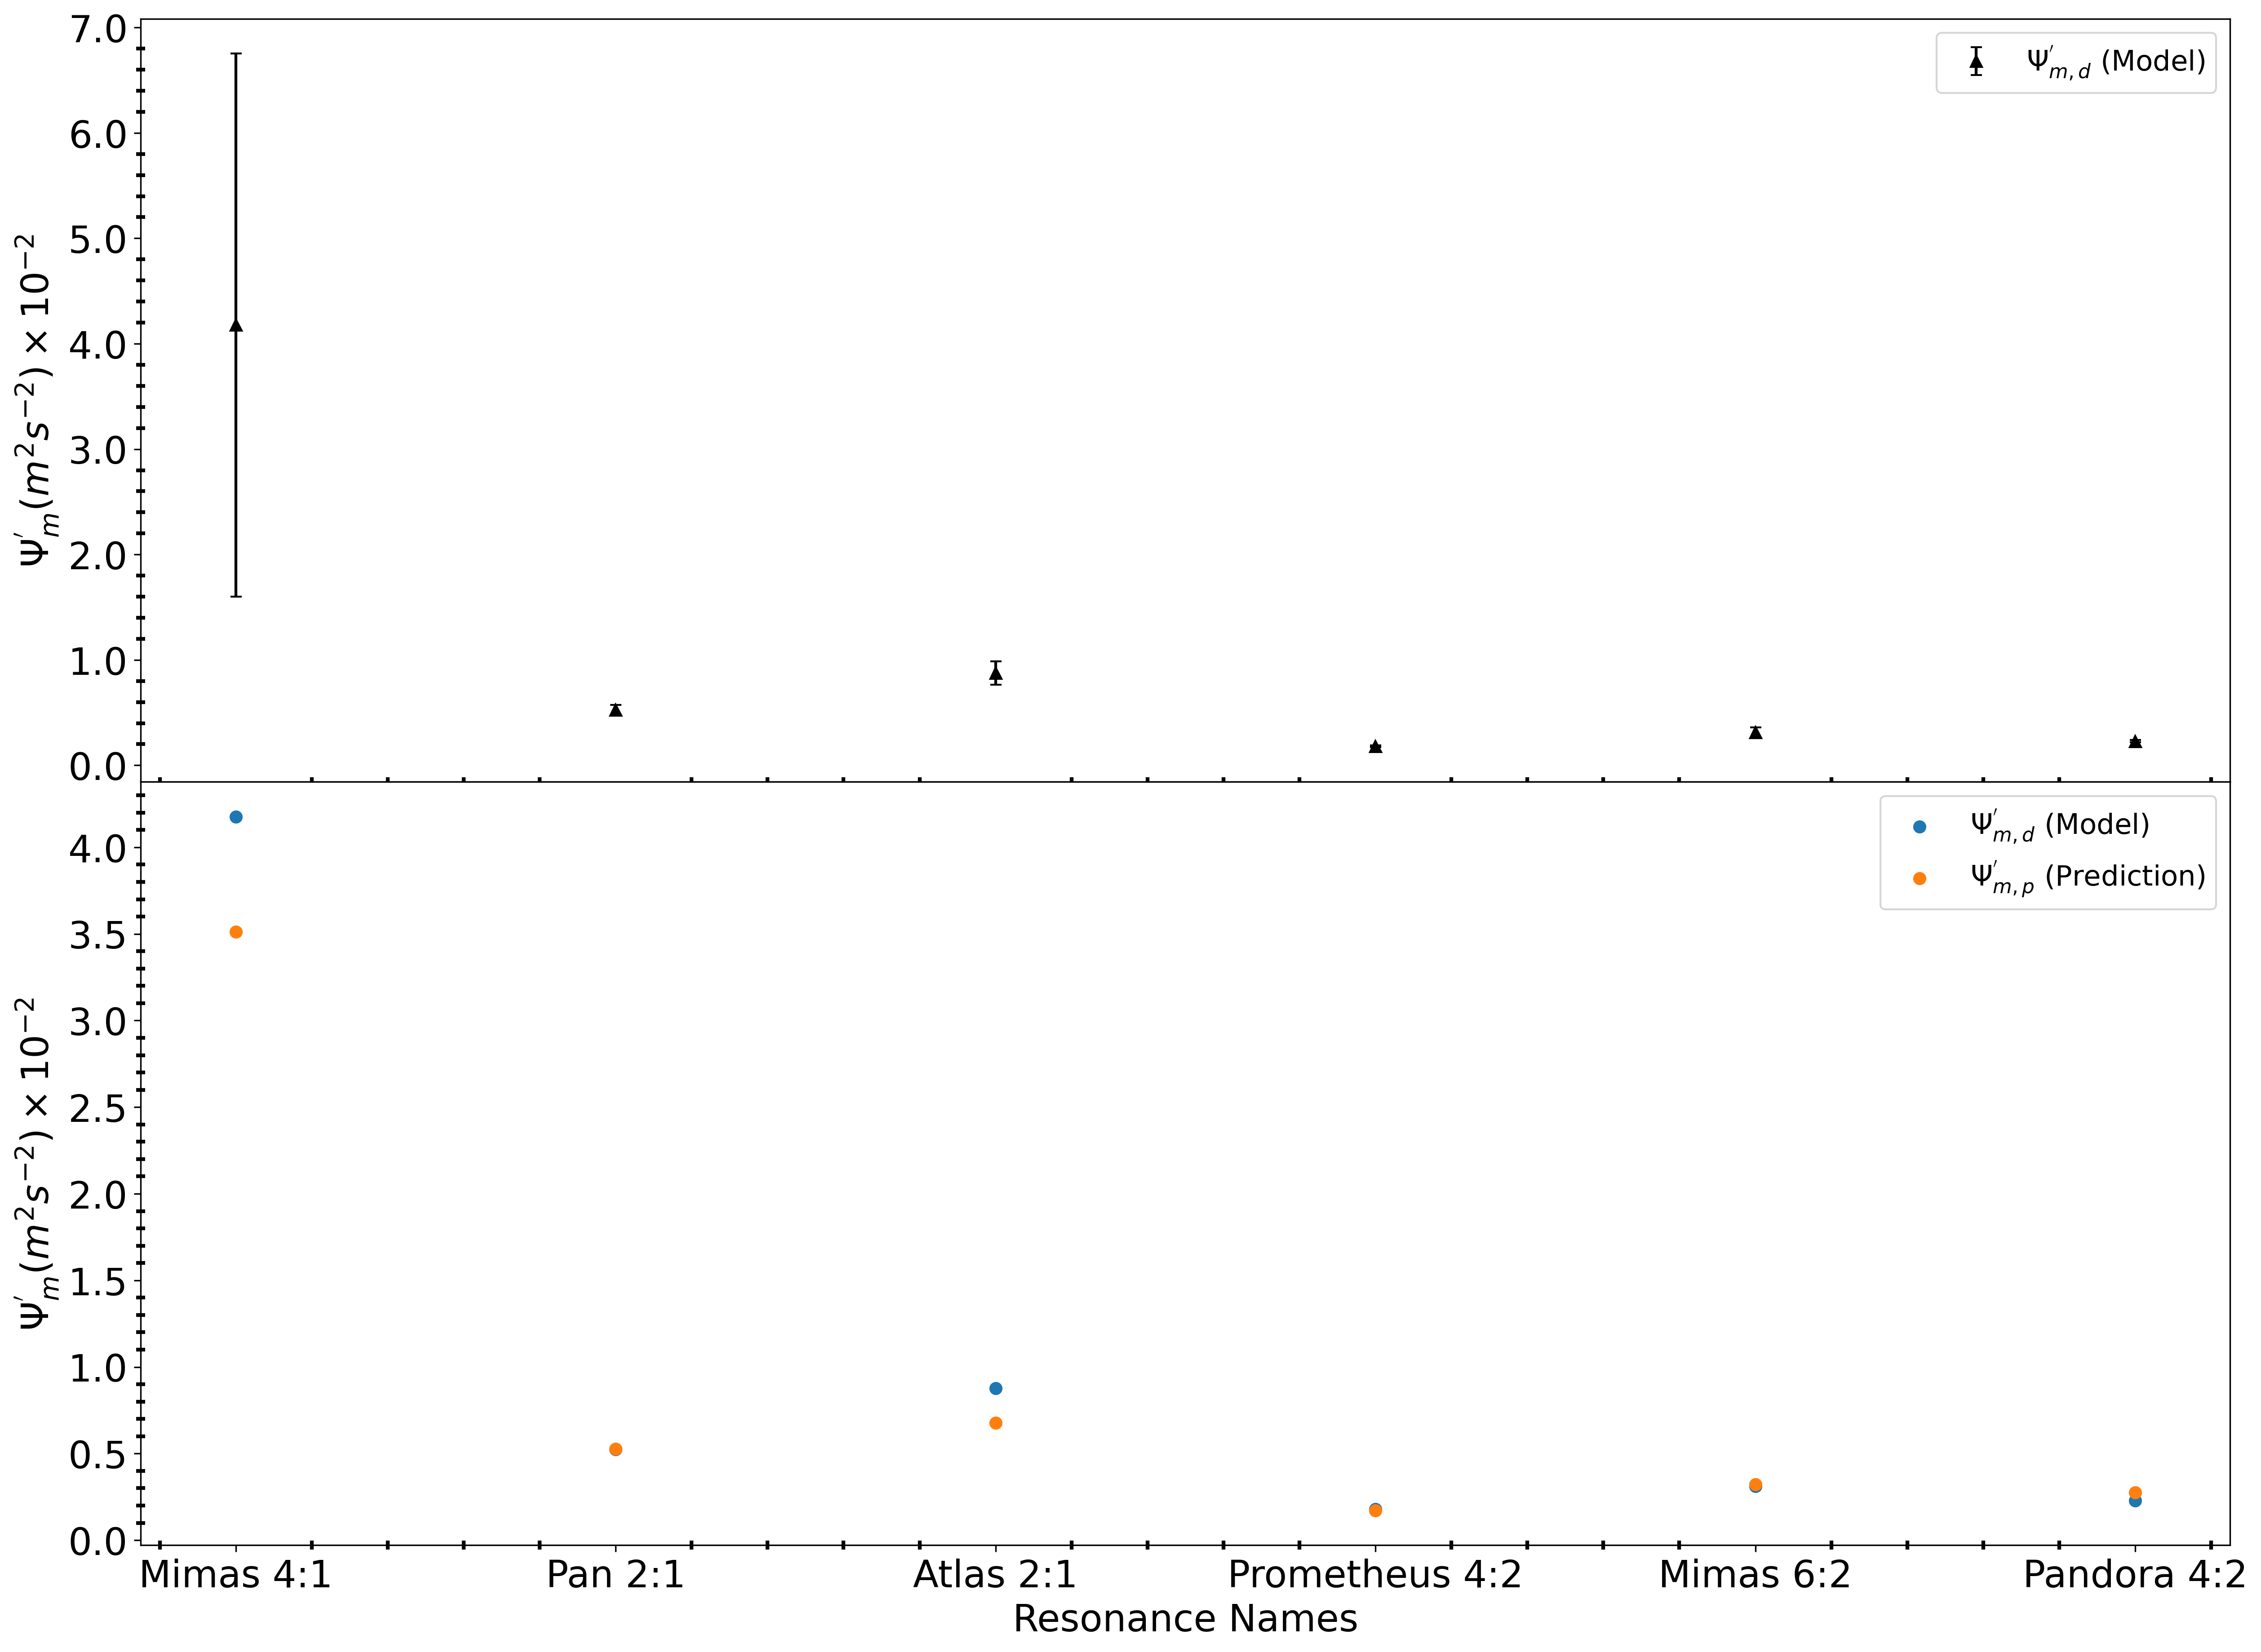
\includegraphics[width=0.8\linewidth]{satellitepotentialUpdated.png}
    \caption{Scatter Plot for calculated and predicted gravitational potential estimates (for satellite waves).}
    \label{fig:enter-label}
\end{figure}

%................../////////////////////////......................////////////////////
\subsection{Preliminary Result II: Applications to non-Satellite Resonances}
In this section, we start by describing the parameters used in the wave-fitting routine.

\subsubsection{Wave-fitting Routine For non-Satellite Resonances}
The Table 8 contains the results for the wave-fitting routine involving non-satellite resonances.

\textbf{Wave ID:} This column simply provides an identifier for each data entry for the spiral density wave. It serves as a reference point for distinguishing between different waves and their corresponding parameters. The encoded numbers are just synonymous with the resonant locations of the waves, while the "Wave" identity is for the waves being analyzed. Each wave likely corresponds to a specific resonance pattern or phenomenon under investigation.

\textbf{Radial Range (Km):} The " Radial Range (Km)" column defines the range of distance in kilometers within which the resonance selection was made. It provides information about the spatial extent of the resonance phenomenon.
    
\textbf{Resonance Location (Km):} This column specifies the precise location of the resonance in kilometers. It indicates where the resonance occurs within the system or environment being studied (with respect to the center of the planet).
    
\textbf{\(l\):} \(l\) represents the angular degree, which characterizes the component of the normal-mode system. It indicates the rotational behavior associated with the resonance.
    
\textbf{\(m\):} The \(m\) column represents the azimuthal order. It describes the orientation or number of spiral arms for the specific density wave influenced by the resonance.
    
\textbf{Pattern Speed (\(^{o}/day\)):} This column specifies the speed of the resonance, measured in degrees per day. It indicates the rate of change of the resonance over time.
    
\textbf{\(a_{fit}\):} \(a_{fit}\) is a fitted parameter obtained from the wave-fitting routine, which represents the dimensionless amplitude of the spiral density wave profile analyzed.
    
\textbf{\(x_{d}\):} \(x_{d}\) is another fitted parameter obtained from the wave-fitting routine, representing the damping parameter. It represents a characteristic distance or position associated with the resonance.
    
\textbf{\(\phi_{0}(rad)\):} This column specifies the initial phase of the wave in radians. It provides information about the starting point or phase offset of the resonance pattern. This could either be positive or negative phase.
    
\textbf{\(x_{r}(Km)\):} \(x_{r}(Km)\) represents the resonant distance offset in kilometers, indicating the corrected distance at which resonance occurs within the system. This could either be positive or negative, depending on the individual wave-fitting routine case.
    
\textbf{\(x_{f}(Km)\):} \(x_{f}(Km)\) denotes the fitted distance in kilometers, known as the winding parameter, obtained through the fitting process. It likely represents a best-fit estimate of the resonant distance based on the data.

\begin{table}[h]
\centering
\vspace{-1.5cm} % Adjust the value as needed for vertical spacing before the table
\rotatebox{90}{
%\normal
\begin{tabular}{|c|c|c|c|c|c|c|c|c|c|c|c|}
\hline
Wave ID & \stackon[0pt]{(Km)}{\stackon[0pt]{Range}{Radial}} & \stackon[0pt]{(Km)}{\stackon[0pt]{Location ($r_{L}$)}{Resonance}} &  $l$ &  $m$ & \stackon[0pt]{$(^{o}/day)$}{\stackon[0pt]{Speed}{Pattern}} & $a_{fit}(Unit)$ & $x_{d}(Unit)$ & $\phi_{0}(rad)$ & $x_{r}(Km)$ & $x_{f}(Km)$ \\
\hline
\stackon[0pt]{Resonance}{\stackon[0pt]{Satellite}} & \saturn & \saturn & \saturn & \saturn & \saturn & \saturn & \saturn & \saturn & \saturn & \saturn \\
\hline

Mimas 4:1 & 74880.00 - 74895.00 & 74890.070 & - & 2 & 762.988 & 0.2229 $\pm$ 0.0305 & 2.7986 $\pm$ 0.0723 & -4.1869 $\pm$ 0.8471 & 2.6125 $\pm$ 1.0523 & 1.5657 $\pm$ 0.2979 \\

Pan 2:1 & 85090.00 - 85130.00 & 85105.020 & - & 2 & 626.032 & 0.0139 $\pm$ 0.0013 & 4.5691 $\pm$ 0.1661 & -6.2832 $\pm$ 2.7684e-12 & 1.1439 $\pm$ 0.0288 & 2.6895 $\pm$ 0.0088 \\

Atlas 2:1 & 87640.00 - 87650.00 & 87645.680 & - & 2 & 598.312 & 0.1684 $\pm$ 0.0200 & 2.2372 $\pm$ 0.0908 & -0.8166 $\pm$ 0.1451 & 0.3621 $\pm$ 0.0346 & 1.0447 $\pm$ 0.0149 \\

Prometheus 4:2 & 88420.00 - 88440.00 & 88434.120 & - & 3 & 782.128 & 0.0067 $\pm$ 0.0003 & 5.8369 $\pm$ 0.0941 & 0.2629 $\pm$ 0.1654 & 0.4764 $\pm$ 0.0652 & 1.6954 $\pm$ 0.0068 \\

Mimas 6:2 & 89870.00 - 89890.00 & 89884.000 & - & 3 & 762.977 & 0.0128 $\pm$ 0.0013 & 4.8527 $\pm$ 0.2113 & -1.7461 $\pm$ 0.8968 & 1.2660 $\pm$ 0.4235 & 1.6616 $\pm$ 0.0572 \\

Pandora 4:2 & 89887.00 - 89897.00 & 89893.680 & - & 3 & 762.852 & 0.0074 $\pm$ 0.0003 & 6.9140 $\pm$ 0.0368 & -3.2364 $\pm$ 0.0662 & 0.2341 $\pm$ 0.0271 & 1.8745 $\pm$ 0.0025 \\

\hline
\stackon[0pt]{Resonance}{\stackon[0pt]{Planetary}} & \saturn & \saturn & \saturn & \saturn & \saturn & \saturn & \saturn & \saturn & \saturn & \saturn \\
\hline

$W74.51^{av}$ & 74501.00 - 74509.00 & 74506.900 & 12 & -8 & 1697.339 & 0.6998 $\pm$ 0.1447 & 2.1436 $\pm$ 0.2624 & -1.6261 $\pm$ 2.9571 & 0.3115 $\pm$ 0.2709 & 0.7179 $\pm$ 0.0745 \\

W74.74 & 74736.00 - 74743.00 & 74739.850 & 15 & 13 & 1390.843 & 0.1723 $\pm$ 0.0274 & 1.7856 $\pm$ 0.1474 &  6.0904 $\pm$ 4.7825 & -0.3983 $\pm$ 0.1299 & 0.3919 $\pm$ 0.0349 \\

W74.75 & 74746.00 - 74748.00 & 74748.300 & 11 & 11 & 1369.932 & 0.2000 $\pm$ 0.0624 & 1.2123 $\pm$ 0.1070 & -1.7116 $\pm$ 0.2681 & 0.0687 $\pm$ 0.2258 & 0.9133 $\pm$ 0.1862 \\

W74.76 & 74752.00 - 74762.00 & 74756.600 & 19 & -11 & 1638.389 & 0.2000 $\pm$ 0.0154 & 1.4920 $\pm$ 0.0744 & -0.8651 $\pm$ 0.1511 & -0.0497 $\pm$ 0.0114 & 0.3314 $\pm$ 0.0040 \\
         
W75.14 & 75142.00 - 75144.00 & 75143.000 & 16 & -10 & 1638.983 & 0.2774 $\pm$ 0.0311 & 1.7827 $\pm$ 0.1049 &  0.8276 $\pm$ 0.5898 & 0.4986 $\pm$ 0.1000 & 0.5114 $\pm$ 0.0339 \\

W76.02A & 76016.00 - 76018.00 & 76018.100 & 13 & -9 & 1626.530 & 0.5711 $\pm$ 0.0763 & 1.9183 $\pm$ 0.0596 & 1.4200 $\pm$ 0.1741 & 0.7562 $\pm$ 0.0546 & 0.9157 $\pm$ 0.0231 \\

W76.44 & 76433.00 - 76436.00 & 76435.400 & 2 & -2 & 2169.260 & 0.2265 $\pm$ 0.0343 & 2.5640 $\pm$ 0.1227 & -1.3821 $\pm$ 0.1955 & 0.1697 $\pm$ 0.0969 & 0.9200 $\pm$ 0.0248 \\
    
$W76.46^{av}$ & 76457.00 - 76462.00 & 76459.500 & 9 & -7 & 1657.720 & 0.1716 $\pm$ 0.0318 & 2.4535 $\pm$ 0.1146 & -0.3696 $\pm$ 0.4269 & 0.1361 $\pm$ 0.0598 & 0.5913 $\pm$ 0.0132 \\
         
W77.34 & 77337.00 - 77339.00 & 77338.900 & 14 & -10 & 1569.078 & 0.1590 $\pm$ 0.0141 & 2.2988 $\pm$ 0.0356 & -1.6487 $\pm$ 0.0668 & 0.1711 $\pm$ 0.0299 & 0.5362 $\pm$ 0.0119 \\

W78.51 & 78503.00 - 78509.00 & 78506.750 & 15 & -11 & 1521.410 & 0.3983 $\pm$ 0.0350 & 1.7636 $\pm$ 0.0614 &  -1.0069 $\pm$ 0.1360 & 0.0743 $\pm$ 0.0275 & 0.6044 $\pm$ 0.0141 \\

W79.04 & 79039.00 - 79045.00 & 79042.300 & 11 & -9 & 1533.336 & 0.0888 $\pm$ 0.0122 & 2.5361 $\pm$ 0.1297 & -3.8004 $\pm$ 0.1893 & 0.2564 $\pm$ 0.0671 & 0.7877 $\pm$ 0.0200 \\

W79.55 & 79546.00 - 79550.00 & 79548.920 & 16 & -12 & 1481.152 & 0.0704 $\pm$ 0.0234 & 2.4876 $\pm$ 0.2693 &  -2.1020 $\pm$ 0.8213 & 0.2901 $\pm$ 0.2261 & 0.6299 $\pm$ 0.0481 \\

W80.49 & 80484.00 - 80488.00 & 80486.100 & 17 & -13 & 1446.654 & 0.0515 $\pm$ 0.0112 & 2.0756 $\pm$ 0.3069 &  -3.3740 $\pm$ 0.9352 & -0.2457 $\pm$ 0.3462 & 0.6728 $\pm$ 0.0840 \\

W80.99 & 80983.00 - 80989.00 & 80986.150 & 4 & -4 & 1660.363 & 0.1700 $\pm$ 0.0042 & 3.4683 $\pm$ 0.0364 &  -3.2070 $\pm$ 0.0901 & 0.2585 $\pm$ 0.0361 & 1.5753 $\pm$ 0.0046 \\

W81.023A & 81018.00 - 81030.00 & 81023.100 & 5 & -5 & 1593.630 & 0.0444 $\pm$ 0.0062 & 3.0357 $\pm$ 0.1988 &  -1.7460 $\pm$ 1.0195 & -0.1003 $\pm$ 0.4762 & 1.1562 $\pm$ 0.0928 \\

W81.024B & 81018.00 - 81030.00 & 81024.150 & 13 & -11 & 1450.495 & 0.0582 $\pm$ 0.0024 &  2.8770 $\pm$ 0.0803 & -1.0586 $\pm$ 0.0564 & 0.4178 $\pm$ 0.0396 & 0.9040 $\pm$ 0.0100 \\
         
W81.33 & 81333.00 - 81336.00 & 81334.275 & 18 & -14 & 1416.734 & 0.0378 $\pm$ 0.0025 & 2.1450 $\pm$ 0.1614 & -5.7389 $\pm$ 0.7457 & -0.2744 $\pm$ 0.3107 & 0.5961 $\pm$ 0.0897 \\

W81.43 & 81420.00 - 81430.00 & 81429.550 & 6 & -6 & 1538.237 & 0.0197 $\pm$ 0.0042 & 2.6979 $\pm$ 0.2250 &  2.1297 $\pm$ 1.1163 & 0.7173 $\pm$ 0.5615 & 1.2245 $\pm$ 0.1165 \\

W81.96 & 81959.00 - 81965.00 & 81962.450 & 7 & -7 & 1492.457 & 0.0299 $\pm$ 0.0024 & 2.8510 $\pm$ 0.1394 &  3.0115 $\pm$ 0.8872 & -0.9500 $\pm$ 0.3823 & 1.0838 $\pm$ 0.0674 \\

W82.01 & 82004.00 - 82009.00 & 82007.750 & 3 & -3 & 1736.645 & 0.1009 $\pm$ 0.0013 & 3.7871 $\pm$ 0.0096 &   -0.7900 $\pm$ 0.0265 & -0.2765 $\pm$ 0.0214 & 1.9368 $\pm$ 0.0045 \\
         
W82.06 & 82055.00 - 82065.00 & 82059.400 & 3 & -3 & 1734.999 & 0.2113 $\pm$ 0.0035 & 3.7659 $\pm$ 0.0351 &  -0.9592 $\pm$ 0.1470 & 0.2273 $\pm$ 0.1551 & 2.5483 $\pm$ 0.0287 \\

W82.21 & 82187.50 - 82207.51 & 82207.500 & 3 & -3 & 1730.293 & 0.2536 $\pm$ 0.0046 & 3.5938 $\pm$ 0.0536 &  -0.8110 $\pm$ 0.0633 & 0.4772 $\pm$ 0.0731 & 1.9758 $\pm$ 0.0167 \\

W82.53 & 82510.00 - 82530.00 & 82528.750 & 8 & -8 & 1454.224 & 0.0109 $\pm$ 0.0029 & 3.4632 $\pm$ 0.3486 &  0.5753 $\pm$ 2.7935 & 0.2177 $\pm$ 0.0556 & 1.0787 $\pm$ 0.0202 \\

W82.61 & 82606.00 - 82608.00 & 82607.750 & 15 & -13 & 1390.843 & 0.0214 $\pm$ 0.0028 & 2.6706 $\pm$ 0.0938 &  -1.6706 $\pm$ 0.2270 & 0.5028 $\pm$ 0.0966 & 1.0285 $\pm$ 0.0151 \\
         
W83.09 & 83086.00 - 83096.00 & 83090.650 & 9 & -9 & 1421.844 & 0.0402 $\pm$ 0.0010 & 2.8967 $\pm$ 0.0856 &  -4.0353 $\pm$ 0.1450 & -0.2088 $\pm$ 0.0609 & 1.1950 $\pm$ 0.0118 \\

W83.63 & 83612.02 - 83637.02 & 83632.020 & 10 & -10 & 1394.056 & 0.2737 $\pm$ 0.0113 & 2.6295 $\pm$ 0.0469 & -0.9169 $\pm$ 0.0708 & 0.3456 $\pm$ 0.0262 & 1.0516 $\pm$ 0.0038 \\

W84.15 & 84140.00 - 84150.00 & 84147.100 & 11 & -11 & 1369.910 & 0.0137 $\pm$ 0.0016 & 3.1846 $\pm$ 0.1332 & -5.2746 $\pm$ 0.4688 & 0.2660 $\pm$ 0.1842 & 0.9899 $\pm$ 0.0339 \\

W84.64 & 84630.00 - 84650.00 & 84643.200 & 2 & -2 & 1860.752 & 0.1829 $\pm$ 0.0037 & 3.9257 $\pm$ 0.0402 &  1.2049 $\pm$ 0.0867 & 0.3505 $\pm$ 0.0874 & 2.0115 $\pm$ 0.0152 \\

W87.19 & 87170.00 - 87210.00 & 87192.800 & 2 & -2 & 1779.548 & 0.0494 $\pm$ 0.0017 & 5.2729 $\pm$ 0.0468 & -4.3997 $\pm$ 2.6259 & 0.3902 $\pm$ 0.0882 & 1.8039 $\pm$ 0.0106 \\

\hline
\end{tabular}
\vspace{-1.5cm} % Adjust the value as needed for vertical spacing after the table
}
\caption{Data for Wave-fitting routine for satellite and non-satellite resonances.}
\end{table}


\subsubsection{Model Computation for Ring Properties using non-Satellite Resonances:}

\paragraph{Optical Depth ($\tau_{av}$):}
From figure 16, we have a panel which shows four plots corresponding to the key properties of Saturn's C-Ring. The continuous plot with the blue line at the top of the panel represents the complete optical depth profile for the extent of the ring, given between 74000 Km to 90000 Km. While the black and red scatter plots represent data from planetary and satellite resonances, respectively. The trend clearly shows an increase in optical(average) depth as per our archived wave signals. 

The average optical depth characterizes the opacity of the C-ring to radiation, mostly visible light. It quantifies the extent to which light is absorbed or scattered as it passes through the ring. Higher values of $\tau_{av}$ indicate greater opacity, suggesting more efficient absorption or scattering of light within the C-ring, while lower values of $\tau_{av}$ indicate more transparent regions of the particular planetary ring under investigation.

Statistically, the average optical depth of approximately 0.102 for Saturn's C-Ring suggests that, on average, the particles within the ring are relatively transparent, allowing some light to pass through but not completely transparent. A moderate standard deviation of 0.078 indicates that while the average optical depth is around 0.102, there is variability in the opacity of different parts of the C-Ring. This variability could be due to variations in particle density or size within the ring. The range from approximately 0.028 to 0.361 indicates that there are areas within the C-Ring where the optical depth is significantly lower or higher than the average. The minimum value suggests areas where the ring is relatively transparent, while the maximum value suggests regions of higher opacity, potentially due to denser particle concentrations or different particle compositions. Based on the quartile values, 25 percent of the observations have an optical depth value below approximately 0.048. The median optical depth value (50th percentile) is around 0.088, indicating that half of the observations have optical depth values below this value, while 75 percent of the observations have an optical depth value below approximately 0.117. The quartile values provide insights into the distribution of optical depth values within the C-Ring. The 25th percentile (Q1) and 75th percentile (Q3) values indicate the range in which the majority of the data falls, with the median (50th percentile) representing the middle point of this distribution. 

Overall, these observations suggest that Saturn's C-Ring exhibits variability in opacity, with areas of relatively low and high optical depth. Further analysis could be conducted to investigate the factors influencing this variability, such as particle size distribution, composition, or external influences such as gravitational forces.

\paragraph{Surface Mass Density ($\sigma_{0}$):}
Surface mass density represents the amount of mass per unit area at the surface of the C-ring. Variations in $\sigma_{0}$ reflect differences in the density and distribution of ring material. The second row from the panel of plot in figure 16, shows the trends of values which indicate the spatial heterogeneity of the C-ring, with some regions being denser than others. 

Generally, between 74000 Km and around 82000 Km, there is a trend of increase in surface mass density distribution with a gradient of roughly around $1.613 g/cm^{2}$ per Km. There are notable high points around 75000 Km and 82000 Km, with the latter showing the highest peak value, which might imply the region along the C-Ring with the highest distribution of mass per area. Beyond 82000 Km, there is a somewhat steady decrease in surface mass density distribution with an average magnitude of roughly $1.46g/cm^{2}$ per Km, except for the gap within the radial range of 85000 Km to 87000 Km.

By analyzing 35 wave samples (satellite and planetary resonances), we observed the following results on the distribution of mass within Saturn's C-Ring. The average density of $2.49 g/cm^{2}$ provides a baseline understanding of the typical mass per unit area within the ring, while the standard deviation of $1.51 g/cm^{2}$ suggests that the C-Ring is not uniform in density. There are regions with significantly lower or higher density compared to the average. The minimum and maximum values highlight the significant variation in mass density across the C-Ring. Some areas have densities as low as $0.25 g/cm^{2}$, while others reach up to around $7.77 g/cm^{2}$. The quartile values (25 percent and 75 percent) provide information about how the data is spread.  For instance, 75 percent of the measurements fall below $3.31 g/cm^{2}$, indicating that a large portion of the C-Ring has a mass density below this value.

This data analysis paves the way for further investigation into the factors influencing the variability of mass density within the C-Ring.

\textbf{Particle Composition:} The types of materials making up the ring particles could influence their mass density. Denser materials like water ice would contribute to higher mass density regions, while less dense materials like porous dust might be found in lower density areas.

\textbf{Particle Size and Distribution:}  Variations in particle size and how they are distributed within the C-Ring could also play a role. Larger, more massive particles might be concentrated in specific regions, leading to higher densities.

\textbf{Gravitational Interactions:} The gravitational influence of Saturn and its moons could potentially affect the distribution of mass within the C-Ring. Regions experiencing stronger gravitational forces might have a more tightly packed structure, resulting in higher density.


\paragraph{Mass Extinction Coefficient ($\kappa$):}
The mass extinction coefficient quantifies the efficiency of light extinction per unit mass of the C-ring material. It combines the effects of absorption and scattering of light. Higher values of $\kappa$ suggest that the C-ring material is more effective at extinguishing light per unit mass.

To start with, the third (semi-log) plot in the panel shows the results for the mass extinction coefficient ($\kappa$), versus the radial range of the C-ring containing majority of the waves detected. The trend for mass extinction coefficient($\kappa$) shows some aliquot amount of instability between the radial range of 74000 Km to 85000 Km, with a fitted slope of around 0.04 per Km, except for the gap-region between 85000 Km and around 87000 Km where there a no wave signals detected. Such region corresponds with the elevated areas of the C-ring optical depth. Beyond, say 87000 Km, there is a noticeable increase in mass extinction coefficient. This implies that between the radial range of 74000 Km to 85000 Km, the C-ring is mostly populated by materials with higher radii compare to regions between 87000 Km to 90000 Km, which are populated by materials with smaller radii. 

An exploratory data analysis for the mass extinction coefficient, measured in \( \text{cm}^2/\text{g} \), provides valuable insights into the distribution and characteristics of this property within Saturn's C-Ring. A detailed interpretation is found below.

Considering the 35 observations in the dataset, indicating the sample size, the mean mass extinction coefficient is \(0.058148 \, \text{cm}^2/\text{g}\), which represents the average value of the mass extinction coefficient across all observations. The standard deviation of \(0.070492 \, \text{cm}^2/\text{g}\) indicates the degree of dispersion or variability of the mass extinction coefficient values around the mean. The relatively high standard deviation suggests that the data points are widely spread out from the mean, indicating significant variability in the scattering and absorption properties of the particles within the C-Ring. The minimum and maximum mass extinction coefficient values are \(0.008173 \, \text{cm}^2/\text{g}\) and \(0.296640 \, \text{cm}^2/\text{g}\), respectively. This indicates a wide range of variation in the scattering and absorption properties of the particles within the C-Ring. The presence of such a broad range of values suggests some form of heterogeneity in the composition, size, and spatial distribution of the particles within the ring. The \(25^{th}\) percentile (Q1) is \(0.027268 \, \text{cm}^2/\text{g}\), indicating that \(25\%\) of the observations have a mass extinction coefficient value below this threshold, while the median (or \(50^{th}\) percentile, Q2) is \(0.033066 \, \text{cm}^2/\text{g}\), representing the middle value of the data set. This indicates that \(50\%\) of the observations have a mass extinction coefficient value below this value; the \(75^{th}\) percentile (Q3) is \(0.044598 \, \text{cm}^2/\text{g}\), indicating that \(75\%\) of the observations have a mass extinction coefficient value below this threshold. These statistics collectively suggest a significant variation of the mass extinction coefficient of Saturn's C-Ring across different regions, indicating variations in particle size, composition, and density within the ring.


\paragraph{Viscosity Estimates ($\nu$):}
Figure 16d shows the semi-log plot for the kinematic viscosity estimates ($\nu$) derived from equation 57, versus the radial extent of the C-Ring, showing a somewhat consistent trend of decrease over the radial range of 74000 Km to 90000 Km, with a negative slope of around 0.098690 per Km: between 74000 Km and 85000 Km, the is a slightly stable decrease in the kinematic viscosity from a high point above 100.00 units to a low point around 10.00 unit, on the semi-log plot. The gap-region is currently unjustifiable and does not contain enough information to fit the current trend for the result. Regions between 87000 Km to 90000 Km are characterized by another steep descent in viscosity, from around 0.50 to around 0.1 on the semi-log plot.

From \cite{araki1986dynamics, Dougherty2009SaturnFC, 1988AJ.....95..925W}, we derive a fundamental relationship shedding light on the interplay between kinematic viscosity and the root-mean-square (rms) random velocity, denoted as $c$, of particles within Saturn's rings. This relationship is expressed mathematically as:
\begin{equation}
    \nu = k_{1}\frac{c^{2}}{\Omega}\left(\frac{\tau}{1+\tau^{2}}\right) + k_{2}\Omega D^{2}\tau,
\end{equation}
Here, $\nu$ signifies the kinematic viscosity, $\tau$ represents the local optical depth, $\Omega$ stands for the orbital frequency, and $D$ denotes the particle diameter. The constants $k_{1}$ and $k_{2}$ are characteristic coefficients typically on the order of unity.

This equation reveals a connection: regions characterized by higher kinematic viscosity tend to exhibit higher root-mean-square random velocities of ring particles ($c$), whereas regions with lower kinematic viscosity tend to manifest lower random velocities. This observation aligns with comprehensive optical depth profiles given in the first plot. For instance, in regions like 74000 km to 85000 km, characterized by more stable plateaus, an abundance of ring particles facilitates increased interactions among themselves, consequently augmenting their random velocities. Conversely, in less stable-plateau regions, such as 87000 km to 90000 km, fewer particle interactions occur, leading to diminished random velocities due to decreased kinematic viscosity. This dynamic interplay underscores the complex relationship between kinematic viscosity and particle dynamics within Saturn's C-Ring, which might shed more light on the intricate mechanisms governing their behavior.

Our analysis of 35 kinematic viscosity measurements within the extent of Saturn's C-Ring reveals intriguing details about the region's particles' behavior. The average viscosity of $23.49cm^{2}/s$ indicates the typical rate of fluid flow per unit area. However, a standard deviation of $39.33cm^{2}/s$ points to significant variations across the data, suggesting the C-Ring's fluidity is not uniform. This variability is further highlighted by the wide range of viscosity values, from a low of $1.38cm^{2}/s$ to a high of $236.57cm^{2}/s$. Additionally, quartile analysis shows that the lower half of the data falls below $7.25cm^{2}/s$, while the upper half falls below $23.52cm^{2}/s$. The median viscosity of $14.81cm^{2}/s$ reinforces the notion of a broad spectrum of fluid flow behaviors within the C-Ring. These findings suggest that factors like particle size distribution, temperature variations, and gravitational interactions with moons might influence viscosity patterns within the C-Ring. Further investigation into these factors could shed light on the mechanisms behind the observed variability, leading to a more comprehensive understanding of the ring's fluid dynamics.

Saturn's C-Ring particles do not have a simple viscosity value. They behave like a very slow-moving fluid: collisions between particles and the influence of Saturn's gravity create a slight resistance to changes in their motion. This resistance is similar to viscosity in a fluid. The trends from the results might show that the C-Ring materials are more fluffy around 87000 Km to 90000Km, and less fluffy at other regions. The particles' gravity may be the main contributor to the overall viscosity, as it is especially in the denser A ring\cite{https://doi.org/10.1029/2005GL025163}.


% DATA FOR TAU_AV + SIGMA + KAPPA + VISCOSITY

\begin{table}[h]
\centering
\vspace{-1.5cm} % Adjust the value as needed for vertical spacing before the table
\rotatebox{90}{
%\normal
\begin{tabular}{|c|c|c|c|c|c|c|c|c|c|}
\hline
Wave ID & \stackon[0pt]{(Km)}{\stackon[0pt]{Range}{Radial}} & \stackon[0pt]{(Km)}{\stackon[0pt]{Location ($r_{L}$)}{Resonance}} & $l$ & $m$ & $\tau_{av}$ & $\sigma_{0} (g/cm^{2})$ & $\kappa = \frac{\tau_{av}}{\sigma_{0}} (cm^{2}/g)$ & $\nu (cm^{2}/s)$\\
\hline
\stackon[0pt]{Resonance}{\stackon[0pt]{Satellite}} & \saturn & \saturn & \saturn & \saturn & \saturn & \saturn & \saturn & \saturn \\
\hline
Mimas 4:1 & 74880.00 - 74895.00 & 74890.070 & - & 2 & 0.034336 & 1.057663 $\pm$ 0.402423 & 0.032464 $\pm$ 0.012352 & 9.483924 $\pm$ 5.462388 \\
Pan 2:1 & 85090.00 - 85130.00 & 85105.020 & - & 2 & 0.082371 & 1.871221 $\pm$ 0.012231 & 0.044020 $\pm$ 0.000288 & 8.041822 $\pm$ 0.880359 \\
Atlas 2:1 & 87640.00 - 87650.00 & 87645.680 & - & 2 & 0.061705 & 0.250998 $\pm$ 0.007156 & 0.245840 $\pm$ 0.007009 & 3.732417 $\pm$ 0.481570 \\
Prometheus 4:2 & 88420.00 - 88440.00 & 88434.120 & - & 3 & 0.241621 & 1.275612 $\pm$ 0.010282 & 0.189415 $\pm$ 0.001527 & 1.768575 $\pm$ 0.088186 \\
Mimas 6:2 & 89870.00 - 89890.00 & 89884.000 & - & 3 & 0.340543 & 1.148003 $\pm$ 0.079018 & 0.29664 $\pm$ 0.020418 & 2.781585 $\pm$ 0.463107 \\
Pandora 4:2 & 89887.00 - 89897.00 & 89893.680 & - & 3 & 0.361360 & 1.460548 $\pm$ 0.003932 & 0.247414 $\pm$ 0.000666 & 1.380620 $\pm$ 0.022726 \\
\hline
\stackon[0pt]{Resonance}{\stackon[0pt]{Planetary}} & \saturn & \saturn & \saturn & \saturn & \saturn & \saturn & \saturn & \saturn \\
\hline
$W74.51^{av}$ & 74501.00 - 74509.00 & 74506.900 & 12 & -8 & 0.055950 & 2.042644 $\pm$ 0.424109 & 0.027391 $\pm$ 0.005687 & 18.853480 $\pm$ 9.077400 \\

W74.74 & 74736.00 - 74743.00 & 74739.850 & 15 & 13 & 0.036219 & 0.801756 $\pm$ 0.142944 & 0.045175 $\pm$ 0.008054 & 7.025685 $\pm$ 2.560542 \\

W74.75 & 74746.00 - 74748.00 & 74748.300 & 11 & 11 & 0.029636 & 3.625972 $\pm$ 1.478684 & 0.008173 $\pm$ 0.003333 & 236.570543 $\pm$ 157.696303 \\

W74.76 & 74752.00 - 74762.00 & 74756.600 & 19 & -11 & 0.027992 & 0.572831 $\pm$ 0.013839 & 0.048866 $\pm$ 0.001181 & 7.278997 $\pm$ 1.120804 \\

W75.14 & 75142.00 - 75144.00 & 75143.000 & 16 & -10 & 0.029031 & 1.224586 $\pm$ 0.162585 & 0.023707 $\pm$ 0.003148 & 14.181319 $\pm$ 3.774694 \\
        
W76.02A & 76016.00 - 76018.00 & 76018.100 & 13 & -9 & 0.049630 & 3.407717 $\pm$ 0.172025 & 0.014564 $\pm$ 0.000735 & 57.687030 $\pm$ 6.930285 \\

W76.44 & 76433.00 - 76436.00 & 76435.400 & 2 & -2 & 0.029827 & 1.009590 $\pm$ 0.054527 & 0.029544 $\pm$ 0.001596 & 7.219514 $\pm$ 1.190432 \\
    
$W76.46^{av}$ & 76457.00 - 76462.00 & 76459.500 & 9 & -7 & 0.030282 & 1.110717 $\pm$ 0.049593 & 0.027264 $\pm$ 0.001217 & 5.850474 $\pm$ 0.908774 \\
         
W77.34 & 77337.00 - 77339.00 & 77338.900 & 14 & -10 & 0.040235 & 1.199843 $\pm$ 0.053105 & 0.033534 $\pm$ 0.001484 & 7.092551 $\pm$ 0.574918 \\

W78.51 & 78503.00 - 78509.00 & 78506.750 & 15 & -11 & 0.047065 & 1.566088 $\pm$ 0.072900 & 0.030053 $\pm$ 0.001399 & 23.633482 $\pm$ 2.970882 \\

W79.04 & 79039.00 - 79045.00 & 79042.300 & 11 & -9 & 0.078261 & 2.157270 $\pm$ 0.109815 & 0.036278 $\pm$ 0.001847 & 14.408114 $\pm$ 2.469182 \\
         
W79.55 & 79546.00 - 79550.00 & 79548.920 & 16 & -12 & 0.072853 & 1.748319 $\pm$ 0.266793 &  0.041670 $\pm$ 0.006359 & 9.993651 $\pm$ 3.971079 \\
         
W80.49 & 80484.00 - 80488.00 & 80486.100 & 17 & -13 & 0.101275 & 2.049558 $\pm$ 0.512051 & 0.049413 $\pm$ 0.012345 & 21.921085 $\pm$ 12.728644 \\

W80.99 & 80983.00 - 80989.00 & 80986.150 & 4 & -4 & 0.104347 & 3.914558 $\pm$ 0.023021 & 0.026656 $\pm$ 0.000157 & 21.162051 $\pm$ 0.691595 \\

W81.023A & 81018.00 - 81030.00 & 81023.100 & 5 & -5 & 0.102109 & 2.525872 $\pm$ 0.405641 & 0.040425 $\pm$ 0.006492 & 14.964272 $\pm$ 4.651246 \\

W81.024B & 81018.00 - 81030.00 & 81024.150 & 13 & -11 & 0.102109 & 3.088057 $\pm$ 0.068118 & 0.033066 $\pm$ 0.000729 & 16.826878 $\pm$ 1.514519 \\

W81.33 & 81333.00 - 81336.00 & 81334.275 & 18 & -14 & 0.086512 & 1.652931 $\pm$ 0.497447 & 0.052339 $\pm$ 0.015751 & 14.416529 $\pm$ 7.276442 \\

W81.43 & 81420.00 - 81430.00 & 81429.550 & 6 & -6 & 0.094085 & 3.239715 $\pm$ 0.616404 & 0.029041 $\pm$ 0.005526 & 29.184327 $\pm$ 11.076517 \\

W81.96 & 81959.00 - 81965.00 & 81962.450 & 7 & -7 & 0.120603 & 2.825534 $\pm$ 0.351220 & 0.042683 $\pm$ 0.005306 & 19.281665 $\pm$ 4.573847 \\

W82.01 & 82004.00 - 82009.00 & 82007.750 & 3 & -3 & 0.153753 & 4.502252 $\pm$ 0.020979 &  0.034150 $\pm$ 0.000159 & 23.400998 $\pm$ 0.241861 \\

W82.06 & 82055.00 - 82065.00 & 82059.400 & 3 & -3 & 0.131704 & 7.77442 $\pm$ 0.175027 & 0.016941 $\pm$ 0.000381 & 54.118157 $\pm$ 2.372218 \\

W82.21 & 82187.50 - 82207.51 & 82207.500 & 3 & -3 & 0.119105 & 4.639812 $\pm$ 0.078567 &  0.025670 $\pm$ 0.000435 & 28.893884 $\pm$ 1.485897 \\
         
W82.53 & 82510.00 - 82530.00 & 82528.750 & 8 & -8 & 0.105020 & 3.063460 $\pm$ 0.114483 & 0.034281 $\pm$ 0.001281 & 11.731227 $\pm$ 3.603032 \\

W82.61 & 82606.00 - 82608.00 & 82607.750 & 15 & -13 & 0.114571 & 4.315586 $\pm$ 0.126316 & 0.026548 $\pm$ 0.000777 & 34.433086 $\pm$ 3.931101 \\
         
W83.09 & 83086.00 - 83096.00 & 83090.650 & 9 & -9 & 0.127997 & 4.065678 $\pm$ 0.080627 & 0.031482 $\pm$ 0.000624 & 29.780509 $\pm$ 2.784707 \\
         
W83.63 & 83612.02 - 83637.02 & 83632.020 & 10 & -10 & 0.084198 & 3.374606 $\pm$ 0.024093 &  0.024950 $\pm$ 0.000178 & 29.366600 $\pm$ 1.603583 \\
         
W84.15 & 84140.00 - 84150.00 & 84147.100 & 11 & -11 & 0.102993 & 3.182960 $\pm$ 0.218083 & 0.032358 $\pm$ 0.002217 & 14.814989 $\pm$ 2.403297 \\
         
W84.64 & 84630.00 - 84650.00 & 84643.200 & 2 & -2 & 0.087528 & 3.209390 $\pm$ 0.048403 & 0.027273 $\pm$ 0.000411 & 16.286891 $\pm$ 0.621132 \\
         
W87.19 & 87170.00 - 87210.00 & 87192.800 & 2 & -2 & 0.196865 & 2.292140 $\pm$ 0.027028 & 0.085887 $\pm$ 0.001013 & 4.500236 $\pm$ 0.143787 \\

\hline
\end{tabular}
\vspace{-1.5cm}
}
\caption{Data table for Average optical depth, surface mass density mass extinction coefficient and viscosity for satellite and non-Satellite resonances.}
\end{table}

% Corresponding Plot For Surface Mass Density and Mass Extinction Coefficient values for non-Satellite resonances.
\begin{figure}[h]
    \centering
    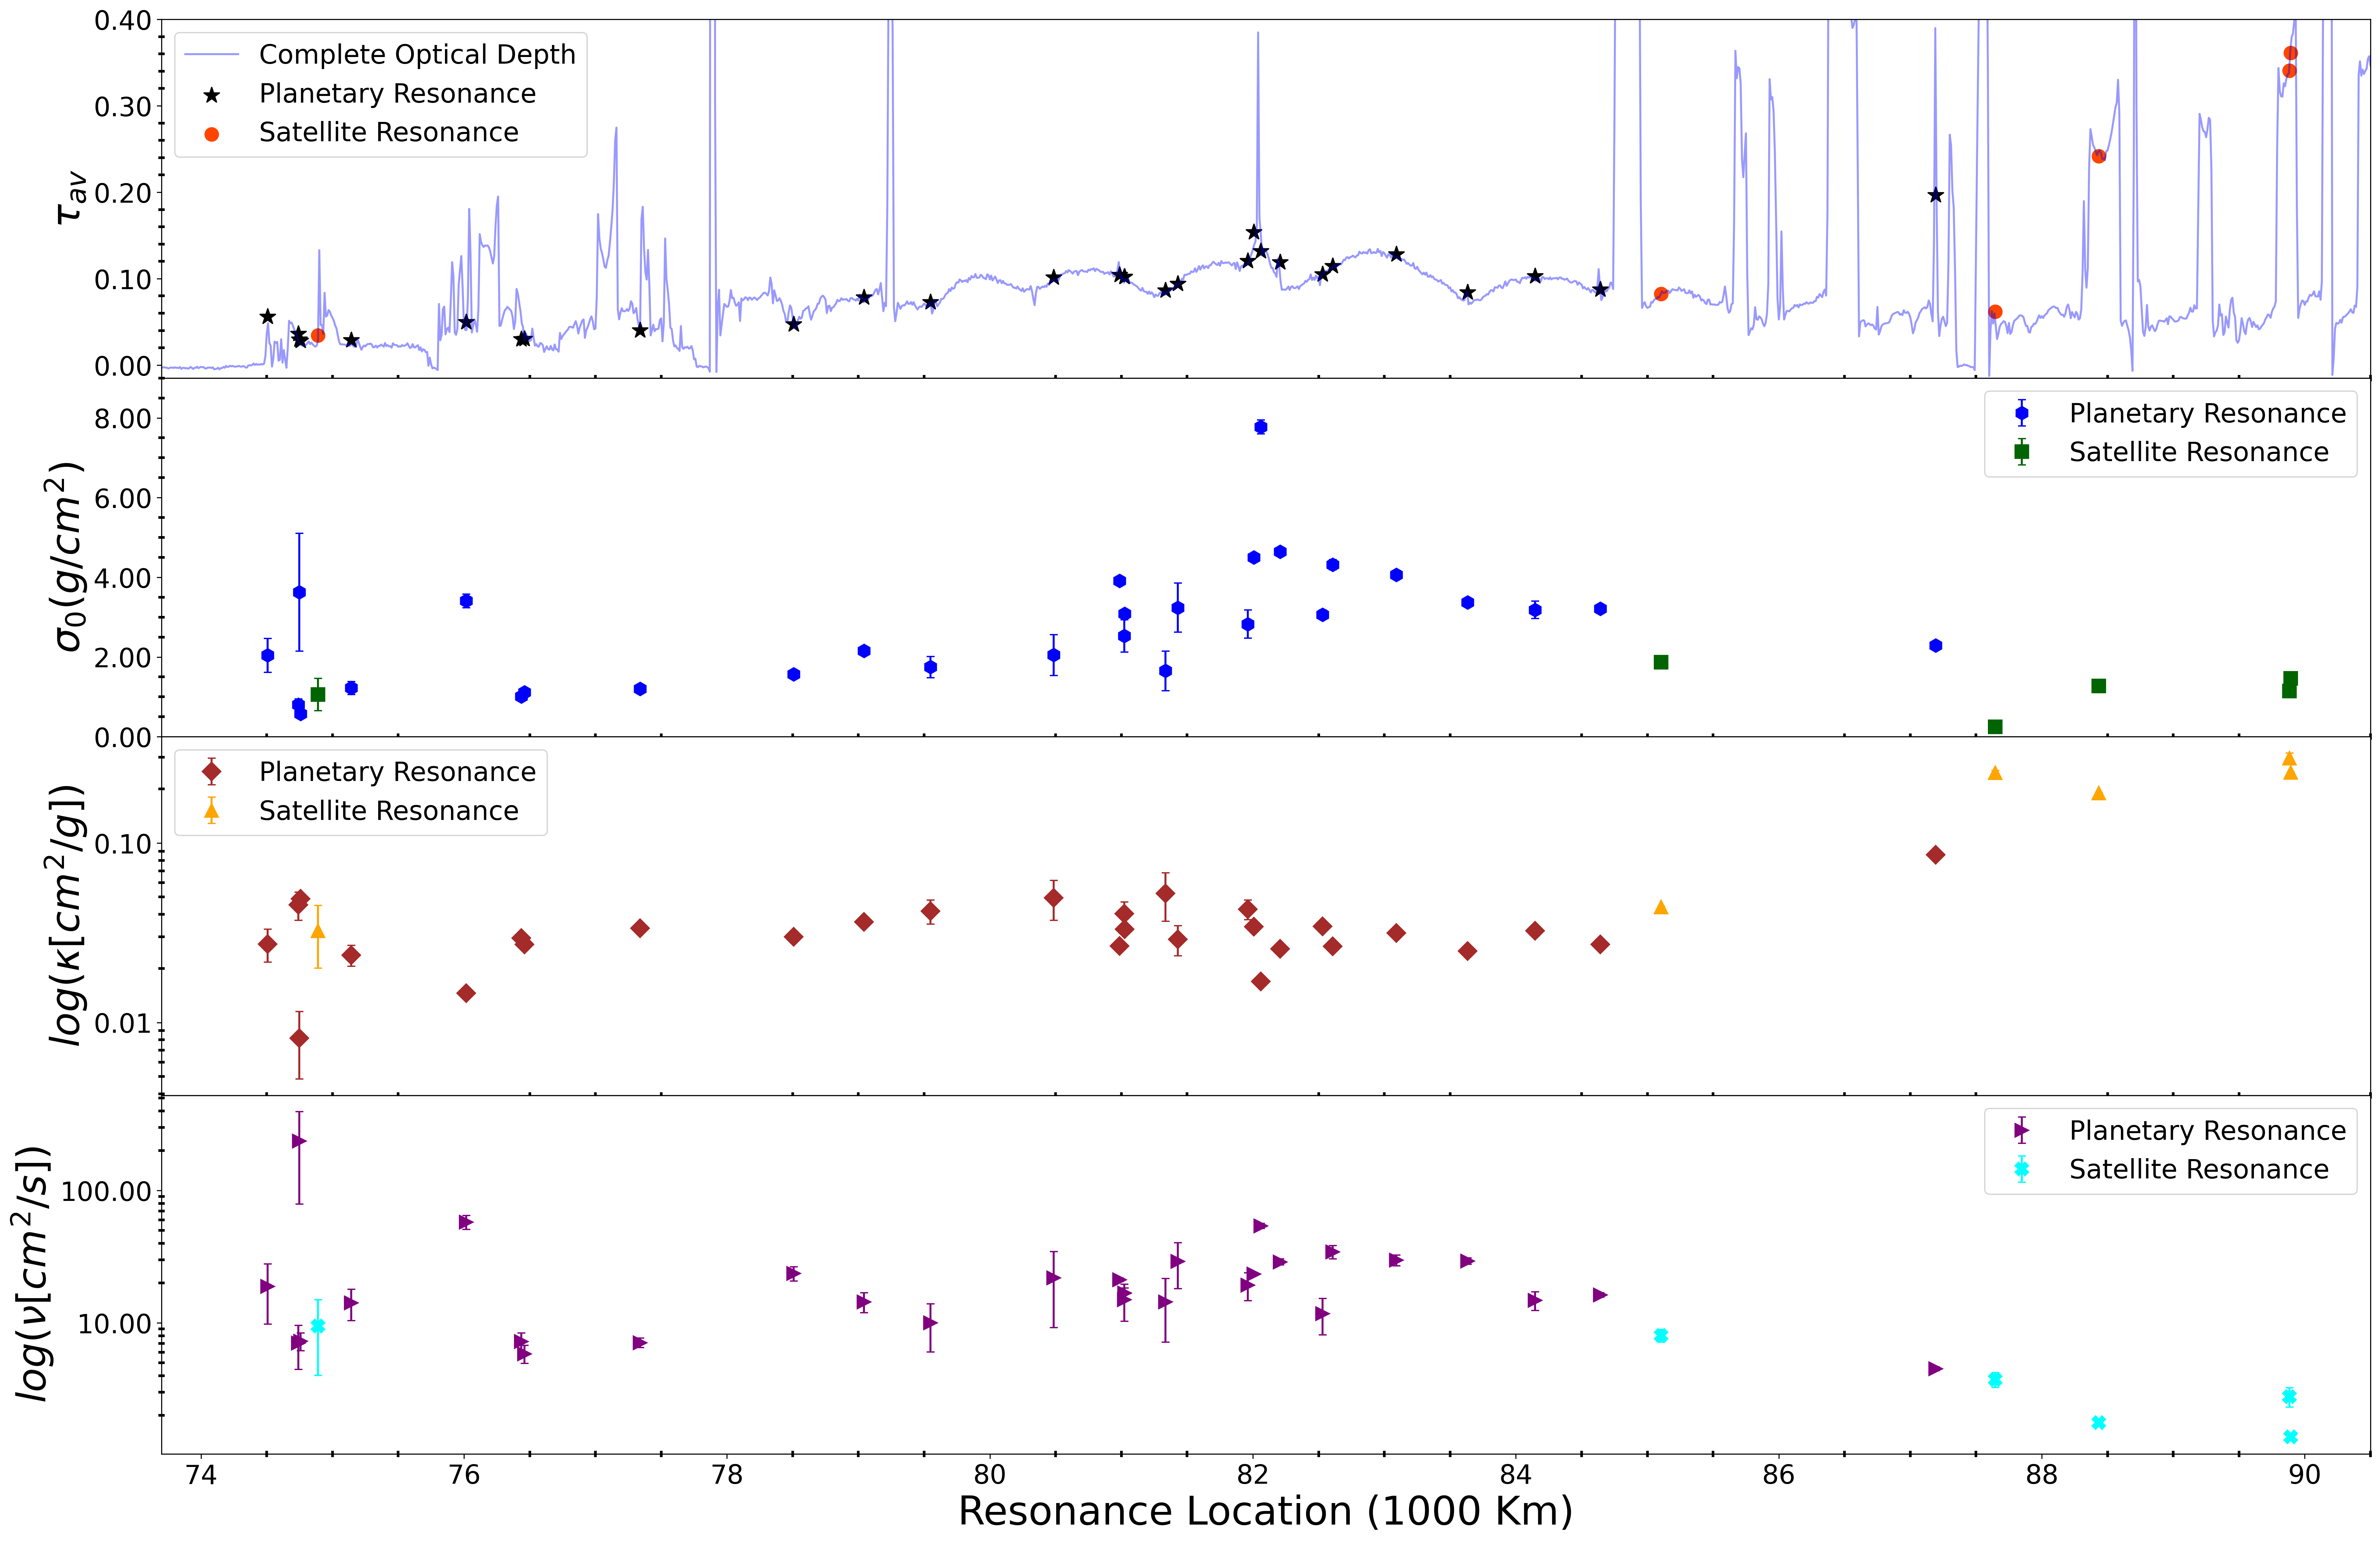
\includegraphics[width=0.9\linewidth]{tau_sigma_kapp_nu_Updated.png}
    \caption{A panel of plots for: Average optical depth, surface mass density mass extinction coefficient and viscosity for satellite and non-Satellite resonances.}
    \label{fig:enter-label}
\end{figure}

%..........................................%....................................%..........

\subsubsection{Model Computation for Saturn's Planetary Normal-mode Amplitudes:}
Figure 17 (a) shows a semi-log plot for the normal-mode amplitude for Saturn, $\mathscr{\bar{A}'}_{l|m|0}$, versus the angular degree $l$, computed using the 29 density wave samples. The colour code $l-|m|$ is proportional to the number of cycles of latitudinal oscillations that take place during Saturn's normal-mode oscillation. The format of such cycle is equivalent to $\sin(\frac{l-|m|+1}{2})$, which shows that there is always a half-cycled oscillation that passes to the equator of the planet for every occurrence of $l-|m|$. From the aforesaid figure, we can see that the normal-mode amplitude is a complex function of the angular degree, as well as $l-|m|$. Again, the figure shows some notable peak amplitudes at $l = 3, 13$ with amplitude values ranging between the set $[10^{-10}, 10^{-9}]$ on the semi-log scale of the plot. Also, we see a notable deep in the trend of result between $l=5$ and $l=8$. A closer look at the result simply shows that between $l=2$ and $l=11$, there are more occurrence of normal-mode oscillations with approximately $l-|m|=0$ cycles with amplitudes ranging between roughly $10^{-11}$ to around $10^{-9}$, except for the two dataset with $l-|m|=2$ that occur within the range of angular degree in description. Also, considering the regions of angular degree $l$ with the set $(11,19]$, we see a trend of result that shows more occurrence of normal-mode oscillations with $l-|m|=4$ compared to those with $l-|m|=2,6,8$. This might suggest there are some form of latitudinal influence on the normal-mode oscillations of Saturn, perhaps latitudinal structures that tend to favour these sorts of pattern we see in the preliminary result. 

On the other hand, figure 17(b) is a semi-log plot for the normal-mode amplitude for Saturn, $\mathscr{\bar{A}'}_{l|m|0}$, versus the oscillation frequency, $\sigma_{lm0}$ computed using the 29 density wave samples. The colour code $l-|m|$ has the same meaning as described previously. The result here shows that, the normal-mode amplitude is also a complex function of the oscillation frequency and also $l-|m|$. Again, the figure shows some notable peak amplitudes between the range $[10^{-10}, 10^{-9}]$ on the log-scale and around $175\mu Hz$ and $475\mu Hz$, and low amplitude of around $10^{-11}$ on a log-scale, between $300\mu Hz$ and $375\mu Hz$. The deep region for this normal-mode frequency spectrum exist between the range of, say, $250\mu Hz$ to around $375\mu Hz$. Normal-modes with $l-|m|=0$ occupy a wider frequency spectrum, between $100\mu Hz$ and $500\mu Hz$, while those modes with $l-|m|=2$ overlap regions with $l-|m|=0$ by occupying between, say,  $375\mu Hz$ and $580\mu Hz$. Also, normal-modes with $l-|m|=4$ occupy the second broadest frequency spectrum (after $l-|m|=0$) within the range of around $440\mu Hz$ to around $650\mu Hz$. Currently we do not have enough data to quantify the trends and spectrum for normal-modes with $l-|m|=6,8$: these are single occurring data points and existing within the range $500\mu Hz$ and $600\mu Hz$. Between  $450\mu Hz$ and $600\mu Hz$, we observed the most overlap in terms of frequency spectrum: normal-mode amplitudes with $l-|m|=0,2,4,6,8$ all coexist within this region, making it complex to attach a defined trend to the frequency spectrum of defined normal-mode oscillations. We can also see that this region is characterized by the most scatter, compared to other regions with little or no scattered data point, hence buttressing our previous statement that the normal-mode amplitude is a complex function of oscillation frequency. 


% DATA TABLE FOR SATURN'S NORMAL-MODE OSCILLATIONS
\begin{table}[h]
\centering
\vspace{-1.5cm} % Adjust the value as needed for vertical spacing before the table
\rotatebox{90}{
%\normal
\begin{tabular}{|c|c|c|c|c|c|c|c|c|c|}  
\hline
\stackon[0pt]{ID}{\stackon[0pt]{Wave}} & \stackon[0pt]{(Km)}{\stackon[0pt]{Range}{Radial}} & \stackon[0pt]{(Km)}{\stackon[0pt]{Location ($r_{L}$)}{Resonance}} & $l$ & $m$ & \stackon[0pt]{(^{o}/day)}{\stackon[0pt]{Speed ($\Omega_{P}$)}{Pattern}} & \stackon[0pt]{$(\mu Hz)$}{\stackon[0pt]{$\sigma_{l|m|0} = |m|\Omega_{P}$}}& \stackon[0pt]{(Unit)}{\stackon[0pt]{$\mathscr{\bar{A}'}_{l|m|0}\times 10^{-10}$}}\\
\hline
$W74.51^{av}$ & 74501.00 - 74509.00 & 74506.900 & 12 & -8 & 1697.339 & 436.556 & 4.188953 $\pm$ 1.625144 \\
W74.74 & 74736.00 - 74743.00 & 74739.850 & 15 & 13 & 1390.843 & 581.303 & 0.468935 $\pm$ 0.151741 \\
W74.75 & 74746.00 - 74748.00 & 74748.300 & 11 & 11 & 1369.932 & 484.476 & 1.000367 $\pm$ 0.716662 \\
W74.76 & 74752.00 - 74762.00 & 74756.600 & 19 & -11 & 1638.389 & 579.416 & 1.128411 $\pm$ 0.096750 \\
W75.14 & 75142.00 - 75144.00 & 75143.000 & 16 & -10 & 1638.983 & 526.933 & 2.150641 $\pm$ 0.511749 \\
W76.02A & 76016.00 - 76018.00 & 76018.100 & 13 & -9 & 1626.530 & 470.636 & 8.496996 $\pm$ 1.322658 \\
W76.44 & 76433.00 - 76436.00 & 76435.400 & 2 & -2 & 2169.260 & 139.483 & 0.349768 $\pm$ 0.060859 \\
$W76.46^{av}$ & 76457.00 - 76462.00 & 76459.500 & 9 & -7 & 1657.720 & 373.070 & 0.448199 $\pm$ 0.088837 \\
W77.34 & 77337.00 - 77339.00 & 77338.900 & 14 & -10 & 1569.078 & 504.459 & 1.246061 $\pm$ 0.140534 \\
W78.51 & 78503.00 - 78509.00 & 78506.750 & 15 & -11 & 1521.410 & 538.047 & 6.120969 $\pm$ 0.702114 \\
W79.04 & 79039.00 - 79045.00 & 79042.300 & 11 & -9 & 1533.336 & 443.671 & 0.855530 $\pm$ 0.136226 \\
W79.55 & 79546.00 - 79550.00 & 79548.920 & 16 & -12 & 1481.152 & 571.428 & 1.823376 $\pm$ 0.748287 \\
W80.49 & 80484.00 - 80488.00 & 80486.100 & 17 & -13 & 1446.654 & 604.629 & 2.371932 $\pm$ 1.070324 \\
W80.99 & 80983.00 - 80989.00 & 80986.150 & 4 & -4 & 1660.363 & 213.523 & 1.086303 $\pm$ 0.028567 \\
W81.023A & 81018.00 - 81030.00 & 81023.100 & 5 & -5 & 1593.630 & 256.176 & 0.191079 $\pm$ 0.055287 \\
W81.024B & 81018.00 - 81030.00 & 81024.150 & 13 & -11 & 1450.495 & 512.968 & 1.607331 $\pm$ 0.086647 \\
W81.33 & 81333.00 - 81336.00 & 81334.275 & 18 & -14 & 1416.734 & 637.672 & 2.134102 $\pm$ 1.025221 \\
W81.43 & 81420.00 - 81430.00 & 81429.550 & 6 & -6 & 1538.237 & 296.726 & 0.122626 $\pm$ 0.045158 \\
W81.96 & 81959.00 - 81965.00 & 81962.450 & 7 & -7 & 1492.457 & 335.877 & 0.194246 $\pm$ 0.041141 \\
W82.01 & 82004.00 - 82009.00 & 82007.750 & 3 & -3 & 1736.645 & 167.499 & 0.810594 $\pm$ 0.012101 \\
W82.06 & 82055.00 - 82065.00 & 82059.400 & 3 & -3 & 1734.999 & 167.341 & 2.941676 $\pm$ 0.115643 \\
W82.21 & 82187.50 - 82207.51 & 82207.500 & 3 & -3 & 1730.293 & 166.887 & 2.125972 $\pm$ 0.068838 \\
W82.53 & 82510.00 - 82530.00 & 82528.750 & 8 & -8 & 1454.224 & 374.026 & 0.095499 $\pm$ 0.025765 \\
W82.61 & 82606.00 - 82608.00 & 82607.750 & 15 & -13 & 1390.843 & 581.303 & 1.722142 $\pm$ 0.241385 \\
W83.09 & 83086.00 - 83096.00 & 83090.650 & 9 & -9 & 1421.844 & 411.411 & 0.597726 $\pm$ 0.023984 \\
W83.63 & 83612.02 - 83637.02 & 83632.020 & 10 & -10 & 1394.056 & 448.189 & 4.438521 $\pm$ 0.190089 \\
W84.15 & 84140.00 - 84150.00 & 84147.100 & 11 & -11 & 1369.910 & 484.469 & 0.279899 $\pm$ 0.043982 \\
W84.64 & 84630.00 - 84650.00 & 84643.200 & 2 & -2 & 1860.752 & 119.646 & 1.349655 $\pm$ 0.042135 \\
W87.19 & 87170.00 - 87210.00 & 87192.800 & 2 & -2 & 1779.548 & 114.425 & 0.293311 $\pm$ 0.011653 \\
\hline
\end{tabular}
\vspace{-1.5cm}
}
\caption{Data table for Saturn's Normal-mode Amplitudes and corresponding oscillation frequencies for each non-Satellite resonances.}
\end{table}

% PLOTS FOR NORMAL-MODE OSCILLATIONS FOR SATURN

\begin{figure}[htbp]
    \centering
    \begin{subfigure}[b]{0.5\linewidth}
        \centering
        \includegraphics[width=\linewidth]{updated_NORMALMODEAMPLITUDE.png}
        \caption{}
        \label{fig:amplitude_vs_degree}
    \end{subfigure}
    \hspace{0.5cm}
    \begin{subfigure}[b]{0.5\linewidth}
        \centering
        \includegraphics[width=\linewidth]{amplitude_PLUS_frequency.png}
        \caption{}
        \label{fig:amplitude_vs_frequency}
    \end{subfigure}
    \hspace{0.5cm}
    \begin{subfigure}[b]{0.5\linewidth}
        \centering
        \includegraphics[width=\linewidth]{mormalmode_RATIOMAIN.png}
        \caption{}
        \label{fig:normal_mode_RATIOPLOT}
    \end{subfigure}
    \caption{A semi-log plot for Saturn's normal-mode amplitude. (a) Versus angular degree. (b) Versus oscillation frequency. (c) Versus mode energy mid-point radii.}
    \label{fig:saturn_normal_mode_amplitude}
\end{figure}



%.................................................................................
\section{Discussions}

More preliminary results regarding normal-mode amplitude computations is shown in figure 17(c), a semi-log plot of normal-mode amplitude versus mode energy mid-point radii estimated with respect to Saturn's equatorial radius($R_{eq}$ = 60,268 Km). The horizontal axis could also be referred to as the depth of the planet, with the origin (center) being the $0.0$ point, while the surface being the $1.0$ point. Trends from this plot show that there might be two classes of normal-mode excitation within Saturn: the deep modes and shallow modes of excitation. Normal-modes with $l = 2,3,4$ could be attributable to sources of excitation deep within the planet's interior, while modes with $l>4$ could be associated with excitation sources at regions close to the surface of the planet.

A similar version of the aforesaid plot is show in the figure 18(a, b). Figure 18(a) shows the simulated mode energy mid-point radii associated with the average energy for the normal-mode amplitude, versus the corresponding angular degree. It shows the mode energy midpoint locations, up to $|m|=14$ and $\ell-|m|=0,2,4,6,8$. The results from this simulation clearly shows that there is a somewhat exponential increase in mode energy mid-point radii with respect to an increase in angular degree. Normal-mode oscillations with lower angular degrees tend to occur at regions close to the center of the planet, while normal-mode oscillations with relatively higher angular degrees are located at regions close to the surface of the planet.

Besides, figure 18(b) shows a metric for mode depth from a simulated Saturn models involving the energy associated with each mode. Looking at $\rho |\vec v|^{2}$, the $\vec v$ is the mode velocity perturbation vector and $\rho$ is just the background density of the planet, which amounts to a kinetic energy density of the mode involved. Integrating this over the volume of the planet simply gives the mode energy for the corresponding normal-mode oscillation. We ascribed a depth to each mode by asking at what radius this mode energy integral reaches half its total value. To arrive at the result shown, we weight the integrand by $r^{2}$ from the volume element. Each mode in the plot has a dot showing the integral's midpoint location. Our observations show that the modes at $\ell=|m|=2,3,4,5$ all have considerable amplitude in the g-mode cavity, which might imply that they all have peak average mode energies at regions close to the center of the planet, while the modes with $\ell > 5$ all have peak average energies at regions close to the surface of the planet, which might mean that there are potentially deep sources and shallow sources of planetary normal-mode excitation for Saturn.

\begin{figure}
    \centering
    \begin{subfigure}{0.6\linewidth}
        \centering
        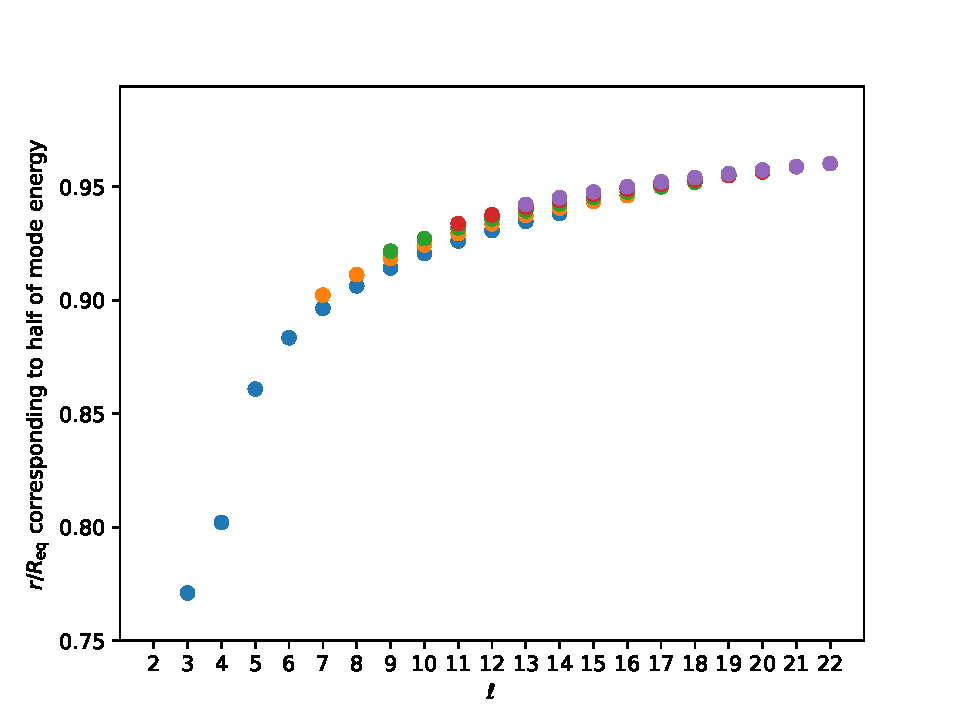
\includegraphics[width=\linewidth]{mode_energy_midpoint_radii.pdf}
        \caption{Simulated mode energy mid-point radii(for average mode energy) versus angular degree.}
        \label{fig:sub1}
    \end{subfigure}
    \hspace{-5.5cm} % Adjust the horizontal spacing here
    \begin{subfigure}{1.14\linewidth}
        \centering
        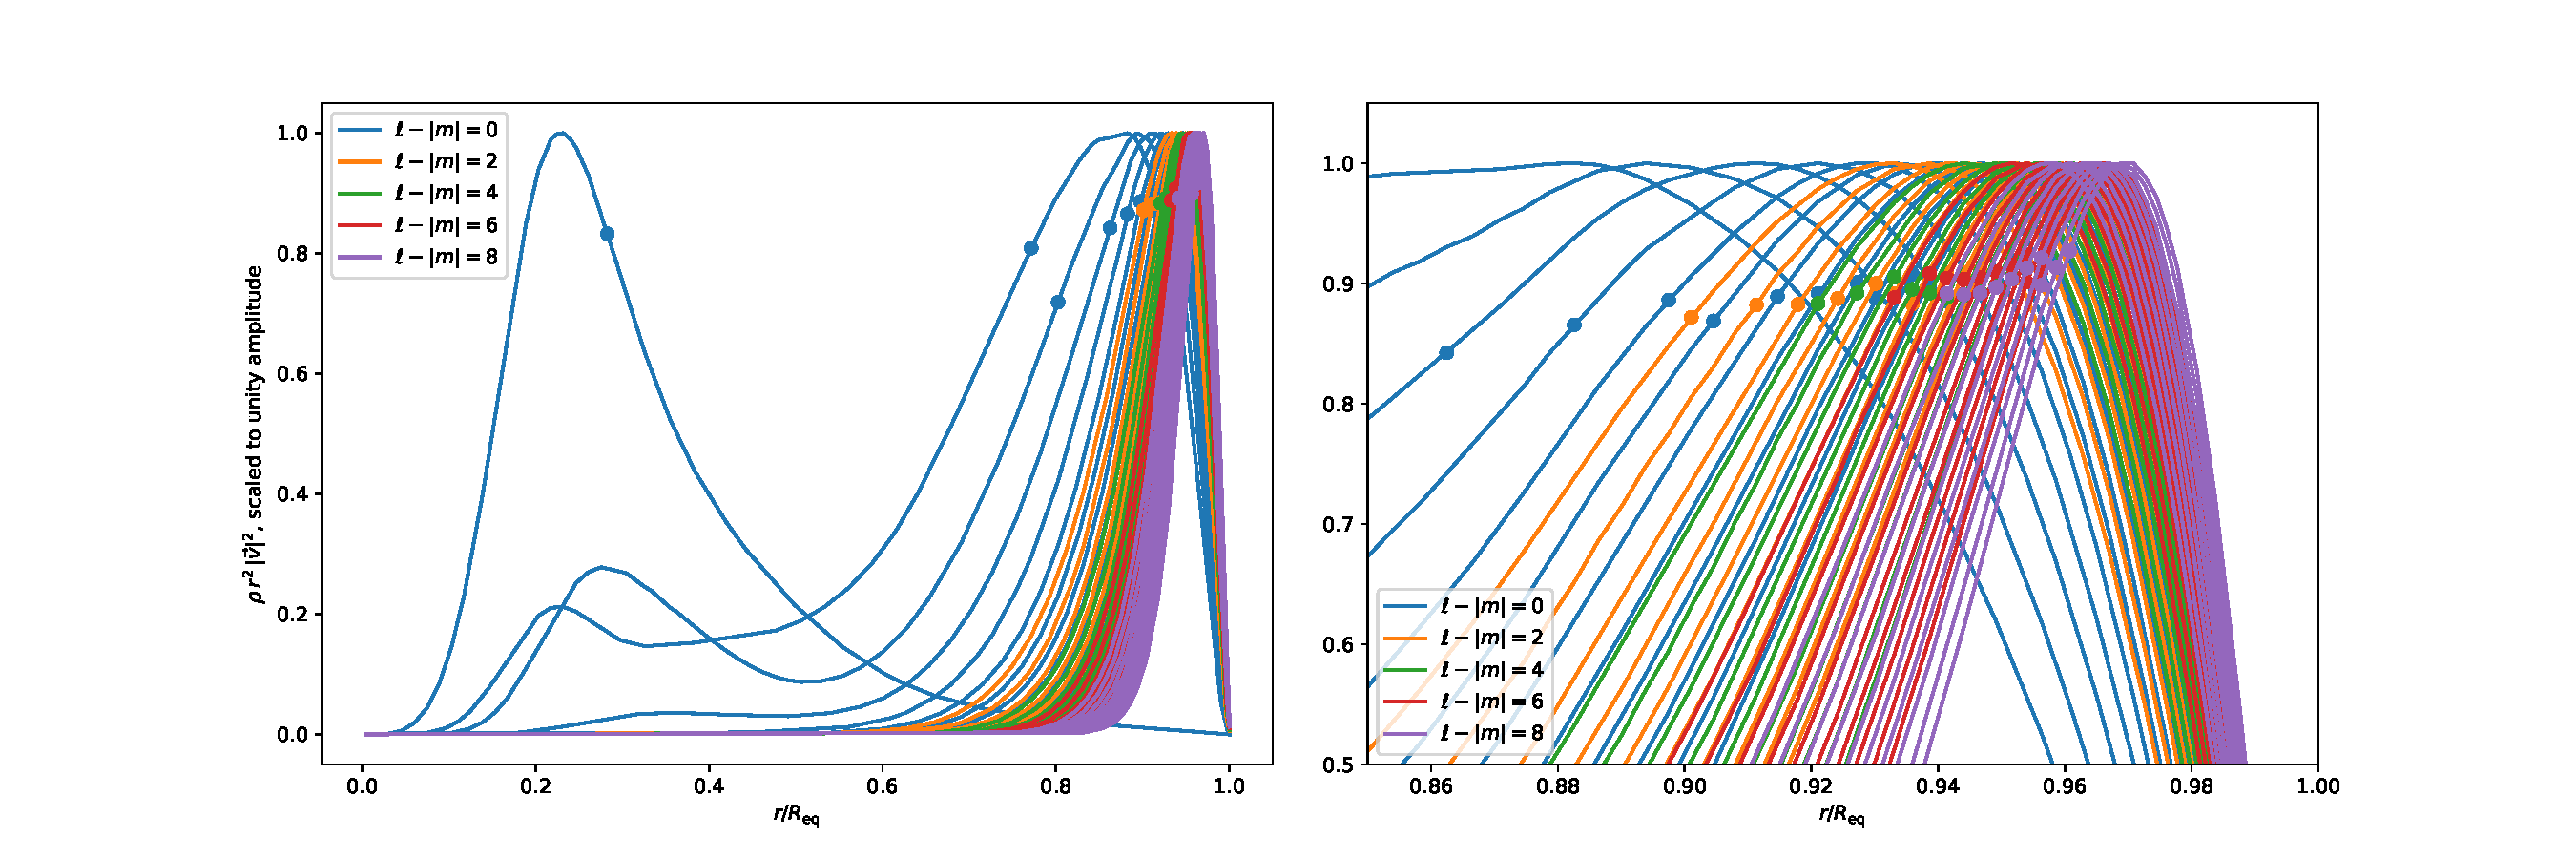
\includegraphics[width=\linewidth]{mode_energy_integrands (2).pdf}
        \caption{Simulated mode energy versus mode energy mid-point radii.}
        \label{fig:sub2}
    \end{subfigure}
    \caption{Plots for simulations involving: (a) Mode energy mid-point radii versus angular degree.  (b) Mode energy versus mode energy mid-point radii.}
    \label{fig:overall}
\end{figure}

%.................................................................................

\section{Future Directions}
There is still much to learn about spiral density waves in Saturn's rings, and efficient algorithms for Fourier transforms are an important tool for their analysis. One promising direction for future research is the use of Fourier transforms to study the interaction between spiral waves and other phenomena in the rings, such as resonances with nearby moons. Additionally, new data from the Cassini spacecraft and future missions to Saturn could provide even more detailed information about the structure and dynamics of the rings, opening up new avenues for analysis. To help achieve these objectives, we plan to achieve a more efficient correction factor for our customized algorithm, to help produce efficient and effective results during usage. 




\textbf{Beyond the Table: Considerations and Open Questions}

While the model computations provide valuable insights, it is crucial to acknowledge potential limitations and open questions:

Model simplifications: The model might not incorporate all the complex gravitational and collisional interactions in play within the rings, leading to potential discrepancies with real-world observations.
Uncertainty estimates: The reported uncertainties in both $\sigma_{0}$ and $\kappa$ highlight the need for further refinement of the model and additional observational data to improve accuracy.
Temporal variations: The model might not capture the dynamic nature of the rings, where particle distribution and properties might change over time due to collisions, interactions with moons, and external forces.

These limitations and open questions underline the importance of ongoing research efforts:

Refining the model: Incorporating additional factors like non-axisymmetric gravitational perturbations and collisional processes could enhance the model's accuracy and predictive power.
Combining models and observations: Utilizing a multi-pronged approach that combines data from various missions, telescopes, and theoretical models can provide a more comprehensive understanding of ring dynamics.
Investigating temporal variations: Monitoring the rings over time through long-term observations can reveal insights into how their structure and properties evolve due to various celestial interactions.

By addressing these limitations and pursuing further research, we can solidify our understanding of the intricate dance between Saturn's moons, its captivating rings, and the dynamic forces shaping this awe-inspiring planetary system.







\section{Conclusion}

Satellite Resonances: The results suggests that different moons of Saturn trigger distinct density wave patterns with varying degrees of damping and viscosity. This information is crucial for understanding the dynamics of Saturn's rings and the interactions between the planet and its moons.

In conclusion, our study has shed new light on the behavior of waves within Saturn's rings and the factors that influence them. By using efficient Fourier transform algorithms, we were able to quantify the impact of the planet's internal structure on the behavior of these waves. As we continue to uncover new information about Saturn and its rings, these findings will serve as a critical foundation for future research efforts aimed at further exploring the mysteries of our solar system.

\section{Data Availability Statement}
The corresponding authors are committed to promoting open and transparent research practices. They are willing to share the data, models, or codes to facilitate further analysis and validation of the research findings. Collaborators, fellow researchers, and interested parties are encouraged to reach out to the corresponding authors to obtain the requested information. It is important to note that the availability of the data, models, or codes is subject to any applicable legal, ethical, or privacy restrictions. The corresponding authors will ensure that any shared materials comply with relevant regulations and guidelines to protect the privacy and confidentiality of participants or sensitive information. Additionally, the corresponding authors may provide supplementary materials or documentation to enhance the understanding and reproducibility of the research. These additional resources can assist readers in replicating the study or building upon its findings. The corresponding authors can be contacted via their provided contact details or through the designated communication channels outlined in the research publication. They will endeavor to respond to requests in a timely manner, keeping in mind the complexity and scope of the information being requested. Overall, the corresponding authors are dedicated to fostering a culture of collaboration and knowledge sharing, aiming to contribute to the advancement of scientific inquiry and progress.

\section{Acknowledgements}
I gratefully acknowledge the Maker of the Universe, for unending inspiration and momentum to continue in times of greatest need. I also appreciate Prof. Matthew Hedman and other esteemed co-authors for helpful comments, suggestions and contributions. This research has made use of data obtained from the recent Cassini Mission (2004-2017), as well as softwares from Python libraries. 


\section{Appendix}
\label{sec:appendix}


\subsection{Code Snippets For Density Wave Analysis}
\label{subsec:code}

\begin{lstlisting}[language=Python, caption=Python code snippet for Spiral Density Wave Analysis.]
# Import all the required libraries 
import numpy as np
import scipy as sp
import matplotlib.pyplot as plt
from scipy.io import readsav
from scipy import signal as signal

# Set Parameters for the specific wave.
   
    # datfile = idl save file of the profiles
    # m = (signed) azimuthal wavenumber of wave
    # omp = Nominal Wave pattern speed in degrees/day
    # omr = Range of pattern speeds to consider in degrees/dat
    # xr = Range of radii to plot and compute wavelets (in 1000 km)
    # rback = Radius range of blank region for identifying good profiles (in km)
    # rwave = Radius range  containing the wave (in km)
    # wrange(frange) = Range of spatial wavelegths(frequencies) to compute in the wavelet
    # mthres = Threshold deviation for normal optical depth in range rback
    # rthres = Maximum allowed resolution in range rwave
    # rangedisp = range of signals shown in power wavelets
    # badoccnames = Names of occultations to be removed that look problematic on visual inspection

datfile = '...'
m = ...
omp = ...
omr = ...
xr=  [...]
rback = [...]
rwave = [...] 
wrange = [...]
mthres = ...
rthres = ...
rangedisp = ...

badoccnames = ["...","..."] # Either one or more occultations could be bad.

# Read the data file into python
data = readsav(datfile)
radi = data.radi
lons = data.lon
times = data.etime
resrs = data.res
dat = np.transpose(data.dat)
radi = np.array(radi)
dat = np.array(dat)
lons = np.array(np.transpose(lons))
times = np.array(np.transpose(times))
resrs = np.array(np.transpose(resrs))

nf = len(data.labs)
nr = len(radi)

# Convert to Normal Optical Depth
dat[dat<1e-10] = 1e-10 #Removes negative signals to avoid numerical errors for log transform
tau = -np.log(dat)
for i in range(nf):
    tau[i] = tau[i]*np.abs(np.sin(data.b[i]*3.14159/180.))

# yr is year of observation after 2000    
yr = times[0:nf,0]/24/3600/365.25

# Determine average optical depth and maximum resolution in regions
taum = np.mean(tau[0:nf,(radi > rwave[0]) &(radi < rwave[1])], axis=1)
rmax = np.max(resrs[0:nf,(radi > rwave[0]) &(radi < rwave[1])], axis=1)

mtaum = np.median(taum)

# Select profiles with reasonable optical depths and resolution, also can include cut on times here
taux = tau[(np.abs(taum-mtaum) < mthres) & (rmax<rthres) & (yr < 18),0:nr]
lonx = lons[(np.abs(taum-mtaum)<mthres) & (rmax<rthres) & (yr < 18),0:nr]
timex = times[(np.abs(taum-mtaum)<mthres)& (rmax<rthres) & (yr < 18),0:nr]
labx = data.labs[(np.abs(taum-mtaum)<mthres)& (rmax<rthres) & (yr < 18)]
nfx = len(taux)
print(nfx)

# Plot the profiles for visual inspection
print('Automatically Selected Profiles')

plt.figure(figsize=(6,30))
for i in range(0,len(taux)):
    plt.plot(radi/1e3,taux[i]+i)
    plt.text(xr[1],i,labx[i])
plt.xlim(xr)
plt.xlabel('Radius (1000 km)')
plt.ylabel('Normal Optical Depth + offset')
plt.show()

# Remove occs flagged as bad by visual inspection
badoccs = np.zeros(nfx)
for i in range(0,len(badoccnames)):
    for j in range(0,nfx):
        occname=str(labx[j])
        if badoccnames[i] in occname:
                badoccs[j]=1

taux = taux[(badoccs == 0),0:nr]
lonx = lonx[(badoccs == 0),0:nr]
timex = timex[(badoccs == 0),0:nr]
labx = labx[(badoccs == 0)]
nfx = len(taux)
                      
# Plot the profiles for visual inspection after removing named occs
print('After Excluding Profiles by hand')
plt.figure(figsize=(6,30))
for i in range(0,len(taux)):
    plt.plot(radi/1e3,taux[i]+0.14*i)
    plt.text(xr[1],0.14*i,labx[i])
plt.xlim(xr)
plt.xlabel('Radius (1000 km)')
plt.ylabel('Normal Optical Depth + offset')
plt.show()

# Select out the parts of the profiles shown (speeds up wavelet transforms)
taux = taux[0:nfx,(radi>xr[0]*1e3) & (radi<xr[1]*1e3)]
lonx = lonx[0:nfx,(radi>xr[0]*1e3) & (radi<xr[1]*1e3)]
timex = timex[0:nfx,(radi>xr[0]*1e3) & (radi<xr[1]*1e3)]
radix = radi[(radi>xr[0]*1e3) & (radi<xr[1]*1e3)]
nrx = len(radix)

# Codes for Continous Wavelet Transform (and Parameters)
def waveletls(x, y, lambdas, param, wave=None):
    # nx is the number of elements in x
    nx = len(x)
    # nl is the number of elements in lambdas
    nl = len(lambdas)
    # fy is the Fourier Transform of y. We still need to import the fft module for this step.
    fy = np.fft.fft(y)
    # dx is the difference between the first and second elements of x
    dx = x[1] - x[0]
    # k is an array of evenly spaced values between 0 and nx
    k = np.arange(nx)
    # omegak is the frequency of each value in k
    omegak = 2*np.pi*k/nx/dx
    # q is a boolean array of the values in k greater than nx/2
    q = np.where(k > nx/2)
    # For elements in omegak where the corresponding value in k is greater than nx/2,
    # The value of omegak is set to 0 minus the frequency of the corresponding value in k
    omegak[q] = 0 - 2*np.pi*k[q]/nx/dx
    # omegakx is a matrix where each row is a copy of omegak
    omegakx = np.outer(omegak, np.ones(nl))
    # scales is the result of multiplying lambdas by a constant term
    scales = (param + np.sqrt(param**2 + 2))*(lambdas)/4/np.pi
    # scalex is a matrix where each column is a copy of scales
    scalex = np.outer(np.ones(nx), scales)
    
    scalex = scalex.astype(float) # This line of code was added to boycott the issues with the lambdas parameter
    
    # morlet is the wavelet transform of fy and lambdas
    morlet = 1/np.pi**.25*np.exp(-(scalex*omegakx - param)**2/2.0)
    # wave is a complex matrix with dimensions nx by nl
    if wave is None:
        wave = np.empty((nx, nl), dtype=complex) # Changed positions of nx and nl 2/14/2023
    # for each row of morlet, wave is set to the inverse Fourier Transform of the product of fy and the row
    for i in range(nl):
        wave[:,i] = np.fft.ifft(fy*morlet[:,i], axis=-1)
    # return the final computed wavelet matrix
    return wave, morlet

# Link Continous Wavelet Transforms to signal properties
nw = len(radix)
param = 6.
lambdas = np.linspace(wrange[0], wrange[1], nw, retstep=True)[0]
x = radix
scales = (param + np.sqrt(param**2 + 2))*(lambdas)/4/np.pi
cwtmatmat = np.zeros([nfx,nrx,nw], dtype=complex)

# Implementation of Continous wavelet transforms to signal data
for i in range(0,nfx):
        print(i,labx[i])
        cwtmatmat[i,0:nrx,0:nw], morlet = waveletls(x, taux[i,0:nrx], lambdas, param, wave=None)
        plt.imshow((np.abs(cwtmatmat[i,0:nrx,0:nw])),
             vmin=0, vmax=rangedisp, origin='lower', extent=[wrange[0],wrange[1],xr[0],xr[1]], aspect='auto')
        plt.xlabel('Spatial Wavelength (km)')
        plt.ylabel('Radius (1000 km)')
        plt.show()

# Compute the phases for the nominal pattern speed
et0 = 10.0*365.25*24*3600   # Epoch of ten (10) years
npat = 20 # Must be even
phases = np.zeros([nfx,nrx])
phases[0:nfx,0:nrx] = np.abs(m)*(lonx-(omp)/24/3600*(timex-et0))
print(np.min(phases), np.max(phases))
phases = ((phases % 360.)+360.)%360.
print(np.min(phases), np.max(phases))
cp = np.cos(phases*np.pi/180)
sp = np.sin(phases*np.pi/180)

# Apply phase shifts to the wavelet transform
# Also plots Power of the Average phase corrected wavelet for visual inspection
cwaver = np.real(cwtmatmat)
cwavei = np.imag(cwtmatmat)
cwavex = np.zeros([nfx,nw,nrx])
cwavey = np.zeros([nfx,nw,nrx])
for i in range(0,nw):
    cwavex[0:nfx,i,0:nrx] = cwaver[0:nfx,i,0:nrx]*cp[0:nfx,0:nrx]+cwavei[0:nfx,i,0:nrx]*sp[0:nfx,0:nrx]
    cwavey[0:nfx,i,0:nrx] = cwavei[0:nfx,i,0:nrx]*cp[0:nfx,0:nrx]-cwaver[0:nfx,i,0:nrx]*sp[0:nfx,0:nrx]

# Compute average phase corrected wavelets for each pattern speed 
cwaverc = np.mean(cwavex, axis=0)
cwaveic = np.mean(cwavey, axis=0)

# Compute average wavelet power, power of average phase-corrected wavelet for nominal case, and power ratio and make plots of all of them
cwavea = np.mean(np.sqrt(cwavex**2+cwavey**2), axis=0)
cwavez = np.sqrt(cwaverc**2+cwaveic**2)
cwavezz = np.zeros([npat,nw,nrx])
cwavezz = cwavez/cwavea

print('Average Wavelet Power')
plt.imshow(cwavea,
           vmin=0, vmax=rangedisp, origin='lower', extent=[wrange[0],wrange[1],xr[0],xr[1]], aspect='auto')
plt.xlabel('Spatial Wavelength (1/km)') 
plt.ylabel('Radius (1000 km)')
plt.show()

print('Power of Average PCW')
plt.imshow(cwavez,
           vmin=0, vmax=rangedisp, origin='lower', extent=[wrange[0],wrange[1],xr[0],xr[1]], aspect='auto')
plt.xlabel('Spatial Wavelength (1/km)')
plt.ylabel('Radius (1000 km)')
plt.show()

print('Power Ratio')
plt.imshow(cwavezz,
           vmin=0, vmax=rangedisp+1, origin='lower', extent=[wrange[0],wrange[1],xr[0],xr[1]], aspect='auto')
plt.xlabel('Spatial Wavelength (1/km)')
plt.ylabel('Radius (1000 km)')
plt.show()

# Continous Wavelet Transform Reconstruction
scales = (param + np.sqrt(param**2 + 2))*(lambdas)/4/np.pi
widths = scales
widthx = np.zeros([nrx,nw])
for i in range(0,nrx):
        widthx[i,0:nw]=widths
#for i in range(0,nw):
cwaverec = 6*(wrange[1]-wrange[0])*np.mean(np.real(cwaverc)/((widthx)), axis=1)
cwaverec2 = 6*(wrange[1]-wrange[0])*np.mean(np.real(cwaveic)/((widthx)), axis=1)
profrec=cwaverec
profrec2=cwaverec2
taub=np.median(taux, axis=0) 
# Or use t_av = np.mean(tau_av) where necessary: tau_av = taub[(radix>rwave[0]) & (radix<rwave[1])]
nprofrec = profrec/taub

# Plot all three quantities
plt.figure(figsize=(19,9))
print('Reconstructed Profile')
plt.plot(radix/1e3,profrec)
plt.xlim(xr)
plt.xlabel('Radius (1000 km)')
plt.ylabel('Normal Optical Depth')
plt.show()

plt.figure(figsize=(19,9))
print('Average Background Profile')
plt.plot(radix/1e3,taub)
plt.xlim(xr)
plt.xlabel('Radius (1000 km)')
plt.ylabel('Normal Optical Depth')
plt.show()

plt.figure(figsize=(19,9))
print('Reconstructed Profile (Normalized to background Optical Depth)')
plt.plot(radix/1e3,nprofrec)
plt.xlim(xr)
plt.xlabel('Radius (1000 km)')
plt.ylabel('Normal Optical Depth')
plt.show()

# Codes For Wave-fitting Routine

# Linear Density Wave Equation for the Spiral Wave, as given in the PDF document attached
def wavefunc(x,a,xd,phi0,xr,xf):
     return (a/xf)*((x - xr)/1)*np.exp(-(np.abs((x - xr)/xf))**3/xd**3)*np.cos(
           phi0-(((x - xr))**2/xf ** 2)-(3*np.pi / 4))*(1+np.sign(m)*np.sign((x-xr)/xf))

# Import the curve_fit routine from Scipy
from scipy.optimize import curve_fit

# We run the code to fit the parameters in wavefunc to prof versus radi.
# Best-fit values are output as fit
# It returns covar, which are the covariances in the fit parameters
# Bounds forces a to be between 0 to 0.1, 
# xd to be between 1 and 40,
# phi0 to be between 0 and 2pi, 
# xr to be between -10 and 10 and 
# xf to be between 0.5 and 4
# Note that these ranges may not work for all waves, they may vary in some cases.

# Define the radial offset
radaf = radix - $r_{L}$ # The resonant radius is different for each wave.

fit, covar=curve_fit(wavefunc,radaf,nprofrec, bounds= ([...]), method='trf')

# Print the fit parameters
print('Fit Parameters nprofrec')
print('Amplitude',fit[0])
print('Damping Length',fit[1])
print('Initial Phase',fit[2])
print('Resonance Offset',fit[3])
print('Winding Parameter',fit[4])

# Compute the model profile given the fit parameters.
mod2=wavefunc(radaf,fit[0],fit[1],fit[2],fit[3],fit[4])

# Remote sensing data (in blue) and the fit model (in orange)
plt.figure(figsize=(19,9))
plt.xlabel('Radius (km)')
plt.ylabel('Spiral Density Wave Signal')
plt.plot(radaf,nprofrec)
plt.plot(radaf,mod2)
plt.xlim([...])
plt.ylim([...])
plt.title("...")
\end{lstlisting}



\subsection{Additional Analysis For Satellite and Planetary Resonances}


\paragraph{List of Faulty Occultations Excluded: Satellite and Planetary Resonances}

\begin{table}
\centering
\vspace{-1.5cm}
%\vspace{0.01pt} % Adjust the value as needed
\rotatebox{90}{
\normal
%\begin{tabular}{lllll}
\begin{tabular}{|c|c|c|c|c|c|c|c|c|c|}
\hline
\stackon[0pt]{Name}{\stackon[0pt]{Resonance}} & \stackon[0pt]{(Km)}{\stackon[0pt]{Range}{Radial}} & \stackon[0pt]{(Km)}{\stackon[0pt]{Location}{Resonance}} & $l$ & $m$ & Faulty Occultations \\
\hline
\stackon[0pt]{Resonance}{\stackon[0pt]{Satellite}} & \saturn & \saturn & \saturn & \saturn & \saturn \\
\hline
Mimas 4:1 & 74880.00 - 74895.00 &  74890.07 & - & 2 & ["RLyr202e","RCas194e"] \\
Pan 2:1 & 85090.00 - 85130.00 & 85105.02 & - & 2 & ["L2Pup206e","betPeg108i","betPeg172i","L2Pup201i","RCas191i",  "muCep191i","RSCnc085e","RCas106i"] \\
Atlas 2:1 & 87640.00 - 87650.00 & 87645.68 & - & 2 & ["muCep191i","gamCru094i","RLyr200i"] \\
Prometheus 4:2 & 88420.00 - 88440.00 & 88434.12 & - & 3 & ["alpSco245i","RCas106i","VYCMa269i"] \\
Mimas 6:2 & 89870.00 - 89890.00 & 89884.00 & - & 3 & ["RCas243i","L2Pup199e","RCar191i","betPeg170e","gamCru079i","gamCru073i"] \\
Pandora 4:2 & 89887.00 - 89897.00 & 89893.68 & - & 3 & ["gamCru291i","RCas243i","L2Pup199e","RCar191i","gamCru079i","gamCru073i"] \\
\hline
\stackon[0pt]{Resonance}{\stackon[0pt]{Planetary}} & \saturn & \saturn & \saturn & \saturn & \saturn \\
\hline
$W74.51^{av}$ & 74501.00 - 74509.00 & 74506.90 & 12 & -8 & ["RCas243i","gamCru094i","RCas194e","RCas191i","RLyr199i"] \\
W74.74 & 74736.00 - 74743.00 & 74739.85 & 15 & 13 & ["RLyr199i","gamCru291i","gamCru089i","RCas191i","alpAur041i","RCas243i"] \\
W74.75 & 74746.00 - 74748.00 & 74748.30 & 11 & 11 & ["RLyr199i","gamCru291i","alpAur041i","RCas243i","RCas191i","RCas185i"] \\
W74.76 & 74752.00 - 74762.00 & 74756.60 & 19 & -11 & ["RLyr199i","alpAur041i","RCas243i"]\\
W75.14 & 75142.00 - 75144.00 & 75143.00 & 16 & -10 & ["alpAur041i","RLyr208e","RLyr202e","L2Pup206e","L2Pup201i","muCep191i","muCep185e"] \\
W76.02A & 76016.00 - 76018.00 & 76018.10 & 13 & -9 & ["RCas243i","lamVel268i"]\\
W76.44 & 76433.00 - 76436.00 & 76435.40 & 2 & -2 & ["gamCru255i","gamCru268i","gamCru100i","RLyr198i"] \\
$W76.46^{av}$ & 76457.00 - 76462.00 & 76459.50 & 9 & -7 &  ["gamCru255i","RLyr198i","muCep193i","muCep191i","gamCru100i"] \\
W77.34 & 77337.00 - 77339.00 & 77338.900 & 14 & -10 & ["muCep191i","2Cen194e","lamVel173i"] \\
W78.51 & 78503.00 - 78509.00 & 78506.750 & 15 & -11 & ["gamCru187e","RCar191i","gamCru276i","alpAur041i"]\\
W79.04 & 79039.00 - 79045.00 & 79042.300 & 11 & -9 & ["L2Pup205e","RCas185i","RCas191i","alpSco115i"]\\
W79.55 & 79546.00 - 79550.00 & 79548.920 & 16 & -12 & ["alpAur041i","gamCru264i","gamCru255i"]\\
W80.49 & 80484.00 - 80488.00 & 80486.100 & 17 & -13 & ["RCas185i","muCep185e"]\\
W80.99 & 80983.00 - 80989.00 & 80986.150 & 4 & -4 & ["gamCru268i","L2Pup205e"]\\
W81.023A & 81018.00 - 81030.00 & 81023.100 & 5 & -5 & ["RCas185i","RLyr202e"]\\
W81.024B & 81018.00 - 81030.00 & 81024.150 & 13 & -11 & ["RLyr202e","RCas185i"]\\
W81.33 & 81333.00 - 81336.00 & 81334.275 & 18 & -14 & ["gamCru269i"]\\
W81.43 & 81420.00 - 81430.00 & 81429.550 & 6 & -6 & ["L2Pup201i","RCas185i","RHya036i","RSCnc080e","WHya180i"]\\
W81.96 & 81959.00 - 81965.00 & 81962.450 & 7 & -7 & ["RCas185i","RCar191i"]\\
W82.01 & 82004.00 - 82009.00 & 82007.750 & 3 & -3 & ["VYCMa269i","RCas194e","L2Pup201i","RCar191i","WHya186e"]\\
W82.06 & 82055.00 - 82065.00 & 82059.400 & 3 & -3 & ["VYCMa269i","RCas243i","RCas194e","L2Pup201i","RCar191i"]\\
W82.21 & 82187.50 - 82207.51 & 82207.500 & 3 & -3 & ["alpAur041i","RCas106i","RCas185i","muCep185e","muCep193i","L2Pup201i","L2Pup206e","RCas243i"]\\
W82.53 & 82510.00 - 82530.00 & 82528.750 & 8 & -8 & ["RCas185i","gamCru089i","gamCru081i","gamCru094i"]\\
W82.61 & 82606.00 - 82608.00 & 82607.750 & 15 & -13 & ["RLyr200i","RSCnc080e","muCep191i","muCep193i","RCas185i"]\\
W83.09 & 83086.00 - 83096.00 & 83090.650 & 9 & -9 & ["RCar191i","RSCnc080i","RSCnc085i","muCep191i","RLyr199i"]\\
W83.63 & 83612.02 - 83637.02 & 83632.020 & 10 & -10 & ["RCas185i","RCar191i","RSCnc080i"]\\
W84.15 & 84140.00 - 84150.00 & 84147.100 & 11 & -11 & ["alpAur041i","gamCru269i","RCas194e","RCas185i","muCep185e","RSCnc087e"]\\
W84.64 & 84630.00 - 84650.00 & 84643.200 & 2 & -2 & ["gamCru093i","L2Pup201i","RCas185i","2Cen194i","RCar191i"]\\
W87.19 & 87170.00 - 87210.00 & 87192.800 & 2 & -2 & ["L2Pup206e","RCas194e","RCas185i"]\\
\hline
\end{tabular}
\vspace{-1.5cm}
}
\caption{Excluded occultations for satellite and planetary resonances.}
\end{table}



%.......................................................................................

\paragraph{Plots for Wave-fitting Routine: Satellite and Planetary Resonances}

\begin{figure}
    \centering
    \begin{tabular}{ccc}
        \subcaptionbox{Mimas 4:1}{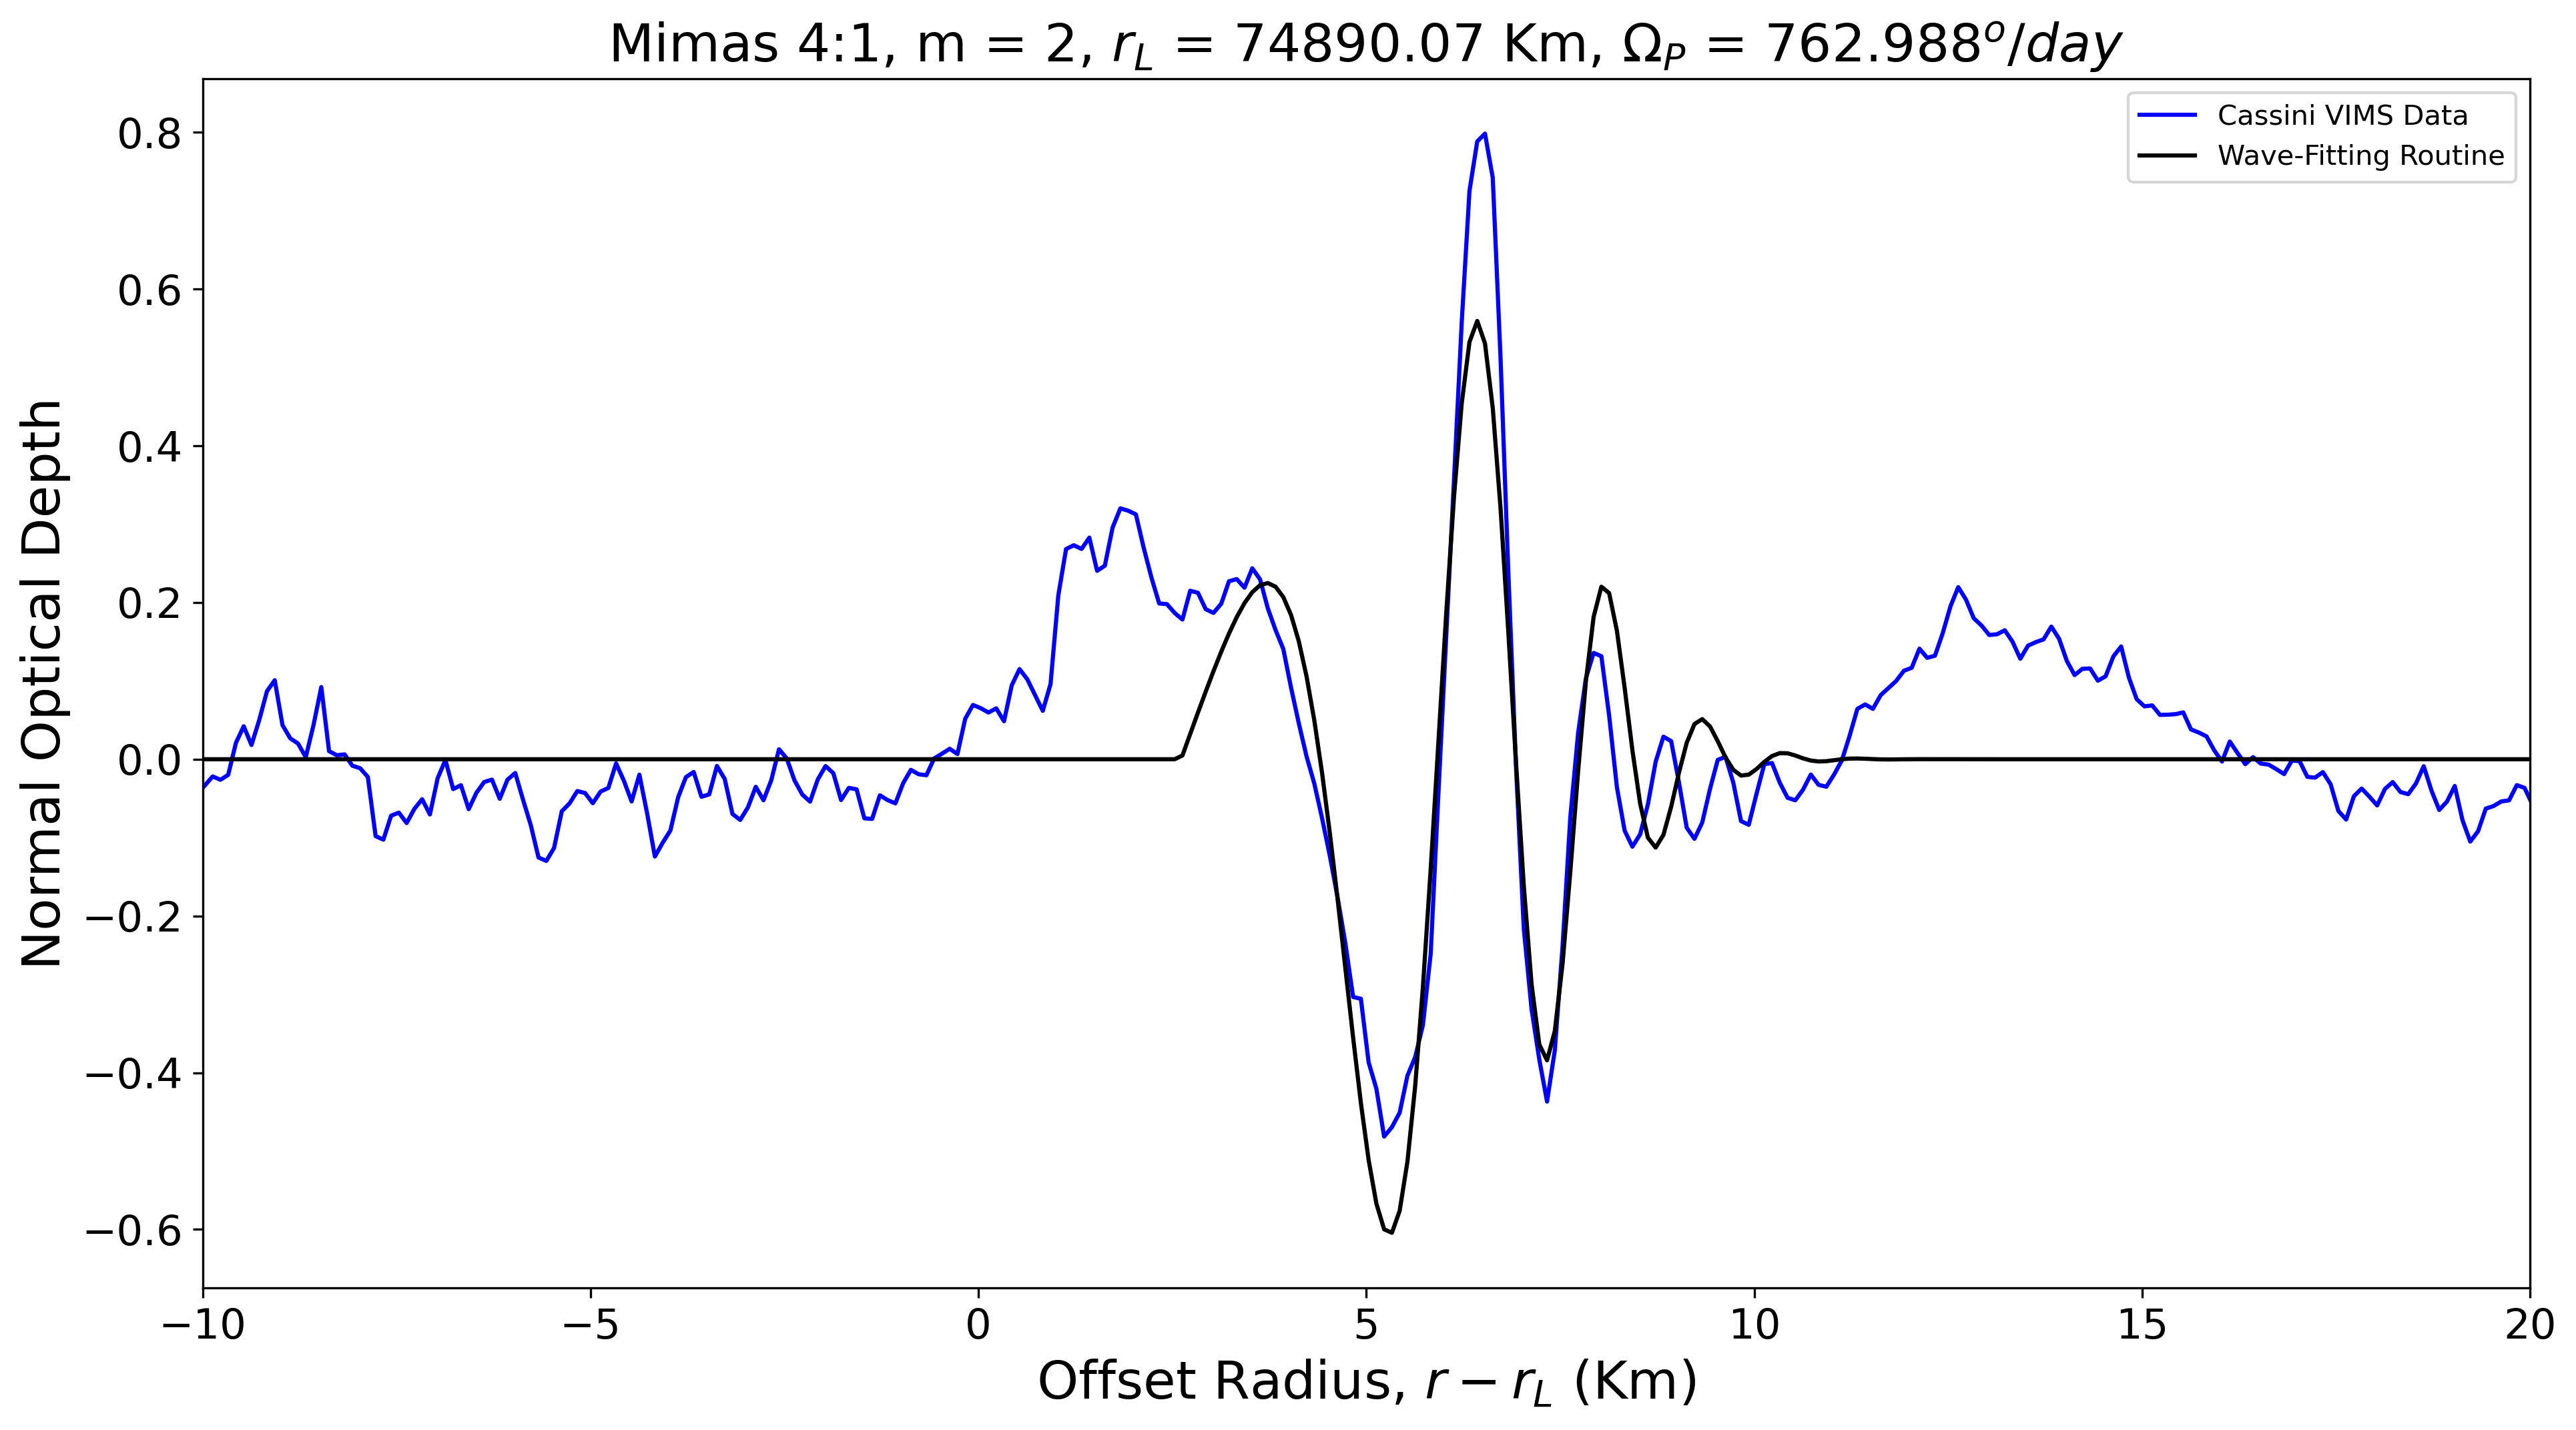
\includegraphics[width=0.3\textwidth, height=0.2\textheight, keepaspectratio]{mimas41.png}} &
        \subcaptionbox{Pan 2:1}{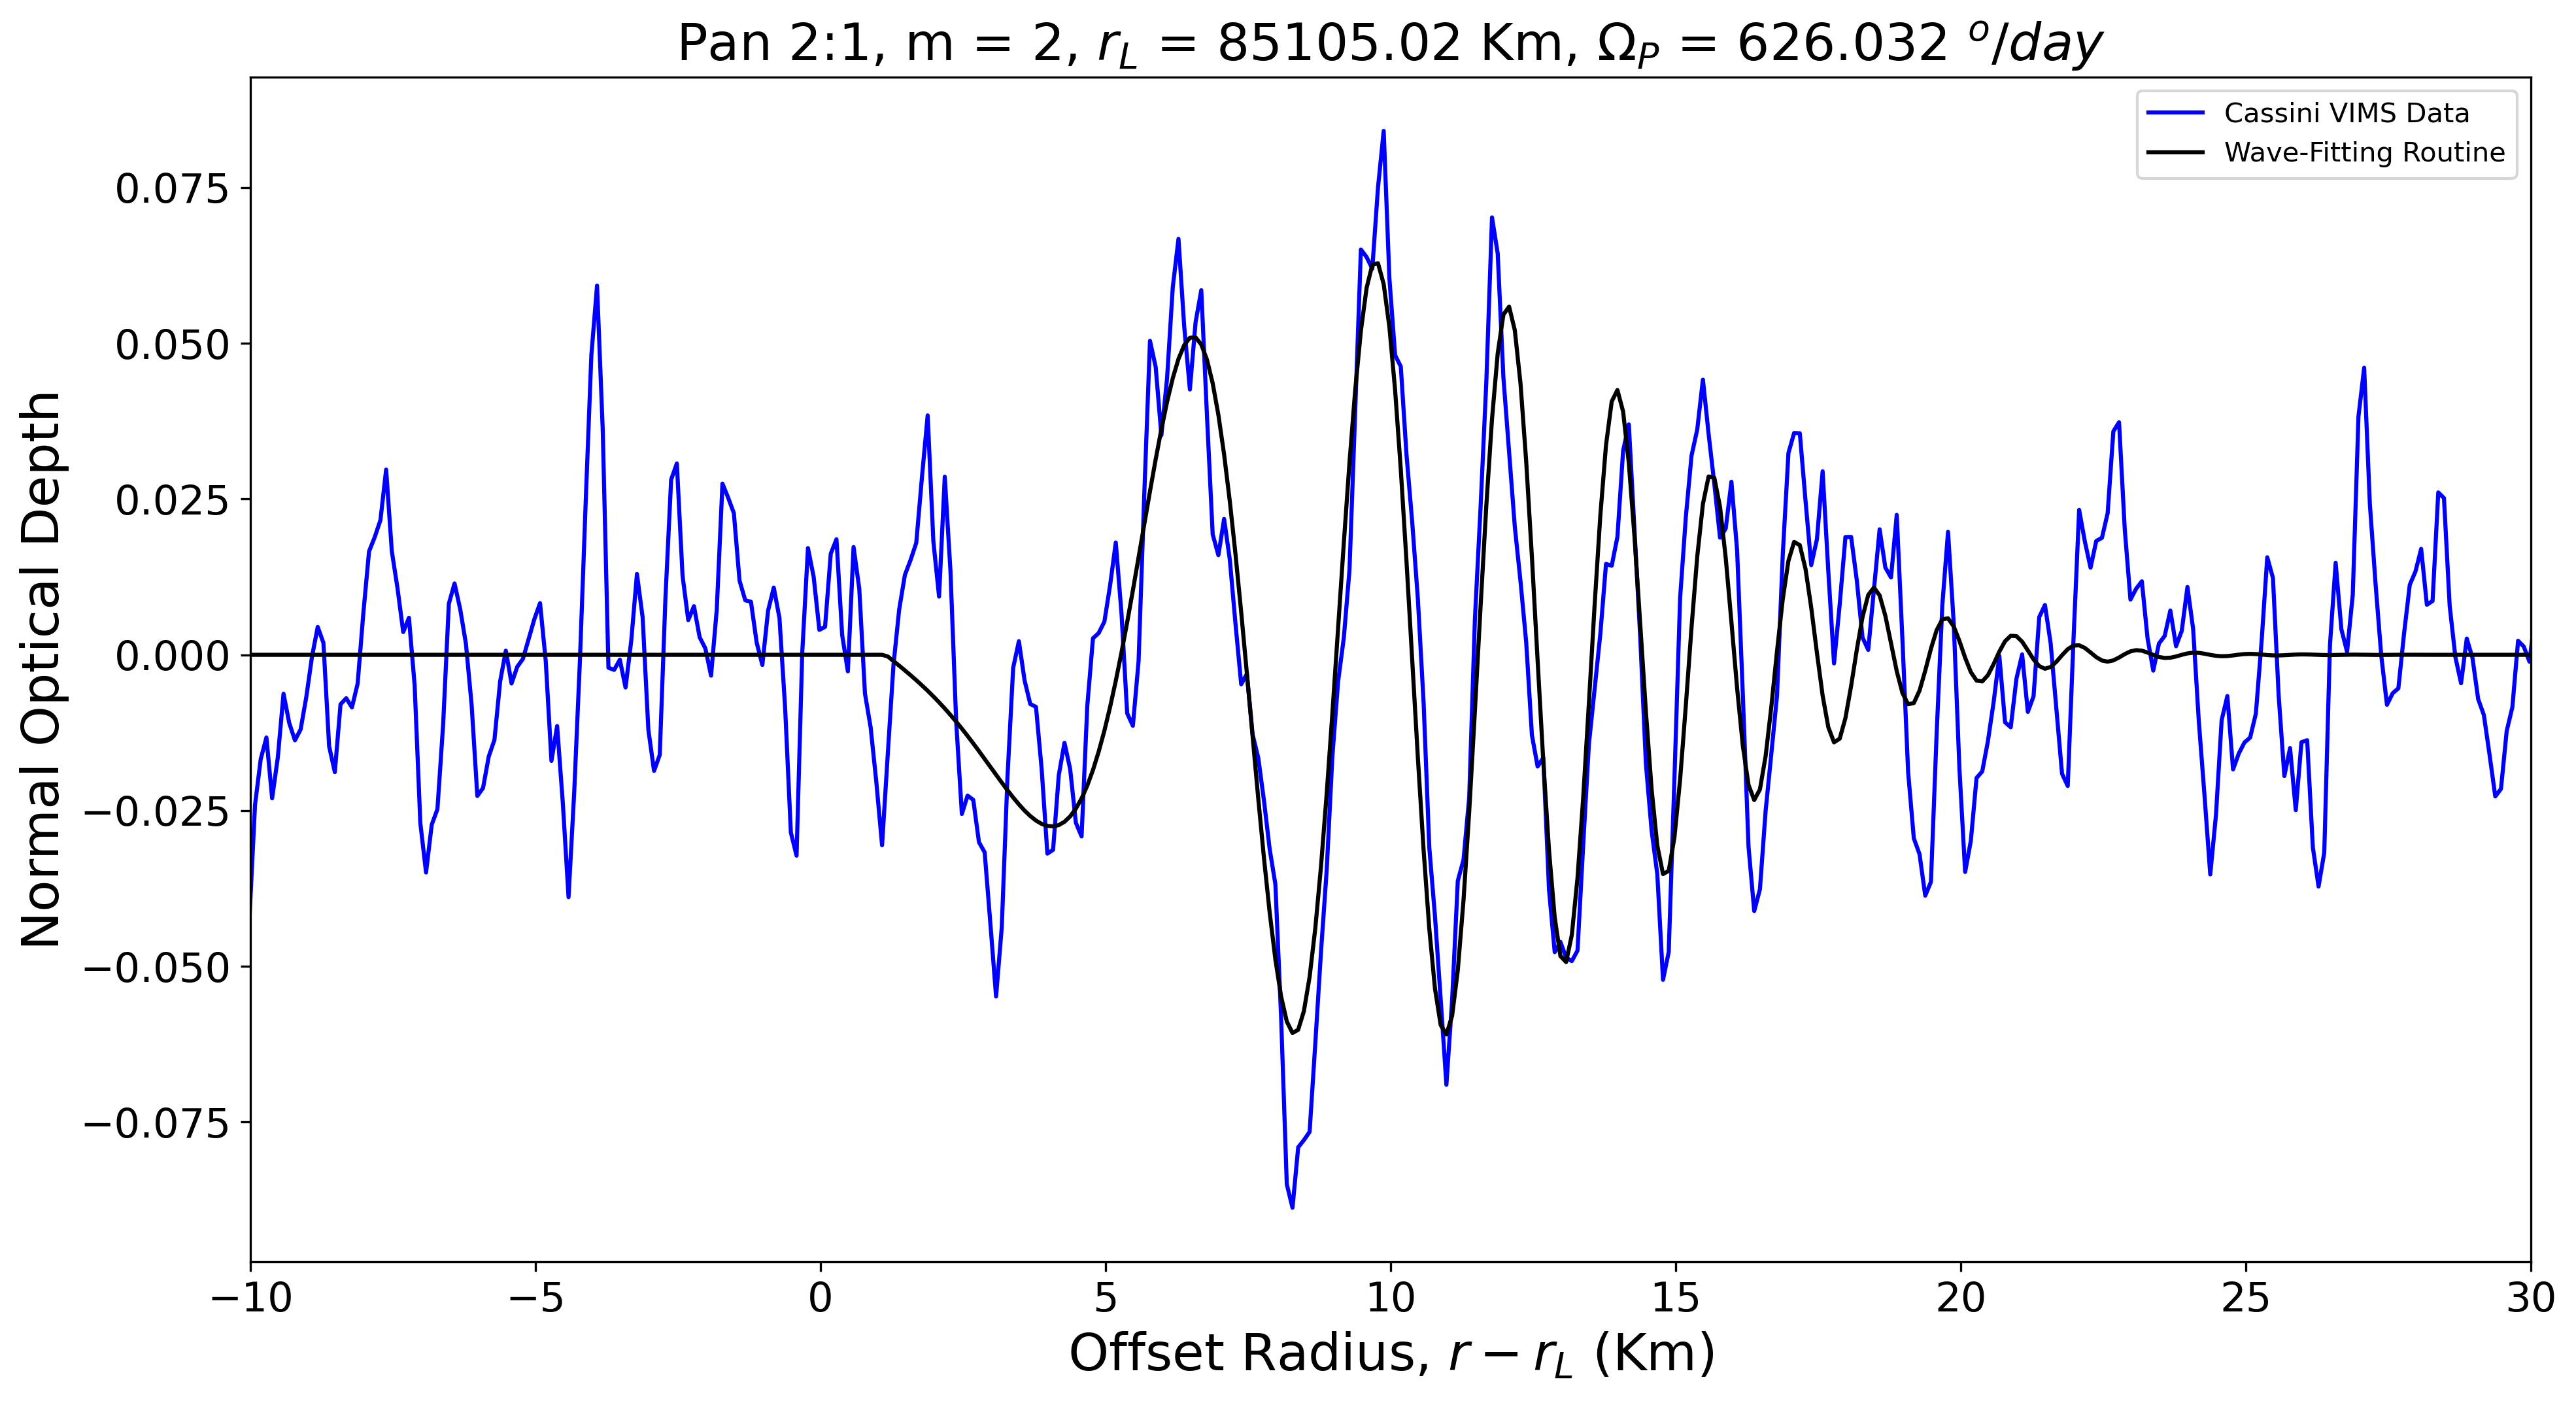
\includegraphics[width=0.3\textwidth, height=0.2\textheight, keepaspectratio]{pan21.png}} &        
        \subcaptionbox{Atlas 2:1}{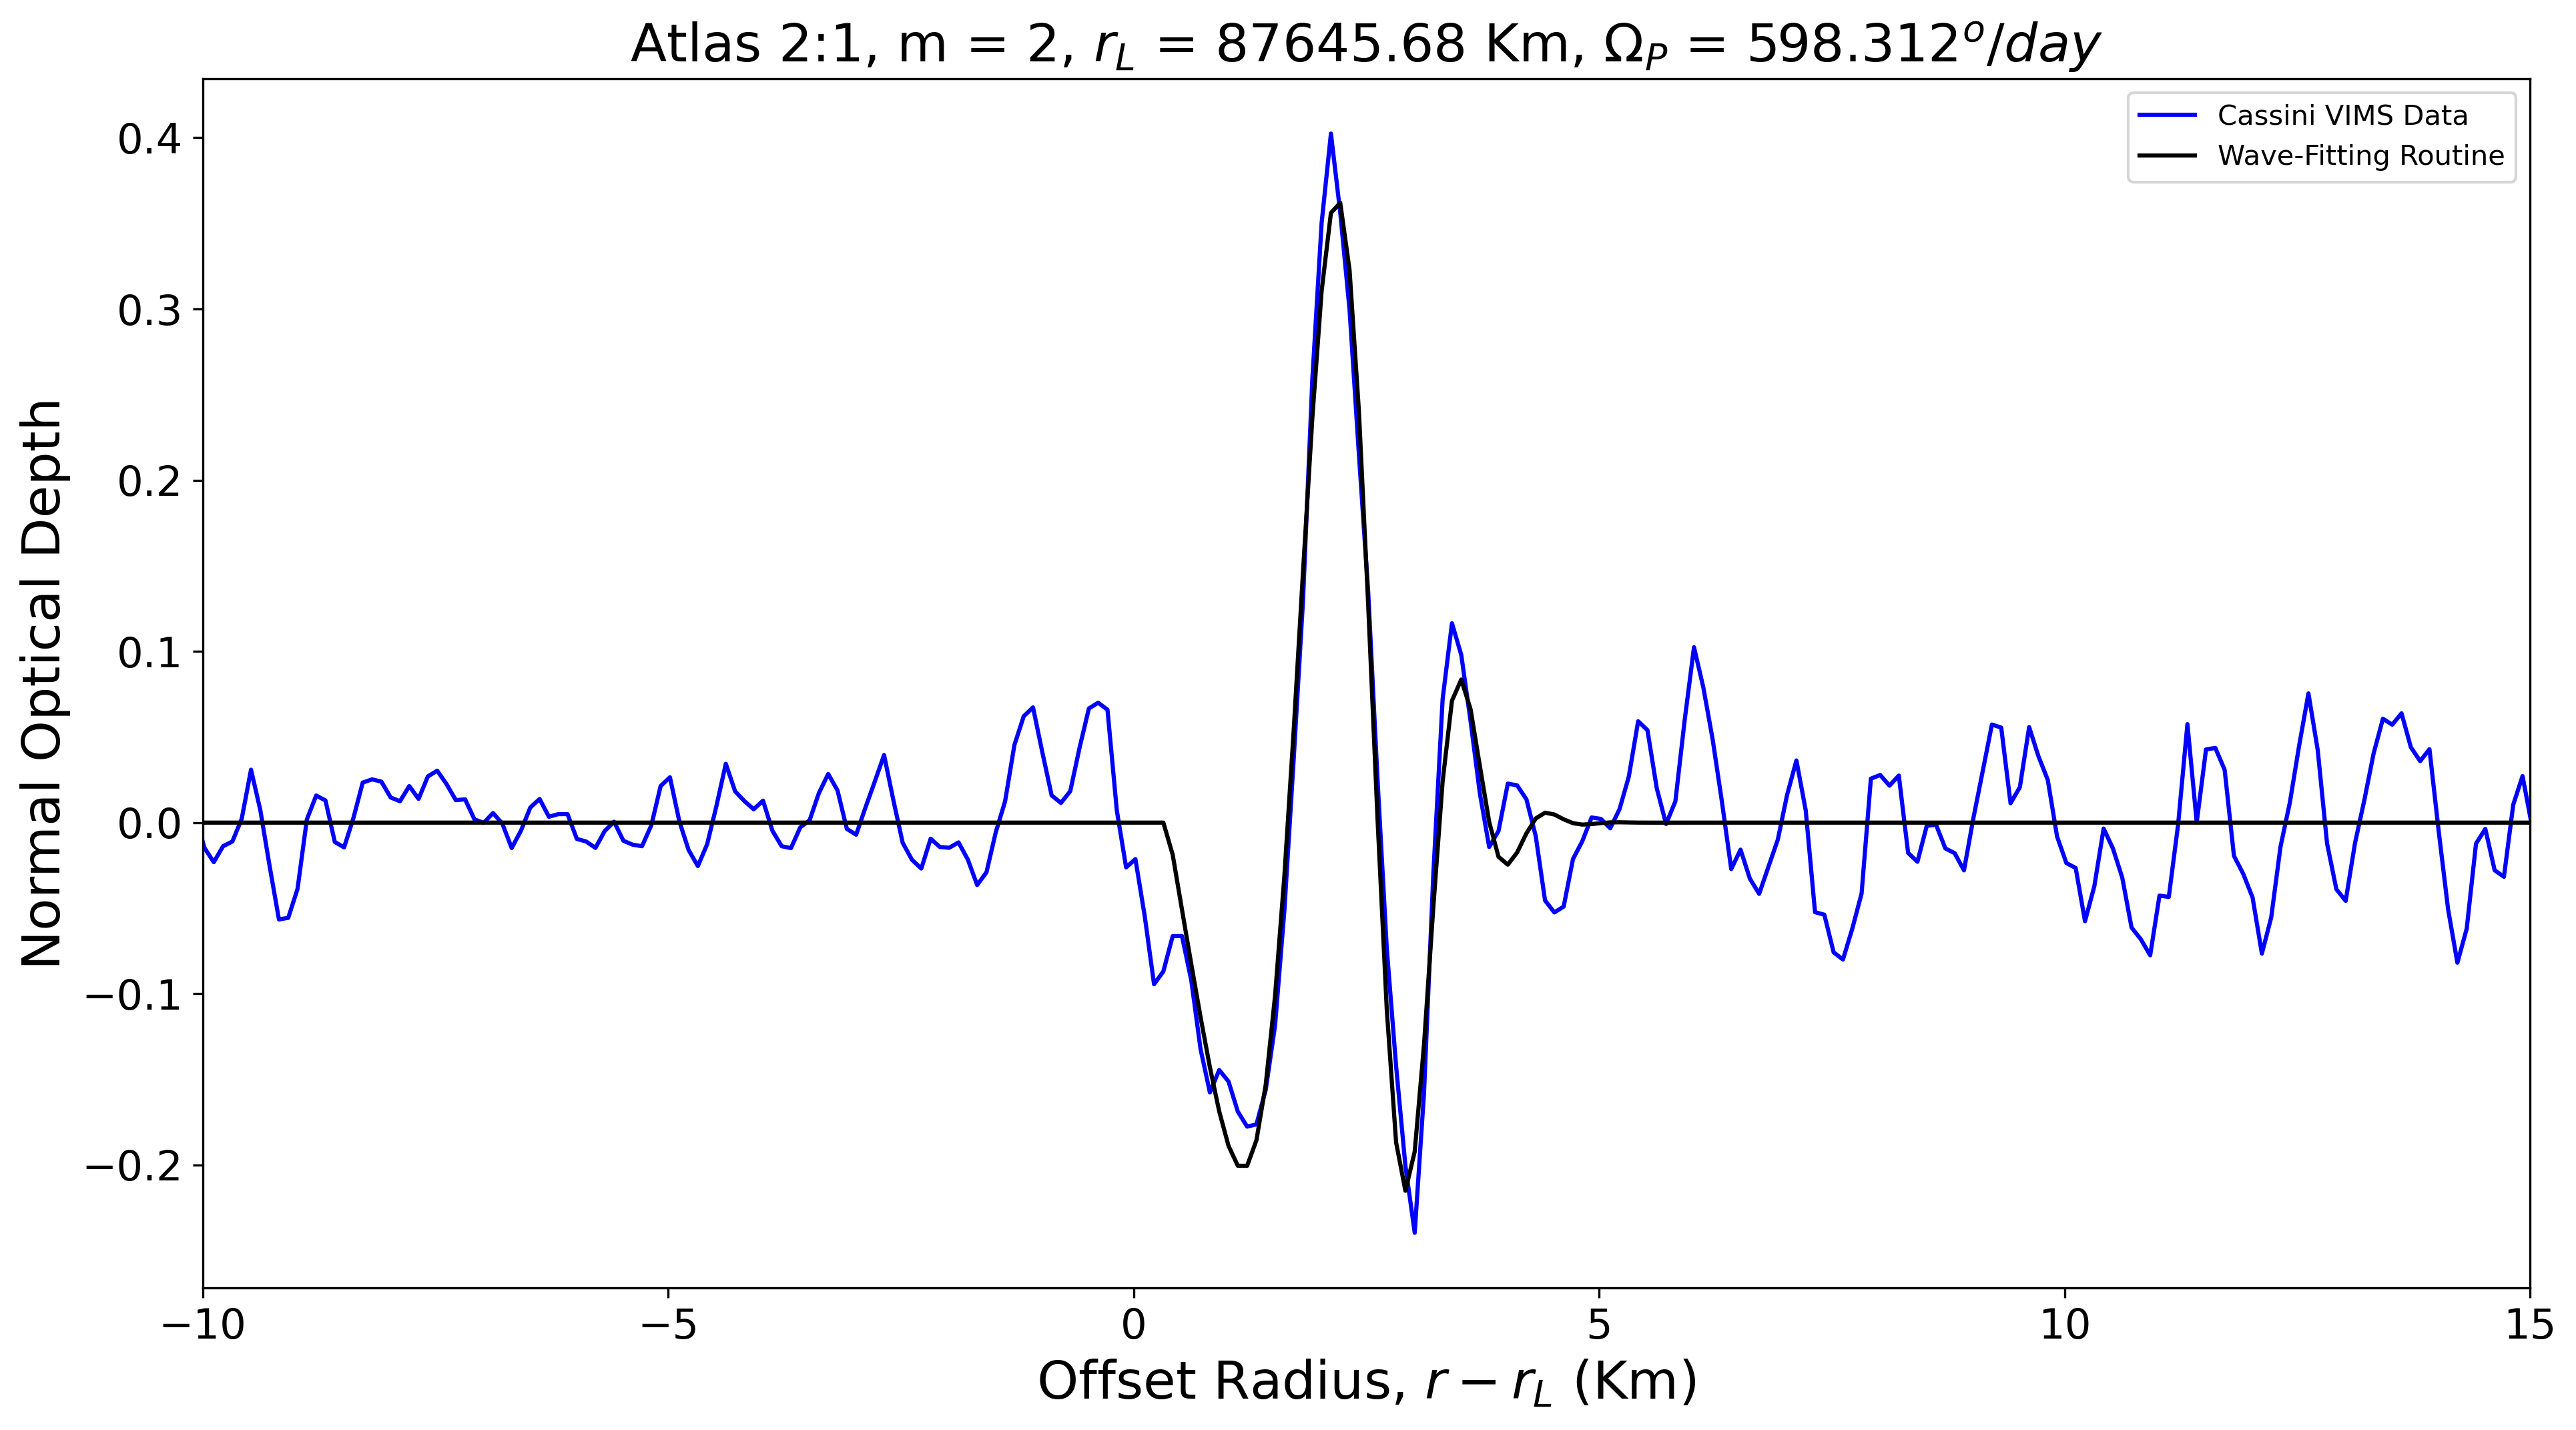
\includegraphics[width=0.3\textwidth, height=0.2\textheight, keepaspectratio]{atlas21.png}} \\        
        \subcaptionbox{Prometheus 4:2}{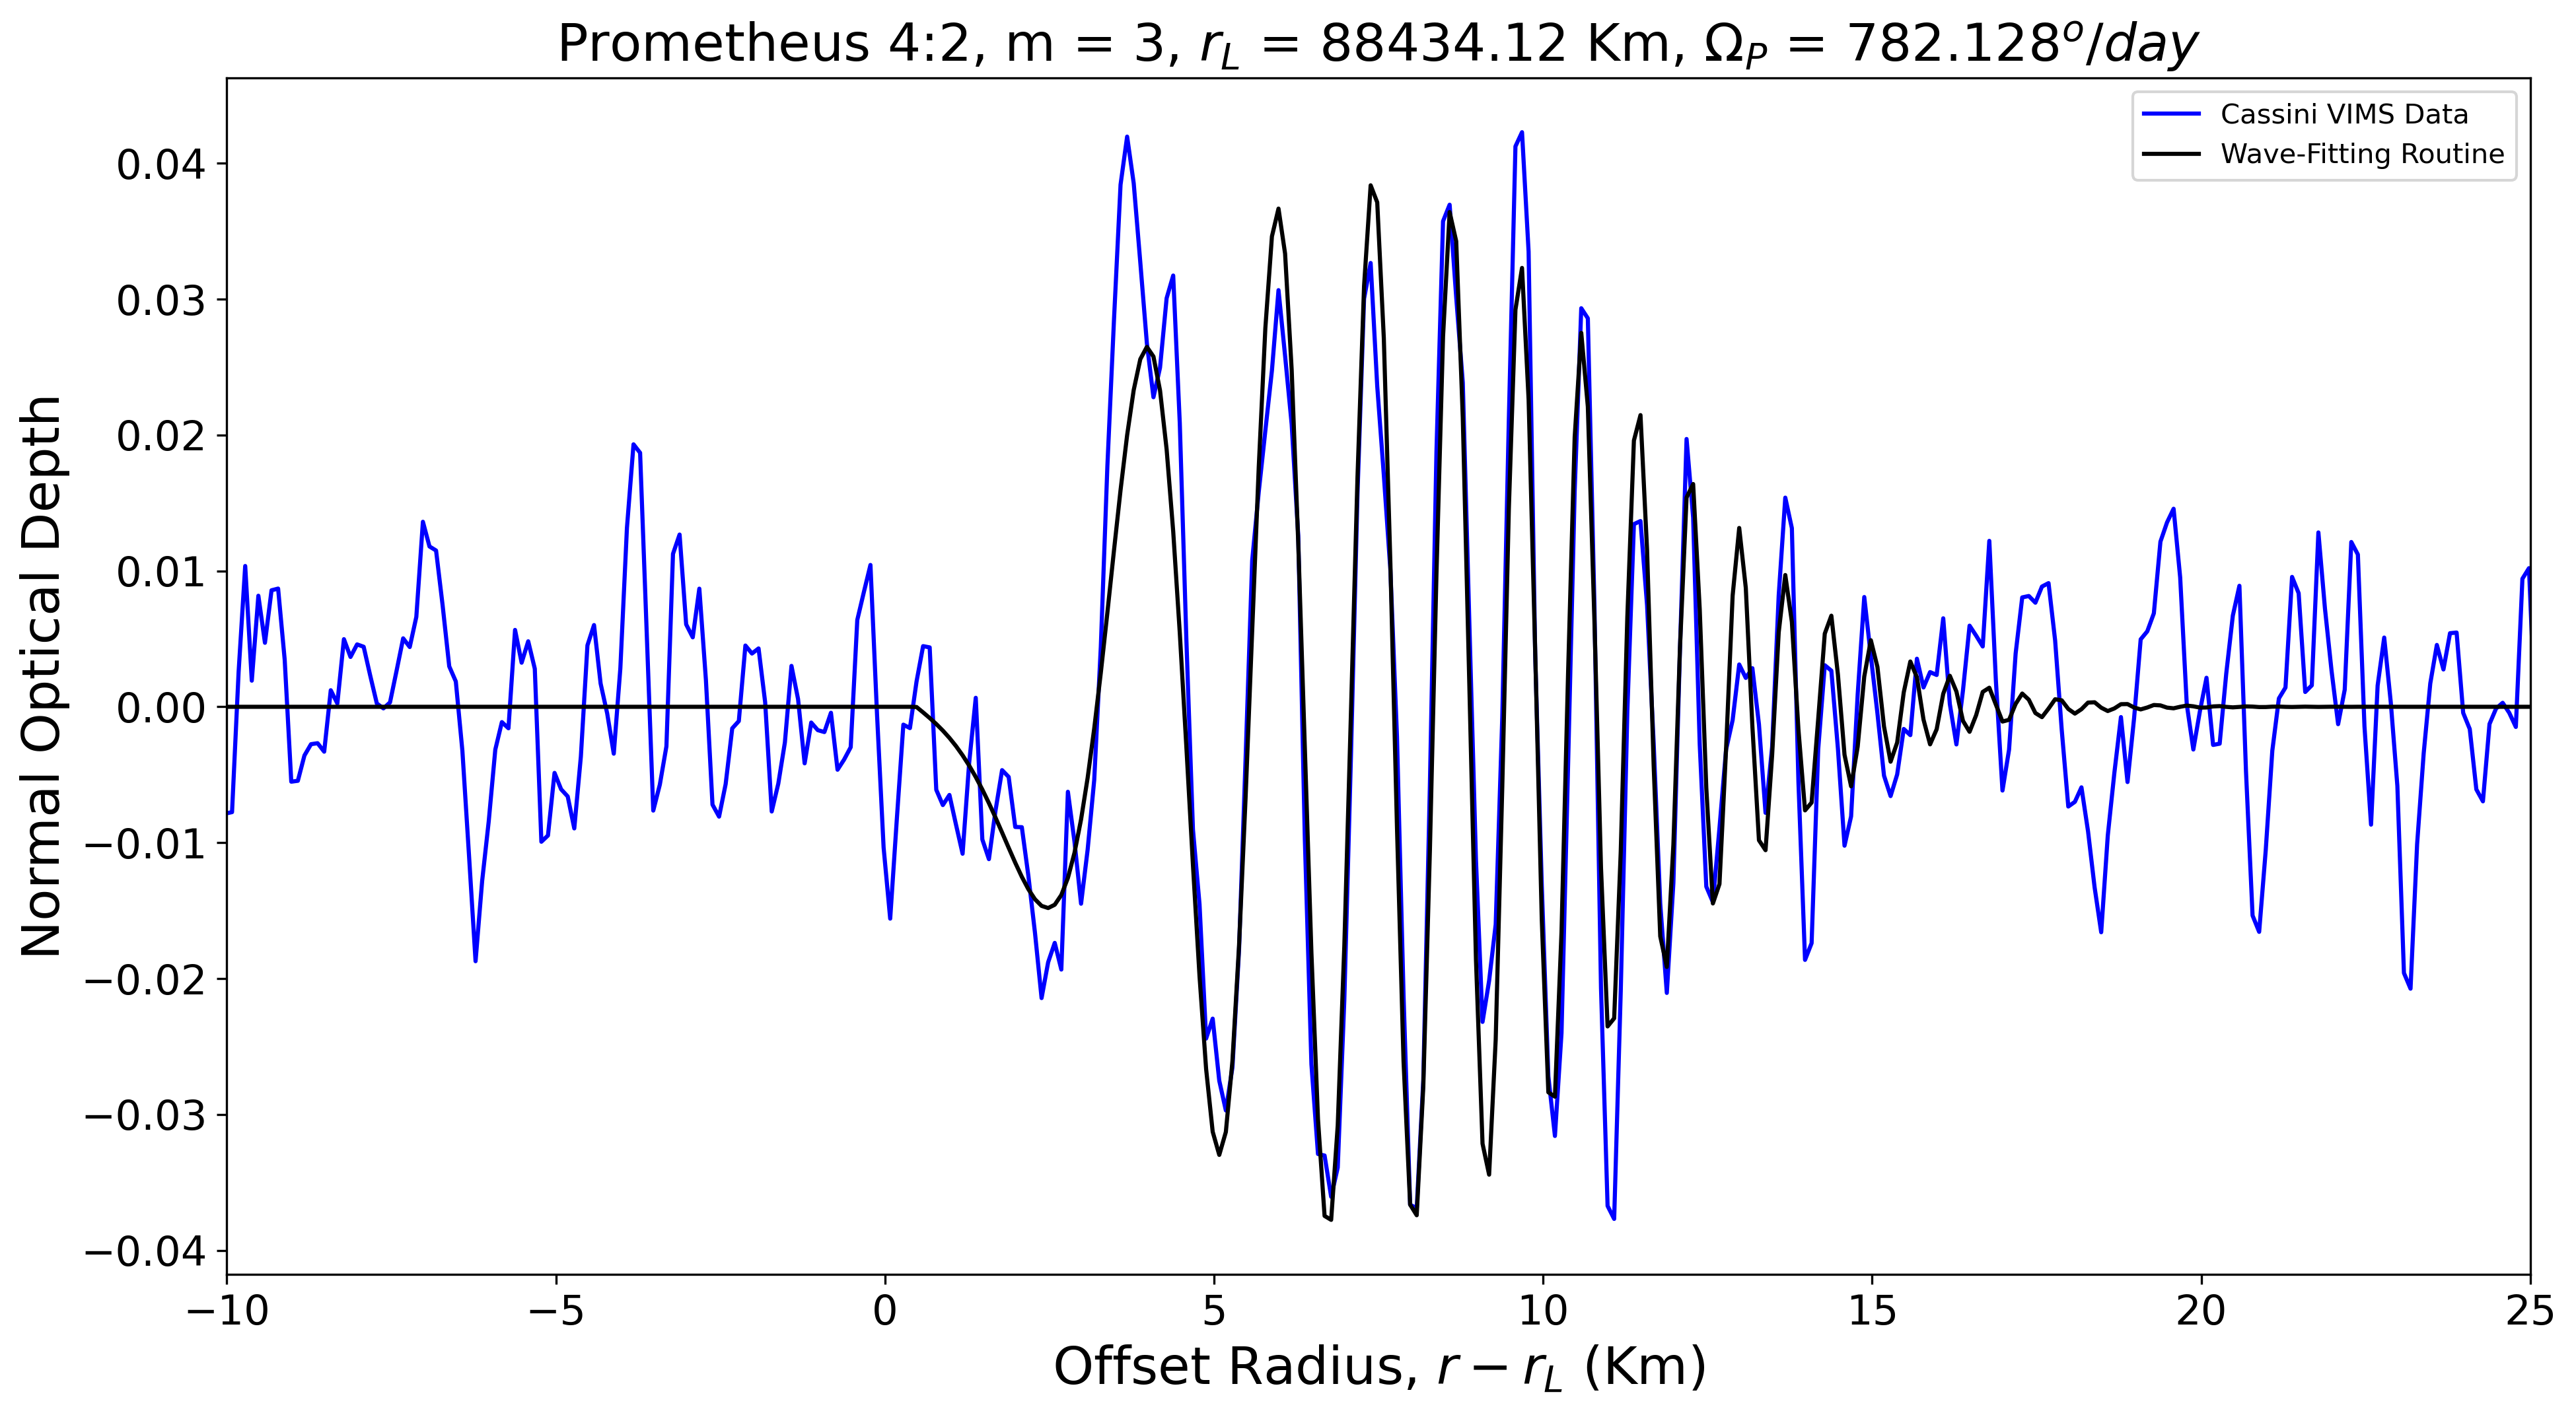
\includegraphics[width=0.3\textwidth, height=0.2\textheight, keepaspectratio]{prometheus42.png}} &        
        \subcaptionbox{Mimas 6:2}{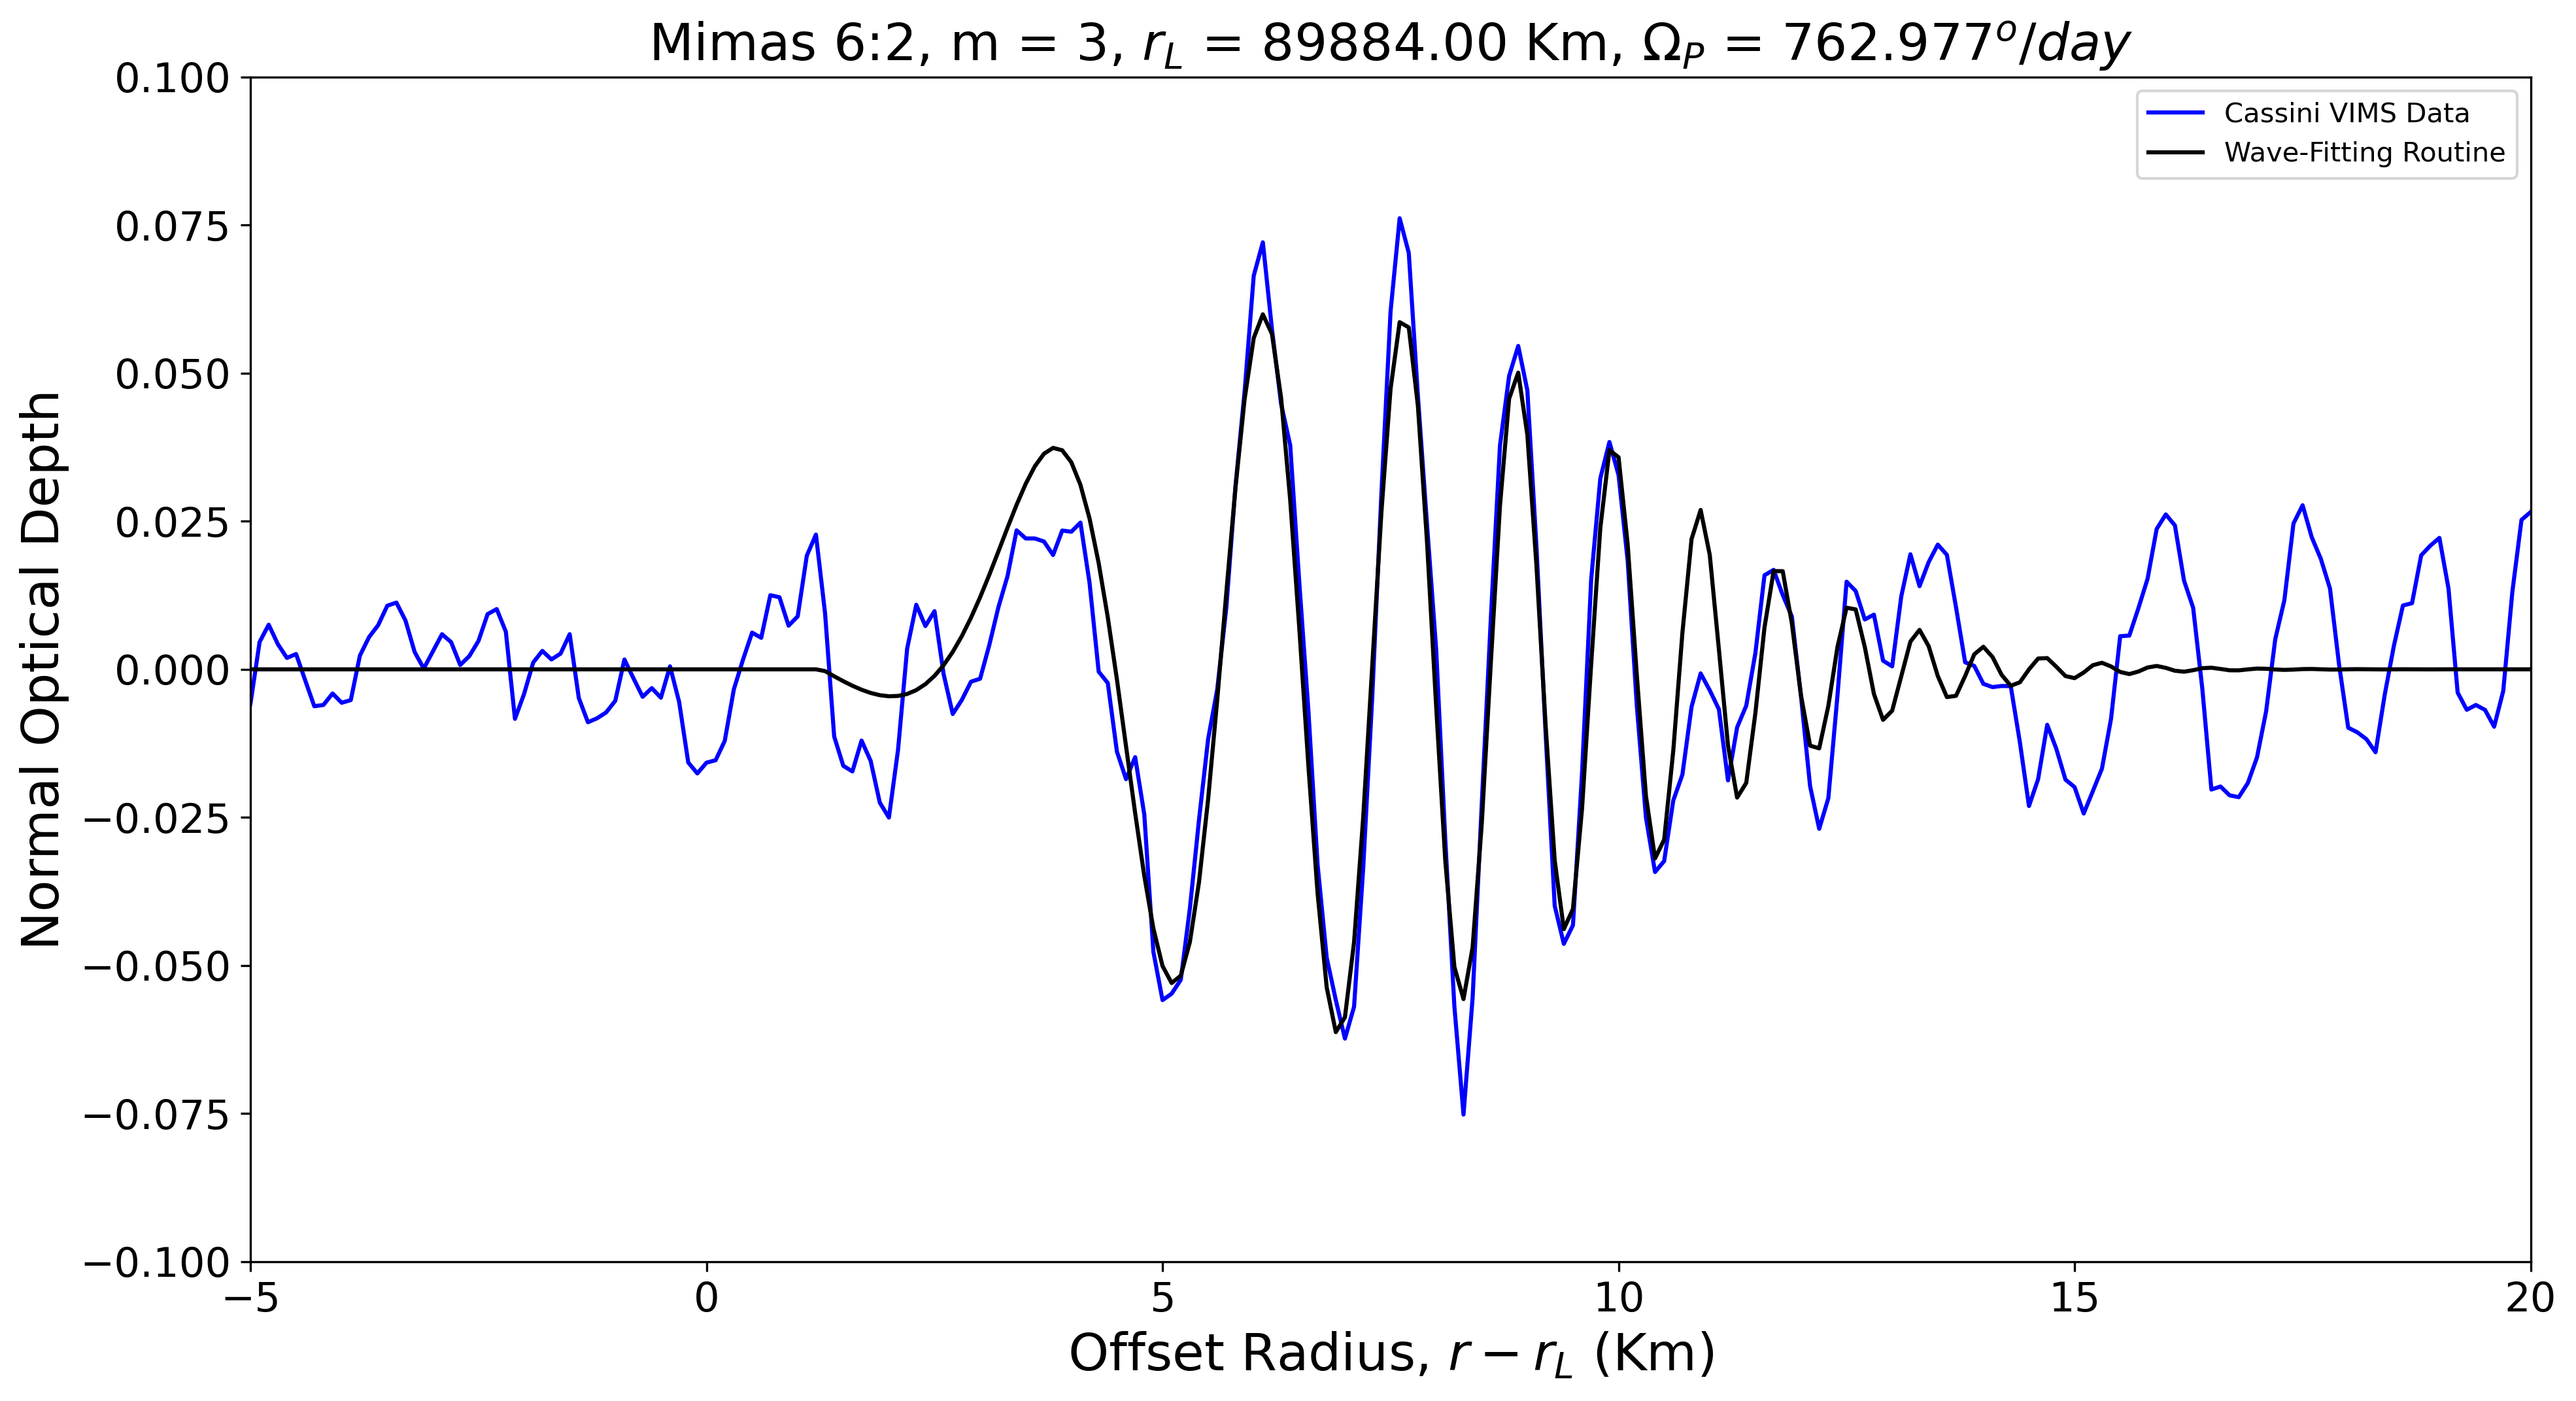
\includegraphics[width=0.3\textwidth, height=0.2\textheight, keepaspectratio]{mimas62.png}} &        
        \subcaptionbox{Pandora 4:2}{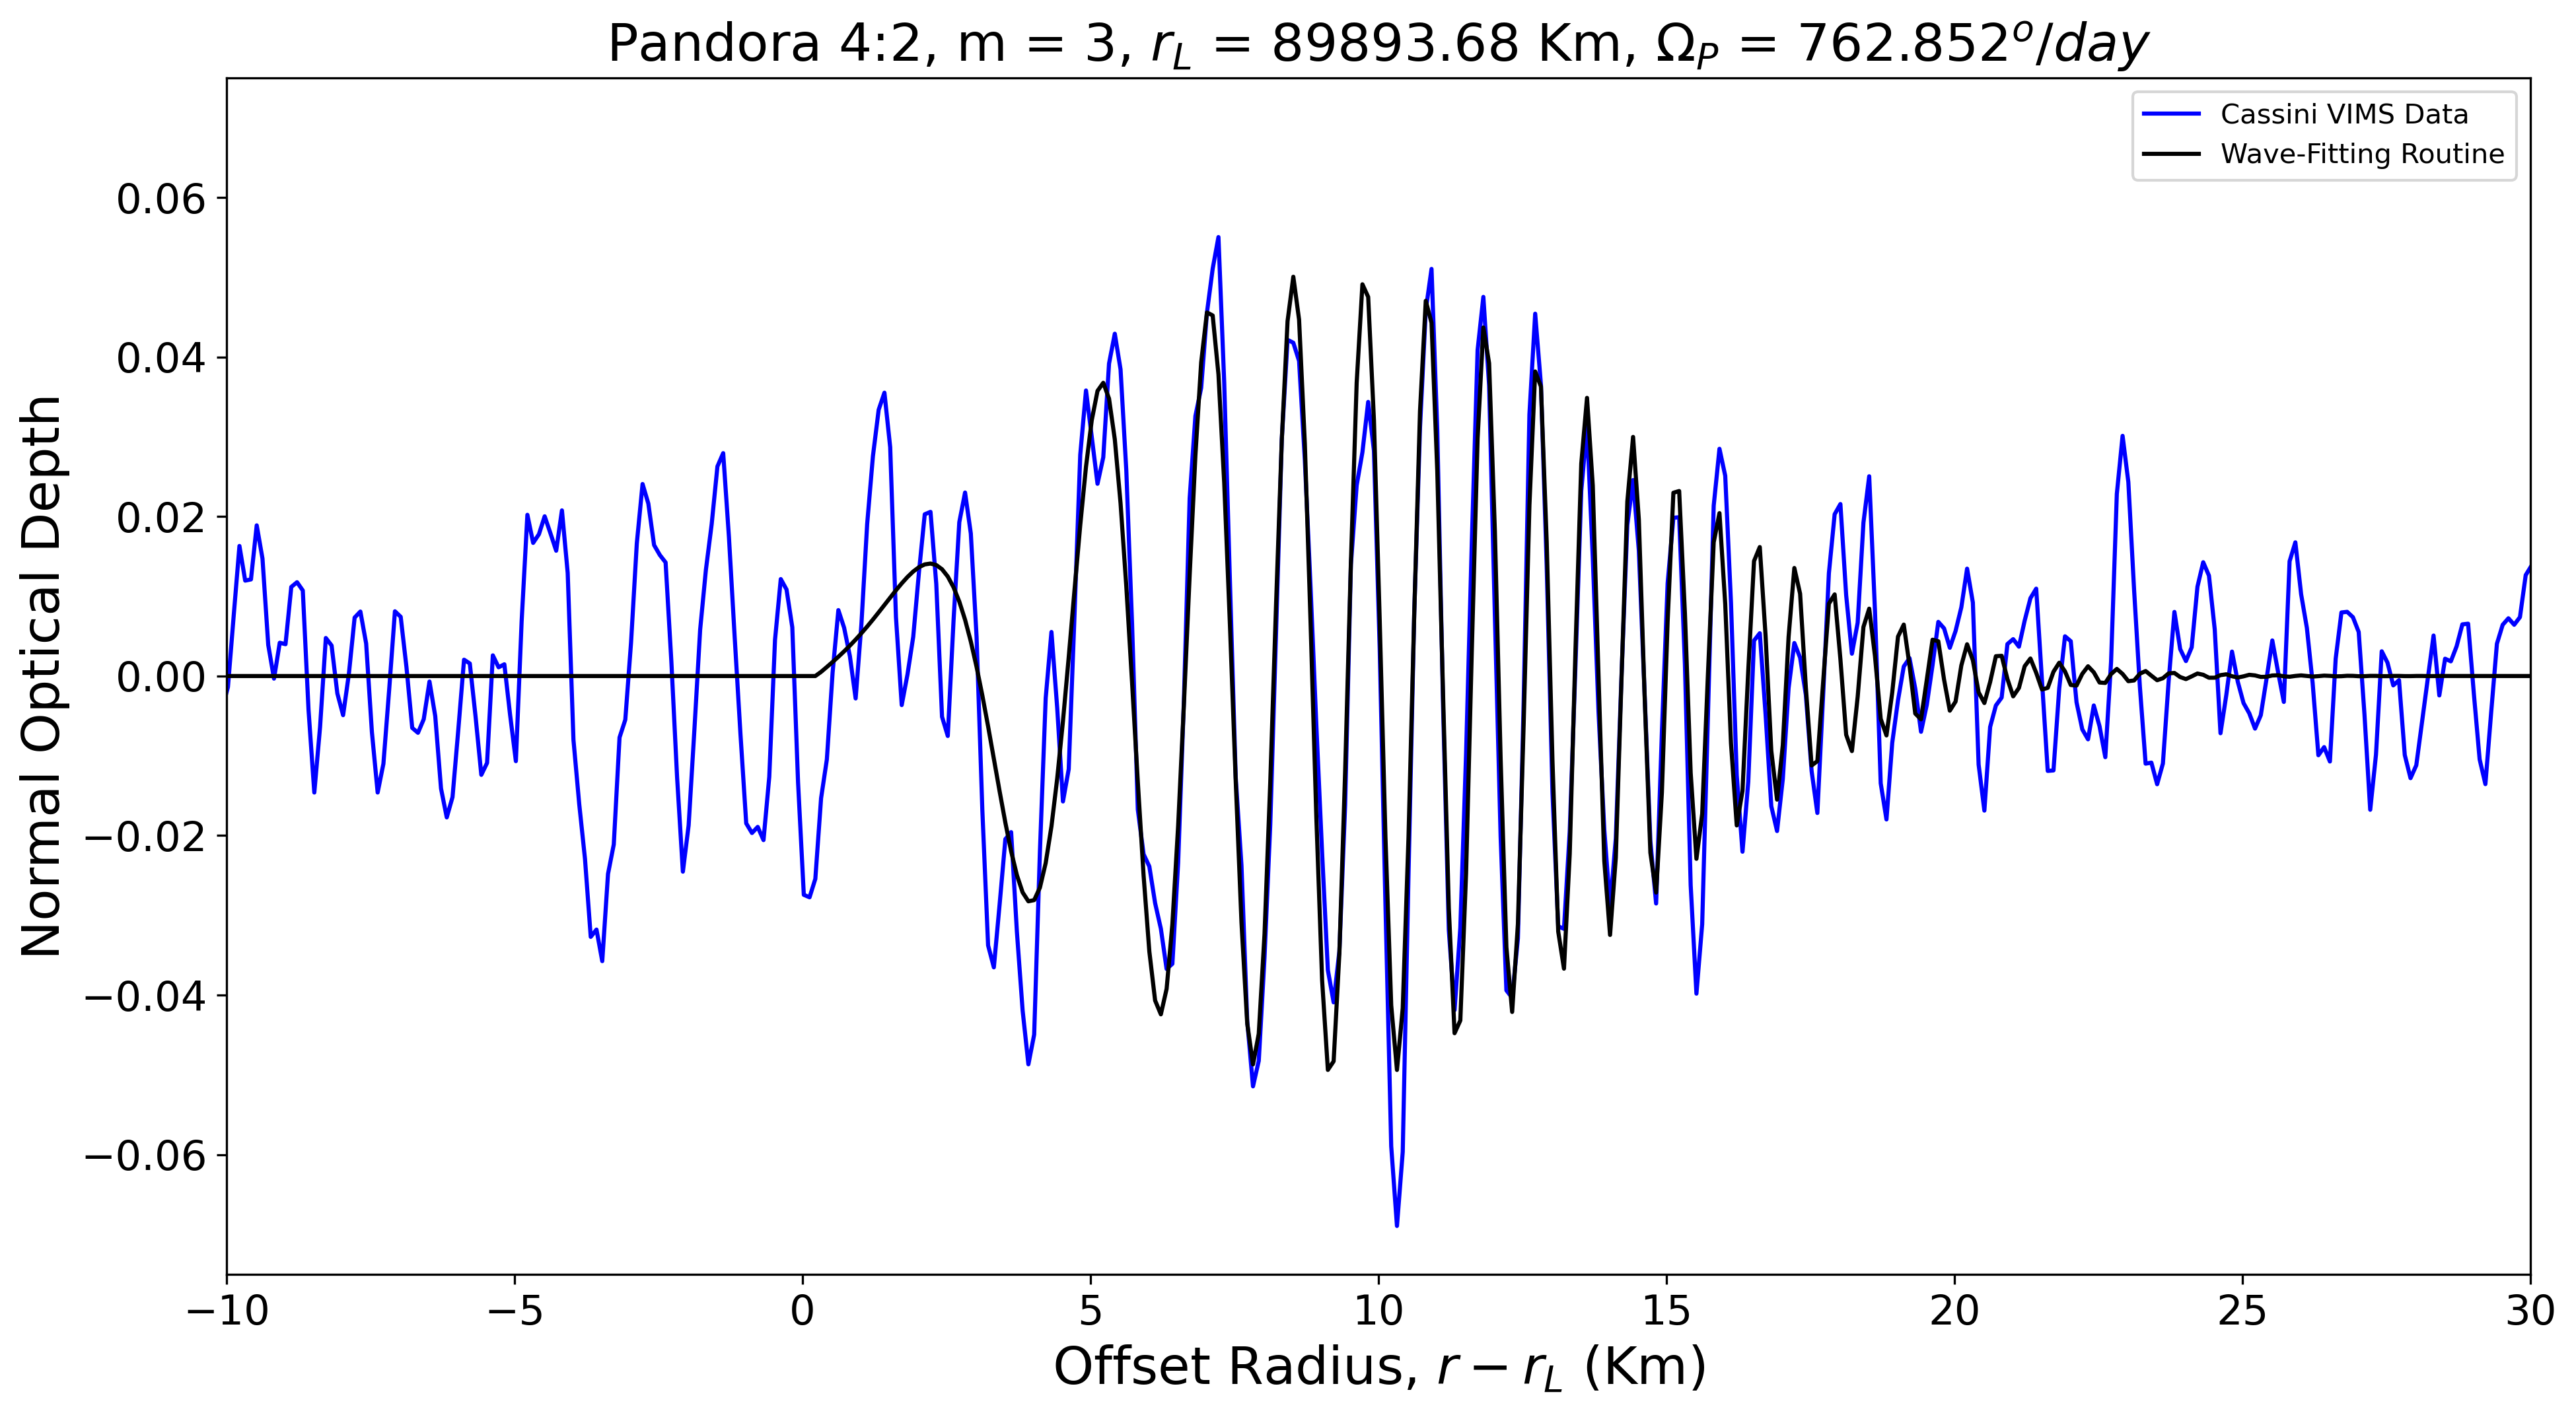
\includegraphics[width=0.3\textwidth, height=0.2\textheight, keepaspectratio]{pandora42.png}} \\        
        \subcaptionbox{$W74.51^{av}$}{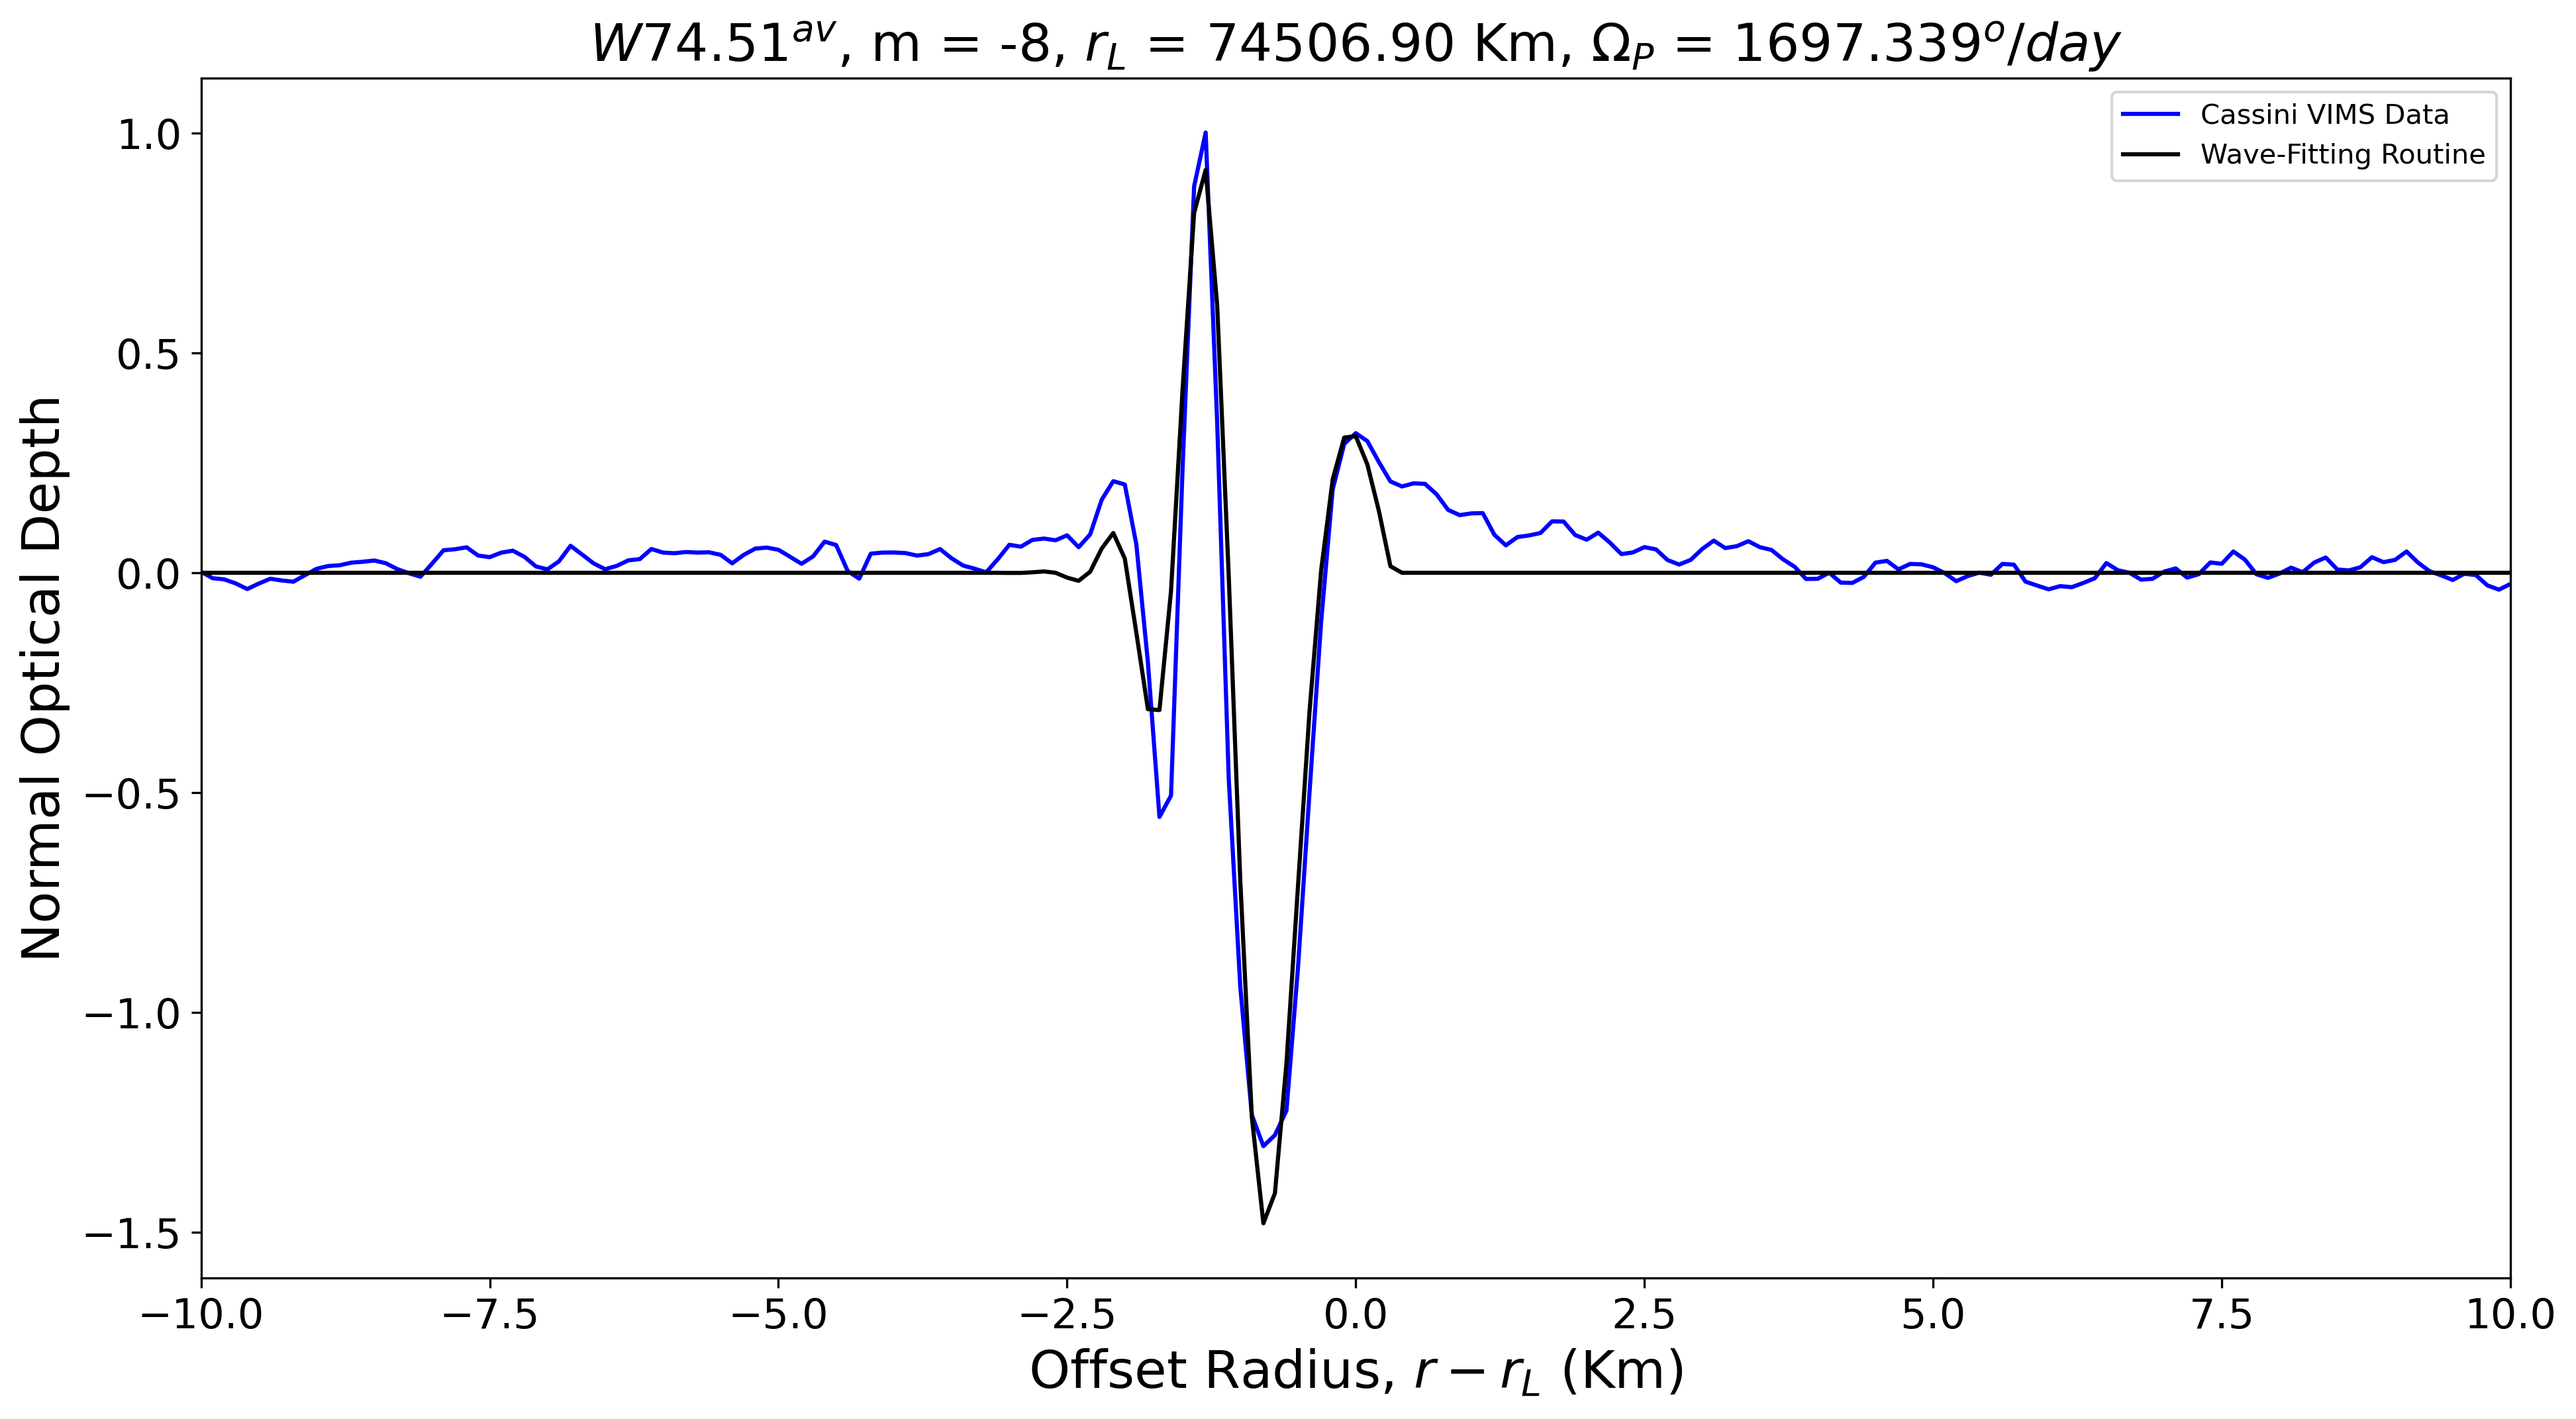
\includegraphics[width=0.3\textwidth, height=0.2\textheight, keepaspectratio]{w7451mp.png}} &
        \subcaptionbox{W74.74}{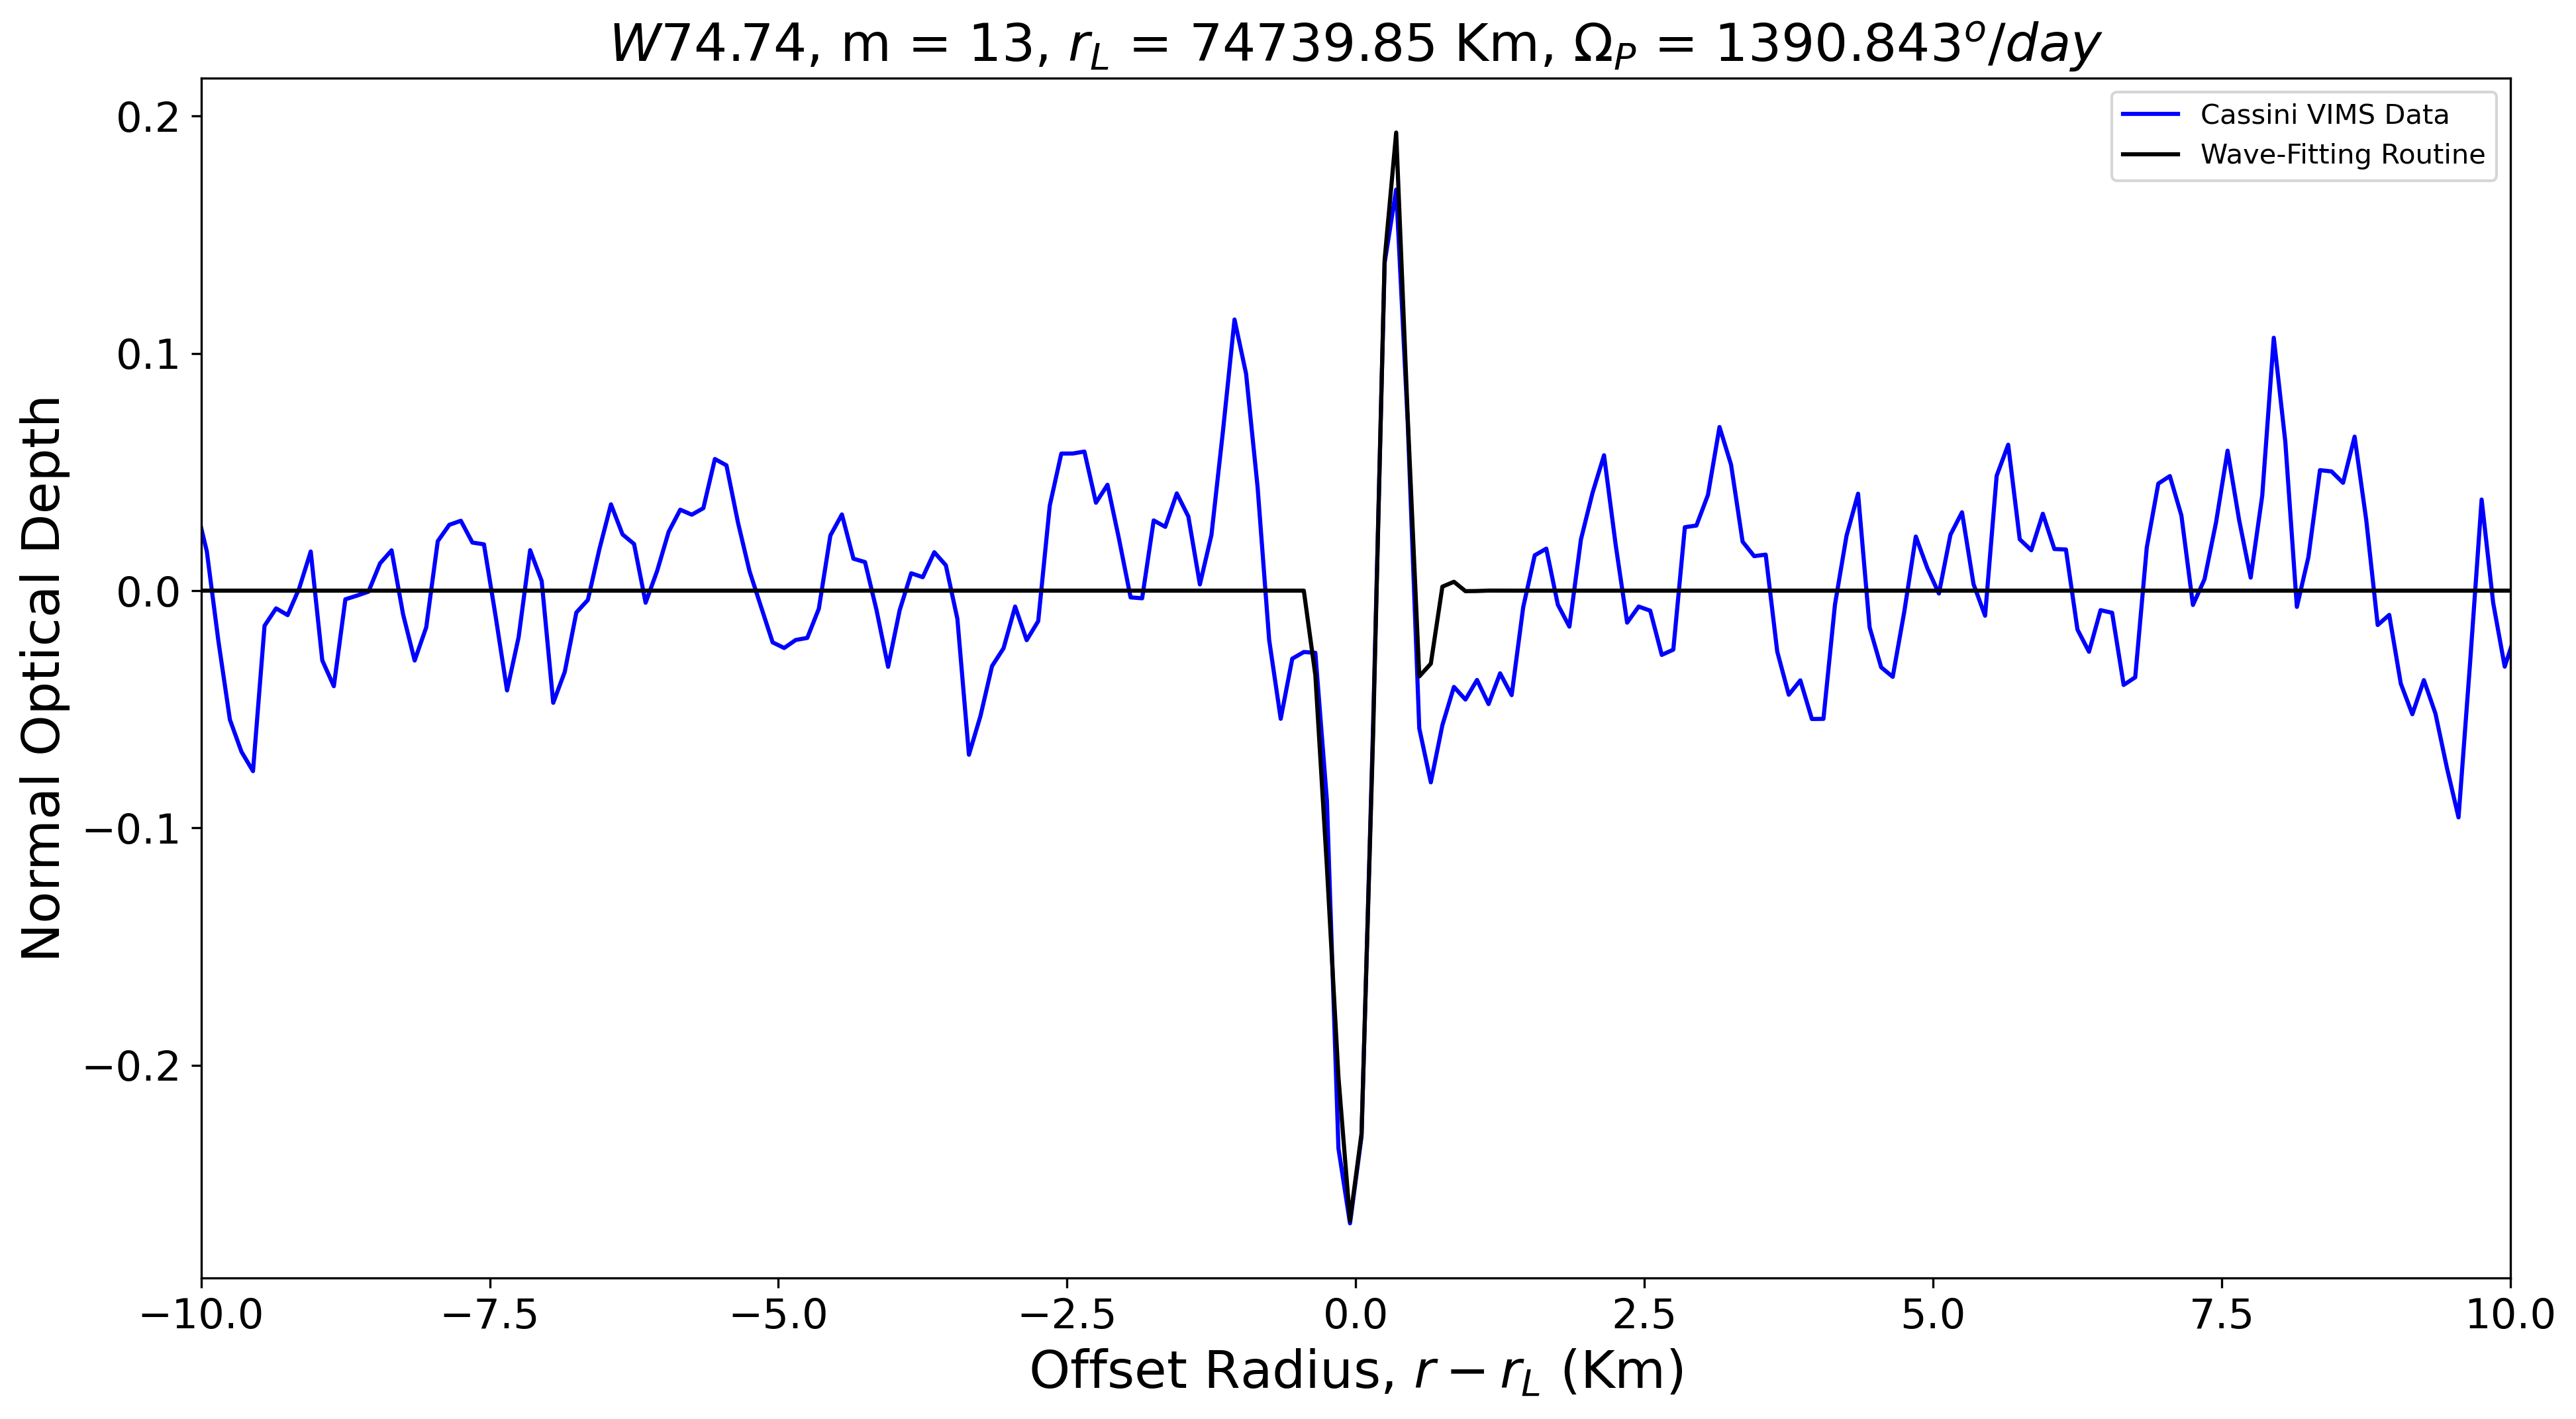
\includegraphics[width=0.3\textwidth, height=0.2\textheight, keepaspectratio]{w7474mp.png}} &
        \subcaptionbox{W74.75}{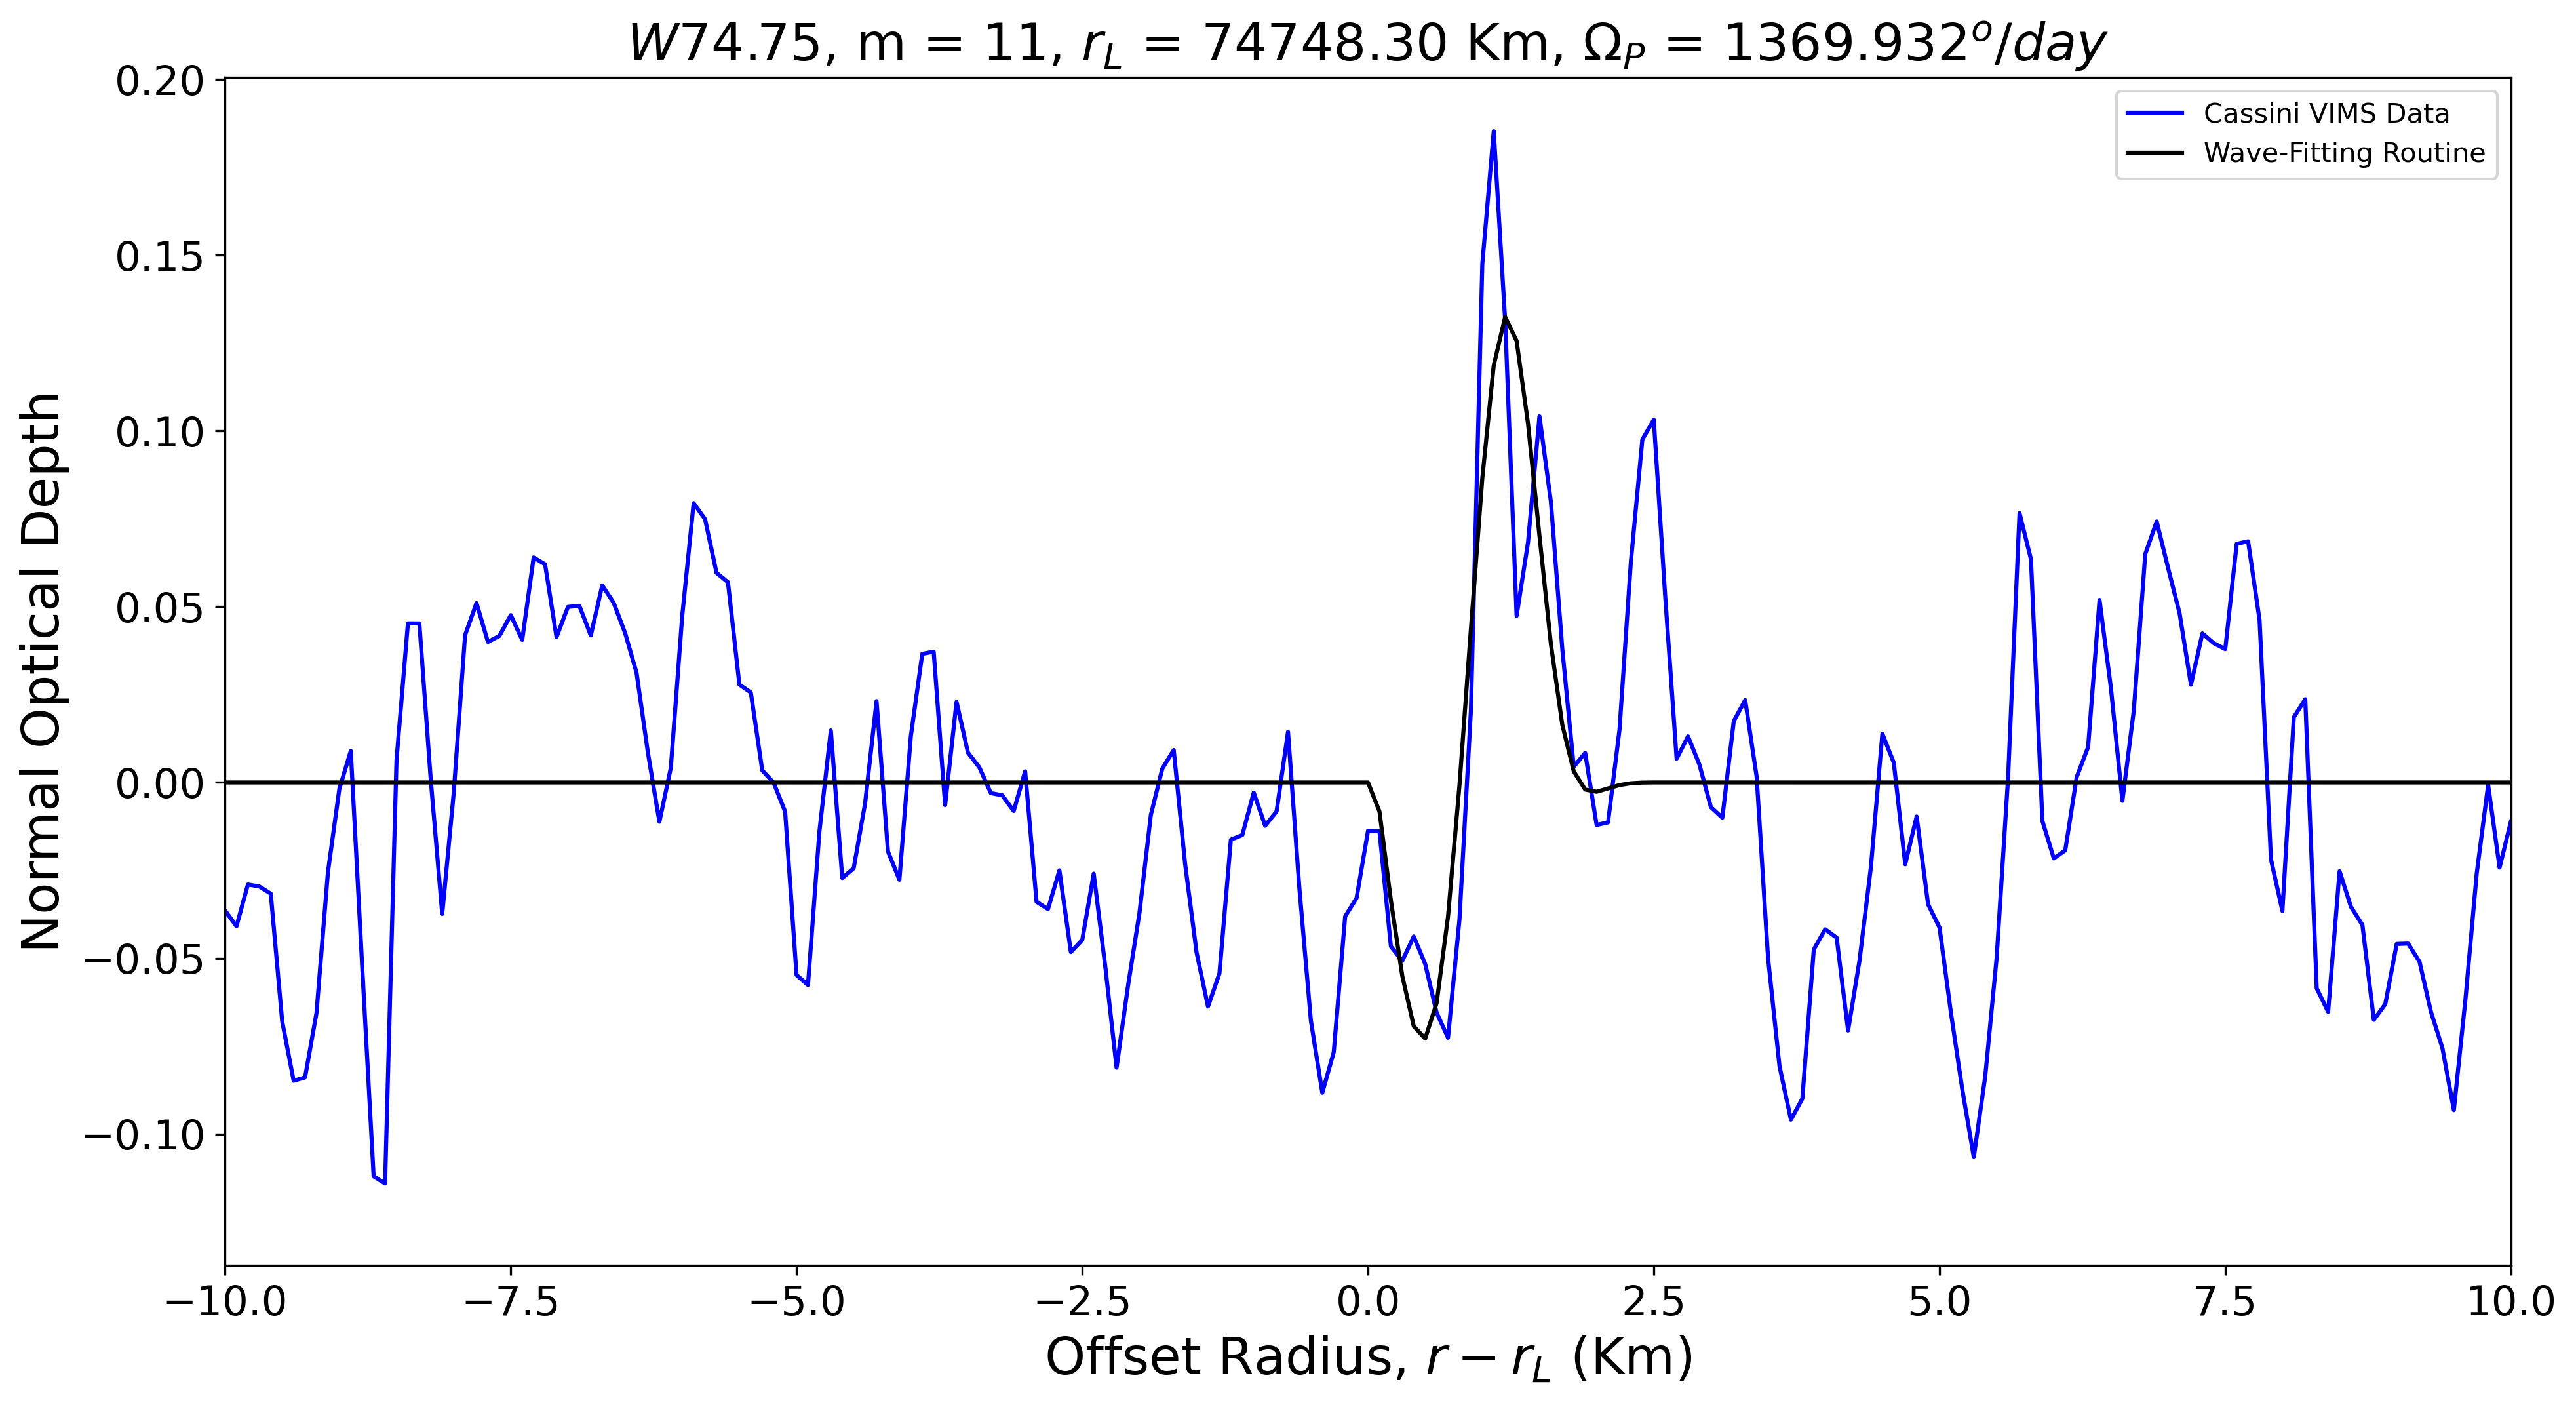
\includegraphics[width=0.3\textwidth, height=0.2\textheight, keepaspectratio]{w7475mp.png}} \\
        \subcaptionbox{W74.76}{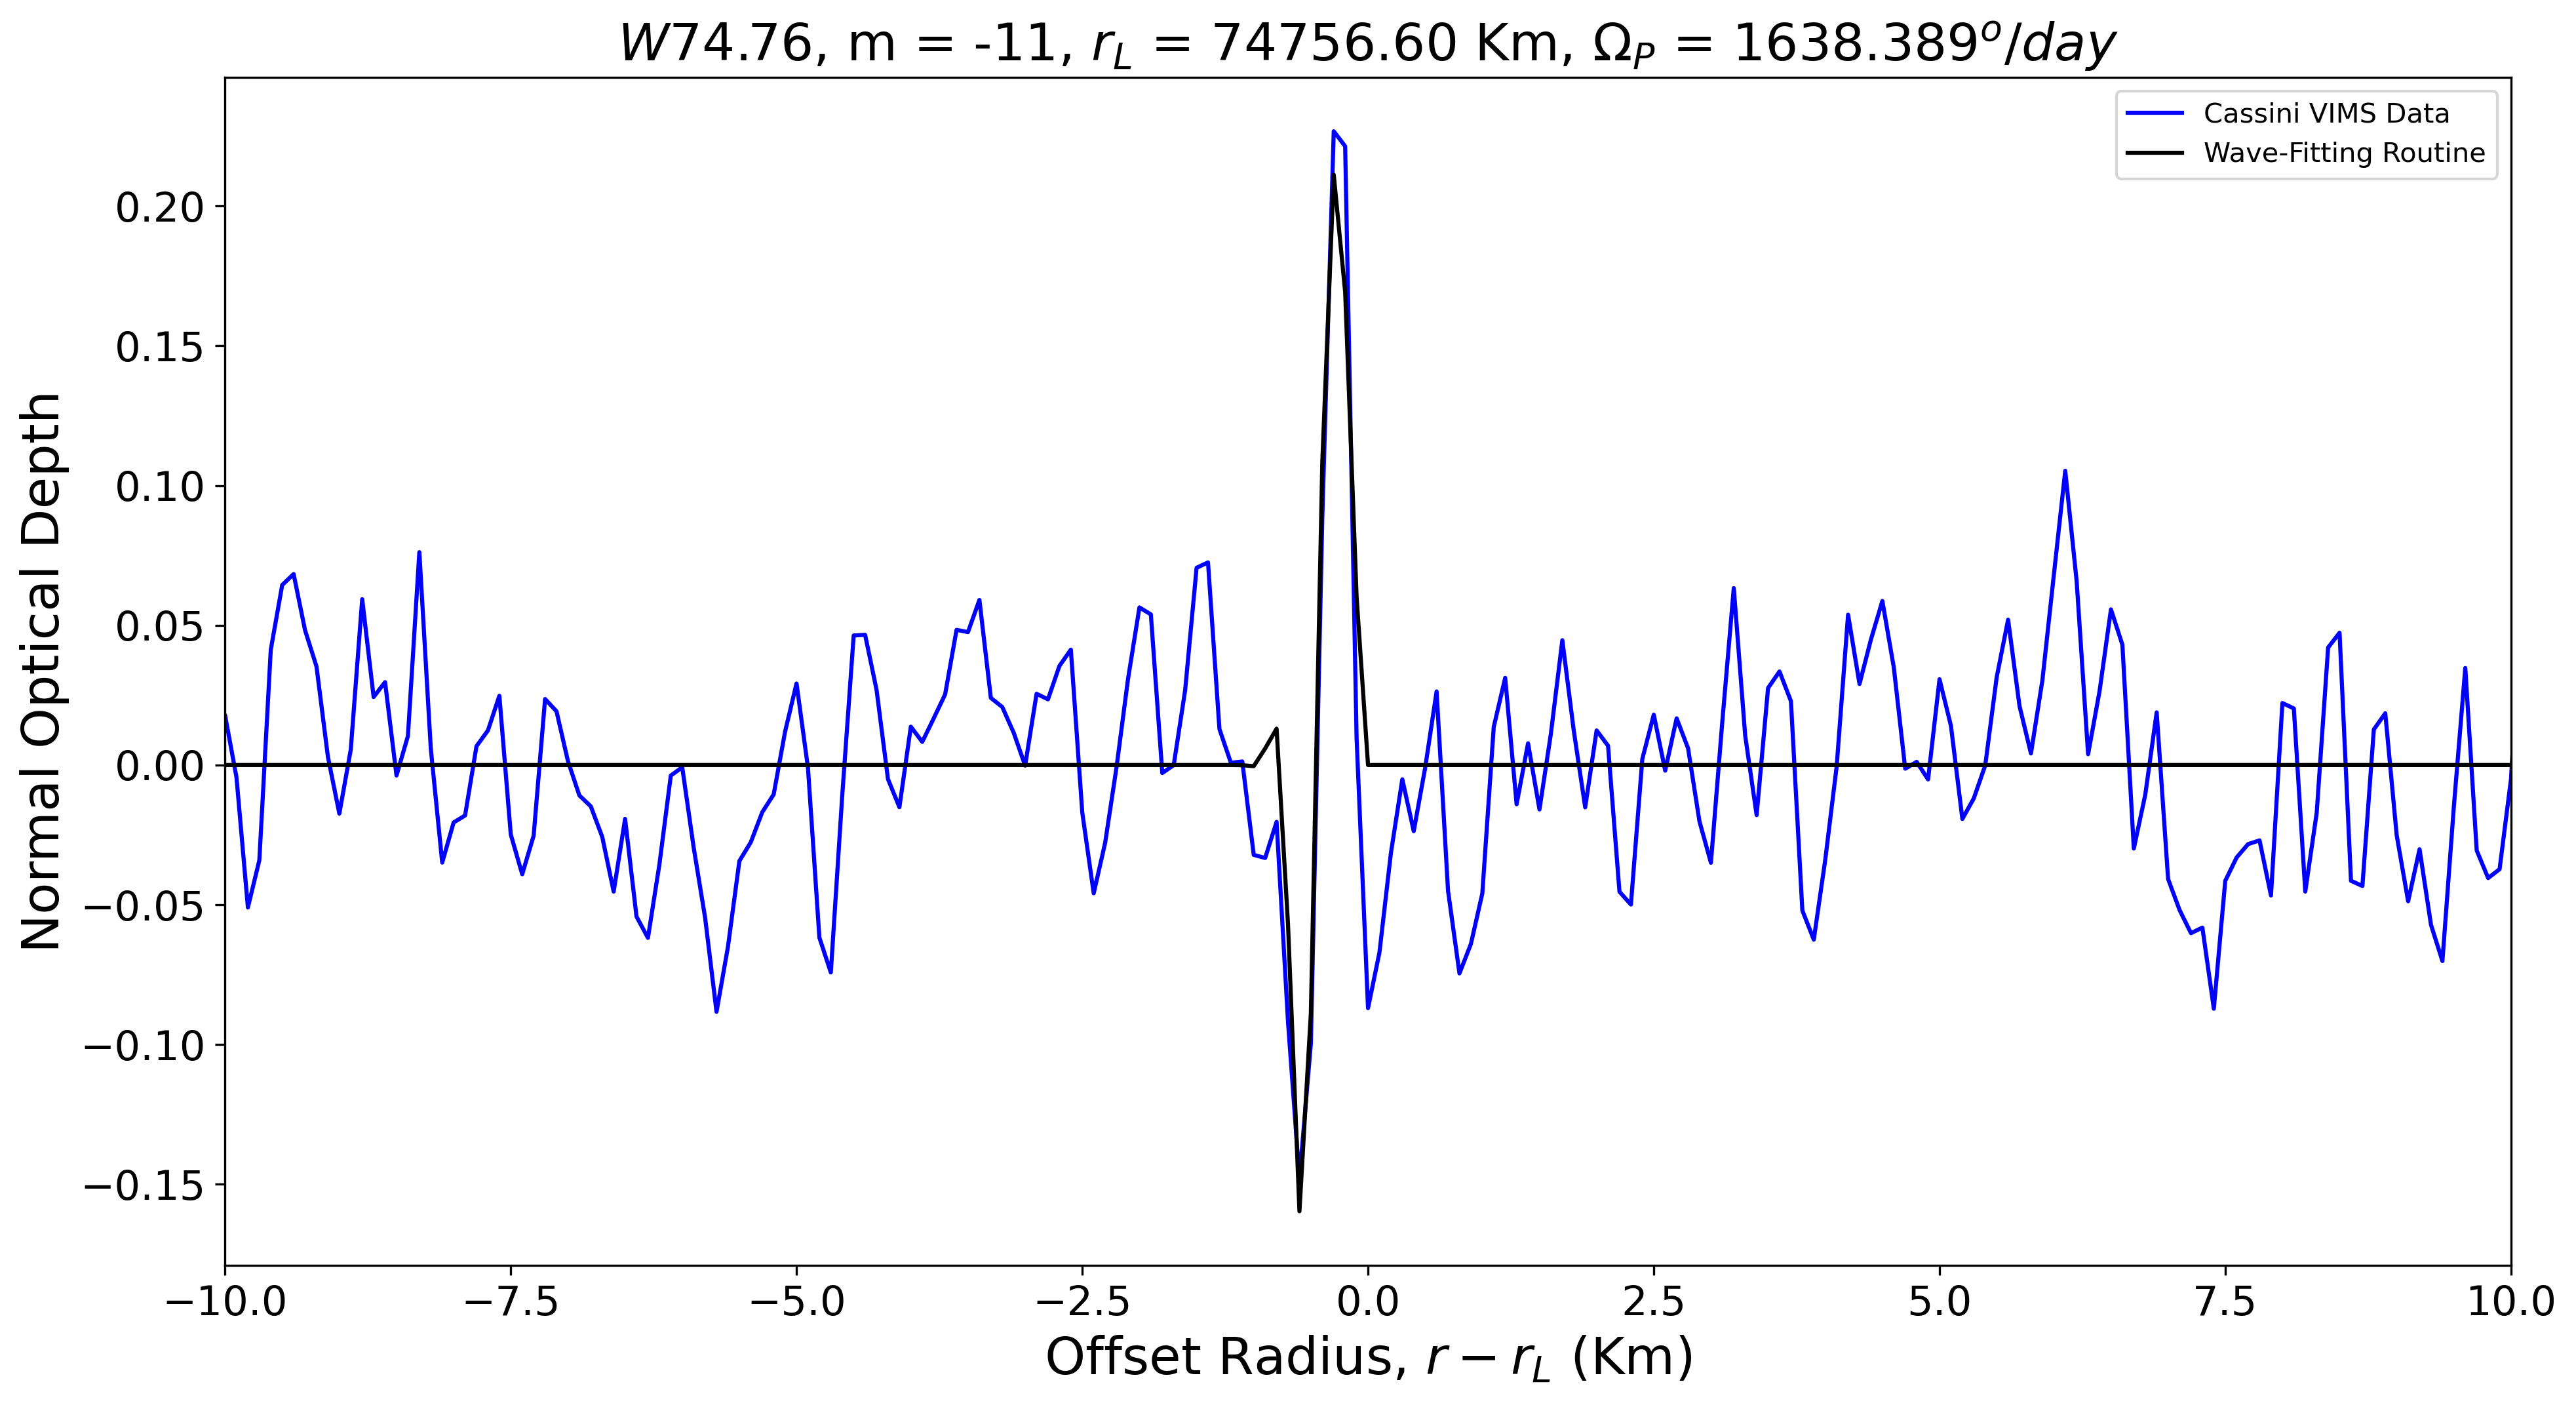
\includegraphics[width=0.3\textwidth, height=0.2\textheight, keepaspectratio]{w7476mp.png}} &
        \subcaptionbox{W75.14}{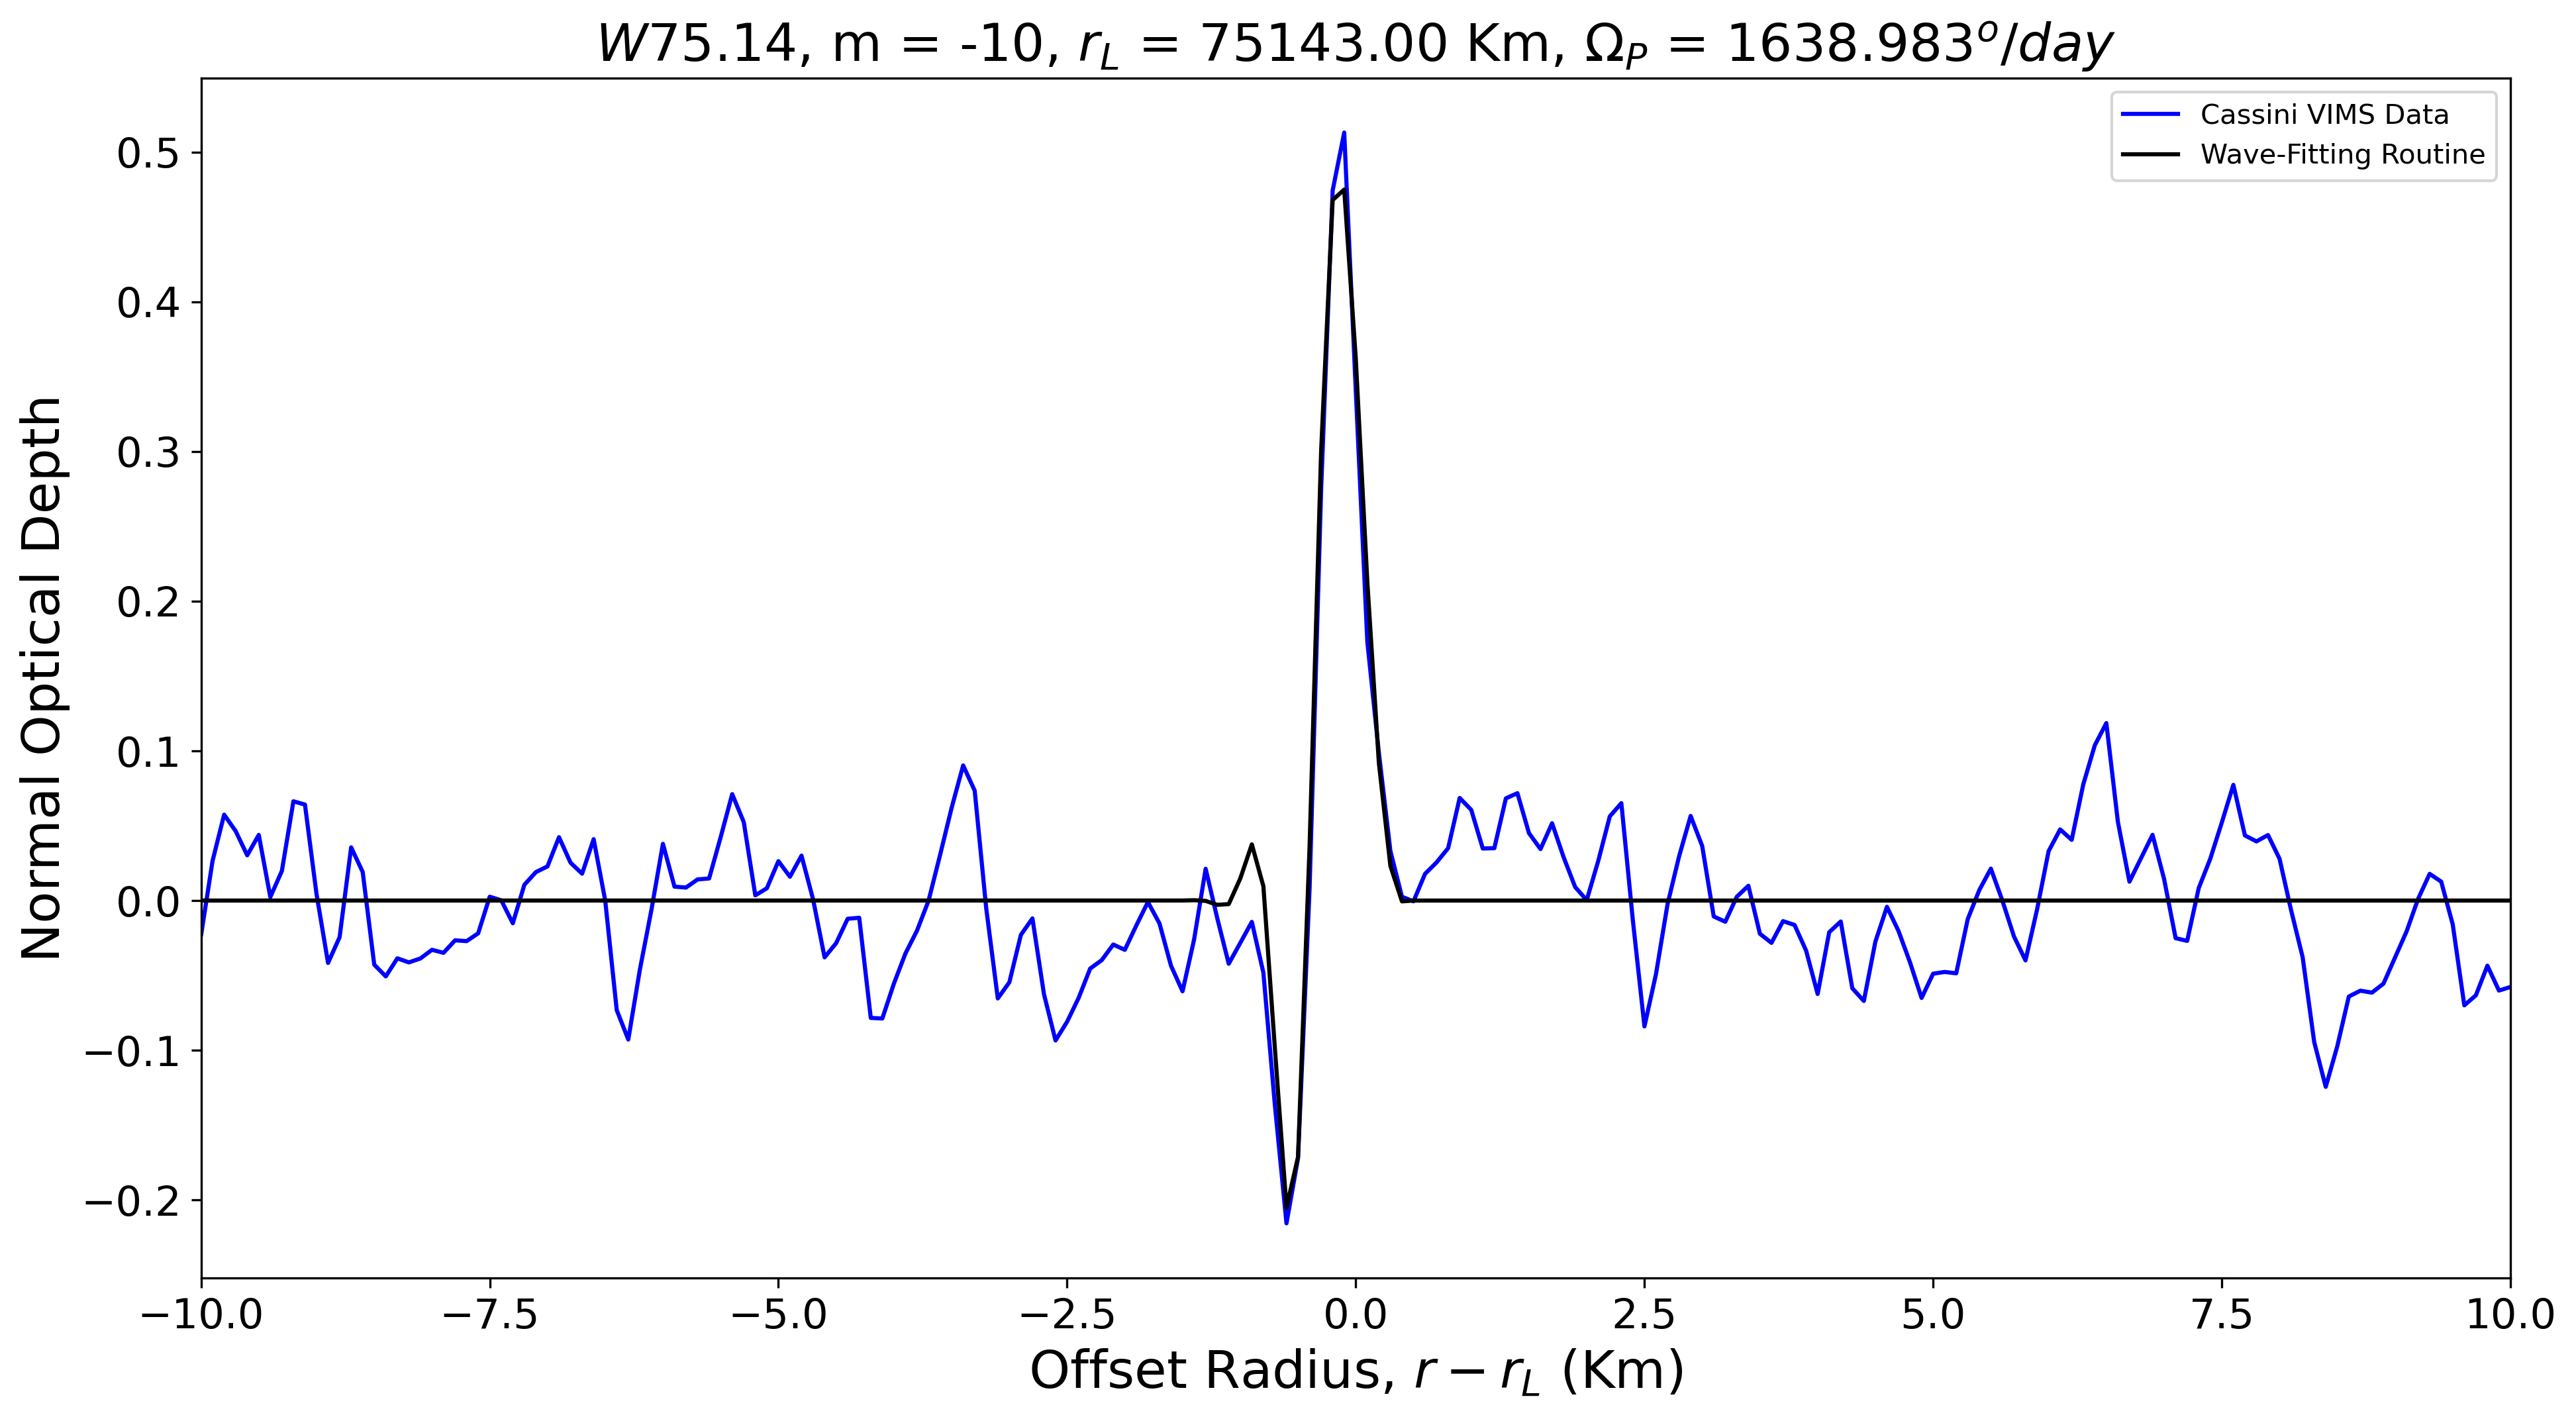
\includegraphics[width=0.3\textwidth, height=0.2\textheight, keepaspectratio]{w7514mp.png}} &
        \subcaptionbox{W76.02A}{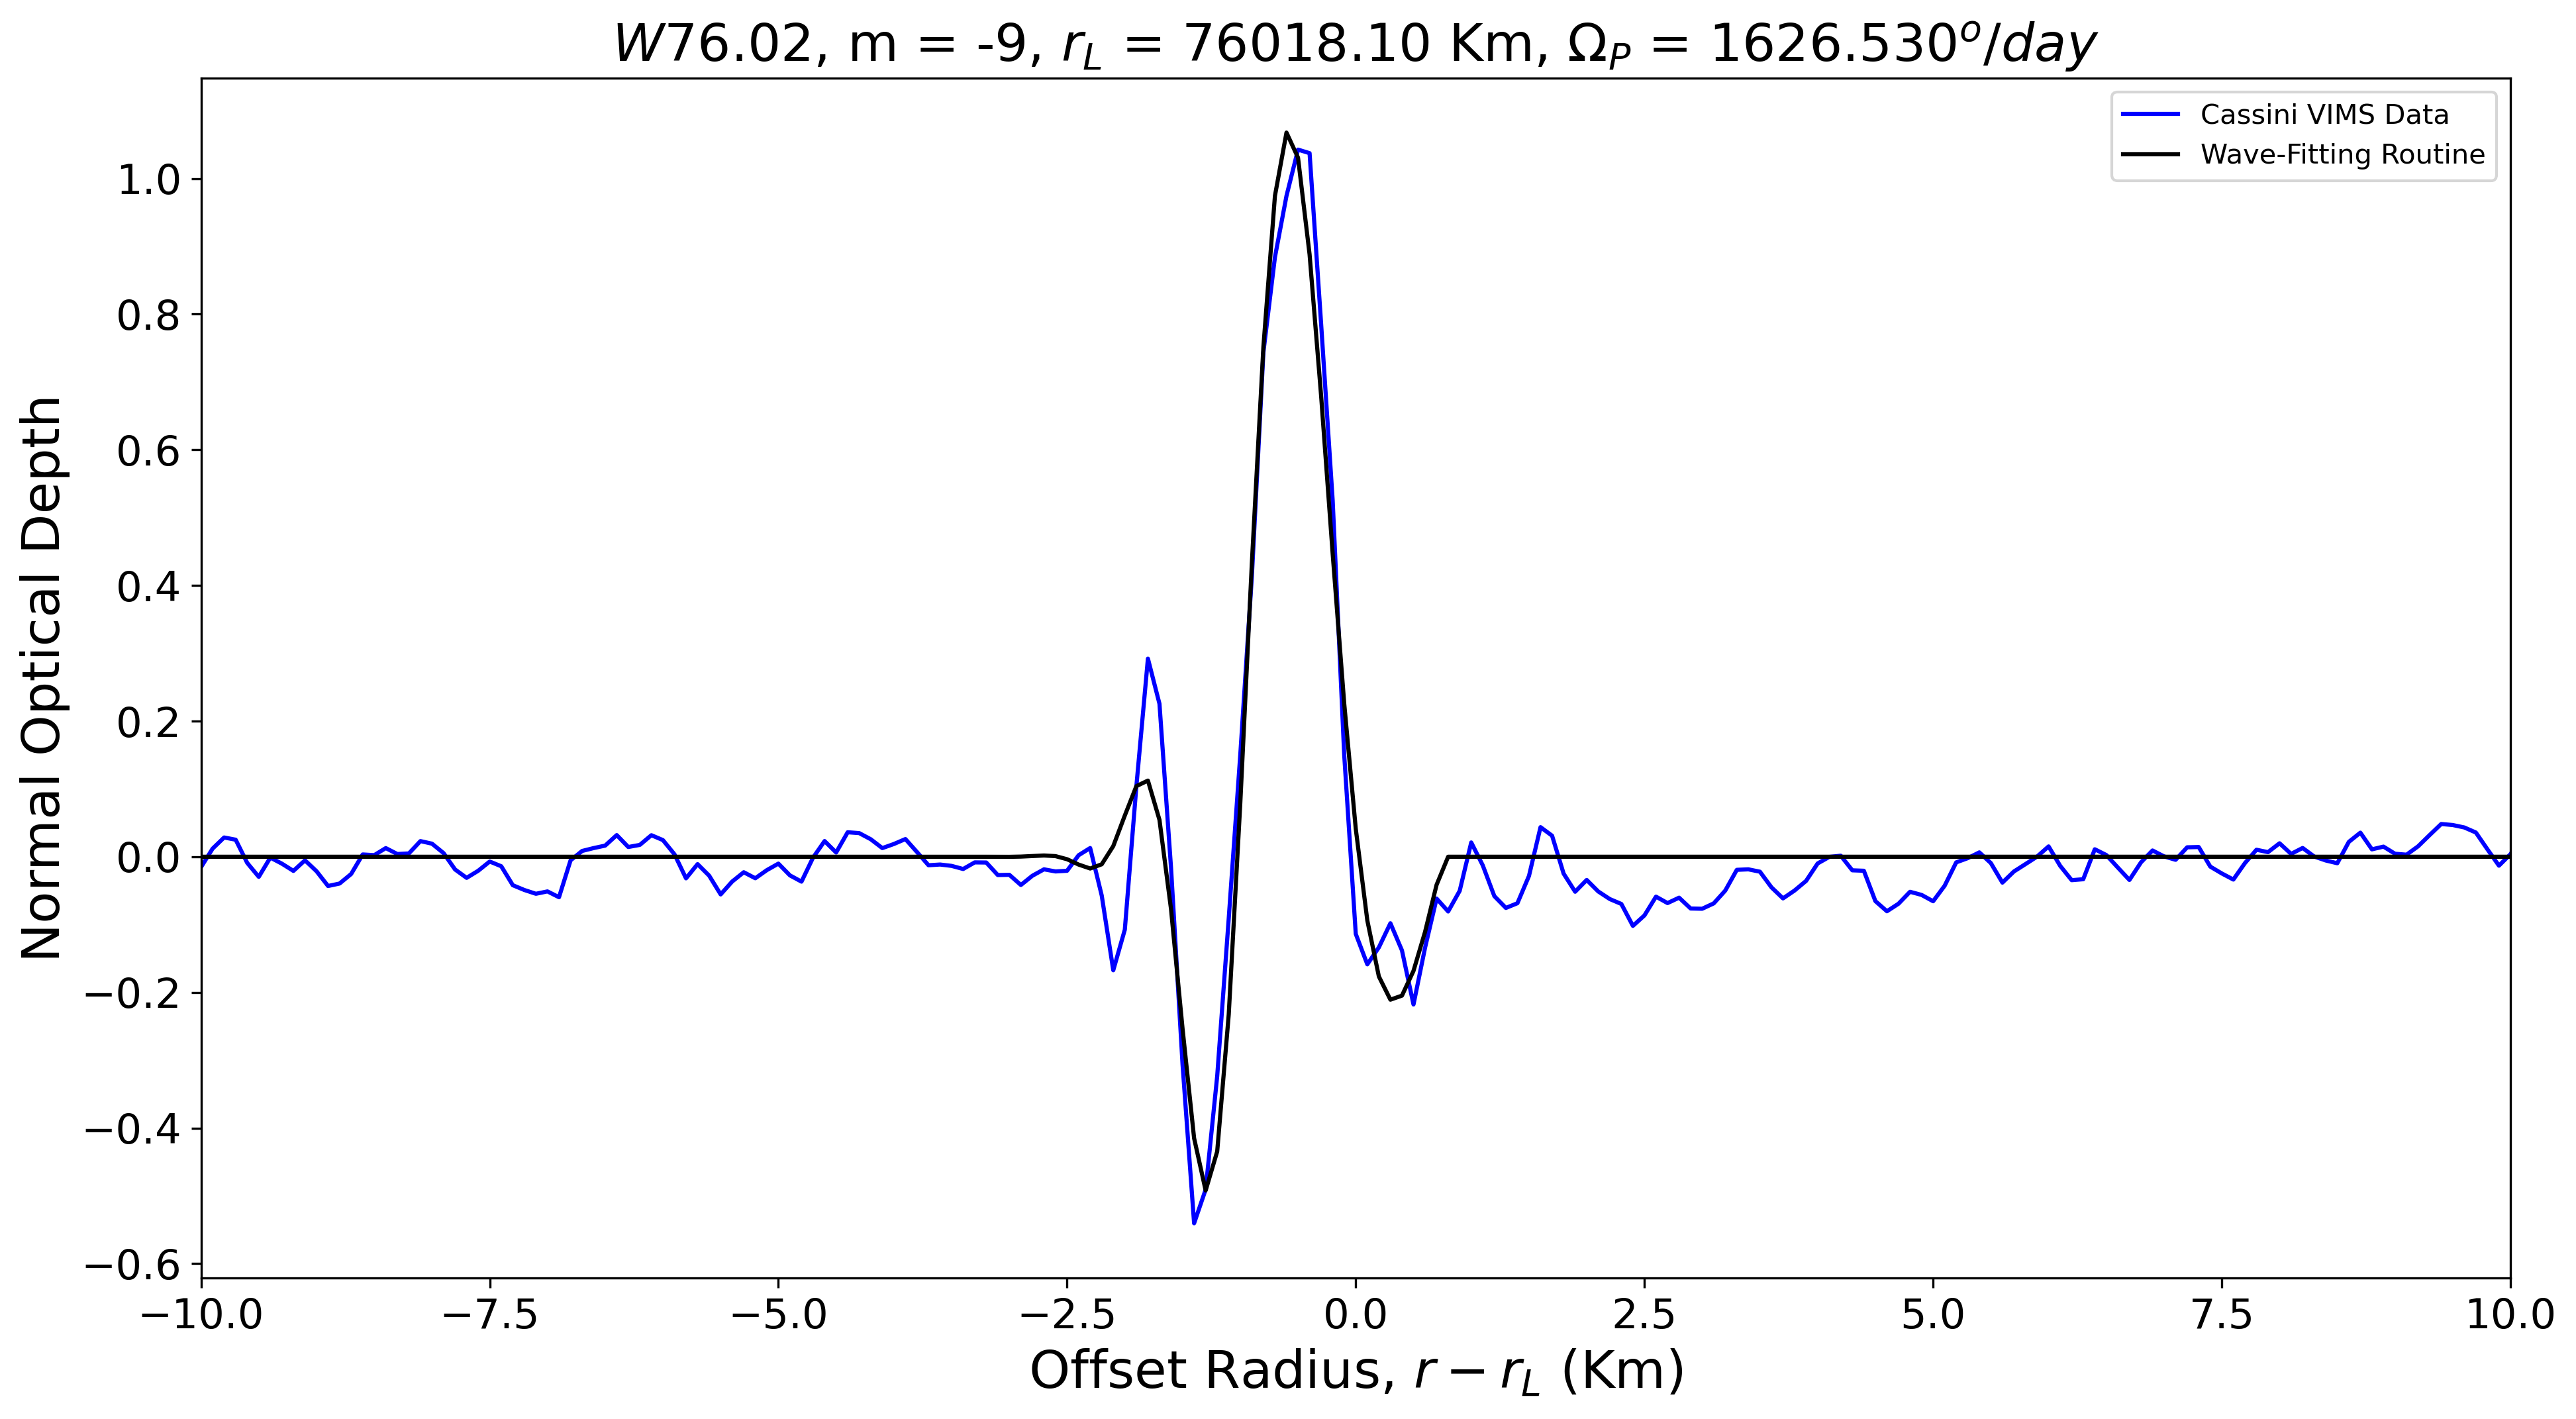
\includegraphics[width=0.3\textwidth, height=0.2\textheight, keepaspectratio]{w7602mp.png}} \\
        \subcaptionbox{W76.44}{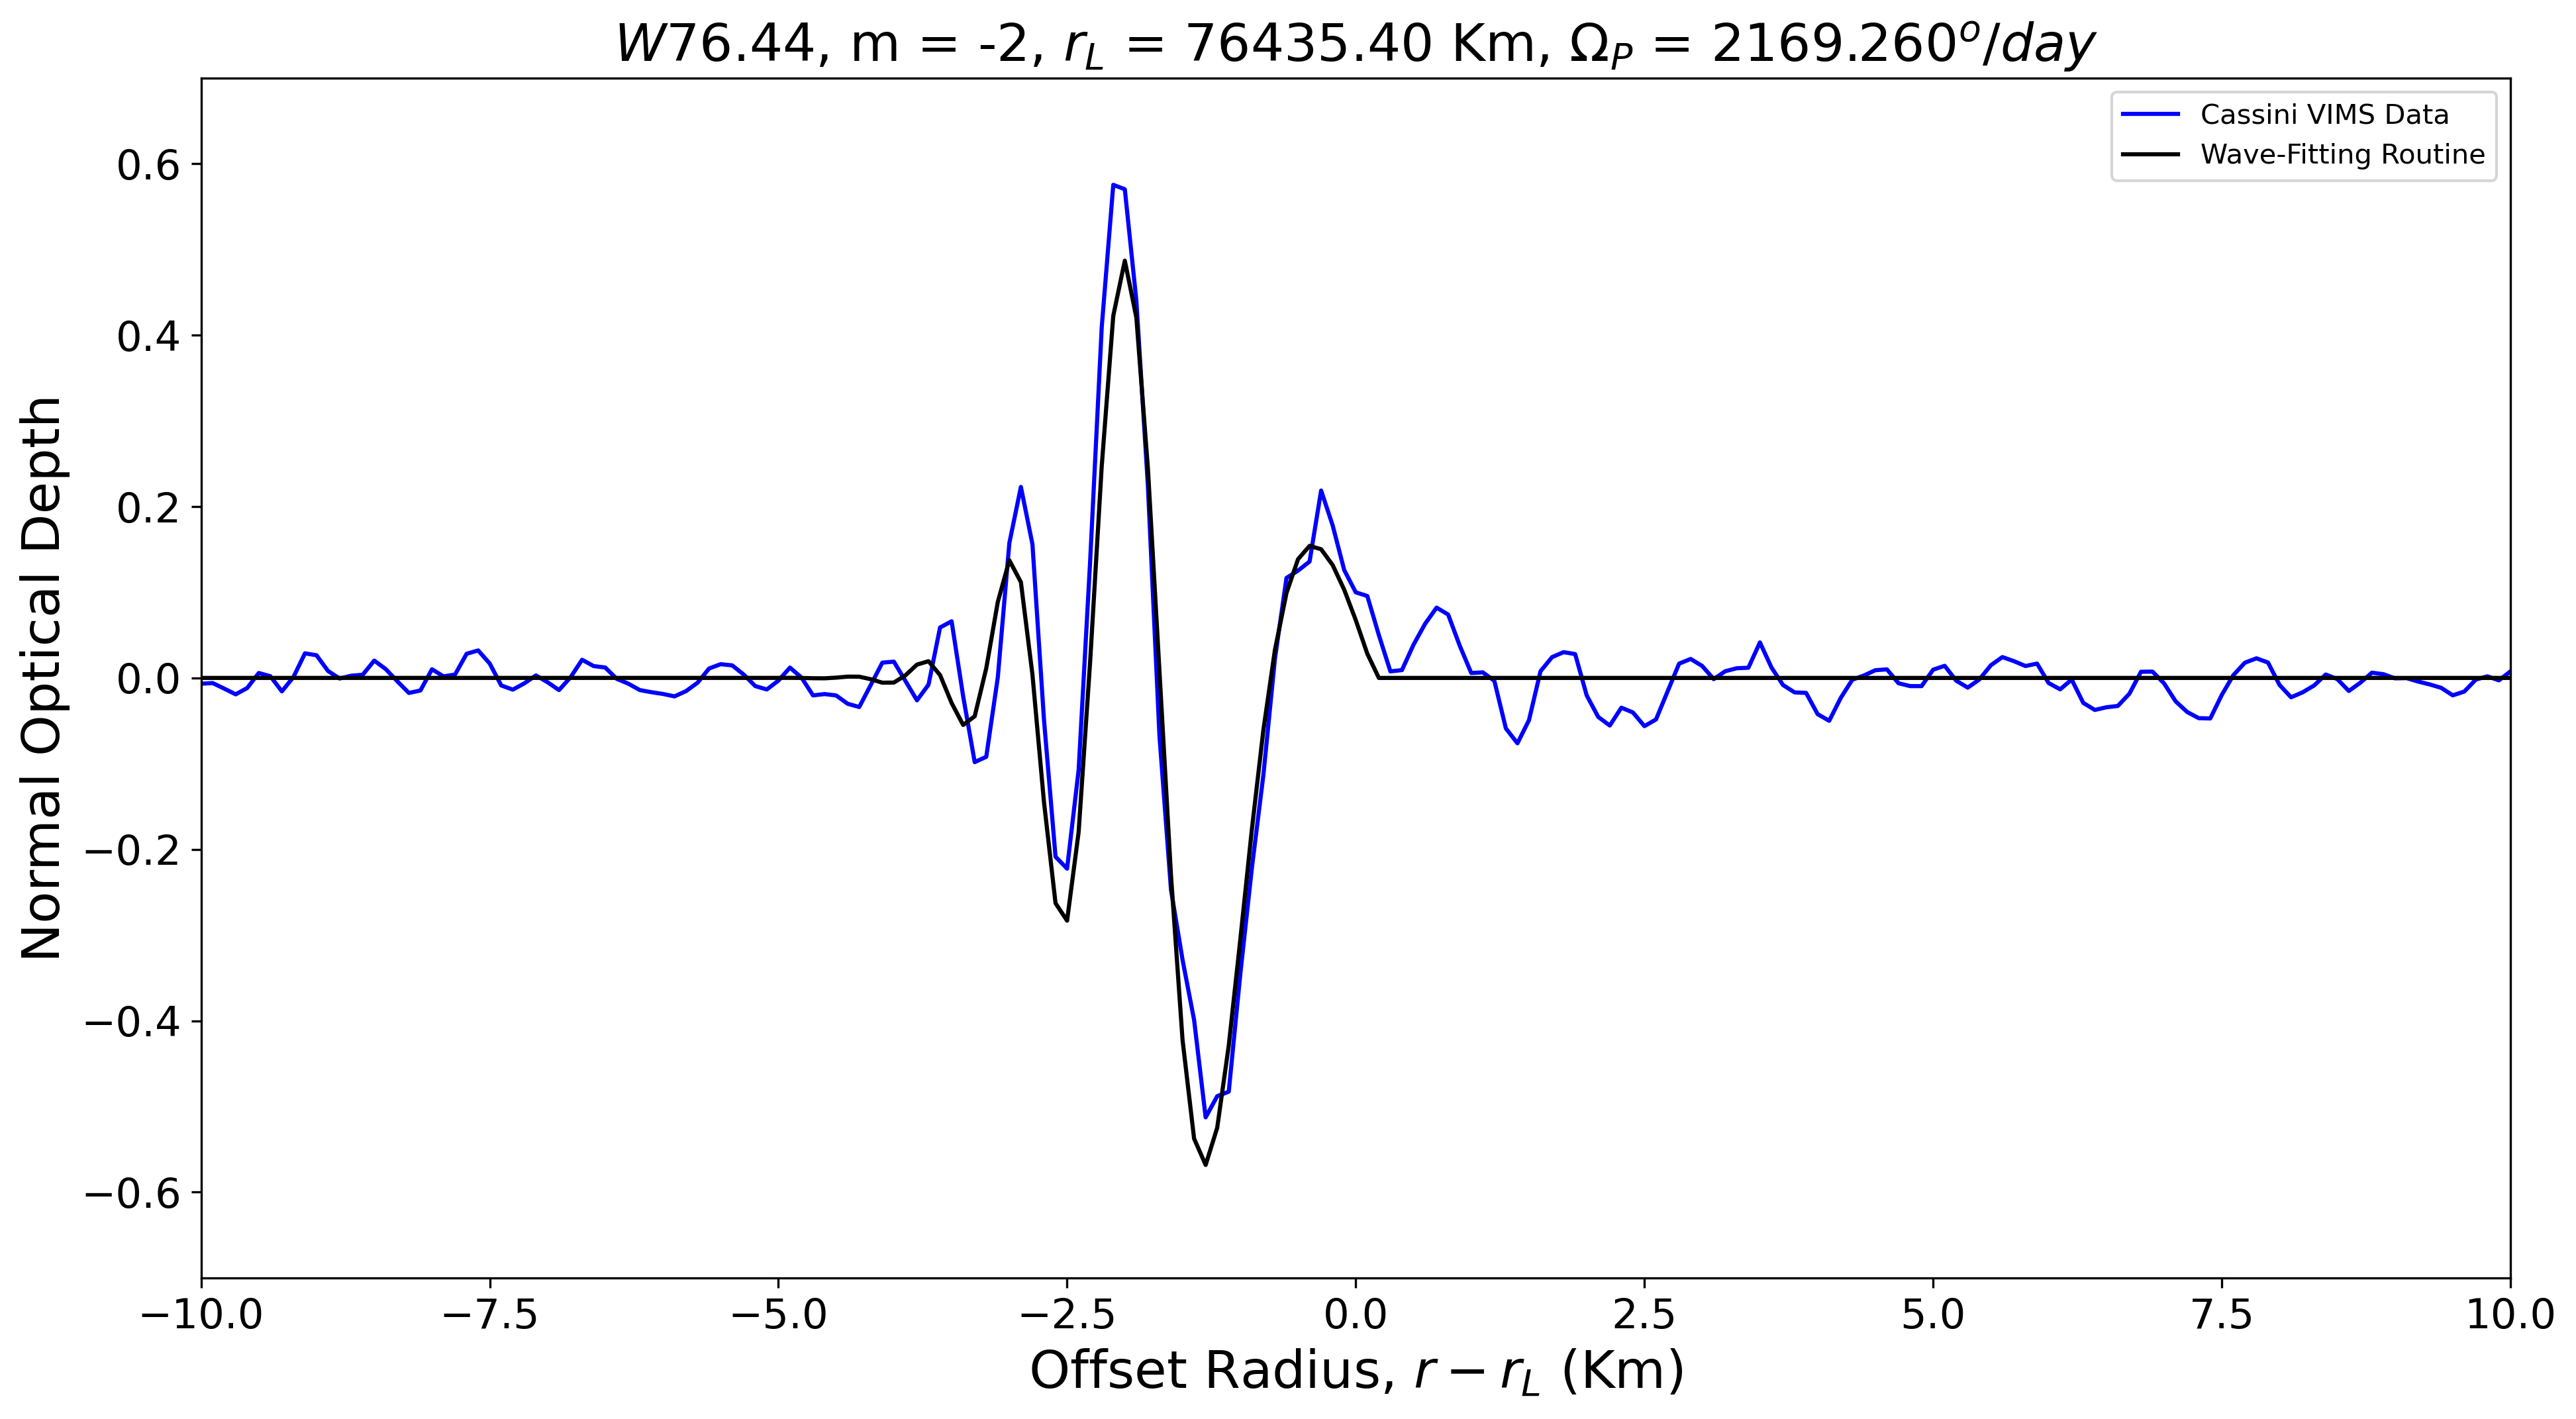
\includegraphics[width=0.3\textwidth, height=0.2\textheight, keepaspectratio]{w7644mp.png}} &
        \subcaptionbox{$W76.46^{av}$}{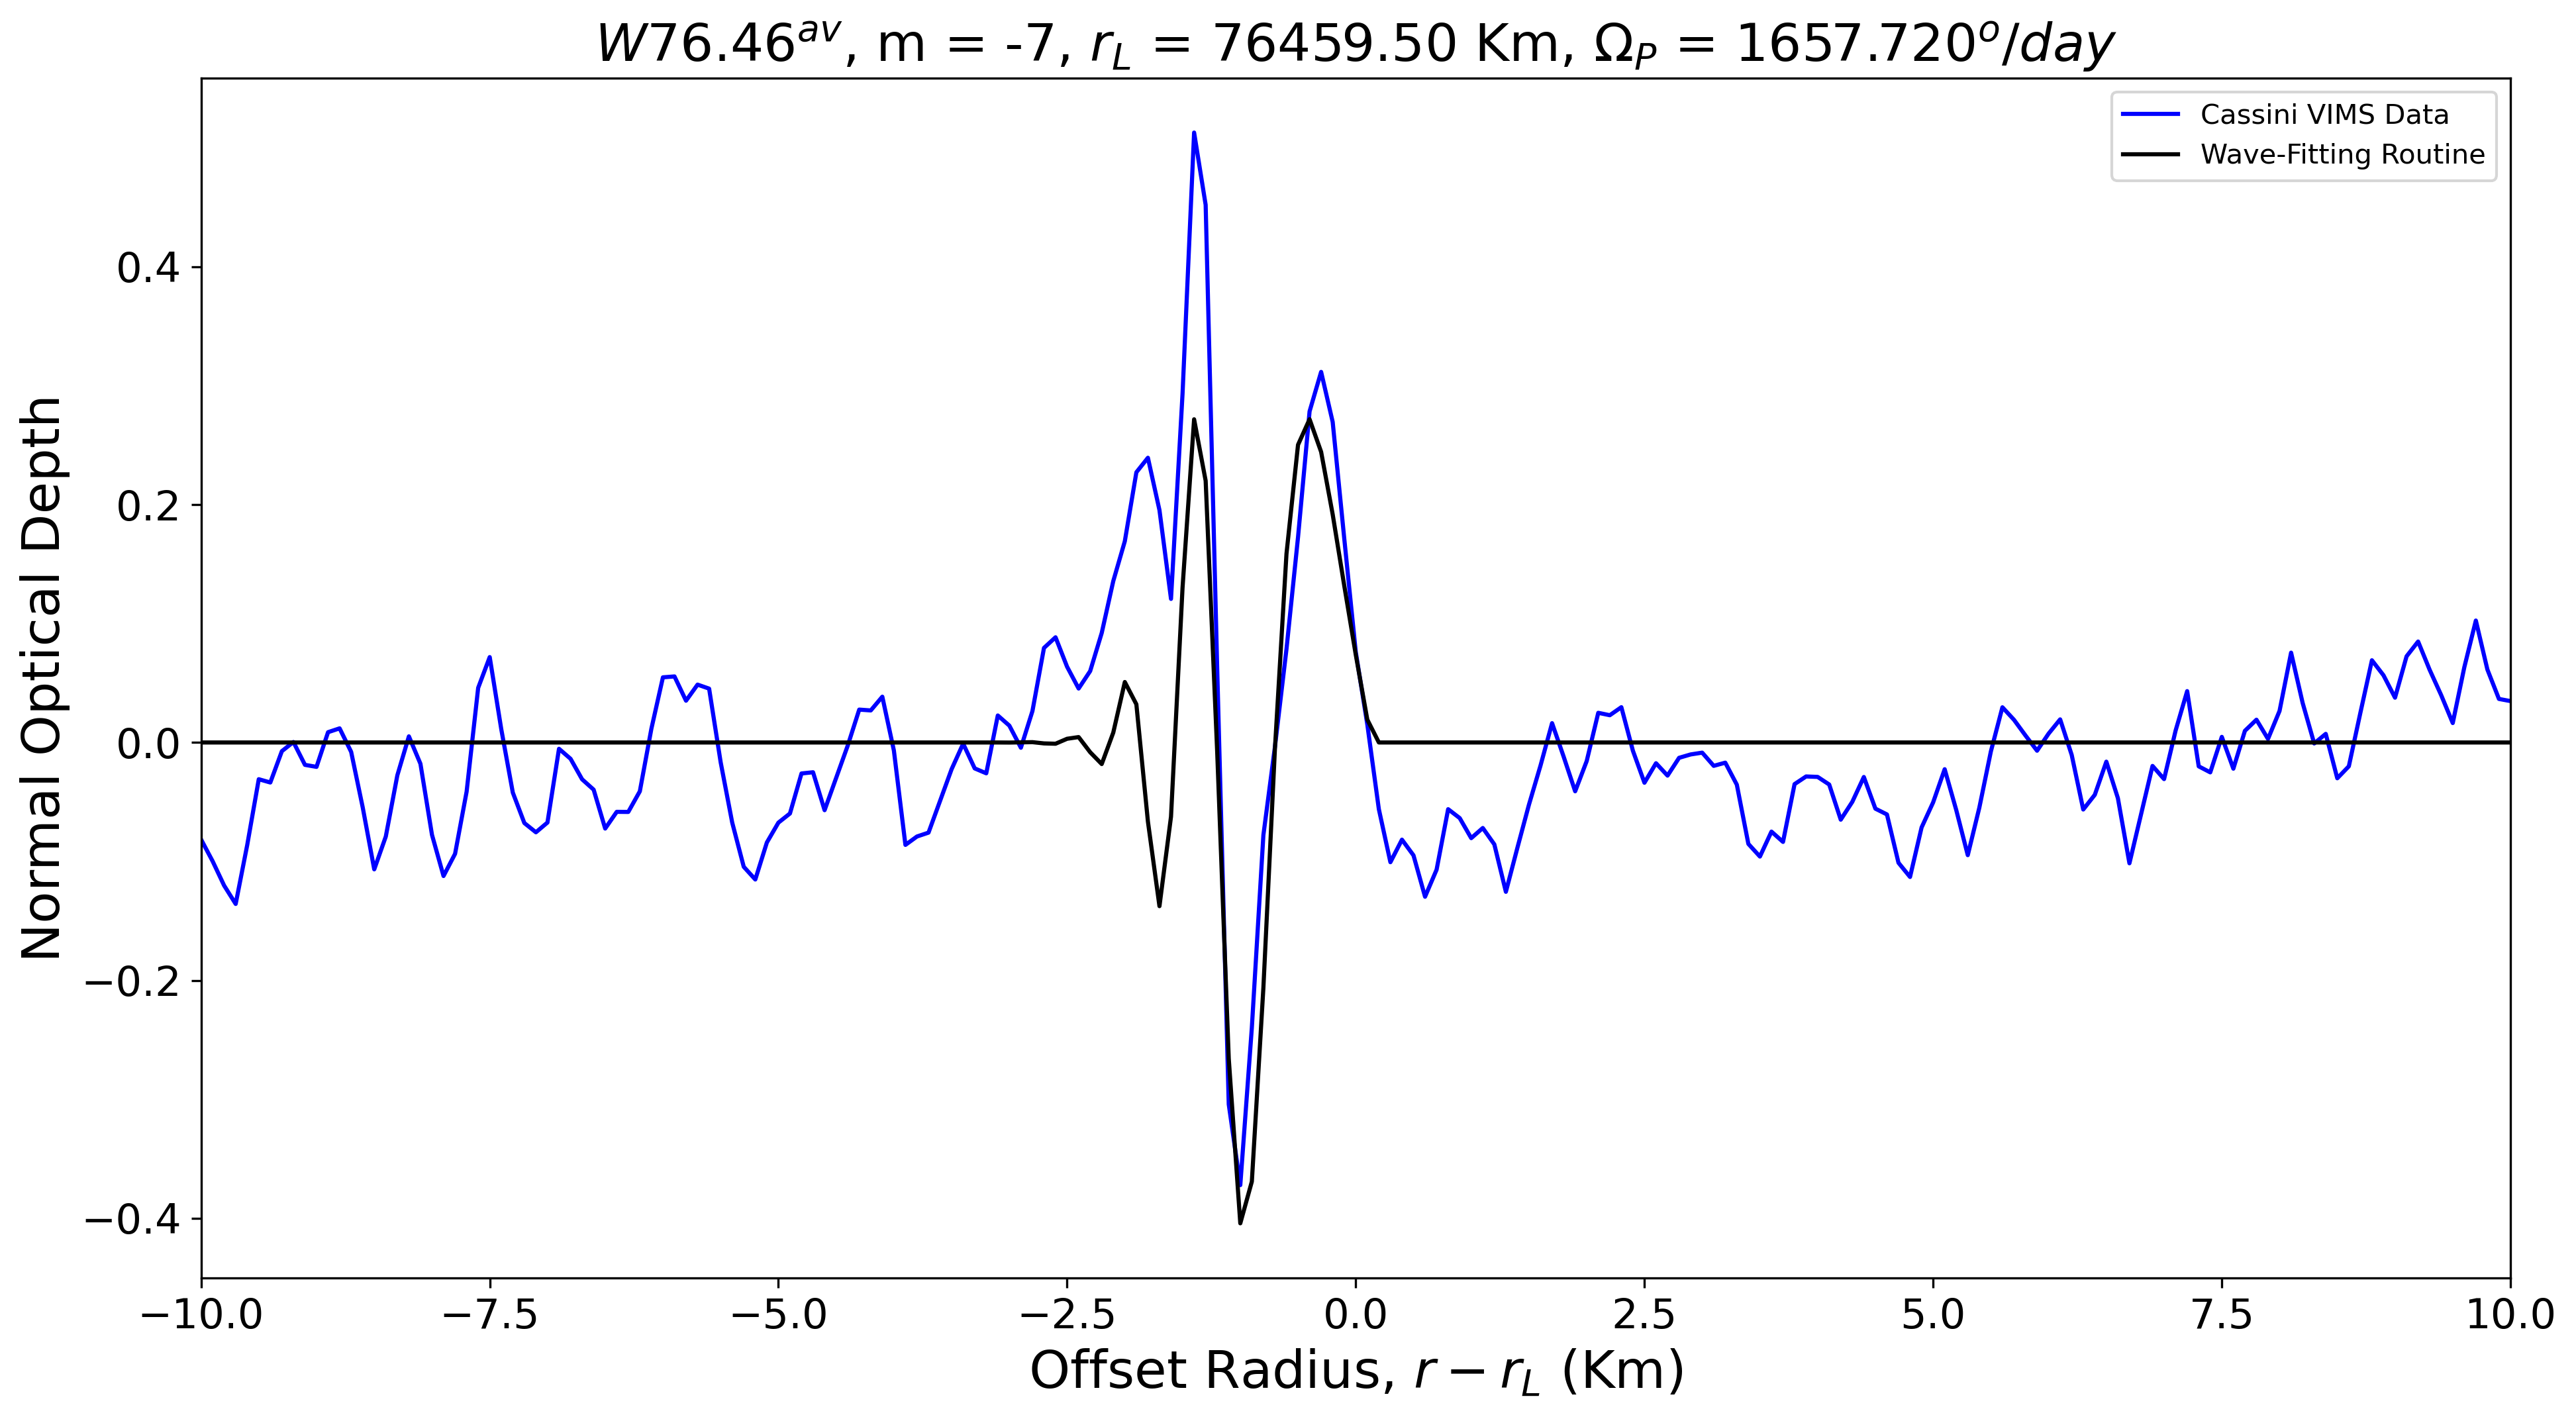
\includegraphics[width=0.3\textwidth, height=0.2\textheight, keepaspectratio]{w7646avmp.png}} &
        \subcaptionbox{W77.34}{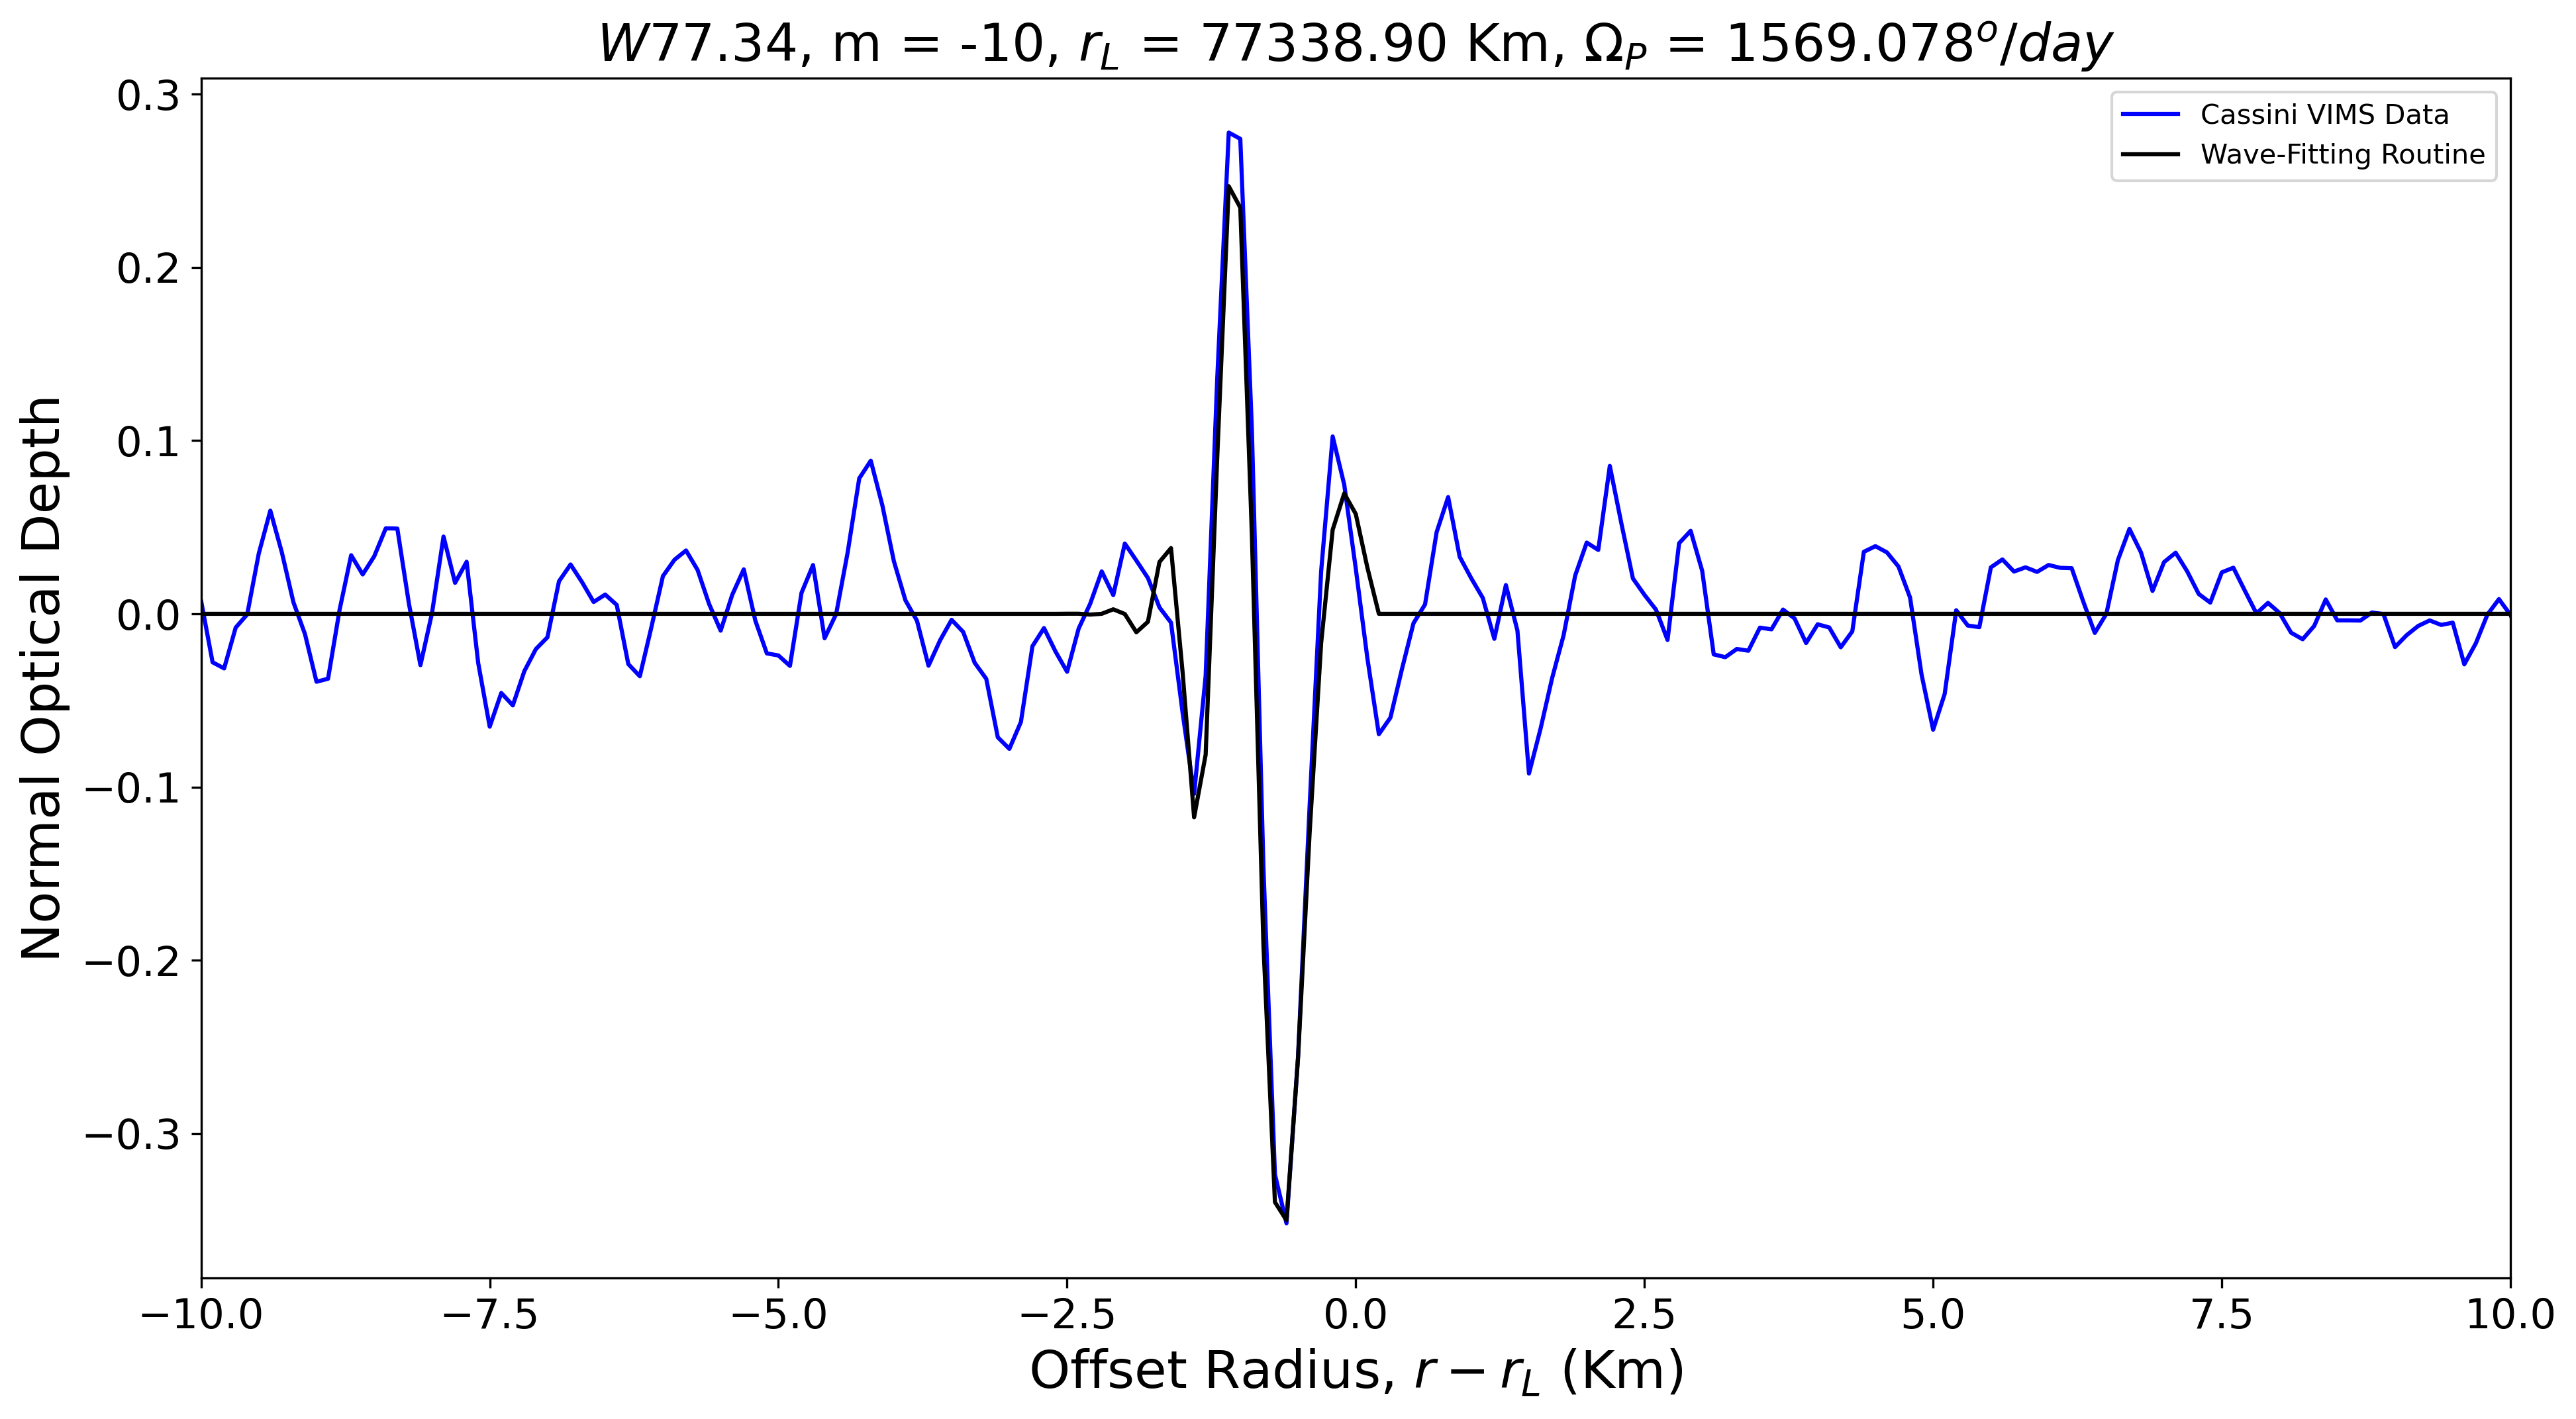
\includegraphics[width=0.3\textwidth, height=0.2\textheight, keepaspectratio]{w7734mp.png}} \\
        \subcaptionbox{W78.51}{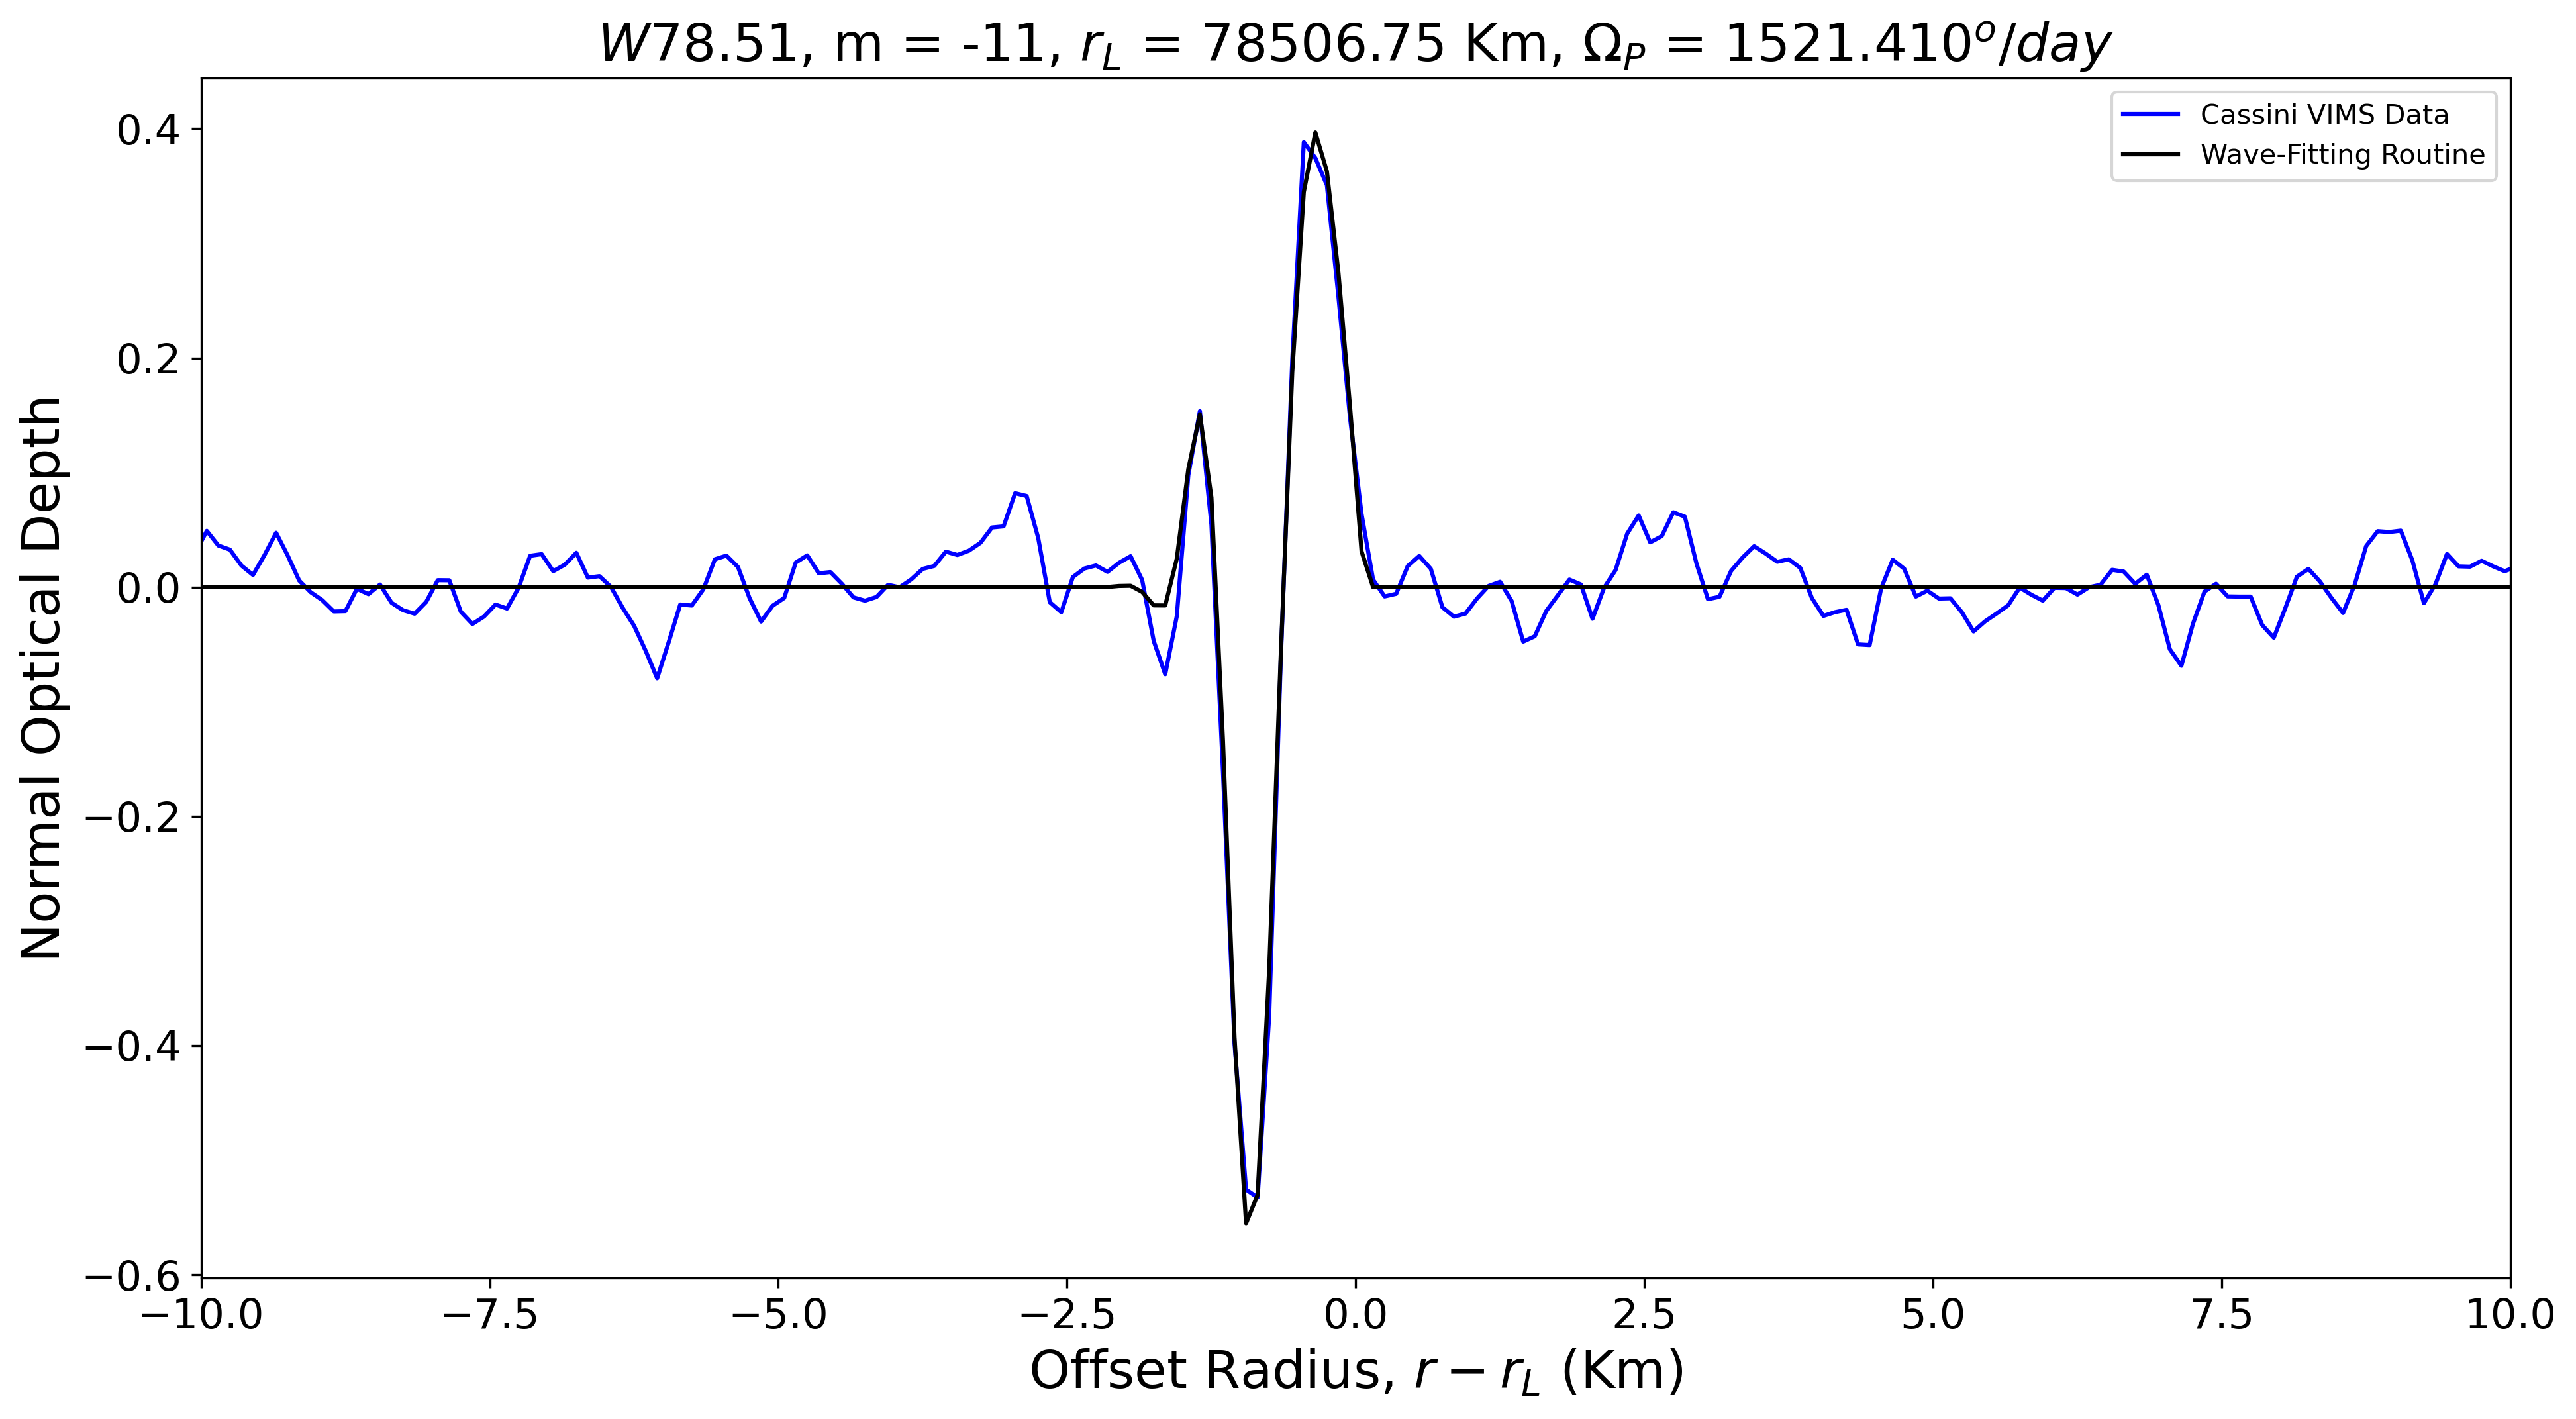
\includegraphics[width=0.3\textwidth, height=0.2\textheight, keepaspectratio]{w7851mp.png}} &
        \subcaptionbox{W79.04}{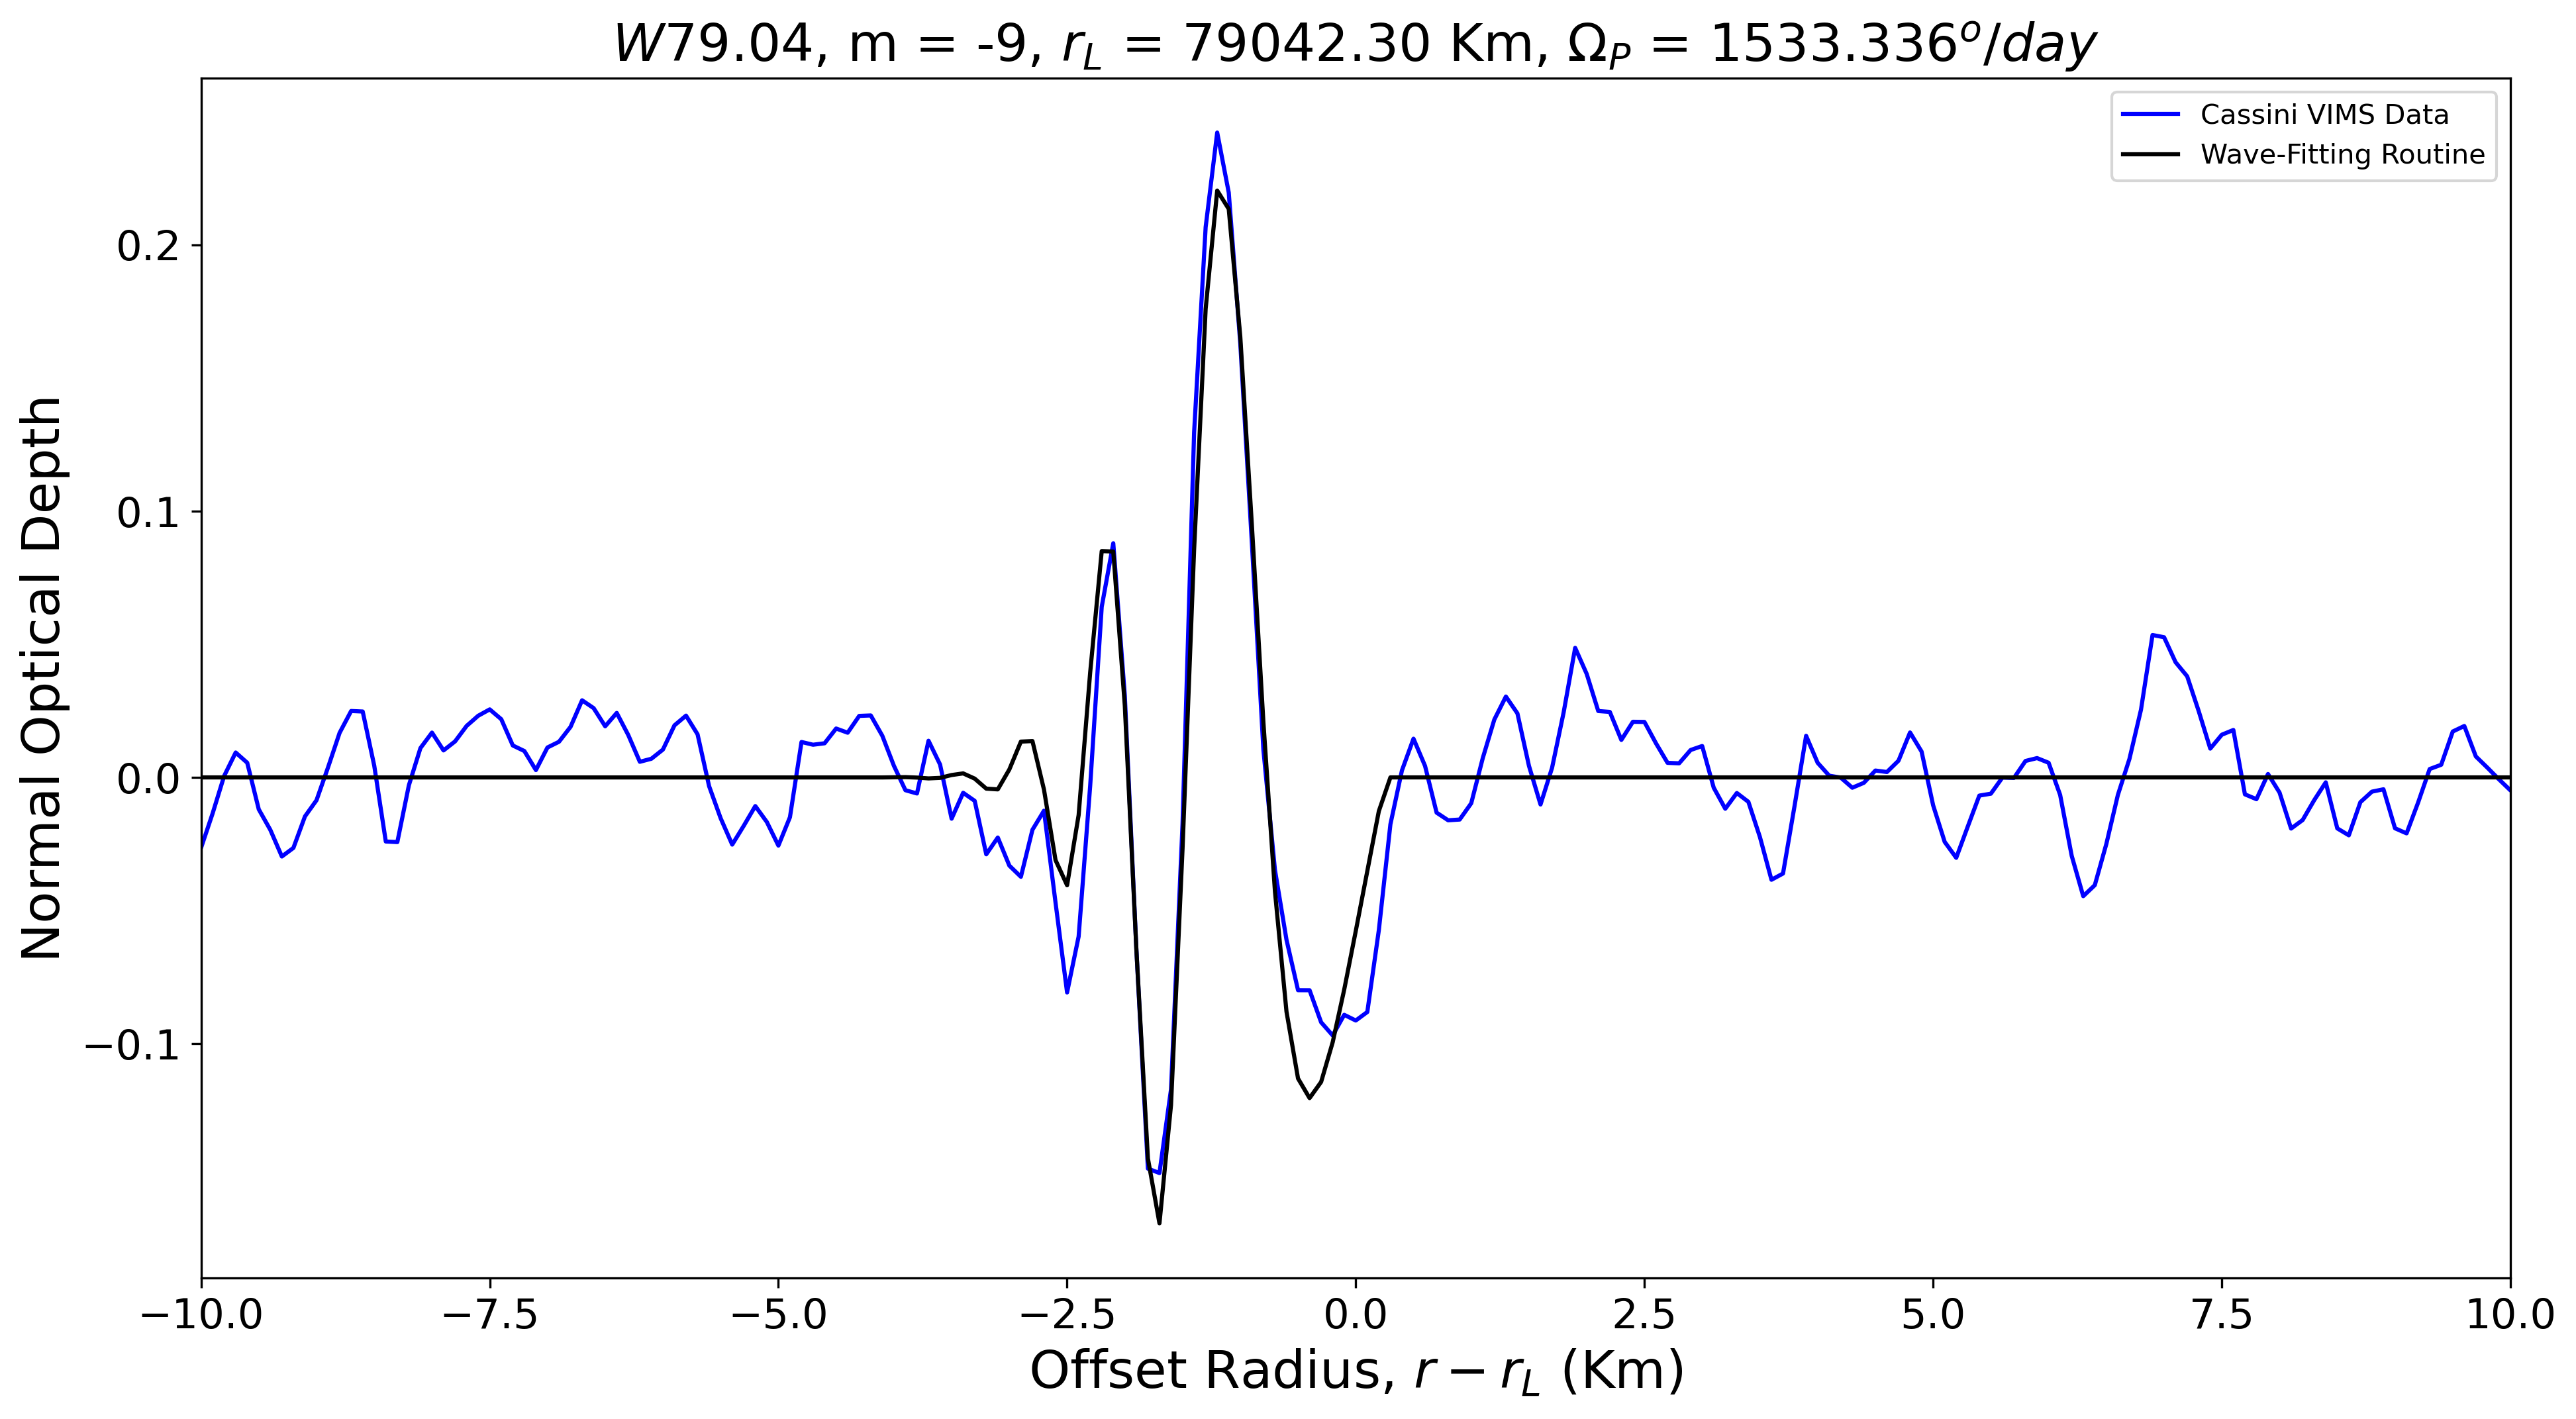
\includegraphics[width=0.3\textwidth, height=0.2\textheight, keepaspectratio]{w7904mp.png}} &
        \subcaptionbox{W79.55}{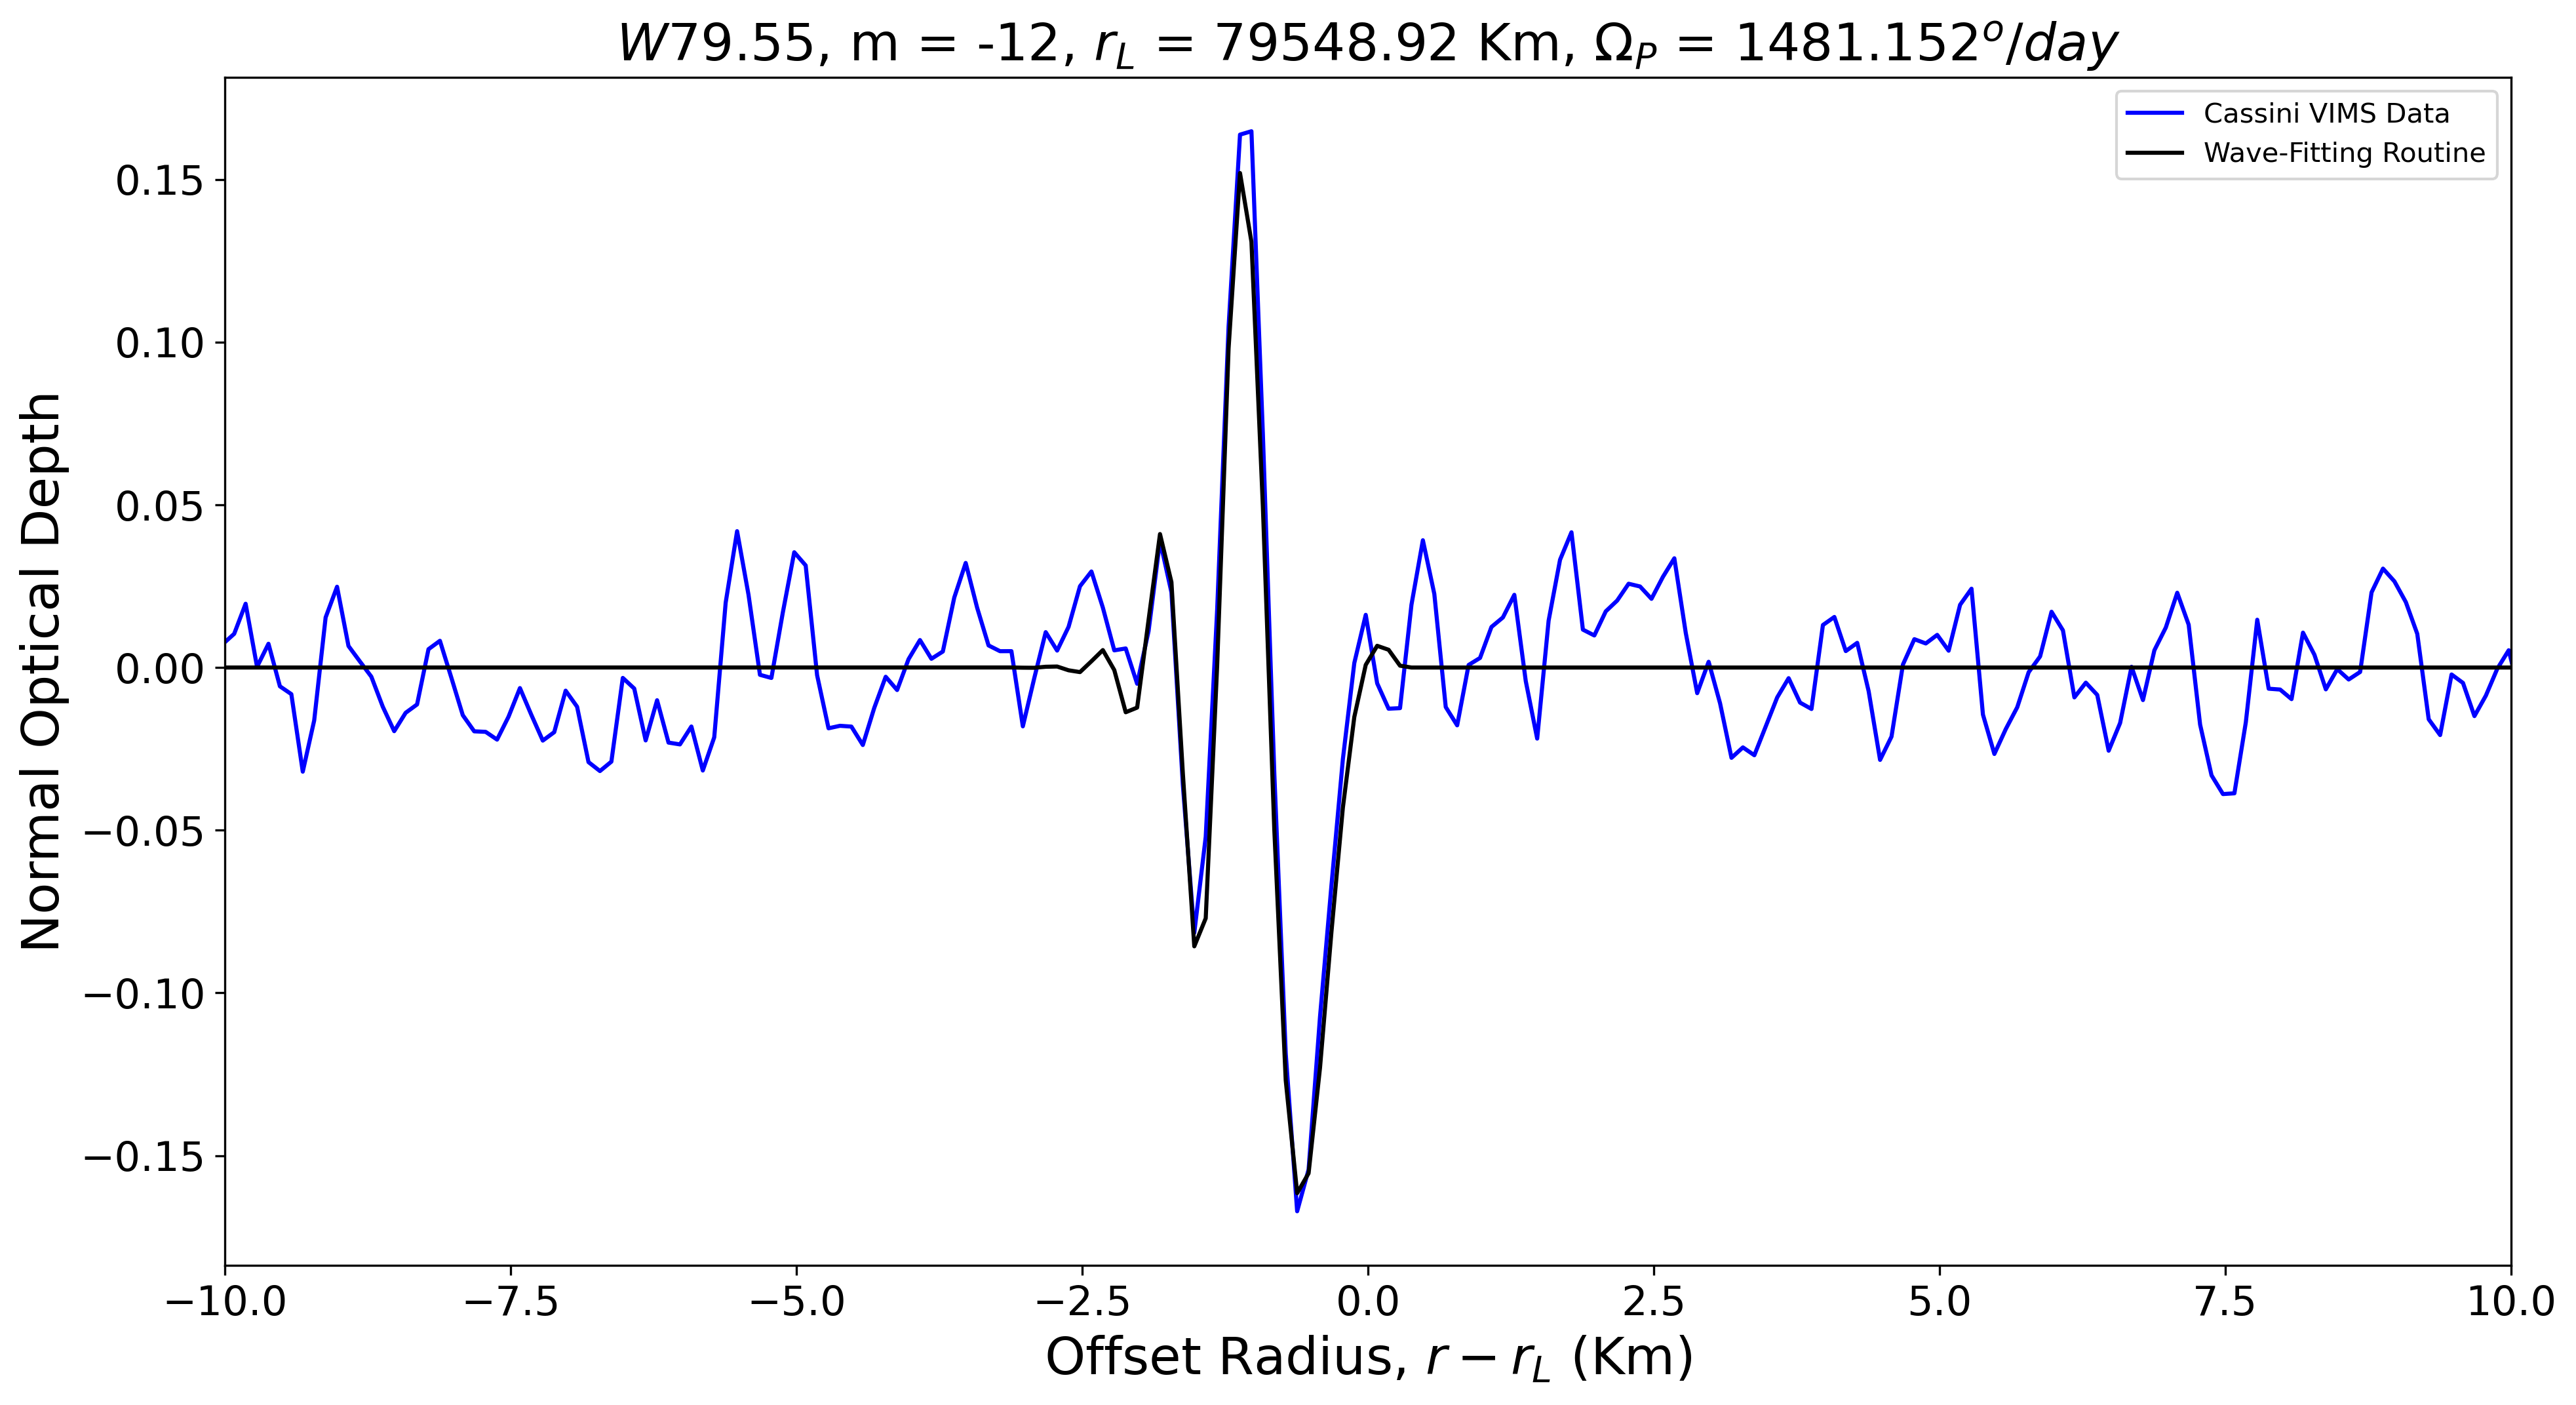
\includegraphics[width=0.3\textwidth, height=0.2\textheight, keepaspectratio]{w7955mp.png}} \\
    \end{tabular}
    \caption{A catalogue of plots from wave-fitting routine exercise for given satellite and planetary resonances.}
\end{figure}

\afterpage{%
    \clearpage% Flush earlier floats (otherwise order might not be correct)
    \begin{figure}
        \centering
        \ContinuedFloat
        \begin{tabular}{ccc}
            \subcaptionbox{W80.49}{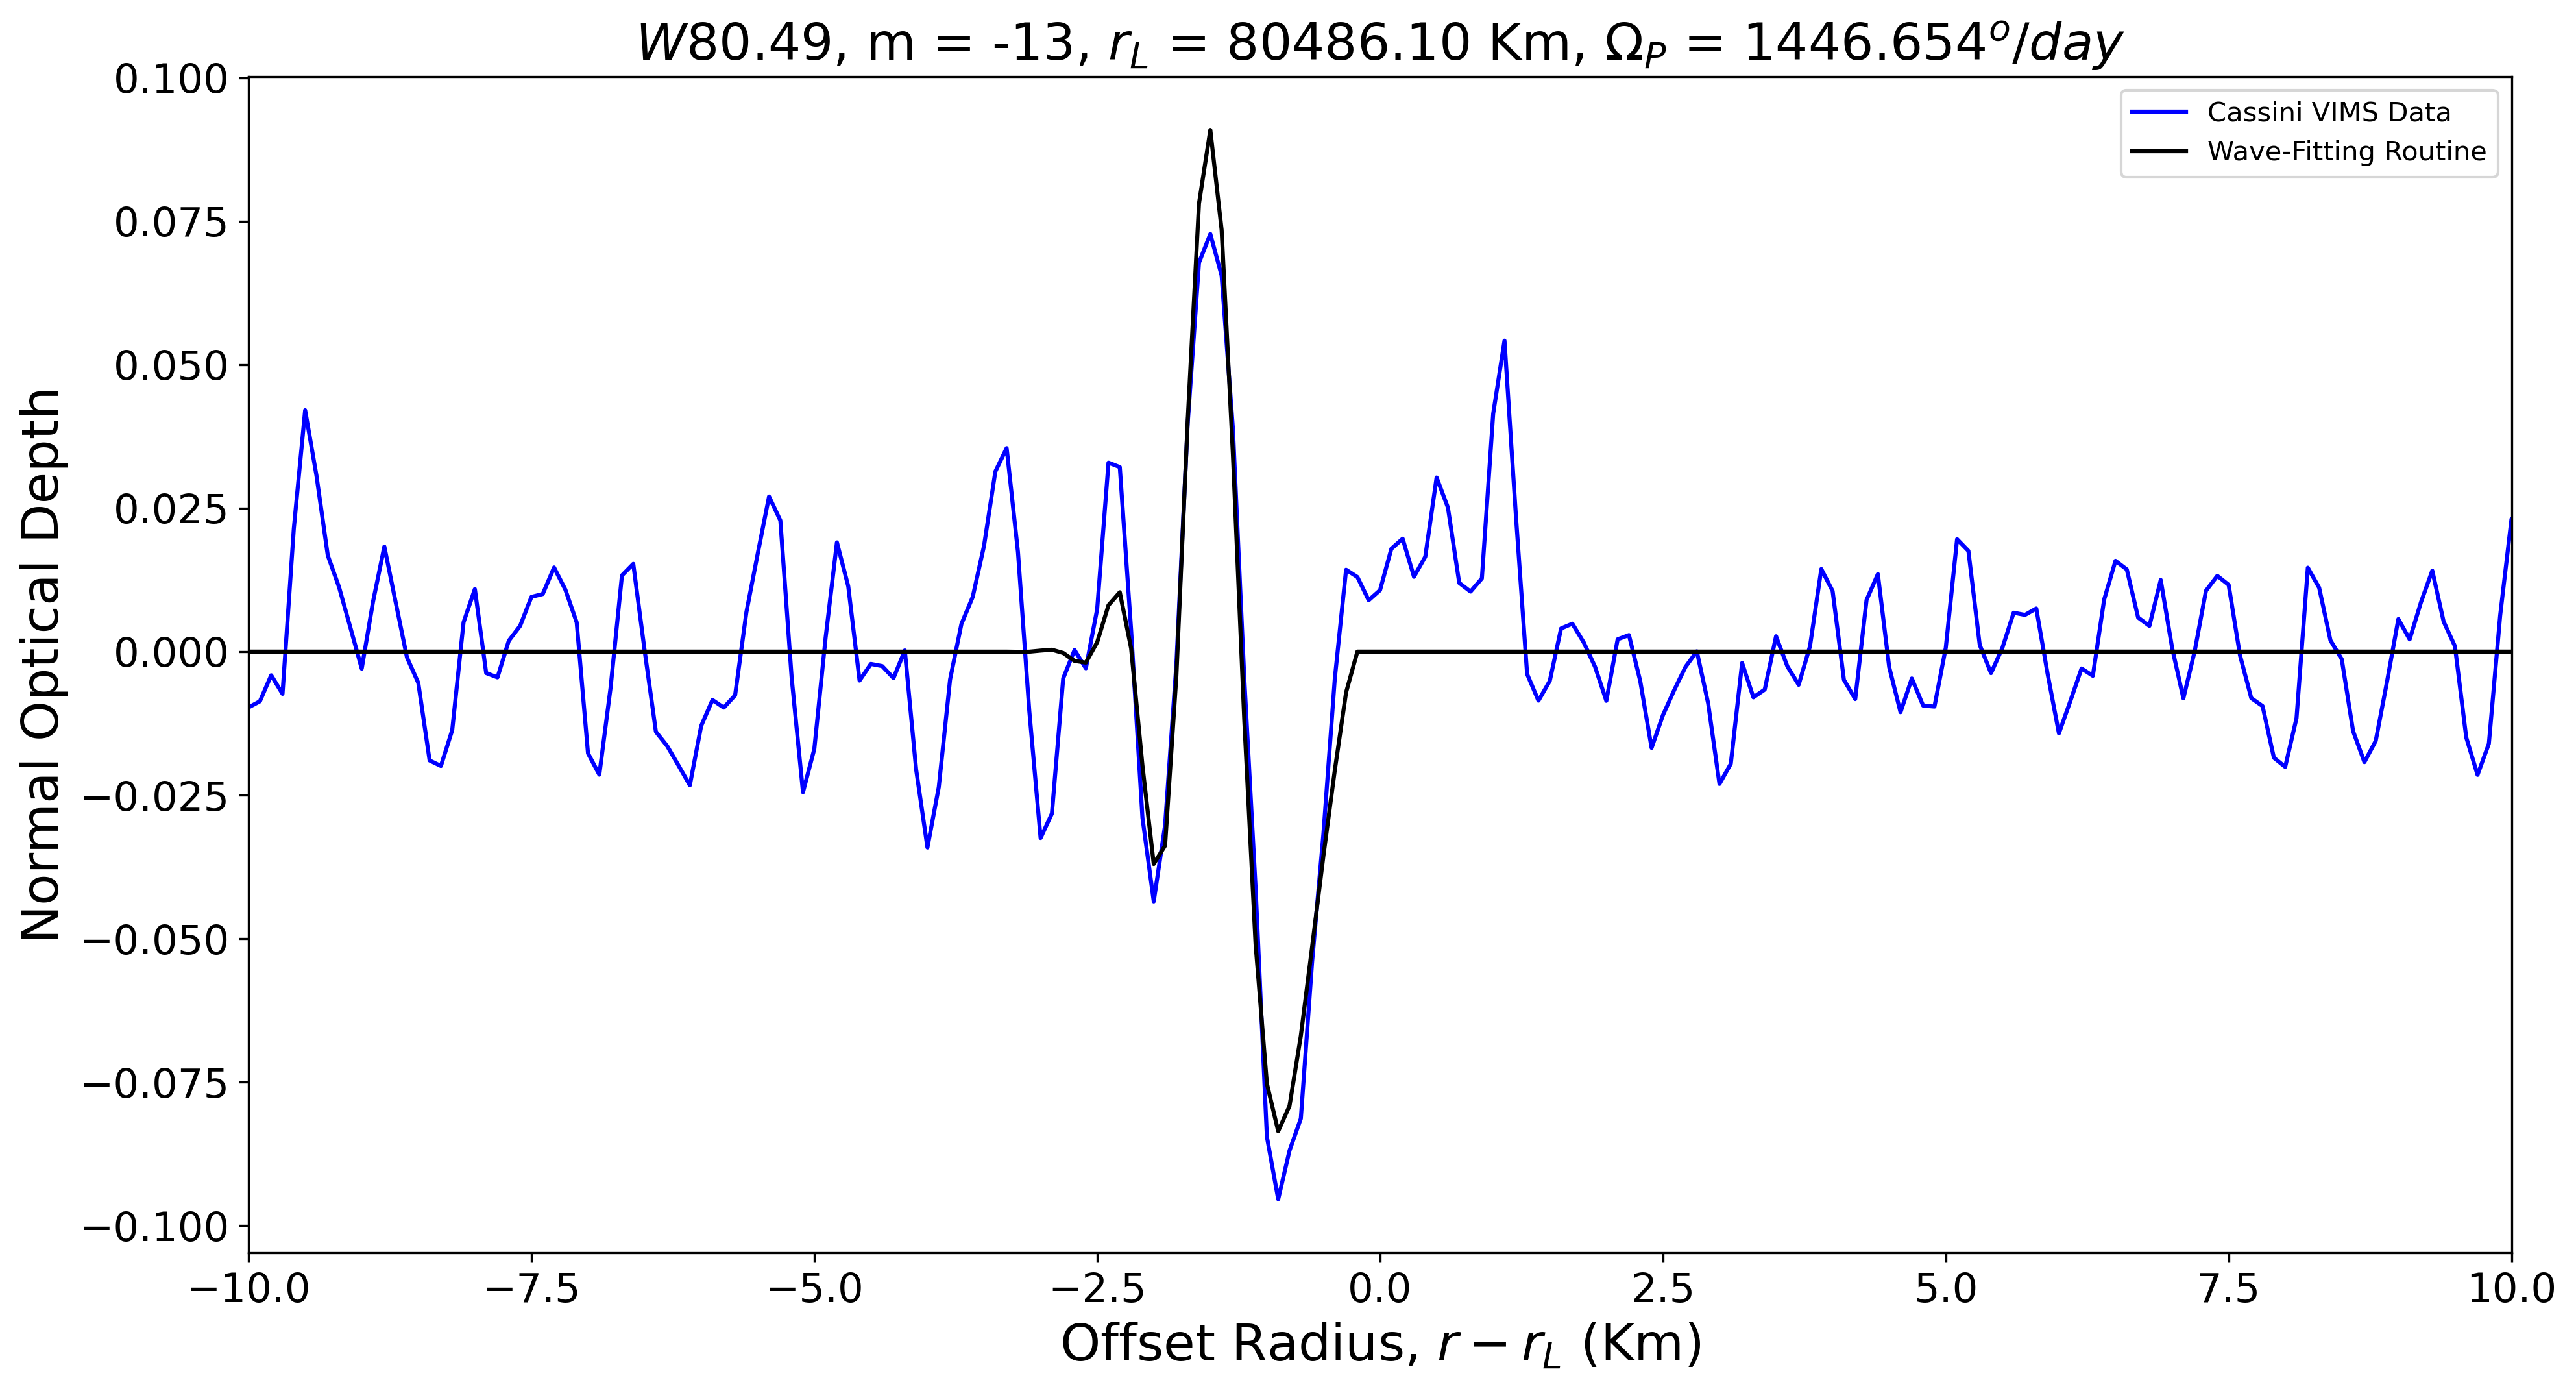
\includegraphics[width=0.3\textwidth, height=0.2\textheight, keepaspectratio]{w8049mp.png}} &
            \subcaptionbox{W80.99}{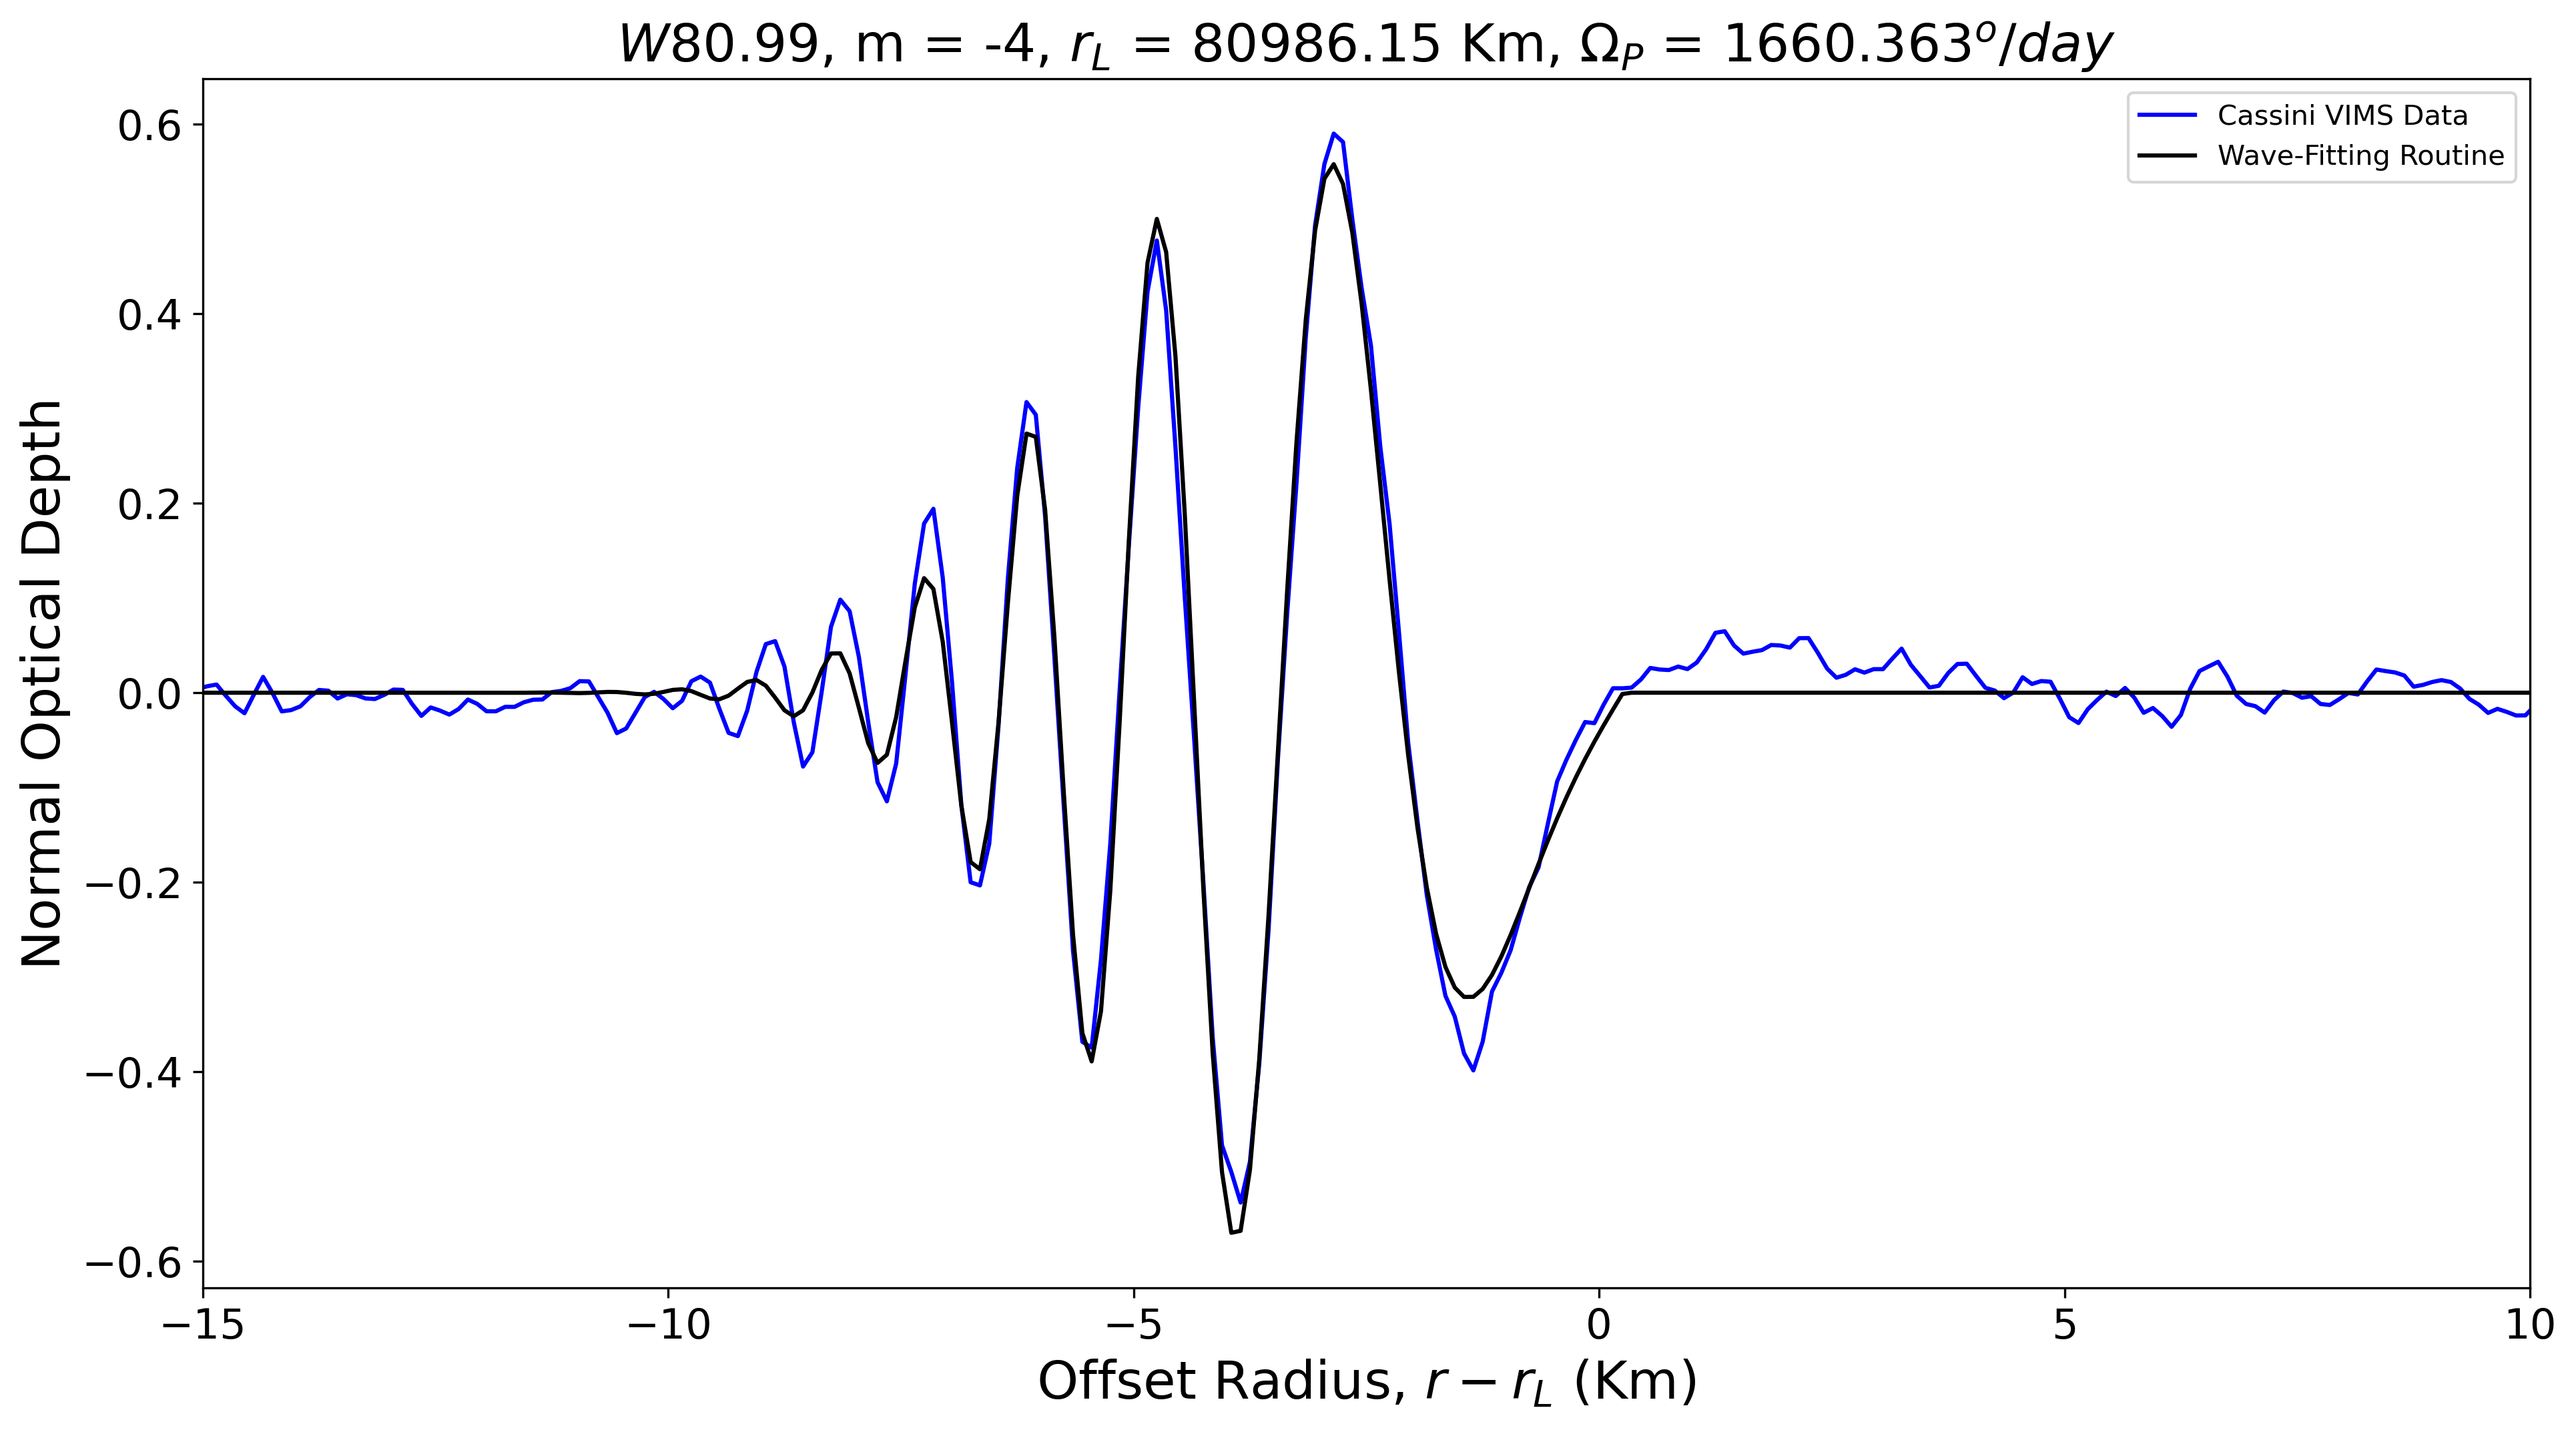
\includegraphics[width=0.3\textwidth, height=0.2\textheight, keepaspectratio]{w8099mp.png}} &
            \subcaptionbox{W81.023A}{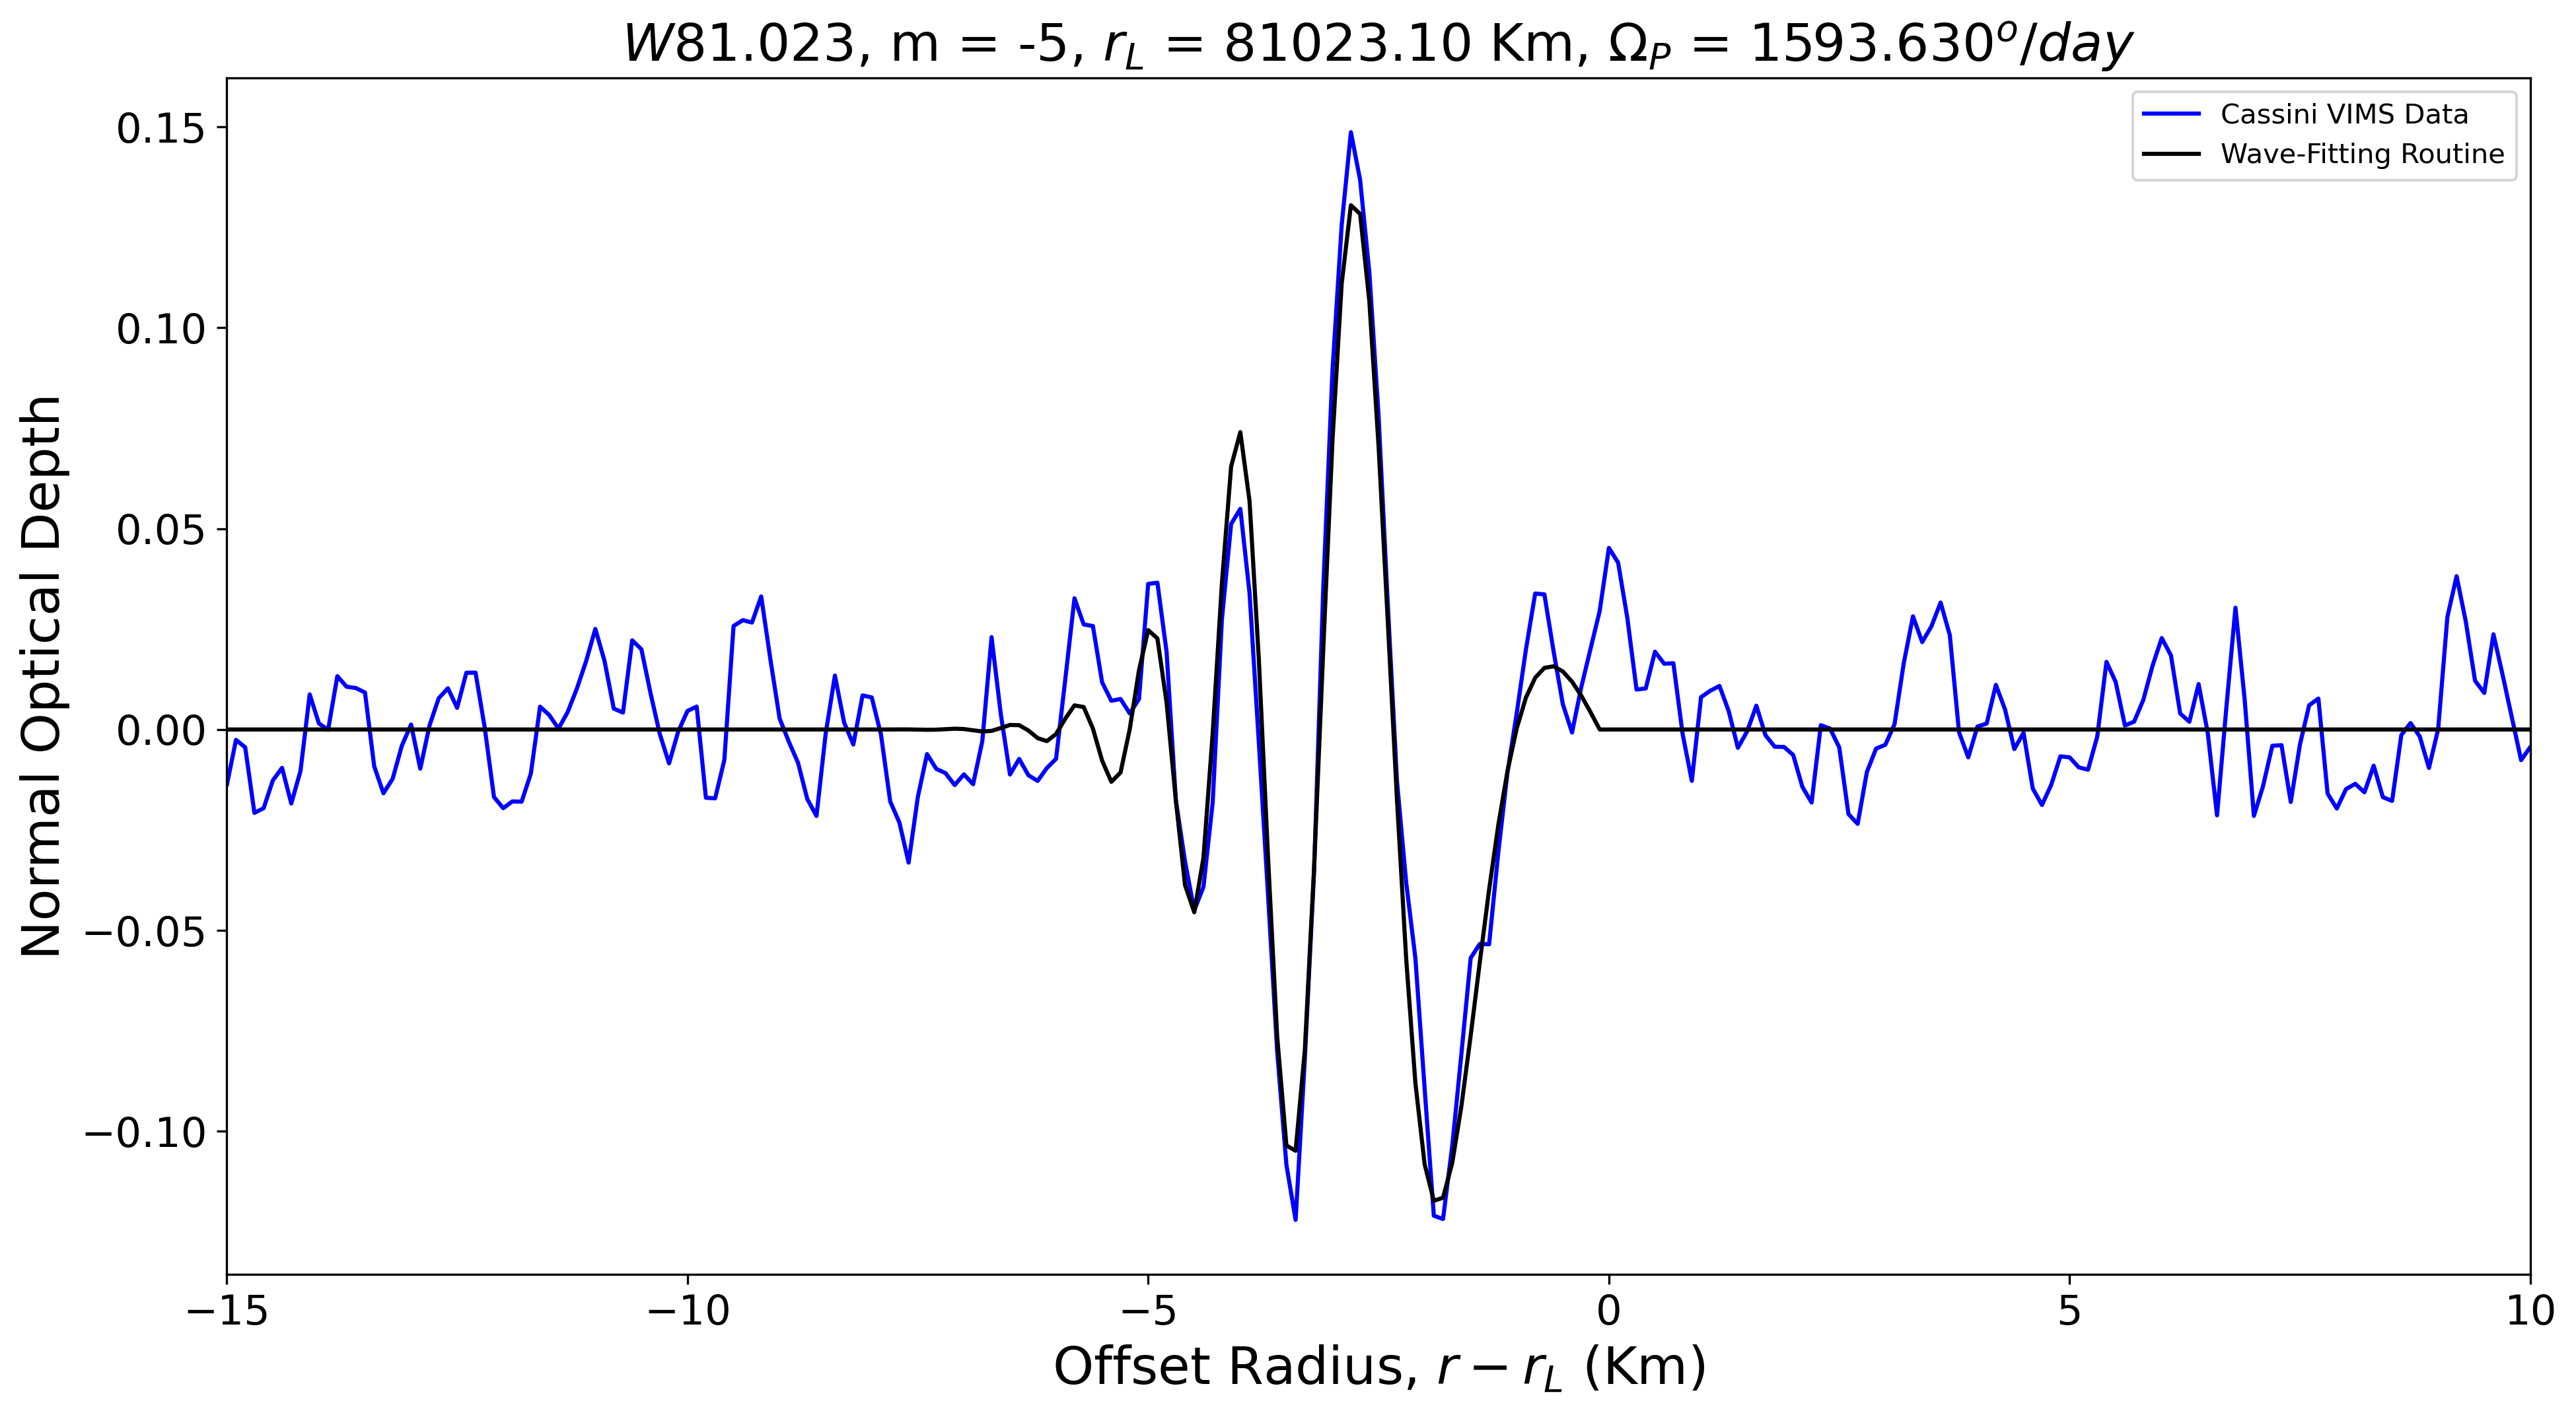
\includegraphics[width=0.3\textwidth, height=0.2\textheight, keepaspectratio]{w81023amp.png}} \\
            \subcaptionbox{W81.024B}{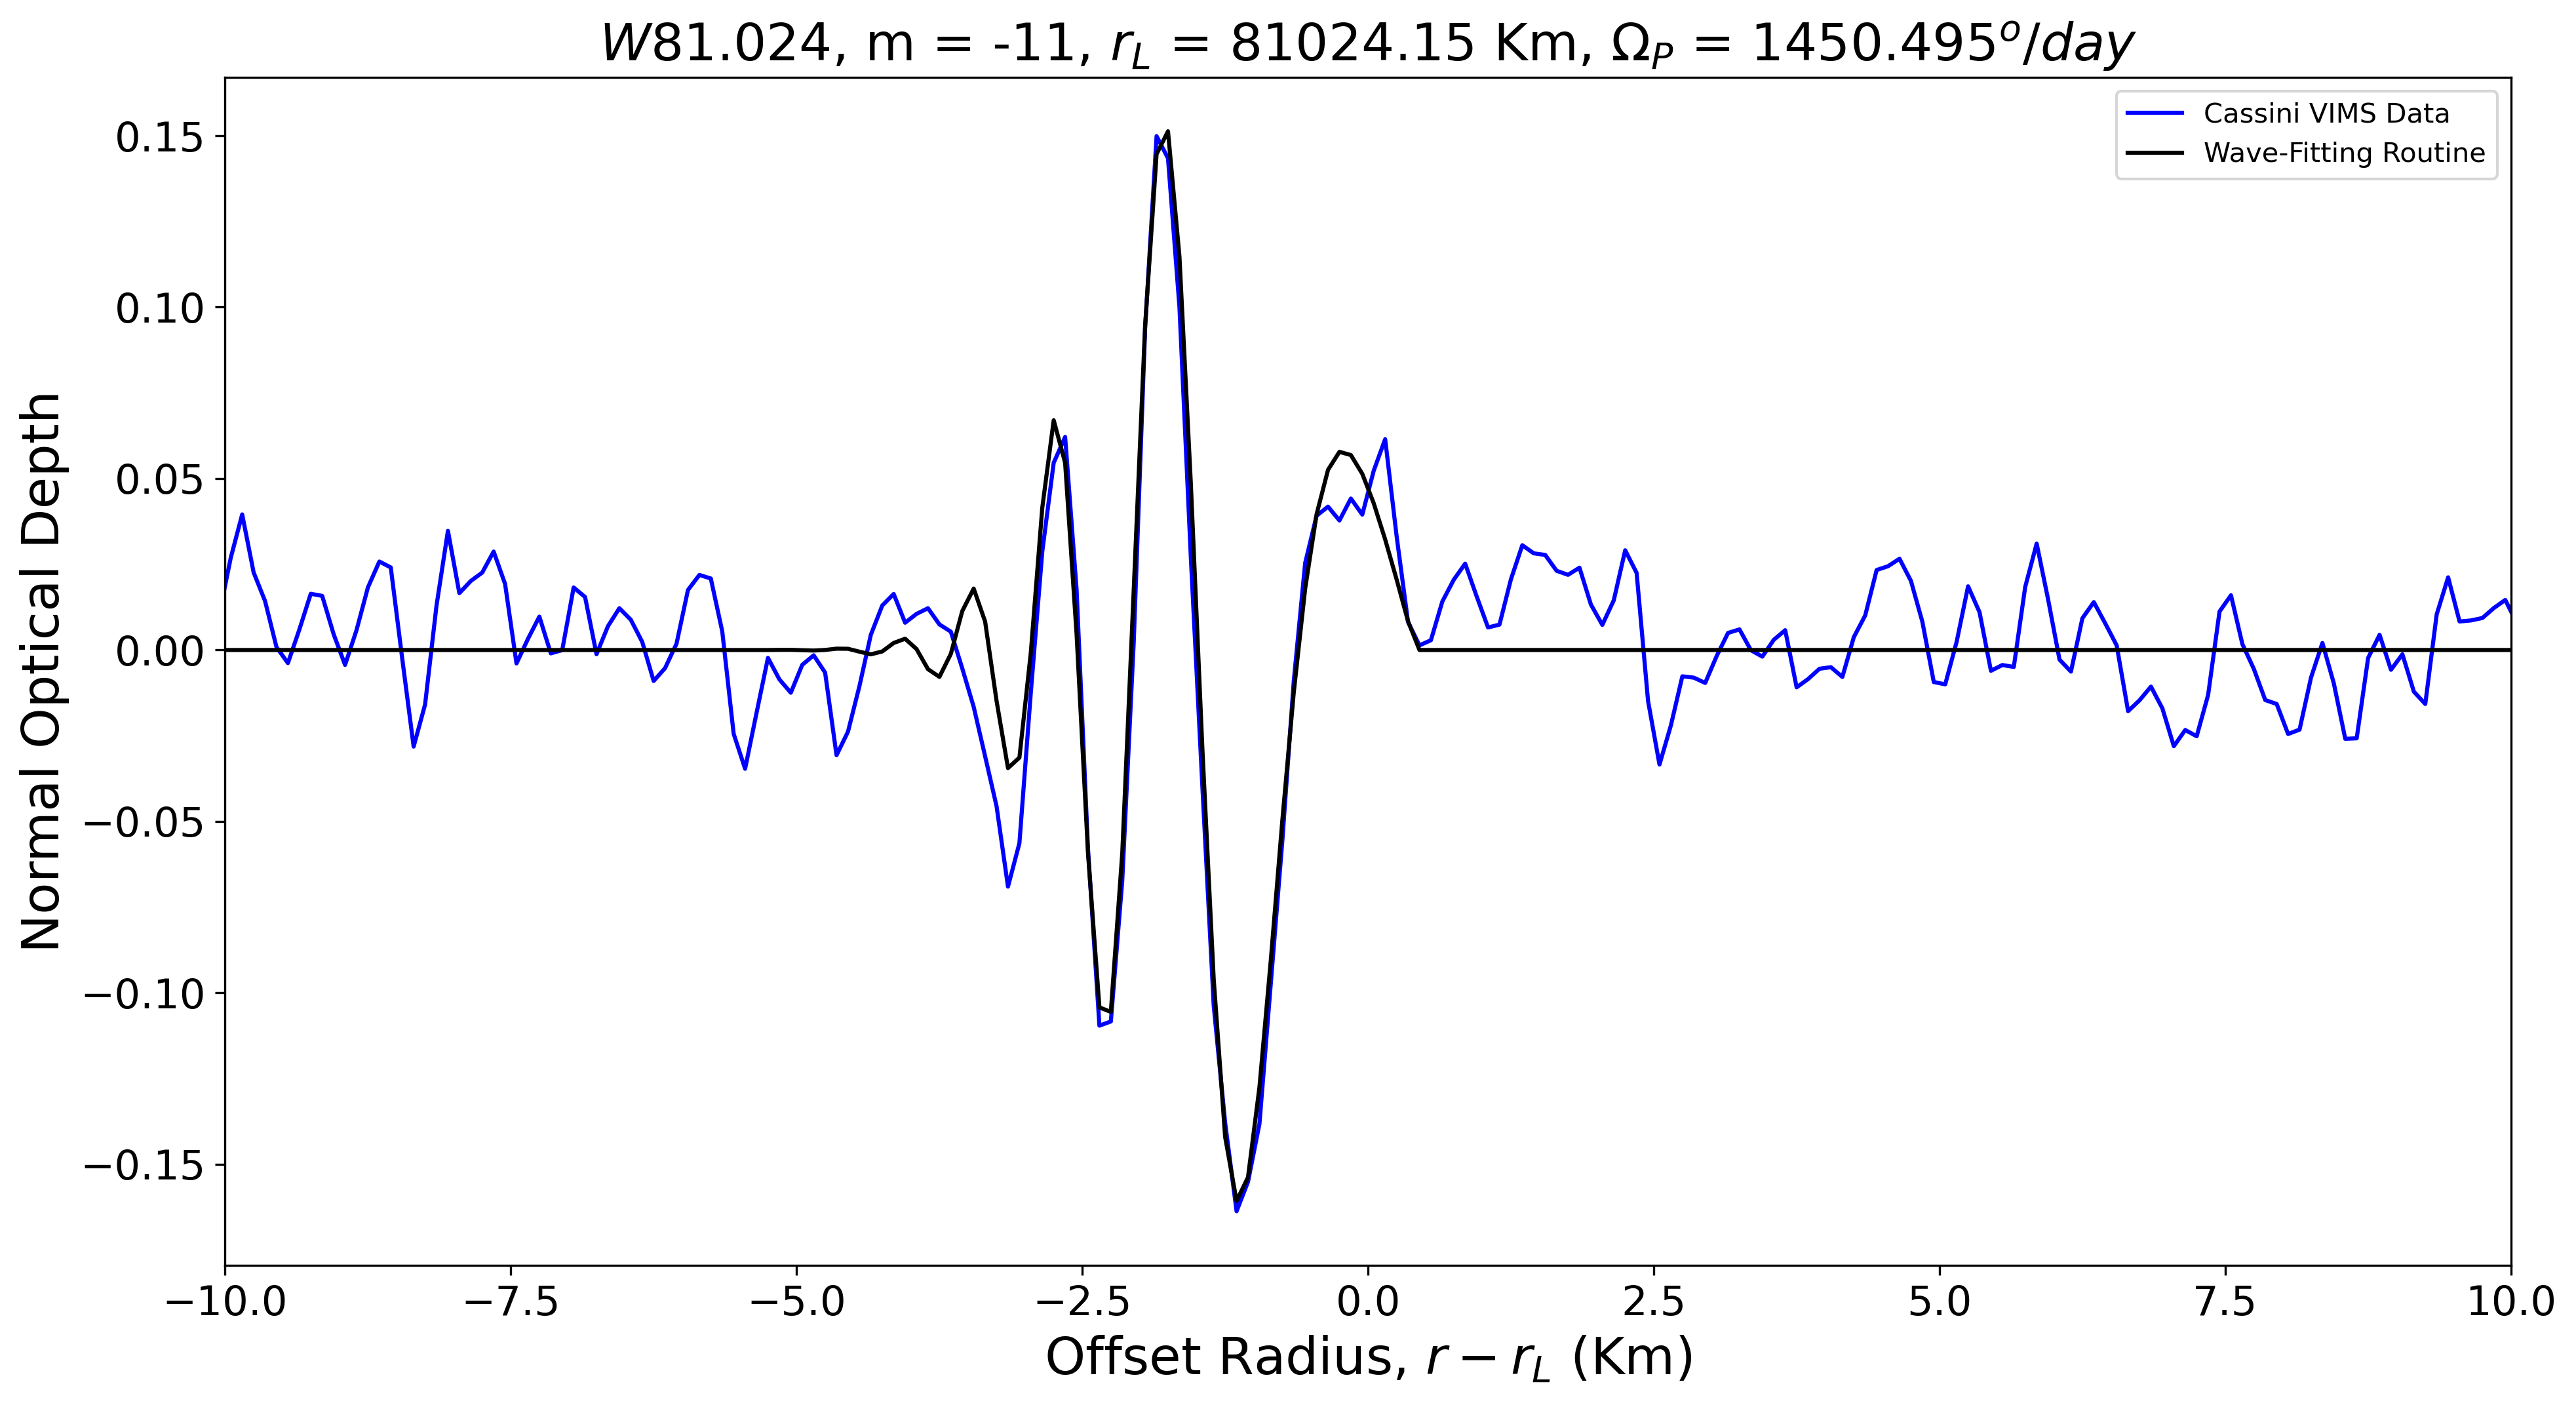
\includegraphics[width=0.3\textwidth, height=0.2\textheight, keepaspectratio]{w81024mp.png}} &
            \subcaptionbox{W81.33}{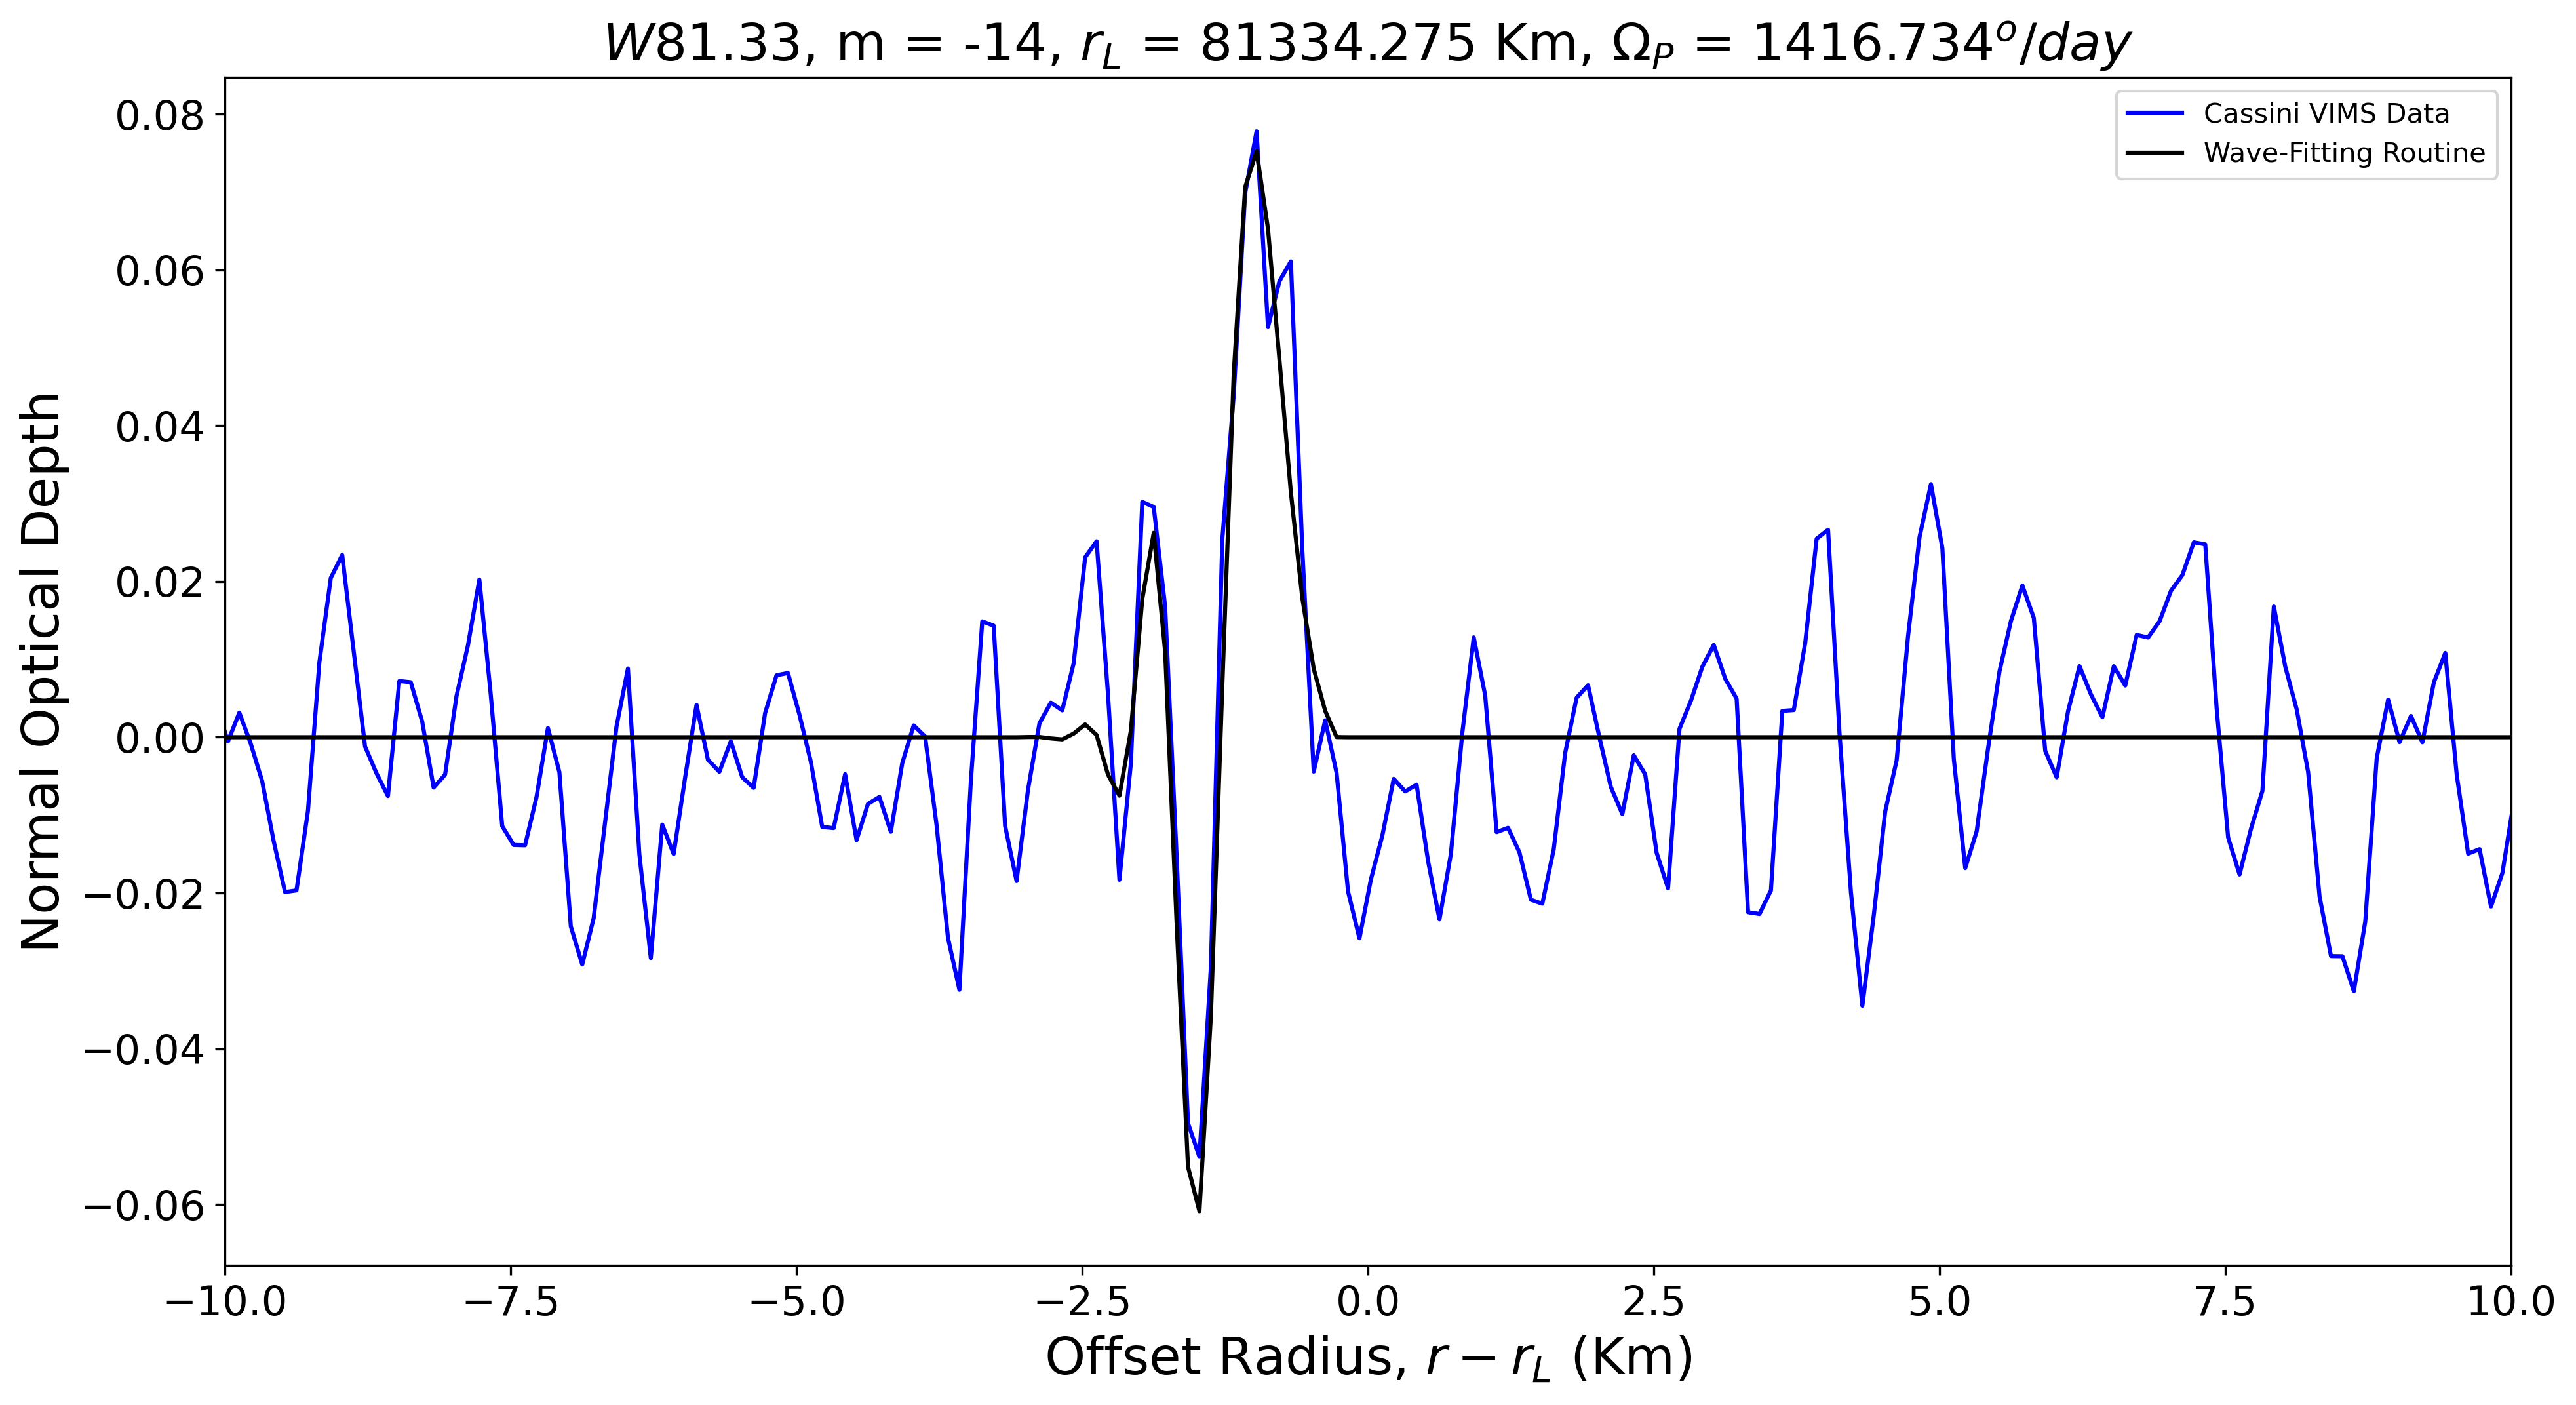
\includegraphics[width=0.3\textwidth, height=0.2\textheight, keepaspectratio]{w8133mp.png}} &
            \subcaptionbox{W81.43}{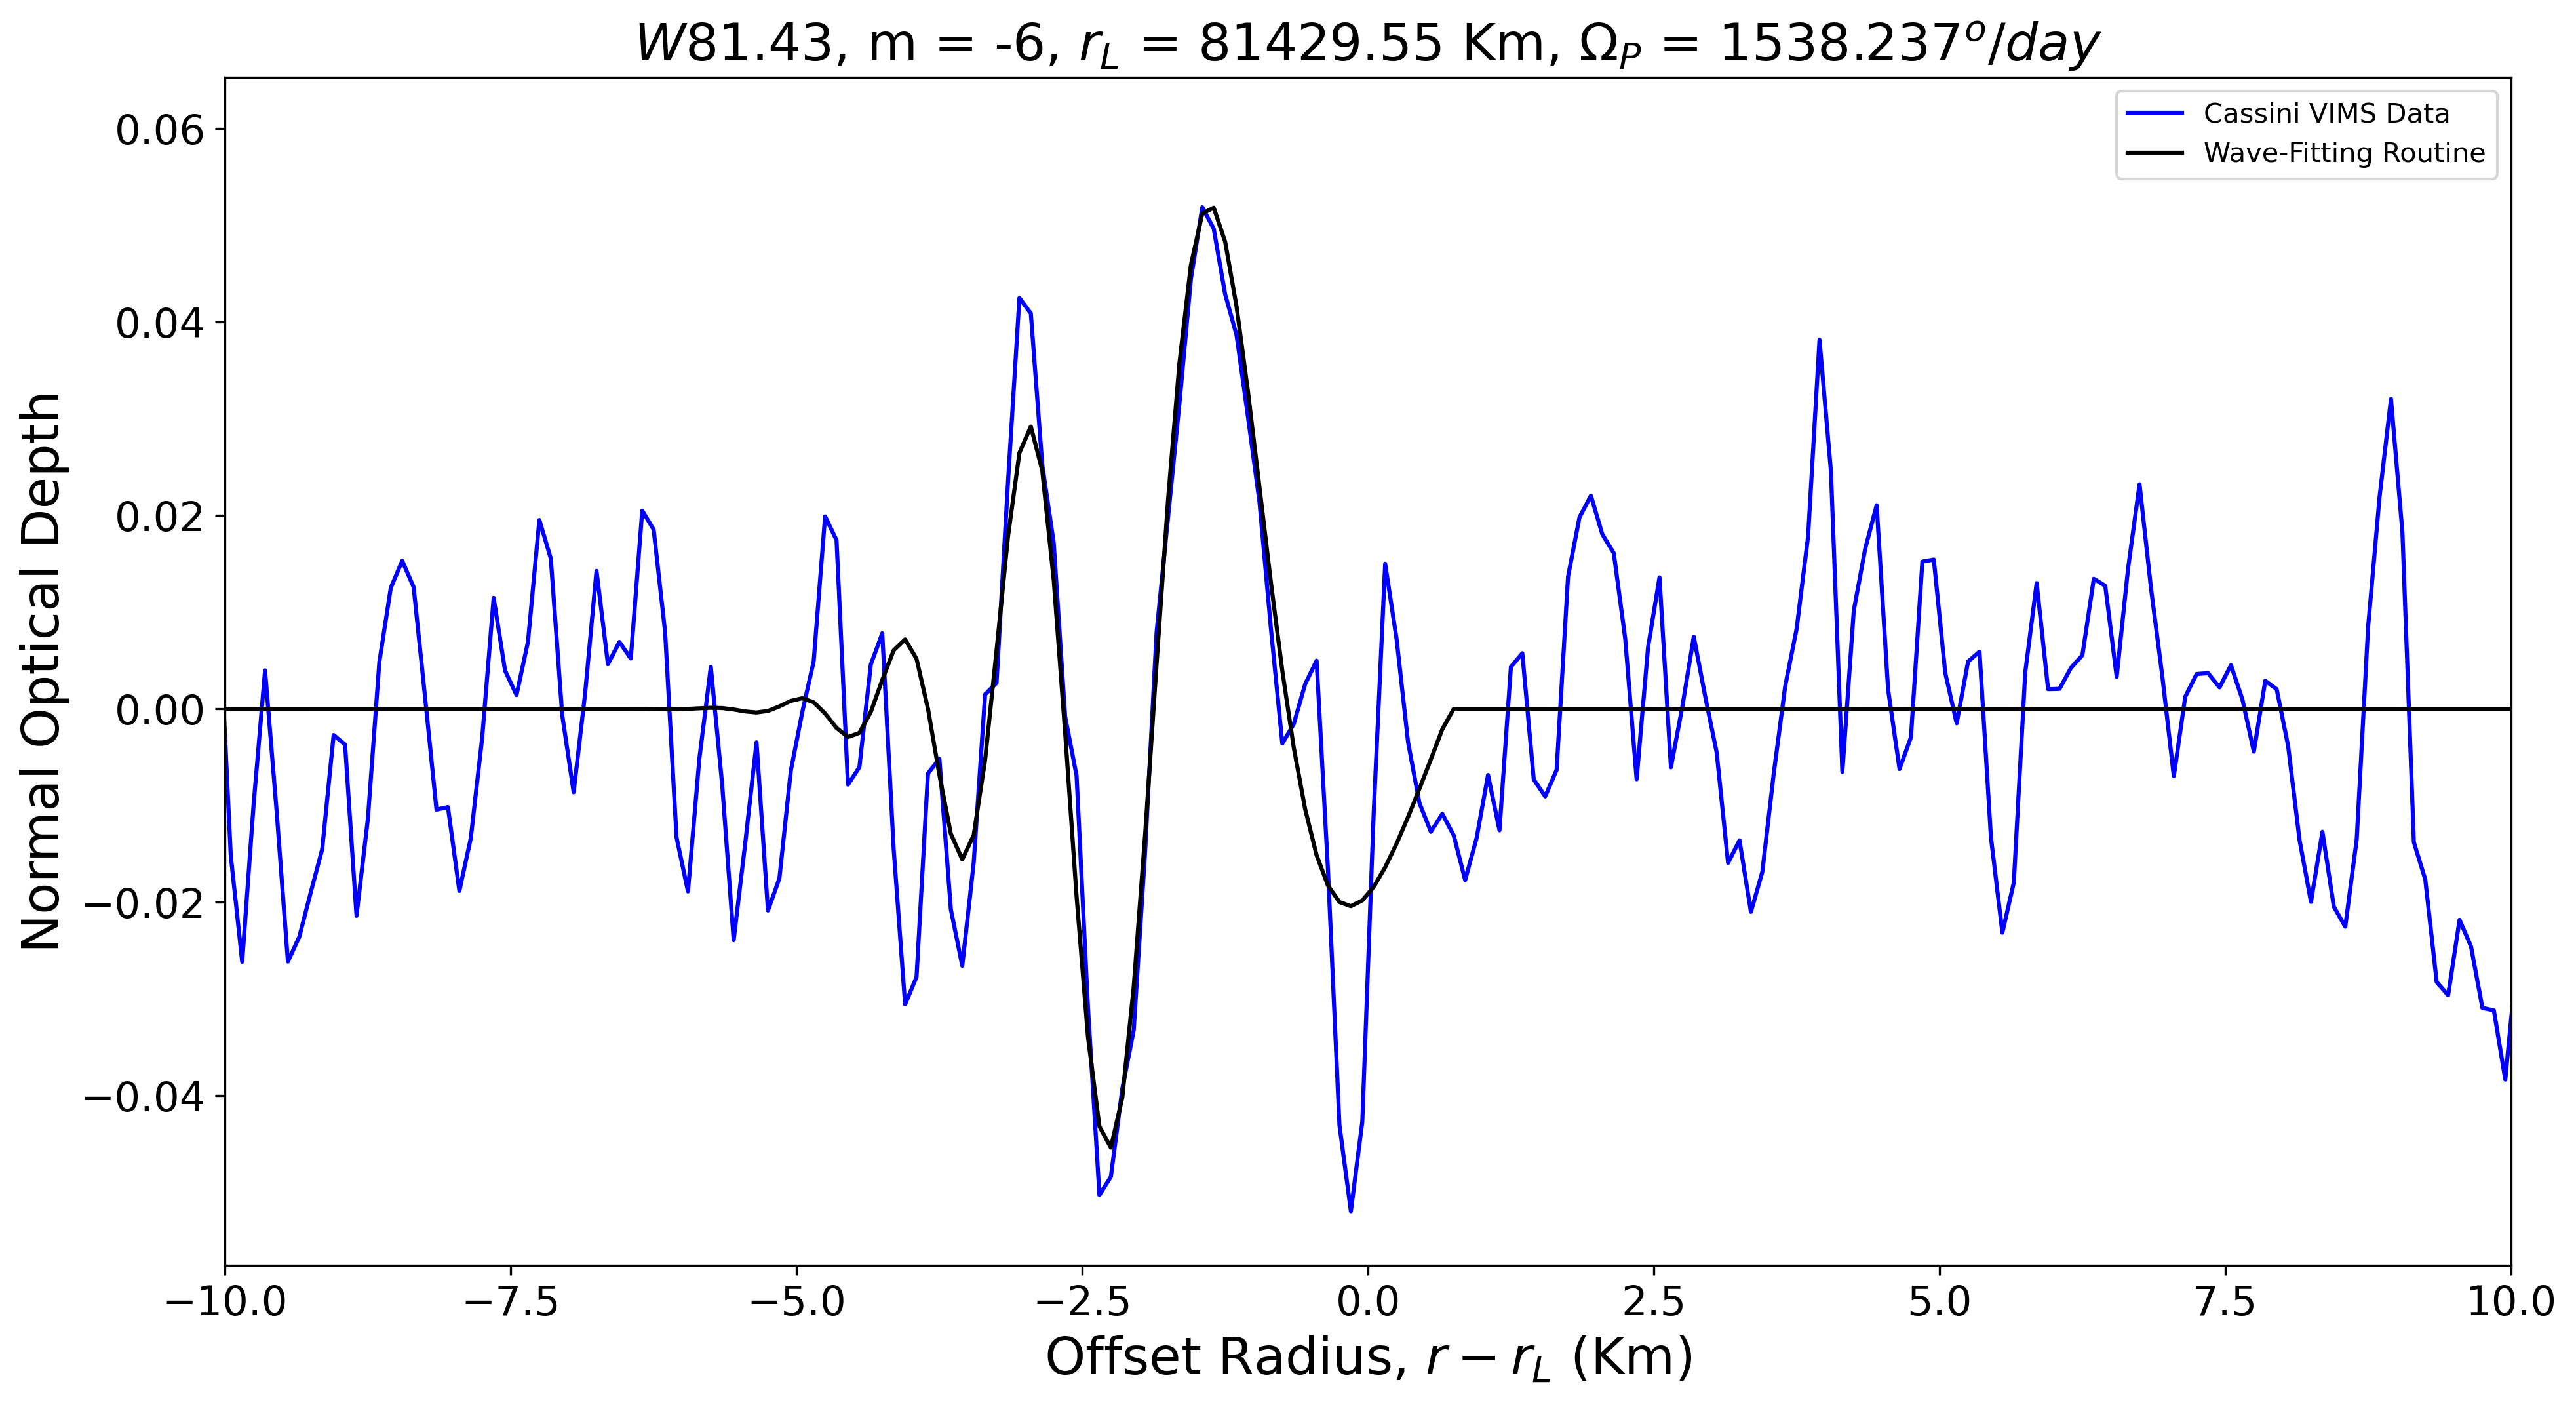
\includegraphics[width=0.3\textwidth, height=0.2\textheight, keepaspectratio]{w8143mp.png}} \\
            \subcaptionbox{W81.96}{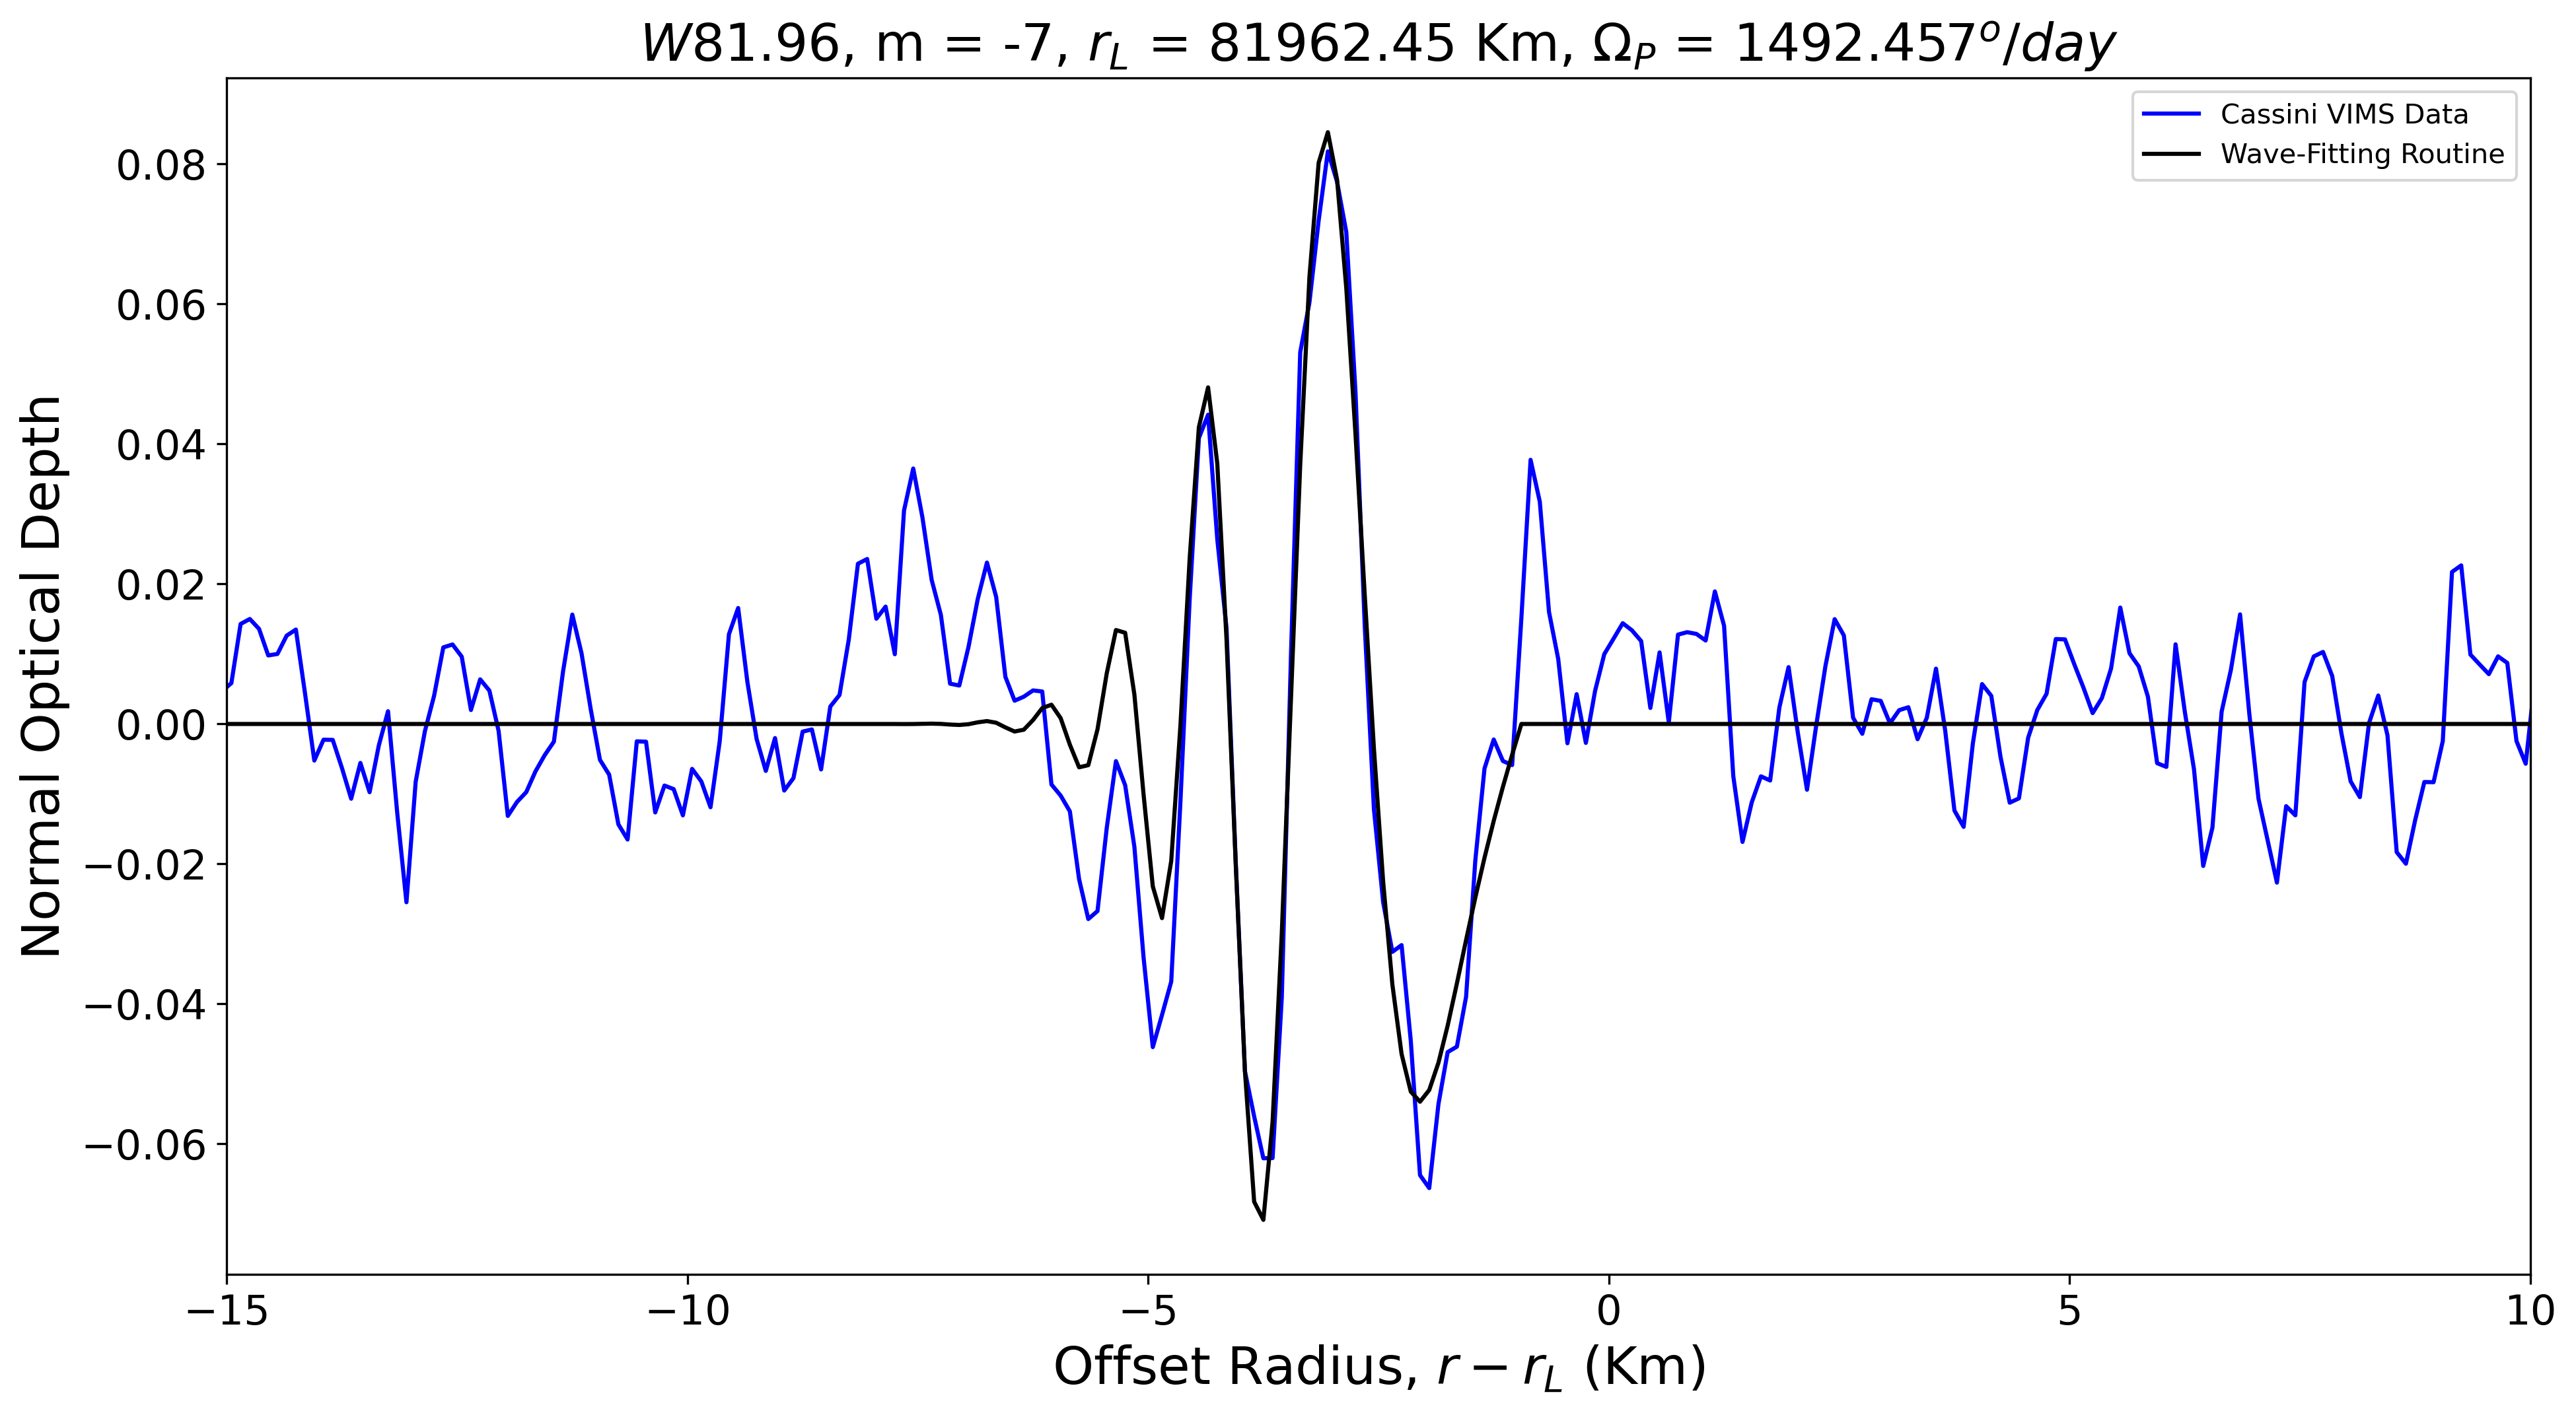
\includegraphics[width=0.3\textwidth, height=0.2\textheight, keepaspectratio]{w8196mp.png}} &
            \subcaptionbox{W82.01}{\includegraphics[width=0.3\textwidth, height=0.2\textheight, keepaspectratio]{w8201mp.png}} &
            \subcaptionbox{W82.06}{\includegraphics[width=0.3\textwidth, height=0.2\textheight, keepaspectratio]{w8206mp.png}} \\
            \subcaptionbox{W82.21}{\includegraphics[width=0.3\textwidth, height=0.2\textheight, keepaspectratio]{w8221mp.png}} &
            \subcaptionbox{W82.53}{\includegraphics[width=0.3\textwidth, height=0.2\textheight, keepaspectratio]{w8253mp.png}} &
            \subcaptionbox{W82.61}{\includegraphics[width=0.3\textwidth, height=0.2\textheight, keepaspectratio]{w8261mp.png}} \\
            \subcaptionbox{W83.09}{\includegraphics[width=0.3\textwidth, height=0.2\textheight, keepaspectratio]{w8309mp.png}} &
            \subcaptionbox{W83.63}{\includegraphics[width=0.3\textwidth, height=0.2\textheight, keepaspectratio]{w8363mp.png}} &
            \subcaptionbox{W84.15}{\includegraphics[width=0.3\textwidth, height=0.2\textheight, keepaspectratio]{w8415mp.png}} \\
            \subcaptionbox{W84.64}{\includegraphics[width=0.3\textwidth, height=0.2\textheight, keepaspectratio]{w8464mp.png}} &
            \subcaptionbox{W87.19}{\includegraphics[width=0.3\textwidth, height=0.2\textheight, keepaspectratio]{w8719mp.png}} &
        \end{tabular}
        \caption{A catalogue of plots from wave-fitting routine exercise for given satellite and planetary resonances. (continued)}
    \end{figure}
}



\paragraph{Bounds for Wave-fitting Routine: Satellite and Planetary Resonances}

\begin{table}
\centering
\vspace{0.01pt} % Adjust the value as needed
\rotatebox{90}{
\normal
%\begin{tabular}{lllll}
\begin{tabular}{|c|c|c|c|c|c|c|c|c|c|}
\hline
\stackon[0pt]{Name}{\stackon[0pt]{Resonance}} & \stackon[0pt]{(Km)}{\stackon[0pt]{Range}{Radial}} & \stackon[0pt]{(Km)}{\stackon[0pt]{Location}{Resonance}} & $l$ & $m$ & $a_{fit,b}$ & $x_{d,b}$ & $\phi_{0,b} (rad)$ & $x_{r,b} (Km)$ & $x_{f,b} (Km)$ \\
\hline
\stackon[0pt]{Resonance}{\stackon[0pt]{Satellite}} & \saturn & \saturn & \saturn & \saturn & \saturn & \saturn & \saturn & \saturn & \saturn \\
\hline
Mimas 4:1 & 74880.00 - 74895.00 &  74890.07 & - & 2 & (0, 1) & (1, 5) & (-2\pi, 2\pi) & (-10, 10) & (0, 4) \\
Pan 2:1 & 85090.00 - 85130.00 & 85105.02 & - & 2 & (0, 1) & (1, 15) & (-2\pi, 2\pi) & (-10, 10) & (0, 4) \\
Atlas 2:1 & 87640.00 - 87650.00 & 87645.68 & - & 2 & (0, 1) & (1, 15) & (-2\pi, 2\pi) & (-10, 10) & (0, 2) \\
Prometheus 4:2 & 88420.00 - 88440.00 & 88434.12 & - & 3 & (0, 1) & (1, 15) & (-2\pi, 2\pi) & (-10, 10) & (0, 3) \\
Mimas 6:2 & 89870.00 - 89890.00 & 89884.00 & - & 3 & (0, 1) & (1, 15) & (-2\pi, 2\pi) & (-10, 10) & (0, 4) \\
Pandora 4:2 & 89887.00 - 89897.00 & 89893.68 & - & 3 & (0, 1) & (1, 15) & (-2\pi, 2\pi) & (-10, 10) & (0, 3) \\
\hline
\stackon[0pt]{Resonance}{\stackon[0pt]{Planetary}} & \saturn & \saturn & \saturn & \saturn & \saturn & \saturn & \saturn & \saturn & \saturn \\
\hline
$W74.51^{av}$ & 74501.00 - 74509.00 & 74506.900 & 12 & -8 & (0, 0.7) & (1, 30) & (-2\pi, 2\pi) &(-10, 10) &(0.5, 2) \\
W74.74 & 74736.00 - 74743.00 & 74739.850 & 15 & 13 & (0, 0.2) & (1, 10) & (-2\pi, 2\pi) & (-10, 10) & (0, 1) \\
W74.75 & 74746.00 - 74748.00 & 74748.300 & 11 & 11 & (0, 0.2) & (1, 35) & (-2\pi, 2\pi) & (-10, 10) & (0, 1) \\
W74.76 & 74752.00 - 74762.00 & 74756.600 & 19 & -11 & (0, 0.2) & (1, 10) & (-2\pi, 2\pi) & (-10, 10) & (0, 1) \\
W75.14 & 75142.00 - 75144.00 & 75143.000 & 16 & -10 & (0, 0.8) & (1, 40) & (-2\pi, 2\pi) & (-10, 10) & (0, 1) \\
W76.02A & 76016.00 - 76018.00 & 76018.100 & 13 & -9 & (0, 0.6) & (1, 10) & (-2\pi, 2\pi) & (-10, 10) & (0, 2) \\
W76.44 & 76433.00 - 76436.00 & 76435.400 & 2 & -2 & (0, 0.6) & (1, 25) & (-2\pi, 2\pi) & (-10, 10) & (0, 2) \\
$W76.46^{av}$ & 76457.00 - 76462.00 & 76459.500 & 9 & -7 & (0, 0.4) & (1, 40) & (-2\pi, 2\pi) & (-10, 10) & (0, 1) \\
W77.34 & 77337.00 - 77339.00 & 77338.900 & 14 & -10 & (0, 0.3) & (1, 35) & (-2\pi, 2\pi) & (-10, 10) & (0, 1) \\
W78.51 & 78503.00 - 78509.00 & 78506.750 & 15 & -11 & (0, 0.8) & (1, 20) & (-2\pi, 2\pi) & (-10, 10) & (0, 1) \\
W79.04 & 79039.00 - 79045.00 & 79042.300 & 11 & -9 & (0, 0.4) & (1, 25) & (-2\pi, 2\pi) & (-10, 10) & (0, 1) \\
W79.55 & 79546.00 - 79550.00 & 79548.920 & 16 & -12 & (0, 0.2) & (1, 25) & (-2\pi, 2\pi) & (-10, 10) & (0, 1) \\
W80.49 & 80484.00 - 80488.00 & 80486.100 & 17 & -13 & (0, 0.3) & (1, 25) & (-2\pi, 2\pi) & (-10, 10) & (0, 1) \\
W80.99 & 80983.00 - 80989.00 & 80986.150 & 4 & -4 & (0, 0.2) & (1, 25) & (-2\pi, 2\pi) & (-10, 10) & (0, 2) \\
W81.023A & 81018.00 - 81030.00 & 81023.100 & 5 & -5 & (0, 0.2) & (1, 25) & (-2\pi, 2\pi) & (-10, 10) & (0, 2) \\
W81.024B & 81018.00 - 81030.00 & 81024.150 & 13 & -11 & (0, 0.3) & (1, 25) & (-2\pi, 2\pi) & (-10, 10) & (0, 1) \\
W81.33 & 81333.00 - 81336.00 & 81334.275 & 18 & -14 & (0, 0.3) & (1, 25) & (-2\pi, 2\pi) & (-10, 10) & (0, 1) \\
W81.43 & 81420.00 - 81430.00 & 81429.550 & 6 & -6 & (0, 0.2) & (1, 30) & (-2\pi, 2\pi) & (-10, 10) & (0, 2) \\
W81.96 & 81959.00 - 81965.00 & 81962.450 & 7 & -7 & (0, 0.1) & (1, 15) & (-2\pi, 2\pi) & (-5, 0) & (0, 2) \\
W82.01 & 82004.00 - 82009.00 & 82007.750 & 3 & -3 & (0, 0.2) & (1, 5) & (-2\pi, 2\pi) & (-10, 10) & (0, 4) \\
W82.06 & 82055.00 - 82065.00 & 82059.400 & 3 & -3 & (0, 0.5) & (1, 40) & (-2\pi, 2\pi) & (-10, 10) & (0, 3) \\
W82.21 & 82187.50 - 82207.51 & 82207.500 & 3 & -3 & (0, 0.3) & (1, 6) & (-2\pi, 2\pi) & (-15, 15) & (0, 4) \\
W82.53 & 82510.00 - 82530.00 & 82528.750 & 8 & -8 & (0, 0.1) & (1, 15) & (-2\pi, 2\pi) & (-10, 10) & (0, 2) \\
W82.61 & 82606.00 - 82608.00 & 82607.750 & 15 & -13 & (0, 0.2) & (1, 25) & (-2\pi, 2\pi) & (-10, 10) & (0, 2) \\
W83.09 & 83086.00 - 83096.00 & 83090.650 & 9 & -9 & (0, 0.2) & (1, 25) & (-2\pi, 2\pi) & (-10, 10) & (0, 2) \\
W83.63 & 83612.02 - 83637.02 & 83632.020 & 10 & -10 & (0, 0.3) & (1, 20) & (-2\pi, 2\pi) & (-10, 10) & (0, 2) \\
W84.15 & 84140.00 - 84150.00 & 84147.100 & 11 & -11 & (0, 0.2) & (1, 25) & (-2\pi, 2\pi) & (-10, 10) & (0, 1) \\
W84.64 & 84630.00 - 84650.00 & 84643.200 & 2 & -2 & (0, 0.3) & (1, 25) & (-2\pi, 2\pi) & (-10, 10) & (0, 3) \\
W87.19 & 87170.00 - 87210.00 & 87192.800 & 2 & -2 & (0, 0.2) & (1, 40) & (-2\pi, 2\pi) & (-10, 10) & (0, 3) \\
\hline
\end{tabular}
}
\caption{Wave-fit bounds for satellite and planetary resonances.}
\end{table}


\subsection{Additional Data}
\label{subsec:data}

% Insert your additional data here
%\subsection{Code Snippets}
%\label{subsec:code}
% Insert your code snippets here

\subsection{Mathematics of log-linear scatter plots with error bars}
A log-linear plot, also known as a semi-logarithmic plot, is a visualization technique commonly used in various scientific fields to represent data that covers a wide range of values. It combines a logarithmic scale along one axis (usually the y-axis) with a linear scale along the other axis (usually the x-axis). 

The principle behind the log-linear plot lies in the fact that using a logarithmic scale for one of the axes allows for a better representation of data that spans several orders of magnitude. In such plots, the relationship between the plotted variable and the axis is not linear but logarithmic. This means that equal distances on the axis correspond to equal ratios of the plotted variable, rather than equal differences.

\textbf{Logarithmic Scaling}:
In a log-linear plot, one axis (typically the y-axis) is scaled logarithmically. This means that instead of representing values directly, the logarithms of those values are plotted along the logarithmic axis. For example, if $y = \lambda a^{\gamma x}$, taking the logarithm (base $b$) of both sides yields:
     \[ \log_b(y) = \log_b(\lambda) + \gamma x \]
Here, $\log_b$ denotes the logarithm base $b$, which could be $\ln$ (natural logarithm), $\log_{10}$ (common logarithm), or any other base. This equation represents a linear relationship between $\log_b(y)$ and $x$, with slope $\gamma$ and intercept $\log_b(\lambda)$.

\textbf{Linear Regression on Log-Transformed Data}:
Given data points $(x_i, y_i)$, where $y_i$ follows a logarithmic relationship with $x_i$, we transform the data by taking the logarithm of the dependent variable:
     \[ \log_b(y_i) = \log_b(\lambda) + \gamma x_i + \epsilon_i \]
Here, $\epsilon_i$ represents the error associated with each data point. We can then perform linear regression on the transformed data to find the best-fit line, typically using the least squares method.

\textbf{Error Analysis}:
The derivation of the equation for the error bars on $\log_b(y_i)$ involves considering how small changes in $y_i$ affect the logarithm of $y_i$ \cite{stewart2010calculus}\cite{taylor2022introduction}\cite{press2007numerical}. We can use calculus to find the relative change in $\log_b(y_i)$ when $y_i$ changes by $\sigma_i$.

Let's denote $\Delta \log_b(y_i)$ as the change in $\log_b(y_i)$ due to a change of $\sigma_i$ in $y_i$. Then:

\[
\Delta \log_b(y_i) = \frac{d}{dy_i} \log_b(y_i) \cdot \sigma_i
\]

Differentiating $\log_b(y_i)$ with respect to $y_i$, we get:

\[
\frac{d}{dy_i} \log_b(y_i) = \frac{1}{y_i \ln(b)}
\]

Now, multiplying both sides by $\sigma_i$:

\[
\Delta \log_b(y_i) = \frac{\sigma_i}{y_i \ln(b)}
\]

This represents the change in $\log_b(y_i)$ due to the error $\sigma_i$ in $y_i$. For symmetric error bars, we take the error bars to be $\pm \Delta \log_b(y_i)$, so the error bars on $\log_b(y_i)$ are $\pm \frac{\sigma_i}{{y_i \ln(b)}}$\cite{bevington2003data,press2007numerical,taylor2022introduction}. The concept of the semi-log plot and its error analysis can be seen in figures (16) and (17).
%...........................................................................



%...........................................................................
\bibliographystyle{plain}
\bibliography{reference}

\end{document}


%This study explores the possibility that Saturn's rings function as seismographs, recording gravitational signals resulting from the acoustic oscillation modes of the planet. Certain spiral density waves in Saturn's rings are generated through resonances with planetary normal modes, making them valuable probes of Saturn's internal structure. Previous research has primarily focused on the rotation rates of these waves, which yield precise measurements of Saturn's oscillation frequencies. However, other characteristics of these waves also contain valuable information about the planet's interior. In this work, we have investigated the amplitudes of the ring waves by analyzing high signal-to-noise profiles obtained from Cassini's Visual and Infrared Mapping Spectrometer (VIMS) occultations. By fitting these profiles, we have successfully determined the amplitudes of the perturbing potentials responsible for generating numerous waves. Furthermore, we have estimated the corresponding non-zonal gravitational spherical harmonic coefficients that generate approximately a dozen of these spiral density waves. The observed spectrum primarily consists of the fundamental mode (f-mode) oscillations with relatively low spherical harmonic degrees. Analyzing these oscillations provides insights into the excitation mechanisms of such oscillations within Saturn's interior. By combining these findings with the precise measurements of oscillation frequencies from the rotation rates, we can gain a comprehensive understanding of Saturn's internal structure and dynamics.

%Keywords: Saturn, rings, seismographs, acoustic oscillation modes, spiral density waves, planetary normal modes, oscillation frequencies, spherical harmonic coefficients, Cassini, VIMS, occultations, internal structure, f-mode oscillations.